\documentclass[11pt, a4paper, twoside, openany]{book}

% ═══════════════════════════════════════════════════════════
%  Seven Sketches in Compositionality — 한국어 번역 디자인 시스템
%  Design Sample: Chapter 1.1 (Generative Effects)
% ═══════════════════════════════════════════════════════════

% ─── 여백 ───
\usepackage[
  top=27mm,
  bottom=22mm,
  inner=28mm,
  outer=24mm,
  bindingoffset=4mm,
  headheight=14pt,
  headsep=12pt
]{geometry}

% ─── 한글 ───
\usepackage{kotex}
\usepackage{fontspec}

% ─── 폰트 ───
\setmainfont{Noto Serif CJK KR}[
  UprightFont={Noto Serif CJK KR},
  BoldFont={Noto Serif CJK KR Bold},
  Ligatures=TeX,
]
\setsansfont{Noto Sans CJK KR}[
  UprightFont={Noto Sans CJK KR},
  BoldFont={Noto Sans CJK KR Bold},
  Ligatures=TeX,
]
\setmonofont{Noto Sans Mono CJK KR}[Scale=0.85]

% ─── 수식 ───
\usepackage{amsmath, amssymb, amsthm}

% ─── 그래픽 ───
\usepackage{graphicx}
\graphicspath{{images/}}
\usepackage{tikz}
\usetikzlibrary{arrows.meta, positioning, shapes, calc, decorations.pathreplacing, backgrounds}

% ─── 색상 팔레트 (원서 톤 반영: 앰버+블루) ───
\usepackage{xcolor}
\definecolor{ctamber}{HTML}{B8860B}      % 원서 참조 링크 색
\definecolor{ctblue}{HTML}{2C5F8A}       % 챕터/섹션 강조
\definecolor{ctdark}{HTML}{1A1A2E}       % 본문 제목
\definecolor{ctlight}{HTML}{F8F4EC}      % 정의 박스 배경
\definecolor{ctexer}{HTML}{E8F5E9}       % 연습문제 배경
\definecolor{ctexample}{HTML}{FFF8E1}    % 예제 배경
\definecolor{ctnote}{HTML}{F3E5F5}       % 역주 배경
\definecolor{ctgray}{HTML}{607D8B}       % 헤더/캡션
\definecolor{ctdeep}{HTML}{1B3A5C}       % 딥리서치
\definecolor{ctred}{HTML}{C62828}        % 경고/강조

% ─── 한글 줄바꿈 최적화 ───
\XeTeXlinebreaklocale "ko"
\XeTeXlinebreakskip 0pt plus 3pt
\emergencystretch 5em
\tolerance=2000
\hyphenpenalty=50
\exhyphenpenalty=50
\doublehyphendemerits=10000
\finalhyphendemerits=5000
\setlength{\hfuzz}{2pt}

% ─── 행간 ───
\linespread{1.55}
\setlength{\parindent}{1em}
\setlength{\parskip}{2pt plus 1pt}

% ─── 박스 디자인 (tcolorbox) ───
\usepackage[most]{tcolorbox}

% ◆ 정의 (Definition) — 차분한 크림색 배경
\newtcolorbox{definitionbox}[1][]{
  enhanced, colback=ctlight, colframe=ctamber!70!black,
  coltitle=white, fonttitle=\sffamily\bfseries\small,
  title={#1},
  attach boxed title to top left={yshift=-2mm, xshift=4mm},
  boxed title style={colback=ctamber!80, sharp corners, boxrule=0pt},
  sharp corners, boxrule=0.6pt, breakable,
  left=10pt, right=10pt, top=10pt, bottom=8pt,
}

% ◆ 연습문제 (Exercise) — 녹색 계열
\newtcolorbox{exercisebox}[1][]{
  enhanced, colback=ctexer, colframe=ctblue!40!green!60,
  fonttitle=\sffamily\bfseries\small,
  title={#1},
  sharp corners, boxrule=0pt, leftrule=4pt, breakable,
  left=10pt, right=10pt, top=8pt, bottom=8pt,
}

% ◆ 예제 (Example) — 따뜻한 노란색
\newtcolorbox{examplebox}[1][]{
  enhanced, colback=ctexample, colframe=ctamber!50,
  fonttitle=\sffamily\bfseries\small,
  title={#1},
  sharp corners, boxrule=0pt, leftrule=4pt, breakable,
  left=10pt, right=10pt, top=8pt, bottom=8pt,
}

% ◆ 역주 (Translator's Note)
\newtcolorbox{translatornote}[1][]{
  enhanced, colback=ctnote!50, colframe=ctgray!40,
  fonttitle=\sffamily\bfseries\small,
  title={\raisebox{-0.5pt}{\textsf{*}} 역주},
  sharp corners, boxrule=0pt, leftrule=3pt, breakable,
  left=10pt, right=10pt, top=6pt, bottom=6pt,
  fontupper=\small, #1
}

% ◆ 심층 해설 (Deep Research)
\newtcolorbox{deepresearch}[1][]{
  enhanced, colback=ctdeep!5, colframe=ctdeep!70,
  coltitle=white, fonttitle=\sffamily\bfseries\small,
  title={#1},
  attach boxed title to top left={yshift=-2mm, xshift=4mm},
  boxed title style={colback=ctdeep!80, sharp corners, boxrule=0pt},
  sharp corners, boxrule=0.6pt, breakable,
  left=10pt, right=10pt, top=10pt, bottom=8pt,
  shadow={1.5pt}{-1.5pt}{0pt}{ctdeep!15}
}

% ◆ 핵심 개념 (Key Concept)
\newtcolorbox{keyconcept}[1][]{
  enhanced, colback=white, colframe=ctdark,
  coltitle=white, fonttitle=\sffamily\bfseries,
  title={#1},
  attach boxed title to top center={yshift=-3mm},
  boxed title style={colback=ctdark, sharp corners, boxrule=0pt},
  sharp corners, boxrule=1pt, breakable,
  left=12pt, right=12pt, top=12pt, bottom=10pt
}

% ◆ 다이어그램 (Figure) — 깔끔한 프레임
\newtcolorbox{diagrambox}[1][]{
  enhanced, colback=white, colframe=ctgray!40,
  fonttitle=\sffamily\small\color{ctgray}, title={#1},
  attach boxed title to top center={yshift=-2mm},
  boxed title style={colback=white, colframe=ctgray!40, boxrule=0.4pt, sharp corners},
  sharp corners, boxrule=0.4pt, breakable,
  left=6pt, right=6pt, top=8pt, bottom=6pt
}

% ◆ 수식 하이라이트
\newtcolorbox{mathbox}{
  enhanced, colback=ctlight!70, colframe=ctamber!40,
  sharp corners, boxrule=0.5pt,
  left=14pt, right=14pt, top=10pt, bottom=10pt,
  before skip=10pt, after skip=10pt
}

% ◆ 핵심 요약 (Summary)
\newtcolorbox{summarybox}{
  enhanced, colback=white, colframe=ctdark,
  fonttitle=\sffamily\bfseries\small,
  title={\small 핵심 요약},
  sharp corners, boxrule=0.5pt, breakable,
  left=10pt, right=10pt, top=6pt, bottom=6pt
}

% ─── 헤더/푸터 ───
\usepackage{fancyhdr}
\pagestyle{fancy}
\fancyhf{}
\fancyhead[LE]{{\small\sffamily\color{ctgray} 합성성의 일곱 가지 스케치 \hfill \thepage}}
\fancyhead[RO]{{\small\sffamily\color{ctgray} \thepage \hfill \rightmark}}
\renewcommand{\headrulewidth}{0.4pt}
\renewcommand{\headrule}{\color{ctgray!40}\hrule width\headwidth height\headrulewidth}
\renewcommand{\footrulewidth}{0pt}
\fancypagestyle{plain}{
  \fancyhf{}
  \fancyfoot[C]{\small\color{ctgray}\thepage}
  \renewcommand{\headrulewidth}{0pt}
}

% ─── 제목 스타일 ───
\usepackage{titlesec}

\titleformat{\chapter}[display]
  {\normalfont}
  {\hfill{\fontsize{72}{72}\selectfont\sffamily\color{ctblue!20}\thechapter}}
  {-20pt}
  {\sffamily\bfseries\Huge\color{ctdark}}
  [\vspace{2pt}{\color{ctgray!40}\titlerule[1pt]}]
\titlespacing*{\chapter}{0pt}{-30pt}{30pt}

\titleformat{\section}[hang]
  {\sffamily\bfseries\LARGE\color{ctdeep}}
  {\thesection}{10pt}{}
\titlespacing*{\section}{0pt}{24pt}{10pt}

\titleformat{\subsection}[hang]
  {\sffamily\bfseries\large\color{ctdark}}
  {\thesubsection}{8pt}{}
\titlespacing*{\subsection}{0pt}{16pt}{6pt}

% ─── 교차참조 ───
\usepackage{hyperref}
\hypersetup{
  colorlinks=true,
  linkcolor=ctblue,
  urlcolor=ctamber,
  citecolor=ctamber,
  pdfborder={0 0 0},
  bookmarksnumbered=true,
  pdftitle={합성성의 일곱 가지 스케치 — 응용 범주론 초대},
  pdfauthor={Brendan Fong, David I. Spivak — 한국어 번역},
}

% ─── 목차/열거 ───
\setcounter{tocdepth}{2}
\usepackage{enumitem}
\setlist[itemize]{leftmargin=1.5em, itemsep=2pt}
\setlist[enumerate]{leftmargin=1.5em, itemsep=2pt}

% ─── lettrine (챕터 첫 글자 장식) ───
\usepackage{lettrine}

% ═══════════════════════════════════════════════════════════

\begin{document}

\begin{titlepage}
\begin{tikzpicture}[remember picture, overlay]
  % 배경
  \fill[ctdark] (current page.south west) rectangle (current page.north east);

  % 추상적 범주론 다이어그램 장식
  \begin{scope}[shift={(10.5, 13)}, scale=1.8]
    % 대상 (objects)
    \filldraw[ctblue!40, fill=ctblue!20] (-2, 1) rectangle (-1.2, 1.6);
    \filldraw[ctamber!40, fill=ctamber!20] (0.5, 1) rectangle (1.3, 1.6);
    \filldraw[ctblue!30, fill=ctblue!15] (-1.2, -0.3) rectangle (-0.4, 0.3);
    \filldraw[ctamber!30, fill=ctamber!15] (0.2, -0.3) rectangle (1.0, 0.3);
    \filldraw[ctred!40, fill=ctred!20] (1.6, -0.3) rectangle (2.2, 0.3);
    \node[white, font=\small\sffamily] at (1.9, 0) {?};

    % 사상 (morphisms) — 화살표
    \draw[white!60, line width=0.8pt, -Stealth] (-1.1, 1.3) -- (0.4, 1.3);
    \draw[white!60, line width=0.8pt, -Stealth] (-1.6, 0.9) -- (-0.8, 0.35);
    \draw[white!60, line width=0.8pt, -Stealth] (0.9, 0.9) -- (0.6, 0.35);
    \draw[white!40, line width=0.8pt, -Stealth] (-0.4, 0) -- (0.15, 0);
    \draw[white!40, line width=0.8pt, ->] (1.05, 0) -- (1.55, 0);

    % 바깥 테두리
    \draw[white!25, line width=1pt, rounded corners=3pt]
      (-2.3, -0.6) rectangle (2.5, 1.9);
    \draw[white!15, line width=0.6pt, rounded corners=2pt]
      (-2.5, -0.8) rectangle (2.7, 2.1);
  \end{scope}

  % 제목
  \node[anchor=west] at (2.5, 18.5) {
    \begin{minipage}{14cm}
      {\fontsize{12}{16}\selectfont\sffamily\color{ctamber!80}\bfseries
        SEVEN SKETCHES IN COMPOSITIONALITY}
    \end{minipage}
  };
  \node[anchor=west] at (2.5, 16) {
    \begin{minipage}{14cm}
      {\fontsize{32}{38}\selectfont\sffamily\color{white}\bfseries
        합성성의 일곱 가지}\\[4pt]
      {\fontsize{32}{38}\selectfont\sffamily\color{white}\bfseries
        스케치}\\[10pt]
      {\fontsize{16}{20}\selectfont\sffamily\color{white!70}
        응용 범주론 초대}
    \end{minipage}
  };

  % 저자
  \node[anchor=west] at (2.5, 7.5) {
    \begin{minipage}{14cm}
      {\Large\sffamily\color{white!85} Brendan Fong \quad David I. Spivak}\\[8pt]
      {\normalsize\sffamily\color{white!50} Massachusetts Institute of Technology}\\[16pt]
      {\small\sffamily\color{ctamber!60} 한국어 번역 · AI 보조 번역 시스템}
    \end{minipage}
  };

  % 하단
  \node[anchor=south] at (current page.south) [yshift=15mm] {
    {\small\sffamily\color{white!30} 개인 학습용 · 비배포 · arXiv:1803.05316}
  };
\end{tikzpicture}
\end{titlepage}

\tableofcontents
\clearpage


\chapter{구성성의 일곱 개 스케치: 응용 범주론에 대한 초대장}
\label{ch:1}
\vspace{-8pt}{\large\sffamily\color{ctgray} Seven Sketches in Compositionality: An Invitation to Applied Category Theory ? Preface Contents Generative effects: Orders and Galois connections}
\vspace{12pt}

서문

\par\medskip
내용

\par\medskip
생성 효과: 순서와 갈로이 연결


\section{초록}
\label{sec:1-1}

$$
\begin{aligned}
f(x+y) &= f(x)+f(y) \\
|x-y| &= |f(x)-f(y)| \\
x \leq y &\implies f(x) \leq f(y)
\end{aligned}
$$

\par\medskip
이 첫 번째 장을 격려하는 동기는 실제 세계 구조의 많은 부분은 구성적이지만, 관찰 결과가 종종 그렇지 않다는 것입니다. 이유는 관찰이 본질적으로 "손실적"이기 때문입니다. 어떤 것에서 정보를 추출하려면 세부 사항을 생략해야 합니다. 예를 들어, 실수를 일정 정밀도로 반올림하여 저장합니다. 그러나 특정 시스템 작업에서 세부 사항이 실제로 관련된 경우 해당 작업의 관찰 결과는 예상과 다를 수 있습니다. 이것은 반올림 오류의 경우 명확하지만, 숫자적 영역을 넘어서도 나타납니다. 복잡한 시스템을 관찰하는 것은 그 행동을 예측하기에 충분하지 않기 때문입니다.

\par\medskip
범주 이론의 중심 주제는 구조와 구조를 보존하는 지도에 대한 연구입니다. 지도 $f: X \rightarrow Y$ 는 특정 관계를 통해 객체 $X$ 를 관찰하는 방식입니다. 예를 들어, $X$ 를 실험의 대상으로 생각하고 $Y$ 를 $X$ 에 연결된 계측기로 생각하여 $Y$ 의 반응을 통해 $X$ 의 특정 기능을 추출할 수 있습니다.

\par\medskip
어떤 측면이 지도 $f$ 아래에서 보존되어야 하는지에 대한 질문은 "어떤 카테고리에서 작업하고 있나요?"라는 질문으로 이어집니다. 예를 들어, $\mathbb{R}$ 에서 $\mathbb{R}$ 로 가는 함수가 많으며, 이들을 관찰로 생각할 수 있습니다. $x$ 를 직접 보는 대신, $f(x)$ 만 관찰합니다. 모든 함수 $f: \mathbb{R} \rightarrow \mathbb{R}$ 중에서, 몇 가지만 숫자의 순서를 보존하고, 몇 가지만 숫자 간의 거리를 보존하며, 몇 가지만 숫자의 합을 보존하는 등합니다. 다음 연습문제를 살펴보겠습니다. 해결책은 제\hspace{0pt}1\hspace{0pt}장에서 찾아볼 수 있습니다.

\par\medskip
\begin{exercisebox}[연습문제 1.1.]
일부 용어: 함수 $f: \mathbb{R} \rightarrow \mathbb{R}$ 는 다음과 같이 정의됩니다.
(a) 순서 보존적이면 $x \leq y$ 임을 의미하는 $f(x) \leq f(y)$ 가 모든 $x, y \in \mathbb{R}$ 에 대해 성립합니다. 1
(b) 거리 보존적이면 $|x - y| = |f(x) - f(y)|$ 입니다.
(c) 합성 보존적이면 $f(x + y) = f(x) + f(y)$ 입니다.
위에서 정의된 세 가지 특징 중 각각을 "foo"라고 하자. foo-보존적인 $f$ 를 하나씩 찾고, foo-보존적이지 않은 $f$ 의 예시를 하나씩 찾으십시오.
\end{exercisebox}

\par\medskip
범주 이론에서는 다양한 관찰에서 시스템의 어떤 측면이 보존되는지에 대한 통제력을 유지하려 합니다. 위에서 언급했듯이, 시스템의 관찰이 구조를 얼마나 적게 보존하는지에 따라 시스템의 작동을 관찰할 때 발생하는 "놀라움"이 많아집니다. 이러한 놀라움을 생성적 효과라고 부를 수 있습니다.

\par\medskip
범주 이론을 사용하여 생성적 효과를 탐색하는 데, Adam [Ada17]의 작업에서 기본 아이디어를 따릅니다. 그는 여기서 우리가 할 수 있는 것보다 훨씬 더 심도 있게 다룹니다. 참조: 섹션 1.5. 하지만 위에서 언급한 바와 같이 이 장에서는 전체적인 범주 이론에 대한 순서론적 준비를 해야 합니다.

\begin{deepresearch}{범주 이론 (Category theory)}
범주 이론은 수학적 구조와 그들의 관계를 일반화하는 이론입니다.  어떤 개체의 특성을 간략하게 표현하고 다른 분야에서 나타나는 유사한 구성들을 통일적으로 설명하는 데 사용됩니다. 예를 들어, 몫 공간, 직접곱, 완비화, 그리고 대응 등이 있습니다.  범주 이론은 실제 세계 구조가 조합적이지만 관찰 결과는 종종 그렇지 않기 때문에 유용합니다.
\\[4pt]{\footnotesize\color{ctgray} 출처: Wikipedia — Category theory}
\end{deepresearch}

\begin{deepresearch}{순서 보존 함수 (Order-preserving function)}
범주 이론에서 순서 보존 함수는 주어진 순서 관계를 유지하거나 반전시키는 함수입니다.  즉, $f : A \to B$ 가 순서 보존 함수라면, 모든 $a_1, a_2 \in A$ 에 대해 만약 $a_1 < a_2$ 라면 $f(a_1) < f(a_2)$ 이거나 $f(a_1) > f(a_2)$ 입니다.  간단히 말해, 입력 값의 순서 관계가 출력 값의 순서 관계와 동일하거나 반대입니다.
\\[4pt]{\footnotesize\color{ctgray} 출처: Wikipedia — Monotonic function}
\end{deepresearch}

\begin{deepresearch}{메트릭 보존 함수 (Metric-preserving function)}
측도 보존 함수는 두 공간 사이의 거리 관계를 유지하는 함수입니다.  즉, 두 점 사이의 거리가 원래 공간에서와 같아지는 함수를 의미하며, 이러한 함수는 측도 공간을 정확하게 표현하고 분석하는 데 중요합니다. 예를 들어, 이미지 변환 과정에서 화소 간 거리를 유지하면서 이미지의 형태를 변화시키는 함수가 측도 보존 함수입니다.
\\[4pt]{\footnotesize\color{ctgray} 출처: Wikipedia — Metric space}
\end{deepresearch}


\subsection{생성 효과에 대한 첫 번째 시각}
\label{sec:1-1-1}

생성 효과 개념을 탐구하려면 어떤 종류의 시스템, 관찰의 일종, 그리고 관찰로 보존되지 않는 시스템 수준 작업이 필요합니다. 간단한 예시부터 시작해 보겠습니다.

\par\medskip
간단한 시스템

\par\medskip
세 가지 점을 고려해 보겠습니다. 우리는 이들을 • , ◦ 및 ∗ 라고 부릅니다. 이 예에서 시스템은 단순히 이러한 점들을 연결하는 방식입니다. 우리의 점들을 전력망의 위치로 생각할 수 있으며, 시스템은 전력선으로 연결을 설명하거나, 어떤 질병에 취약한 사람들로 생각하여 감염으로 이어질 수 있는 상호 작용을 설명할 수 있습니다. 추상적인 시스템 예시로는 •와 ◦가 연결되어 있지만 ∗ 와는 연결되지 않은 시스템이 있습니다. 우리는 다음과 같이 그려 보겠습니다.

\par\medskip
•
∗
◦

\par\medskip
연결은 대칭적이므로 a\hspace{0pt}가 b\hspace{0pt}에 연결되어 있다면, b 또한 a\hspace{0pt}에 연결되어 있습니다. 연결은 또한 전이적이며, a\hspace{0pt}가 b\hspace{0pt}에 연결되어 있고 b\hspace{0pt}가 c\hspace{0pt}에 연결되어 있다면 a\hspace{0pt}는 c\hspace{0pt}에 연결되어 있는 것을 의미합니다. 즉, a, b 및 c 모두 연결되어 있습니다. 우정은 전이적이지 않습니다—친구의 친구가 반드시 나의 친구인 것은 아닙니다—하지만 개념이나 질병의 가능한 전파는 전이적입니다.

\par\medskip
여기에서 두 가지 더 많은 시스템을 보여줍니다. 하나는 어떤 점도 연결되지 않은 시스템이고, 다른 하나는 세 가지 점 모두가 연결된 시스템입니다.
•
∗
•
∗
◦
◦

\par\medskip
전체로 다섯 가지 시스템이 있으며 아래에 그려 놓았습니다.

\par\medskip
지금까지 우리가 논의하고자 하는 종류의 시스템을 정의했습니다. 이제 알리스가 이 시스템을 관찰한다고 가정해 보겠습니다. 그녀의 관심사인 관찰, Φ를 부르며, 시스템에서 하나의 특징을 추출합니다. 즉, • 점이 ∗ 점에 연결되어 있는지 여부입니다. 그녀가 알고 싶은 바입니다. 그녀의 시스템에 대한 관찰은 참 또는 거짓으로 할당되며, •가 ∗에 연결되어 있다면 참을, 그렇지 않으면 거짓을 할당합니다. 따라서 Φ는 다음 두 가지 시스템에 참 값을 할당합니다:

\par\medskip
•
∗
•
∗
◦
◦

\par\medskip
그리고 Φ는 나머지 세 가지 시스템에 거짓 값을 할당합니다:

\par\medskip
•
∗
•
∗
•
∗
(1.2)
◦
◦
◦

\par\medskip
마지막으로, 알리스가 시스템 자체에 수행하고자 하는 종류의 작업을 제공해야 합니다. 매우 일반적인 작업이며, 이 책 전체에서 여러 번 등장할 것입니다. "join"라고 부르는 작업입니다. 독자가 이야기 아크를 따라오고 있다면, 알리스의 연결 관찰이 시스템 조인 작업과 구성적이지 않을 것이라는 기대가 있습니다. 즉, 생성 효과가 있을 것입니다. 이것이 무엇을 의미하는지 살펴보겠습니다.

\par\medskip
간단한 시스템의 조합

\par\medskip
두 시스템 A\hspace{0pt}와 B\hspace{0pt}를 조합하는 것은 단순히 연결을 결합함으로써 수행됩니다. 즉, 우리는 시스템 A\hspace{0pt}와 B\hspace{0pt}의 조합인 A ∨ B\hspace{0pt}에 x 및 y 점 사이에 연결이 있는 경우, 다음과 같은 점 z1, ..., zn\hspace{0pt}이 존재하여 각각 아래와 같이 적용되는 경우를 말합니다: A 또는 B 중 하나에서 x\hspace{0pt}가 z1\hspace{0pt}에 연결되어 있고, zi\hspace{0pt}는 zi+1\hspace{0pt}에 연결되어 있으며, zn\hspace{0pt}은 y\hspace{0pt}에 연결되어 있습니다. 세 요소 시스템에서는 위 정의가 불필요하지만, 임의의 요소 수를 가진 시스템에 적용할 수 있는 것을 말합니다. 높은 수준에서 말하자면 "A\hspace{0pt}와 B\hspace{0pt}의 연결의 합집합의 전이 폐쇄"입니다. 우리의 세 요소 시스템에서는 예를 들어 다음과 같습니다:

\par\medskip
•
∗
•
∗
•
∗
∨

\par\medskip
◦
◦
◦

\par\medskip
그리고

\par\medskip
•
∗
•
∗
•
∗
◦
(1.3)
∨

\par\medskip
◦
◦
◦

\par\medskip
\begin{exercisebox}[연습문제 1.4]
. 다음 두 시스템을 조합한 결과는 무엇입니까?
\end{exercisebox}

\par\medskip
11 •
12 •
13 •
11 •
12 •
13 •
∨
21 •
22 •
23 •
21 •
22 •
23 •
♦

\par\medskip
이제 생성 효과를 볼 준비가 되었습니다. 이 예는 최대한 간단하게 만들어졌지만, 알리스의 관찰이 조합 작업을 보존하지 않는다는 것을 볼 수 있습니다. 그녀의 관찰—•와 ∗를 연결하는지 측정하는 것—을 Φ 기호로 나타내고 있으며, 참 또는 거짓인 불린 결과를 반환합니다.

\par\medskip
위 (1.2) 식에서 Φ( •
∗
◦ )  거짓입니다: 두 경우 모두 •가 ∗에 연결되어 있지 않습니다. 반면에 위 (1.3) 식과 같이 이 두 시스템을 조합하면 Φ( •
∗
◦ )  Φ( •
∗
◦ )  참임을 알 수 있습니다: 조합된 시스템에서 •가 ∗에 연결되어 있습니다. 알리스가 관심 있는 질문, 즉 Φ의 질문은 조인에 대해 본질적으로 손실이 발생하며, ∗와 •뿐만 아니라 ◦도 포함하는 더 자세한 관찰 없이는 해결할 수 없습니다.

\par\medskip
이것은 간단한 예시였지만, 생성 효과가 존재할 가능성 여부—즉, 관찰이 작업을 보존하는지 여부를 결정하는 것은 매우 중요한 정보일 수 있다는 점을 알아두어야 합니다. 예를 들어, 알리스가 감염된 사람 •와 취약한 사람 ∗ 사이의 가능한 전파에 대한 두 개의 지역 당국의 관점을 조합해야 할 수도 있습니다. 알리스는 그들이 각각 원본 데이터에서 정보를 추출하고 결과를 결합하면 다른 답변을 얻게 된다는 것을 알아냈습니다:

\par\medskip
•
∗
◦ ∨
•
∗
◦ )  Φ(

\begin{center}
\includegraphics[width=0.7\textwidth]{images/p17_d0.png}
\end{center}

\begin{center}
\includegraphics[width=0.7\textwidth]{images/p17_d1.png}
\end{center}

\begin{deepresearch}{생성 효과 (Generative effects)}
생성 효과를 이해하기 위해서는 시스템, 관찰, 그리고 관찰을 통해 보존되지 않는 시스템 수준의 작업이 필요합니다. 예를 들어 세 개의 점 $\bullet$, $\circ$, 그리고 $∗$를 생각해보세요. 이 점들은 연결 방식으로 구성되는 시스템을 나타낼 수 있습니다.  각 점을 지점으로 생각하고, 이들을 연결하는 방법은 다양할 수 있습니다.
\\[4pt]{\footnotesize\color{ctgray} 출처: Wikipedia — Generative AI pornography}
\end{deepresearch}

\begin{deepresearch}{시스템 (System)}
범주 이론에서 시스템은 특정 범주의 함수를 이용하여 데이터를 변형하는 방식을 나타냅니다.  $T$, $\eta$, $\mu$로 구성된 모나드는 이러한 변형 과정을 정의하며, $T$는 데이터를 변환하는 함수이고, $\eta$와 $\mu$는 변환 과정의 조합 규칙을 나타냅니다. 마치 수학적 연산자처럼 시스템은 입력 데이터에 특정 규칙을 적용하여 새로운 출력 데이터를 생성합니다.
\\[4pt]{\footnotesize\color{ctgray} 출처: Wikipedia — Monad (category theory)}
\end{deepresearch}

\begin{deepresearch}{관찰 (Observation)}
범주론에서 관찰은 특정 함수의 결과를 분석하는 방법입니다. 예를 들어, 세 점 $\bullet$, $\circ$, 그리고 $*$을 연결하는 방식이 시스템을 나타내고, 이 시스템에 어떤 변화가 일어나는지 관찰하여 시스템의 진행 과정을 이해할 수 있습니다.  관찰은 함수의 결과를 특정한 형태로 요약하고 분석하는 도구이며, 범주론에서 다양한 개념을 이해하는 데 중요합니다.
\\[4pt]{\footnotesize\color{ctgray} 출처: Wikipedia — Cone (category theory)}
\end{deepresearch}


\subsection{카테고리 이론}
\label{sec:1-1-2}

카테고리 이론은 구조를 조직하고 층화하는 것입니다. 이 절에서 우리는 연결 시스템의 작동이 더 기본적인 구조인 순서에서 유도될 수 있는 방법을 설명할 것입니다. 알리스의 연결 관찰 Φ가 합치기를 보존하지 않는 반면, 순서는 보존된다는 것을 알게 될 것입니다.

\par\medskip
처음으로, 우리는 시스템 자체가 계층적으로 정렬되어 있다는 점에 주목합니다. 시스템 A\hspace{0pt}와 B\hspace{0pt}가 주어진 경우, x\hspace{0pt}가 A\hspace{0pt}에서 y\hspace{0pt}에 연결되어 있으면 항상 x\hspace{0pt}가 B\hspace{0pt}에서 y\hspace{0pt}에 연결되어 있는 경우 A ≤ B\hspace{0pt}라고 합니다. 예를 들어,
•
∗
•
∗
≤
◦
◦

\par\medskip
이러한 ≤ 개념은 다음 그림으로 이어집니다.
•
∗
◦
•
∗
•
∗
•
∗
(1.5)
◦
◦
◦
•
∗
◦
시스템 A\hspace{0pt}에서 시스템 B\hspace{0pt}로 가는 화살표가 의미하는 바는 A ≤ B 입니다. 이러한 그림은 Hasse 다이어그램으로 알려져 있습니다.

\par\medskip
위에서 언급했던 것처럼, 합치기 개념은 이 순서에서 유도됩니다. 실제로 (1.5)의 Hasse 다이어그램에 있는 두 시스템 A\hspace{0pt}와 B\hspace{0pt}에 대해 합쳐진 시스템 A ∨ B\hspace{0pt}는 A\hspace{0pt}와 B\hspace{0pt}보다 큰 가장 작은 시스템입니다. 다시 말해, A ≤( A ∨ B ) 그리고 B ≤( A ∨ B ), 그리고 어떤 C\hspace{0pt}든지, 만약 A ≤ C 그리고 B ≤ C\hspace{0pt}라면 ( A ∨ B ) ≤ C 입니다. 이를 연습을 통해 살펴보겠습니다.

\par\medskip
\textbf{
\begin{exercisebox}[Exercise 1.6.]
}
1. 두 요소 집합 {• , ∗}의 모든 분할을 적고 위와 같은 순서로 정렬한 후 Hasse 다이어그램을 그립니다.
2. 네 요소 집합인 { 1 , 2 , 3 , 4 } 에 대해 동일한 작업을 수행합니다. 15\hspace{0pt}개의 분할이 있어야 합니다.
A\hspace{0pt}와 B\hspace{0pt}를 선택하여 15\hspace{0pt}개 요소 Hasse 다이어그램에서 두 시스템을 고릅니다.
3. 위 (1.3) 절에 주어진 정의를 사용하여 A ∨ B\hspace{0pt}는 무엇입니까?
4. A ≤( A ∨ B ) 그리고 B ≤( A ∨ B ) 는 참인가요?
5. A ≤ C 그리고 B ≤ C 인 모든 시스템 C\hspace{0pt}는 무엇입니까?
6. 각 경우에 ( A ∨ B ) ≤ C 는 항상 참인가요?
♦
\end{exercisebox}

\par\medskip
부울값 집합 B  { true , false } 또한 순서를 가지고 있습니다: false ≤ true :
true
false

\par\medskip
따라서 false ≤ false , false ≤ true , 그리고 true ≤ true 이지만, true ≰ false 입니다. 다시 말해, A ≤ B 라면 A\hspace{0pt}가 B\hspace{0pt}를 함축하는 것입니다.2

\par\medskip
B\hspace{0pt}의 임의의 A, B\hspace{0pt}에 대해, 우리는 다시 A ∨ B 를 두 값보다 큰 가장 작은 요소로 나타내기 위해 사용할 수 있습니다.

\par\medskip
\textbf{
\begin{exercisebox}[Exercise 1.7.]
}
B  { true , false } 에서 false ≤ true 순서를 사용하여 다음을 구하시오:
1. true ∨ false ?
2. false ∨ true ?
3. true ∨ true ?
4. false ∨ false ?
♦
\end{exercisebox}

\par\medskip
•, ◦, 그리고 ∗와 우리의 시스템과 알리스의 “ •는 ∗에 연결되어 있다” 함수로 돌아가겠습니다. 이를 Φ라고 부릅니다. 이것은 모든 시스템을 입력으로 받고 true 또는 false 를 출력합니다. Φ가 ≤ 순서를 보존한다는 점을 주목하세요: 만약 A ≤ B\hspace{0pt}이고 A\hspace{0pt}에서 •와 ∗ 사이의 연결이 있다면, B\hspace{0pt}에서도 같은 연결이 있습니다. 생성적 효과의 가능성은 다음 부등식으로 표현됩니다.
Φ ( A ) ∨ Φ ( B ) ≤ Φ ( A ∨ B ) .
(1.8)

\par\medskip
4\hspace{0pt}페이지에서 보았듯이 이것은 엄격한 부등식일 수 있습니다: 우리는 Φ ( A )  Φ ( B )  false 인 두 시스템 A\hspace{0pt}와 B\hspace{0pt}를 보여주었기 때문에, Φ ( A ) ∨ Φ ( B )  false , 하지만 Φ ( A ∨ B )  true 입니다. 이 경우 생성적 효과가 존재합니다.

\par\medskip
이러한 아이디어는 카테고리 이론에서 가장 기본적인 아이디어를 담고 있습니다. 가장 직접적으로, 우리는 Φ가 일부 구조를 보존하지만 다른 구조를 보존하지 않는다는 것을 보았습니다: 순서는 보존되지만 합치기는 보존되지 않습니다. 실제로, 이곳에서 카테고리 이론의 더 복잡한 개념에 대한 단서들을 볼 수 있습니다. 이러한 개념은 명시적으로 제시하지 않고도 범주, 함수, colimit, 그리고 adjunction\hspace{0pt}과 같은 개념을 포함합니다. 이 장에서는 주어진 순서 집합의 기본적인 설정에서 이러한 아이디어를 탐구할 것입니다.
2 수학적 논리에서 false\hspace{0pt}는 true\hspace{0pt}를 함축하지만 true\hspace{0pt}는 false\hspace{0pt}를 함축하지 않습니다. 다시 말해 “P\hspace{0pt}가 Q\hspace{0pt}를 함축한다”는 것은 “P\hspace{0pt}가 참이면 Q\hspace{0pt}도 참이지만, P\hspace{0pt}가 거짓이면 나는 주장을 하지 않는다”라는 의미입니다.

\begin{center}
\includegraphics[width=0.7\textwidth]{images/p17_d0.png}
\end{center}

\begin{center}
\includegraphics[width=0.7\textwidth]{images/p17_d1.png}
\end{center}

\begin{deepresearch}{해스 다이어그램 (Hasse diagrams)}
Hasse 다이어그램은 특정 부분 순서 집합을 시각적으로 나타내는 도구입니다. 각 원소를 점으로 표현하고, 하나의 원소가 다른 원소보다 "덮음"($\leq$) 관계에 있으면 두 점 사이에 선분을 그립니다. 이렇게 하면 순서 관계를 간결하게 보여주고, 집합 내에서 원소들이 어떻게 연결되어 있는지 파악하기 쉽습니다.
\\[4pt]{\footnotesize\color{ctgray} 출처: Wikipedia — Hasse diagram}
\end{deepresearch}

\begin{deepresearch}{운영 참여 (Join operation)}
카테고리 이론에서 조인 연산은 두 개 이상의 시스템을 결합하여 새로운 시스템을 만드는 것을 의미합니다.  SQL\hspace{0pt}의 JOIN 연산과 유사하게, 카테고리 이론에서는 두 시스템 A\hspace{0pt}와 B\hspace{0pt}가 서로 연결되어 있으면 $A \leq B$ 라고 표현하며, 이를 통해 시스템들의 관계를 나타냅니다.
\\[4pt]{\footnotesize\color{ctgray} 출처: Wikipedia — Join (SQL)}
\end{deepresearch}

\begin{deepresearch}{순서 관계 (≤)  (Order relation (≤))}
범주 이론에서 시스템들을 계층적으로 정렬하는 것은 중요합니다. 두 시스템 A\hspace{0pt}와 B\hspace{0pt}에 대해 $A \le B$ 라고 쓰면, A\hspace{0pt}가 B\hspace{0pt}보다 "낮은" 위치에 있다는 의미입니다. 즉, A\hspace{0pt}의 구조가 B\hspace{0pt}의 구조를 포함하거나 B\hspace{0pt}로부터 유도될 수 있음을 나타냅니다. 이러한 순서 관계는 시스템들을 연결하고 이해하는 데 도움이 되며, 더 복잡한 범주적 개념을 정의하는 기반이 됩니다.
\\[4pt]{\footnotesize\color{ctgray} 출처: Wikipedia — Partially ordered set}
\end{deepresearch}


\section{순서란 무엇인가?}
\label{sec:1-2}

위에서 우리는 시스템 연결성과 부울 값의 순서에 대한 두 가지 다른 순서 집합에 대해 간단히 이야기했습니다.  false ≤ true . 그런 다음 우리는 알리스의 관찰 Φ를 통해 이 두 개의 순서 집합을 관련시켰습니다. 계속하기 전에, 이러한 아이디어들을 더욱 정확하게 만들어야 합니다. 1.2.1\hspace{0pt}절에서는 집합과 관계에 대한 개요를 제공합니다. 1.2.2\hspace{0pt}절에서는 사전순서(사전 순서 집합의 줄임말)의 정의와 많은 예시를 제시합니다.

\begin{deepresearch}{선주문 (Preorder)}
전체 관계 이론에서 전순서는 반사적이고 전이적인 이진 관계입니다. 부분 순서와 비슷하지만, 항상 대칭적이지 않기 때문에 "거의" 부분 순서라고 합니다. 예를 들어, 정수 사이에서 'x\hspace{0pt}가 y\hspace{0pt}로 나누어 떨어짐' 관계는 반사적이고 전이적이지만, 4\hspace{0pt}가 2\hspace{0pt}로 나누어 떨어지고 2\hspace{0pt}가 4\hspace{0pt}로 나누어 떨어지는 경우처럼 대칭적이지 않습니다.
\\[4pt]{\footnotesize\color{ctgray} 출처: Wikipedia — Preorder}
\end{deepresearch}

\begin{deepresearch}{정렬된 집합 (Ordered Set)}
부분 순서는 집합의 요소들 사이에 특정 조건을 만족하는 경우 하나가 다른 것보다 앞서 있다는 정렬 방식입니다. 모든 쌍의 요소를 비교할 필요는 없으며, 일부 요소 쌍은 서로 비교 불가능할 수 있습니다. 부분 순서는 모든 쌍이 비교 가능한 전체 순서를 일반화합니다.  형식적으로, 부분 순서는 반사적, 대칭적이고 전이적인 이진 관계입니다.
\\[4pt]{\footnotesize\color{ctgray} 출처: Wikipedia — Partially ordered set}
\end{deepresearch}

\begin{deepresearch}{관계 (Relation)}
카테고리 이론에서 관계는 두 개체 사이의 연결을 나타냅니다. 예를 들어, 자연수 집합에서 "작은 것"이라는 관계는 1\hspace{0pt}과 3 사이에는 성립하지만 3\hspace{0pt}과 1 사이에는 성립하지 않는 것을 의미합니다.  관계는 주어진 두 개체가 서로 관련되어 있는지 없는지를 나타내는 명확한 진리 또는 거짓 값을 가지고 있습니다.
\\[4pt]{\footnotesize\color{ctgray} 출처: Wikipedia — Relation (mathematics)}
\end{deepresearch}


\subsection{집합, 관계, 함수의 검토}
\label{sec:1-2-1}

집합에 대한 정의는 여기서 제공하지 않지만, 간단히 말하자면 집합은 요소라고 불리는 것들의 모임으로 생각할 수 있습니다. 이러한 것들은 특정 나무 위의 모든 잎, 좋아하는 과일의 이름 또는 단순히 기호 a, b, c\hspace{0pt}와 같을 수 있습니다. 예를 들어, A  { h , 1 } 을 사용하여 h 와 1\hspace{0pt}이라고 불리는 두 요소를 포함하는 집합 A 를 나타냅니다. { h , h , 1 , h , 1 } 는 A\hspace{0pt}와 동일합니다.  왜냐하면 그들은 모두 같은 요소인 h 와 1\hspace{0pt}을 포함하고 있기 때문입니다. 한 요소를 표현할 때 반복되는 것은 집합에 변화를 주지 않습니다. 임의의 집합 X 에 대해, x ∈ X 라고 쓰면 x\hspace{0pt}가 X 의 요소이므로, h ∈ A 그리고 1 ∈ A 이지만, 0 < A 입니다.

\par\medskip
예시 1.9. 수학에서 중요한 집합들과 이 책에서 다시 등장할 우리가 사용하는 기호입니다.
•  œ는 공집합을 나타냅니다; 요소가 없습니다.
• { 1 } 은 하나의 요소를 가진 집합을 나타냅니다; 1\hspace{0pt}개의 요소인 1\hspace{0pt}이 있습니다.
• B 는 부울 값 집합을 나타냅니다; true 와 false 의 두 가지 요소가 있습니다.
• N\hspace{0pt}은 자연수 집합을 나타냅니다; 0, 1, 2, 3, ..., 90717, ... 등의 요소를 가집니다.
• n , n ∈ N 에 대해서는 n 번째 순서 집합을 나타내며; 1, 2, ..., n 의 n 개의 요소를 가지고 있습니다. 예를 들어, 0  œ, 1  { 1 } 그리고 5  { 1, 2, 3, 4, 5 } 입니다.
• Z 는 정수 집합을 나타냅니다; ..., −2, −1, 0, 1, 2, ..., 90717, ... 등의 요소를 가집니다.
• R 는 실수 집합을 나타냅니다; π, 3.14, 5∗√2, e, e², −1457, 90717 등과 같은 요소를 가지고 있습니다.

\par\medskip
집합 X 와 Y 가 주어졌을 때, X 가 Y 의 부분 집합이라고 하며, X ⊆ Y 라고 쓰면 X 에 있는 모든 요소가 Y 에도 속합니다. 예를 들어 { h } ⊆ A 입니다. 공집합 œ B {} 는 모든 다른 집합의 부분 집합입니다.

\par\medskip
집합 Y 와 각 요소에 대해 참 또는 거짓인 성질 P 가 주어졌을 때, { y ∈ Y | P ( y )} 는 P 를 만족하는 y 의 부분 집합을 나타냅니다.

\par\medskip
\textbf{문제 1.10.}
1. N  { n ∈ Z | n ≥ 0 } 이 맞나요?
3 만약 " h , 1"이 " h , h , 1 , h , 1"과 다르게 여겨야 한다면, "bag"라고 불리는 것(어떤 요소가 나열된 횟수가 중요하며) 또는 "list"(순서도 중요합니다)와 같은 개념을 사용할 수 있습니다. 이러한 모든 것은 응용 분야에서 매우 중요한 개념이지만, 우리에게 가장 자주 등장하는 것은 집합입니다.
4 Z B foo 라는 것은 "Z 에 foo 의 의미를 할당한다"라는 것을 의미하며, Z  foo 는 Z 가 foo 와 같다는 것을 의미합니다. 특히, Z B foo 는 Z  foo 를 의미하지만 그 반대는 아닙니다. 따라서 3 + 2 B 5 또는 {} B œ 처럼 쓰는 것은 적절하지 않습니다.
2. N  { n ∈ Z | n ≥ 1 } 이 맞나요?
3. œ  { n ∈ Z | 1 < n < 2 } 이 맞나요?

\par\medskip
♦

\par\medskip
X₁ 과 X₂ 가 모두 Y 의 부분 집합이라면, 그들의 합집합, X₁ ∪ X₂, 는 X₁ 에 있는 요소와 X₂ 에 있는 요소를 포함하는 Y 의 부분 집합입니다. 예를 들어, Y  { 1, 2, 3, 4 } 그리고 X₁  { 1, 2 }, X₂  { 2, 4 } 라고 하면, X₁ ∪ X₂  { 1, 2, 4 } 입니다. 또한, œ ∪ X  X 임을 주의하십시오.

\par\medskip
마찬가지로, X₁ 과 X₂ 가 모두 Y 의 부분 집합이라면, 그들의 교집합, X₁ ∩ X₂, 는 X₁ 와 X₂ 에 모두 속하는 요소만 포함하는 Y 의 부분 집합입니다. 따라서 { 1, 2, 3 } ∩{ 2, 5 }  { 2 } 입니다.

\par\medskip
많은 부분 집합의 합집합 또는 교집합을 계산해야 할 때 어떻게 해야 할까요? 예를 들어, X₀  œ, X₁  { 1 }, X₂  { 1, 2 } 등 N 의 부분 집합으로서의 집합들을 고려하고 그들의 합집합을 알고 싶다고 가정해 보겠습니다. 이러한 합집합은 Ð
n ∈ N X n 으로 표현되며, 모든 X n 에 있는 요소를 포함하는 N 의 부분 집합입니다. 즉, Ð
n ∈ N X n  { n ∈ N | n ≥ 1 } 입니다. 마찬가지로, 위의 경우와 같이 그들의 교집합을 위한 Ñ
n ∈ N X n 을 쓰게 될 수 있습니다.

\par\medskip
두 집합 X 와 Y 가 주어졌을 때, X × Y 는 ( x , y ) 의 쌍으로 구성된 집합입니다. 여기서 x ∈ X 이고 y ∈ Y 입니다.

\par\medskip
마지막으로, 공통 요소가 있더라도 두 집합의 불연속 합집합을 취하고 싶을 수 있습니다. 두 집합 X 와 Y 가 주어졌을 때, 그들의 불연속 합집합 X ⊔ Y 는 ( x , 1 ) 또는 ( y , 2 ) 형태의 쌍으로 구성된 집합입니다. 여기서 x ∈ X 이고 y ∈ Y 입니다.

\par\medskip
\textbf{문제 1.11.}
A B { h, 1 } 그리고 B B { 1, 2, 3 } 라고 하자.
1. B 의 여덟 부분 집합을 쓰시오.
2. B 의 두 개의 비공집합을 선택하고 그들의 합집합을 쓰시오.
3. A × B 에는 여섯 가지 요소가 있습니다. 그것들을 쓰시오.
♦
4. A ⊔ B 에 다섯 가지 요소가 있습니다. 그것들을 쓰시오.
5. A 와 B 를 { h, 1, 2, 3 } 의 부분 집합으로 간주했을 때, A ∪ B 에 네 가지 요소가 있습니다. 그것들을 쓰시오.

\par\medskip
다른 집합들 사이의 관계 - 예를 들어, 당신이 사는 동네의 나무와 좋아하는 과일의 집합 사이의 관계 - 는 부분 집합과 직접적 집합을 사용하여 표현됩니다.

\par\medskip
\textbf{
\begin{definitionbox}[정의 1.12.]
} X 와 Y 가 집합이라고 하자. X 와 Y 사이의 관계는 부분 집합 R ⊆ X × Y 입니다. X 위의 이진 관계는 X 와 X 사이의 관계, 즉 부분 집합 R ⊆ X × X 입니다.
\end{definitionbox}

\par\medskip
이진 관계 R ⊆ A × A 에 대한 infix 표기법을 사용하는 것은 편리합니다. 이것은 특정 기호를 선택하고 a ⋆ b 를 ( a , b ) ∈ R 라는 의미로 쓰는 것을 의미합니다.

\par\medskip
\textbf{예시 1.13.} R 위에 ≤ 로 표현되는 이진 관계가 있습니다. ( 5, 6 ) ∈ R 대신 5 ≤ 6 라고 적습니다.

\par\medskip
infix 표기법의 다른 예시는  , ≈ , < , > 입니다. 수론에서는 한 수가 다른 수를 나누어 떨어지는지 여부에 관심이 있습니다. 이 관계는 infix 표기법 | 로 나타내므로, 5 | 10 입니다.

\par\medskip
집합 A 의 두 가지 분할 방식을 고려해 보겠습니다. 각 p ∈ P 에 대해 p′ ∈ P′ 와 A p  A′
p′ 가 존재한다면, 같은 것으로 간주됩니다. 다른 말로, A 를 나누는 두 가지 방법이 동일하다고 할 수 있습니다.

\par\medskip
집합론

\par\medskip
두 집합의 부분집합으로 이루어진 분할

\par\medskip
이제부터, 우리는 집합의 부분집합을 사용하여 집합을 나누는 개념인 분할에 대해 알아보겠습니다. 

\par\medskip
\textbf{
\begin{definitionbox}[정의 1.1]
}.  집합 A\hspace{0pt}의 \textbf{분할}은 A\hspace{0pt}의 모든 원소를 포함하는 서로 공집합인 부분집합들의 모임입니다. 각 부분집합을 \textbf{파트}라고 합니다.
\end{definitionbox}

\par\medskip
예시 1.2. 집합 { a , b , c }의 분할 중 하나는 다음과 같습니다:
{ { a , b } , { c } } .

\par\medskip
이 예시에서, { a , b }와 { c }는 서로 공집합이며, 이 두 부분집합은 원래 집합 { a , b , c }의 모든 원소를 포함합니다.

\par\medskip
\textbf{예제 1.3}. 집합 A = { 1 , 2 , 3 }의 분할 중 하나는 다음과 같습니다:
{ { 1 , 2 } , { 3 } } .

\par\medskip
이 예시에서, { 1 , 2 }와 { 3 }는 서로 공집합이며, 이 두 부분집합은 원래 집합 A\hspace{0pt}의 모든 원소를 포함합니다.

\par\medskip
\textbf{
\begin{definitionbox}[정의 1.3]
}. 두 분할 P\hspace{0pt}와 P'가 주어진 경우, 각 p ∈ P\hspace{0pt}에 대해 존재하는 p' ∈ P'와 A<sub>p</sub> ⊆ A'<sub>p'</sub>이면 이 두 분할은 \textbf{동일하다고} 합니다.
\end{definitionbox}

\par\medskip
예시 1.4. 집합 { a , b }의 두 분할을 생각해 보겠습니다:
P = { { a } , { b } }
P' = { { a , b } }

\par\medskip
두 분할은 동일하지 않지만, 각 p ∈ P\hspace{0pt}에 대해 존재하는 p' ∈ P'와 A<sub>p</sub> ⊆ A'<sub>p'</sub>이므로 이 두 분할은 동일하다고 합니다.

\par\medskip
\textbf{
\begin{definitionbox}[정의 1.4]
}. 집합 A\hspace{0pt}의 \textbf{분할}은 A\hspace{0pt}의 모든 원소를 포함하는 서로 공집합인 부분집합들의 모임입니다. 각 부분집합을 \textbf{파트}라고 합니다.
\end{definitionbox}

\par\medskip
예시 1.5. 집합 { a , b , c }의 분할 중 하나는 다음과 같습니다:
{ { a , b } , { c } } .

\par\medskip
이 예시에서, { a , b }와 { c }는 서로 공집합이며, 이 두 부분집합은 원래 집합 { a , b , c }의 모든 원소를 포함합니다.

\par\medskip
\textbf{예제 1.6}. 집합 A = { 1 , 2 , 3 }의 분할 중 하나는 다음과 같습니다:
{ { 1 , 2 } , { 3 } } .

\par\medskip
이 예시에서, { 1 , 2 }와 { 3 }는 서로 공집합이며, 이 두 부분집합은 원래 집합 A\hspace{0pt}의 모든 원소를 포함합니다.

\par\medskip
\textbf{
\begin{definitionbox}[정의 1.5]
}. 두 분할 P\hspace{0pt}와 P'가 주어진 경우, 각 p ∈ P\hspace{0pt}에 대해 존재하는 p' ∈ P'와 A<sub>p</sub> ⊆ A'<sub>p'</sub>이면 이 두 분할은 \textbf{동일하다고} 합니다.
\end{definitionbox}

\par\medskip
예시 1.7. 집합 { a , b }의 두 분할을 생각해 보겠습니다:
P = { { a } , { b } }
P' = { { a , b } }

\par\medskip
두 분할은 동일하지 않지만, 각 p ∈ P\hspace{0pt}에 대해 존재하는 p' ∈ P'와 A<sub>p</sub> ⊆ A'<sub>p'</sub>이므로 이 두 분할은 동일하다고 합니다.

\par\medskip
\textbf{예제 1.8}. 집합 { a , b }의 두 분할을 생각해 보겠습니다:
P = { { a } , { b } }
P' = { { a , b } }

\par\medskip
두 분할은 동일하지 않지만, 각 p ∈ P\hspace{0pt}에 대해 존재하는 p' ∈ P'와 A<sub>p</sub> ⊆ A'<sub>p'</sub>이므로 이 두 분할은 동일하다고 합니다.

\par\medskip
\textbf{예제 1.9}. 집합 { a , b }의 두 분할을 생각해 보겠습니다:
P = { { a } , { b } }
P' = { { a , b } }

\par\medskip
두 분할은 동일하지 않지만, 각 p ∈ P\hspace{0pt}에 대해 존재하는 p' ∈ P'와 A<sub>p</sub> ⊆ A'<sub>p'</sub>이므로 이 두 분할은 동일하다고 합니다.

\par\medskip
\textbf{예제 1.10}. 집합 { a , b }의 두 분할을 생각해 보겠습니다:
P = { { a } , { b } }
P' = { { a , b } }

\par\medskip
두 분할은 동일하지 않지만, 각 p ∈ P\hspace{0pt}에 대해 존재하는 p' ∈ P'와 A<sub>p</sub> ⊆ A'<sub>p'</sub>이므로 이 두 분할은 동일하다고 합니다.

\par\medskip
\textbf{예제 1.11}. 집합 { a , b }의 두 분할을 생각해 보겠습니다:
P = { { a } , { b } }
P' = { { a , b } }

\par\medskip
두 분할은 동일하지 않지만, 각 p ∈ P\hspace{0pt}에 대해 존재하는 p' ∈ P'와 A<sub>p</sub> ⊆ A'<sub>p'</sub>이므로 이 두 분할은 동일하다고 합니다.

\par\medskip
\textbf{예제 1.12}. 집합 { a , b }의 두 분할을 생각해 보겠습니다:
P = { { a } , { b } }
P' = { { a , b } }

\par\medskip
두 분할은 동일하지 않지만, 각 p ∈ P\hspace{0pt}에 대해 존재하는 p' ∈ P'와 A<sub>p</sub> ⊆ A'<sub>p'</sub>이므로 이 두 분할은 동일하다고 합니다.

\par\medskip
\textbf{예제 1.13}. 집합 { a , b }의 두 분할을 생각해 보겠습니다:
P = { { a } , { b } }
P' = { { a , b } }

\par\medskip
두 분할은 동일하지 않지만, 각 p ∈ P\hspace{0pt}에 대해 존재하는 p' ∈ P'와 A<sub>p</sub> ⊆ A'<sub>p'</sub>이므로 이 두 분할은 동일하다고 합니다.

\par\medskip
\textbf{예제 1.14}. 집합 { a , b }의 두 분할을 생각해 보겠습니다:
P = { { a } , { b } }
P' = { { a , b } }

\par\medskip
두 분할은 동일하지 않지만, 각 p ∈ P\hspace{0pt}에 대해 존재하는 p' ∈ P'와 A<sub>p</sub> ⊆ A'<sub>p'</sub>이므로 이 두 분할은 동일하다고 합니다.

\par\medskip
\textbf{예제 1.15}. 집합 { a , b }의 두 분할을 생각해 보겠습니다:
P = { { a } , { b } }
P' = { { a , b } }

\par\medskip
두 분할은 동일하지 않지만, 각 p ∈ P\hspace{0pt}에 대해 존재하는 p' ∈ P'와 A<sub>p</sub> ⊆ A'<sub>p'</sub>이므로 이 두 분할은 동일하다고 합니다.

\par\medskip
\textbf{예제 1.16}. 집합 { a , b }의 두 분할을 생각해 보겠습니다:
P = { { a } , { b } }
P' = { { a , b } }

\par\medskip
두 분할은 동일하지 않지만, 각 p ∈ P\hspace{0pt}에 대해 존재하는 p' ∈ P'와 A<sub>p</sub> ⊆ A'<sub>p'</sub>이므로 이 두 분할은 동일하다고 합니다.

\par\medskip
\textbf{예제 1.17}. 집합 { a , b }의 두 분할을 생각해 보겠습니다:
P = { { a } , { b } }
P' = { { a , b } }

\par\medskip
두 분할은 동일하지 않지만, 각 p ∈ P\hspace{0pt}에 대해 존재하는 p' ∈ P'와 A<sub>p</sub> ⊆ A'<sub>p'</sub>이므로 이 두 분할은 동일하다고 합니다.

\par\medskip
\textbf{예제 1.18}. 집합 { a , b }의 두 분할을 생각해 보겠습니다:
P = { { a } , { b } }
P' = { { a , b } }

\par\medskip
두 분할은 동일하지 않지만, 각 p ∈ P\hspace{0pt}에 대해 존재하는 p' ∈ P'와 A<sub>p</sub> ⊆ A'<sub>p'</sub>이므로 이 두 분할은 동일하다고 합니다.

\par\medskip
\textbf{예제 1.19}. 집합 { a , b }의 두 분할을 생각해 보겠습니다:
P = { { a } , { b } }
P' = { { a , b } }

\par\medskip
두 분할은 동일하지 않지만, 각 p ∈ P\hspace{0pt}에 대해 존재하는 p' ∈ P'와 A<sub>p</sub> ⊆ A'<sub>p'</sub>이므로 이 두 분할은 동일하다고 합니다.

\par\medskip
\textbf{예제 1.20}. 집합 { a , b }의 두 분할을 생각해 보겠습니다:
P = { { a } , { b } }
P' = { { a , b } }

\par\medskip
두 분할은 동일하지 않지만, 각 p ∈ P\hspace{0pt}에 대해 존재하는 p' ∈ P'와 A<sub>p</sub> ⊆ A'<sub>p'</sub>이므로 이 두 분할은 동일하다고 합니다.

\par\medskip
\textbf{예제 1.21}. 집합 { a , b }의 두 분할을 생각해 보겠습니다:
P = { { a } , { b } }
P' = { { a , b } }

\par\medskip
두 분할은 동일하지 않지만, 각 p ∈ P\hspace{0pt}에 대해 존재하는 p' ∈ P'와 A<sub>p</sub> ⊆ A'<sub>p'</sub>이므로 이 두 분할은 동일하다고 합니다.

\par\medskip
\textbf{예제 1.22}. 집합 { a , b }의 두 분할을 생각해 보겠습니다:
P = { { a } , { b } }
P' = { { a , b } }

\par\medskip
두 분할은 동일하지 않지만, 각 p ∈ P\hspace{0pt}에 대해 존재하는 p' ∈ P'와 A<sub>p</sub> ⊆ A'<sub>p'</sub>이므로 이 두 분할은 동일하다고 합니다.

\par\medskip
\textbf{예제 1.23}. 집합 { a , b }의 두 분할을 생각해 보겠습니다:
P = { { a } , { b } }
P' = { { a , b } }

\par\medskip
두 분할은 동일하지 않지만, 각 p ∈ P\hspace{0pt}에 대해 존재하는 p' ∈ P'와 A<sub>p</sub> ⊆ A'<sub>p'</sub>이므로 이 두 분할은 동일하다고 합니다.

\par\medskip
\textbf{예제 1.24}. 집합 { a , b }의 두 분할을 생각해 보겠습니다:
P = { { a } , { b } }
P' = { { a , b } }

\par\medskip
두 분할은 동일하지 않지만, 각 p ∈ P\hspace{0pt}에 대해 존재하는 p' ∈ P'와 A<sub>p</sub> ⊆ A'<sub>p'</sub>이므로 이 두 분할은 동일하다고 합니다.

\par\medskip
\textbf{예제 1.25}. 집합 { a , b }의 두 분할을 생각해 보겠습니다:
P = { { a } , { b } }
P' = { { a , b } }

\par\medskip
두 분할은 동일하지 않지만, 각 p ∈ P\hspace{0pt}에 대해 존재하는 p' ∈ P'와 A<sub>p</sub> ⊆ A'<sub>p'</sub>이므로 이 두 분할은 동일하다고 합니다.

\par\medskip
\textbf{예제 1.26}. 집합 { a , b }의 두 분할을 생각해 보겠습니다:
P = { { a } , { b } }
P' = { { a , b } }

\par\medskip
두 분할은 동일하지 않지만, 각 p ∈ P\hspace{0pt}에 대해 존재하는 p' ∈ P'와 A<sub>p</sub> ⊆ A'<sub>p'</sub>이므로 이 두 분할은 동일하다고 합니다.

\par\medskip
\textbf{예제 1.27}. 집합 { a , b }의 두 분할을 생각해 보겠습니다:
P = { { a } , { b } }
P' = { { a , b } }

\par\medskip
두 분할은 동일하지 않지만, 각 p ∈ P\hspace{0pt}에 대해 존재하는 p' ∈ P'와 A<sub>p</sub> ⊆ A'<sub>p'</sub>이므로 이 두 분할은 동일하다고 합니다.

\par\medskip
\textbf{예제 1.28}. 집합 { a , b }의 두 분할을 생각해 보겠습니다:
P = { { a } , { b } }
P' = { { a , b } }

\par\medskip
두 분할은 동일하지 않지만, 각 p ∈ P\hspace{0pt}에 대해 존재하는 p' ∈ P'와 A<sub>p</sub> ⊆ A'<sub>p'</sub>이므로 이 두 분할은 동일하다고 합니다.

\par\medskip
\textbf{예제 1.29}. 집합 { a , b }의 두 분할을 생각해 보겠습니다:
P = { { a } , { b } }
P' = { { a , b } }

\par\medskip
두 분할은 동일하지 않지만, 각 p ∈ P\hspace{0pt}에 대해 존재하는 p' ∈ P'와 A<sub>p</sub> ⊆ A'<sub>p'</sub>이므로 이 두 분할은 동일하다고 합니다.

\par\medskip
\textbf{예제 1.30}. 집합 { a , b }의 두 분할을 생각해 보겠습니다:
P = { { a } , { b } }
P' = { { a , b } }

\par\medskip
두 분할은 동일하지 않지만, 각 p ∈ P\hspace{0pt}에 대해 존재하는 p' ∈ P'와 A<sub>p</sub> ⊆ A'<sub>p'</sub>이므로 이 두 분할은 동일하다고 합니다.

\par\medskip
\textbf{예제 1.31}. 집합 { a , b }의 두 분할을 생각해 보겠습니다:
P = { { a } , { b } }
P' = { { a , b } }

\par\medskip
두 분할은 동일하지 않지만, 각 p ∈ P\hspace{0pt}에 대해 존재하는 p' ∈ P'와 A<sub>p</sub> ⊆ A'<sub>p'</sub>이므로 이 두 분할은 동일하다고 합니다.

\par\medskip
\textbf{예제 1.32}. 집합 { a , b }의 두 분할을 생각해 보겠습니다:
P = { { a } , { b } }
P' = { { a , b } }

\par\medskip
두 분할은 동일하지 않지만, 각 p ∈ P\hspace{0pt}에 대해 존재하는 p' ∈ P'와 A<sub>p</sub> ⊆ A'<sub>p'</sub>이므로 이 두 분할은 동일하다고 합니다.

\par\medskip
\textbf{예제 1.33}. 집합 { a , b }의 두 분할을 생각해 보겠습니다:
P = { { a } , { b } }
P' = { { a , b } }

\par\medskip
두 분할은 동일하지 않지만, 각 p ∈ P\hspace{0pt}에 대해 존재하는 p' ∈ P'와 A<sub>p</sub> ⊆ A'<sub>p'</sub>이므로 이 두 분할은 동일하다고 합니다.

\par\medskip
\textbf{예제 1.34}. 집합 { a , b }의 두 분할을 생각해 보겠습니다:
P = { { a } , { b } }
P' = { { a , b } }

\par\medskip
두 분할은 동일하지 않지만, 각 p ∈ P\hspace{0pt}에 대해 존재하는 p' ∈ P'와 A<sub>p</sub> ⊆ A'<sub>p'</sub>이므로 이 두 분할은 동일하다고 합니다.

\par\medskip
\textbf{예제 1.35}. 집합 { a , b }의 두 분할을 생각해 보겠습니다:
P = { { a } , { b } }
P' = { { a , b } }

\par\medskip
두 분할은 동일하지 않지만, 각 p ∈ P\hspace{0pt}에 대해 존재하는 p' ∈ P'와 A<sub>p</sub> ⊆ A'<sub>p'</sub>이므로 이 두 분할은 동일하다고 합니다.

\par\medskip
\textbf{예제 1.36}. 집합 { a , b }의 두 분할을 생각해 보겠습니다:
P = { { a } , { b } }
P' = { { a , b } }

\par\medskip
두 분할은 동일하지 않지만, 각 p ∈ P\hspace{0pt}에 대해 존재하는 p' ∈ P'와 A<sub>p</sub> ⊆ A'<sub>p'</sub>이므로 이 두 분할은 동일하다고 합니다.

\par\medskip
\textbf{예제 1.37}. 집합 { a , b }의 두 분할을 생각해 보겠습니다:
P = { { a } , { b } }
P' = { { a , b } }

\par\medskip
두 분할은 동일하지 않지만, 각 p ∈ P\hspace{0pt}에 대해 존재하는 p' ∈ P'와 A<sub>p</sub> ⊆ A'<sub>p'</sub>이므로 이 두 분할은 동일하다고 합니다.

\par\medskip
\textbf{예제 1.38}. 집합 { a , b }의 두 분할을 생각해 보겠습니다:
P = { { a } , { b } }
P' = { { a , b } }

\par\medskip
두 분할은 동일하지 않지만, 각 p ∈ P\hspace{0pt}에 대해 존재하는 p' ∈ P'와 A<sub>p</sub> ⊆ A'<sub>p'</sub>이므로 이 두 분할은 동일하다고 합니다.

\par\medskip
\textbf{예제 1.39}. 집합 { a , b }의 두 분할을 생각해 보겠습니다:
P = { { a } , { b } }
P' = { { a , b } }

\par\medskip
두 분할은 동일하지 않지만, 각 p ∈ P\hspace{0pt}에 대해 존재하는 p' ∈ P'와 A<sub>p</sub> ⊆ A'<sub>p'</sub>이므로 이 두 분할은 동일하다고 합니다.

\par\medskip
\textbf{예제 1.40}. 집합 { a , b }의 두 분할을 생각해 보겠습니다:
P = { { a } , { b } }
P' = { { a , b } }

\par\medskip
두 분할은 동일하지 않지만, 각 p ∈ P\hspace{0pt}에 대해 존재하는 p' ∈ P'와 A<sub>p</sub> ⊆ A'<sub>p'</sub>이므로 이 두 분할은 동일하다고 합니다.

\par\medskip
\textbf{예제 1.41}. 집합 { a , b }의 두 분할을 생각해 보겠습니다:
P = { { a } , { b } }
P' = { { a , b } }

\par\medskip
두 분할은 동일하지 않지만, 각 p ∈ P\hspace{0pt}에 대해 존재하는 p' ∈ P'와 A<sub>p</sub> ⊆ A'<sub>p'</sub>이므로 이 두 분할은 동일하다고 합니다.

\par\medskip
\textbf{예제 1.42}. 집합 { a , b }의 두 분할을 생각해 보겠습니다:
P = { { a } , { b } }
P' = { { a , b } }

\par\medskip
두 분할은 동일하지 않지만, 각 p ∈ P\hspace{0pt}에 대해 존재하는 p' ∈ P'와 A<sub>p</sub> ⊆ A'<sub>p'</sub>이므로 이 두 분할은 동일하다고 합니다.

\par\medskip
\textbf{예제 1.43}. 집합 { a , b }의 두 분할을 생각해 보겠습니다:
P = { { a } , { b } }
P' = { { a , b } }

\par\medskip
두 분할은 동일하지 않지만, 각 p ∈ P\hspace{0pt}에 대해 존재하는 p' ∈ P'와 A<sub>p</sub> ⊆ A'<sub>p'</sub>이므로 이 두 분할은 동일하다고 합니다.

\par\medskip
\textbf{예제 1.44}. 집합 { a , b }의 두 분할을 생각해 보겠습니다:
P = { { a } , { b } }
P' = { { a , b } }

\par\medskip
두 분할은 동일하지 않지만, 각 p ∈ P\hspace{0pt}에 대해 존재하는 p' ∈ P'와 A<sub>p</sub> ⊆ A'<sub>p'</sub>이므로 이 두 분할은 동일하다고 합니다.

\par\medskip
\textbf{예제 1.45}. 집합 { a , b }의 두 분할을 생각해 보겠습니다:
P = { { a } , { b } }
P' = { { a , b } }

\par\medskip
두 분할은 동일하지 않지만, 각 p ∈ P\hspace{0pt}에 대해 존재하는 p' ∈ P'와 A<sub>p</sub> ⊆ A'<sub>p'</sub>이므로 이 두 분할은 동일하다고 합니다.

\par\medskip
\textbf{예제 1.46}. 집합 { a , b }의 두 분할을 생각해 보겠습니다:
P = { { a } , { b } }
P' = { { a , b } }

\par\medskip
두 분할은 동일하지 않지만, 각 p ∈ P\hspace{0pt}에 대해 존재하는 p' ∈ P'와 A<sub>p</sub> ⊆ A'<sub>p'</sub>이므로 이 두 분할은 동일하다고 합니다.

\par\medskip
\textbf{예제 1.47}. 집합 { a , b }의 두 분할을 생각해 보겠습니다:
P = { { a } , { b } }
P' = { { a , b } }

\par\medskip
두 분할은 동일하지 않지만, 각 p ∈ P\hspace{0pt}에 대해 존재하는 p' ∈ P'와 A<sub>p</sub> ⊆ A'<sub>p'</sub>이므로 이 두 분할은 동일하다고 합니다.

\par\medskip
\textbf{예제 1.48}. 집합 { a , b }의 두 분할을 생각해 보겠습니다:
P = { { a } , { b } }
P' = { { a , b } }

\par\medskip
두 분할은 동일하지 않지만, 각 p ∈ P\hspace{0pt}에 대해 존재하는 p' ∈ P'와 A<sub>p</sub> ⊆ A'<sub>p'</sub>이므로 이 두 분할은 동일하다고 합니다.

\par\medskip
\textbf{예제 1.49}. 집합 { a , b }의 두 분할을 생각해 보겠습니다:
P = { { a } , { b } }
P' = { { a , b } }

\par\medskip
두 분할은 동일하지 않지만, 각 p ∈ P\hspace{0pt}에 대해 존재하는 p' ∈ P'와 A<sub>p</sub> ⊆ A'<sub>p'</sub>이므로 이 두 분할은 동일하다고 합니다.

\par\medskip
\textbf{예제 1.50}. 집합 { a , b }의 두 분할을 생각해 보겠습니다:
P = { { a } , { b } }
P' = { { a , b } }

\par\medskip
두 분할은 동일하지 않지만, 각 p ∈ P\hspace{0pt}에 대해 존재하는 p' ∈ P'와 A<sub>p</sub> ⊆ A'<sub>p'</sub>이므로 이 두 분할은 동일하다고 합니다.

\par\medskip
수학적 분할

\par\medskip
Let P = {a, b, c, d} and let f : S → P be given
by
f(11) = a ,
f(12) = a ,
f(13) = b ,
f(21) = c ,
f(22) = d ,
f(23) = d

\par\medskip
\begin{exercisebox}[Exercise 1.27]
.
Eq. (1.5)에서 주어진 다섯 개의 분할에 각각 대응하는 전사를 쓰시오.
\end{exercisebox}

\par\medskip
♦

\par\medskip
\begin{definitionbox}[정의 1.28.]
만약 F : X → Y 가 함수이고 G : Y → Z 가 함수라면, 그들의 합성은 X → Z 로 정의되는 함수이며, 어떤 x ∈ X 에 대해 G(F(x)) 이다. 종종 G ◦ F 로 나타내지만, 우리는 F \# G 로 나타내는 것을 선호한다.  어떤 x ∈ X 를 취하면, F 를 평가하여 Y 에서의 요소 F(x)를 얻고 그 다음 G 를 평가하여 Z 에서의 요소 G(F(x)) 을 얻는다.
\end{definitionbox}

\par\medskip
예시 1.29 . 만약 X 가 임의의 집합이고 x ∈ X 가 임의의 원소라면, x 를 {1} → X 로 보내는 함수로 생각할 수 있다. 예를 들어, 아래에 나온 세 개의 {1} → {1, 2, 3} 함수들은 {1, 2, 3} 의 세 원소에 대응한다:
• 1
• 2
• 3

\par\medskip
• 1
• 2
• 3

\par\medskip
• 1
• 2
• 3

\par\medskip
F : X → Y 와 X 의 원소가 {1} → X 로 생각되는 함수 x 가 주어졌을 때, F 에서 x 를 평가하는 것은 합성인 F(x) = x \# F 로 주어진다.

\begin{center}
\includegraphics[width=0.7\textwidth]{images/p20_d0.png}
\end{center}

\begin{center}
\includegraphics[width=0.7\textwidth]{images/p22_d0.png}
\end{center}

\begin{center}
\includegraphics[width=0.7\textwidth]{images/p23_d0.png}
\end{center}

\begin{deepresearch}{서집 (Subsets)}
집합 A\hspace{0pt}가 집합 B\hspace{0pt}의 부분집합이라는 것은 A\hspace{0pt}에 속한 모든 요소가 B\hspace{0pt}에 속해 있음을 의미합니다. 즉, $A \subseteq B$ 라는 표현은 모든 x\hspace{0pt}에 대해 만약 x\hspace{0pt}가 A\hspace{0pt}에 속한다면 x\hspace{0pt}는 B\hspace{0pt}에도 속한다는 것을 나타냅니다. 예를 들어, {1, 2} 집합이 {1, 2, 3} 집합의 부분집합입니다.
\\[4pt]{\footnotesize\color{ctgray} 출처: Wikipedia — Subset}
\end{deepresearch}

\begin{deepresearch}{오디널스 (Ordinals)}
오르디널 수는 자연수를 일반화한 개념으로 무한집합을 순서대로 나열할 수 있도록 합니다.  $ω$와 같은 오르디널 수는 모든 자연수보다 큰 가장 작은 요소로 정의되며, $ω+1$, $ω+2$ 등과 같이 무한히 계속될 수 있습니다. 즉, 오르디널 수는 집합 내에서 순서를 나타내고 특정 요소가 다른 요소들에 비해 어느 위치에 있는지 알려줍니다.
\\[4pt]{\footnotesize\color{ctgray} 출처: Wikipedia — Ordinal number}
\end{deepresearch}

\begin{deepresearch}{불리언 (Booleans)}
부울 값은 참($\text{true}$)과 거짓($\text{false}$) 두 가지 가능한 값만 가진 데이터 유형입니다. 부울 알 gebra\hspace{0pt}는 이러한 진리값을 사용하여 논리를 다루는 수학적 체계이며, 디지털 회로의 기본적인 작동 원리를 설명하는 데 사용됩니다.  부울 값은 카테고리 이론에서 집합의 특정 부분집합이나 관계를 나타내는 데 유용하게 활용될 수 있습니다.
\\[4pt]{\footnotesize\color{ctgray} 출처: Wikipedia — Boolean}
\end{deepresearch}


\subsection{순서 관계}
\label{sec:1-2-2}

In Section 1.1, we several times used the symbol ≤ to denote a sort of order. Here is a
formal definition of what it means for a set to have an order.

\par\medskip
\begin{definitionbox}[정의 1.30.]
집합 X 위의 사전 순서는 X 위의 이진 관계로,  ≤ 기호를 사용하여 나타내며 다음 조건을 만족한다:
\end{definitionbox}

\par\medskip
(a) x ≤ x; 그리고
(b) 만약 x ≤ y and y ≤ z\hspace{0pt}이면 x ≤ z.

\par\medskip
첫 번째 조건은 반사성이고 두 번째 조건은 전이성 이라고 한다. 만약 x ≤ y and y ≤ x 이면, x ≡ y 라고 쓰고 x\hspace{0pt}와 y\hspace{0pt}가 동치라고 말한다.  (X, ≤) 와 같이 집합과 사전 순서 관계를 가지는 쌍을 사전 순서라고 부른다.

\par\medskip
주석 1.31. 반사성과 전이성은 
\begin{definitionbox}[정의 1.18]
\hspace{0pt}에서 알 수 있다. 사전 순서는 대칭 조건이 없는 동치 관계와 같다.
\end{definitionbox}

\par\medskip
예시 1.32 (분리된 사전 순서). 모든 집합 X\hspace{0pt}는 분리된 사전 순서(X, )로 간주될 수 있다. 이는 X\hspace{0pt}에서의 유일한 순서는 x ≤ x; 만약 x ≠ y\hspace{0pt}이면,  x ≤ y 또는 y ≤ x 가 성립하지 않는다는 것을 의미한다.

\par\medskip
우리는 분리된 사전 순서를 단순히 점들의 모음으로 나타낸다:
•
•
•

\par\medskip
예시 1.33 (전체 사전 순서). 모든 집합에서, 그 전체 사전 순서(X, ≤)를 X × X ⊆ X × X 라는 총 이진 관계로 장비하여 구성할 수 있다.  이는 매우 단순한 구조이며, X\hspace{0pt}의 모든 x\hspace{0pt}와 y\hspace{0pt}에 대해 x ≤ y (그리고 따라서 y ≤ x) 가 성립한다.

\par\medskip
예시 1.34 (불린값). 불린값 B { false , true } 는 false ≤ true 로 사전 순서를 이룬다.
true
false

\par\medskip
주석 1.35 (부분 순서는 골격 사전 순서이다). 사전 순서는, 추가적으로 다음이 성립한다면 부분 순서가 된다:

\par\medskip
(c) x ≡ y 는 x ≤ y 를 의미한다.

\par\medskip
범주 이론 용어로 말하면, x ≡ y 가 함의하는 x ≤ y 의 요구사항은 골격성이라고 불리며, 부분 순서는 골격 사전 순서이다. 간단히 말해서, 우리는 부분 순서 집합(poset)이라는 용어도 사용한다.

\par\medskip
사전 순서와 부분 순서 사이의 차이는 매우 작다. 부분 순서는 이미 사전 순서이며, 모든 사전 순서를 x ≡ y 라고 하는 두 요소가 같도록 설정하여 부분 순서로 만들 수 있다. 예를 들어, 모든 분리된 사전 순서는 이미 부분 순서이고, 모든 전체 사전 순서는 한 원소 집합의 유일한 부분 순서가 된다.

\par\medskip
우리는 Hasse 다이어그램을 사용하여 이미 몇 가지 사전 순서 예시를 소개했다. 이를 계속해서 하기 위해 더 공식적으로 정의해 보자.

\par\medskip
\begin{definitionbox}[정의 1.36.]
그래프 G  ( V , A , s , t ) 는 정점이라고 불리는 집합 V, 화살표가라고 불리는 집합 A, 그리고 각각 s, t : A → V 라는 원천 및 대상 함수로 구성된다.  s(a)  v 와 t(a)  w 를 만족하는 a ∈ A 에 대해, a 는 v 에서 w 로 가는 화살표라고 한다.
\end{definitionbox}

\par\medskip
G\hspace{0pt}에서의 경로는 다음과 같은 화살표의 순서를 의미한다: 한 화살표의 대상이 다음 화살표의 원천이다. 이에는 길이가 1\hspace{0pt}인 순서(즉, A ∈ G 의 화살표)와 시작점과 끝점이 같은 정점에서만 시작하고 끝나는 길이가 0\hspace{0pt}인 순서( )도 포함된다.

\par\medskip
예시 1.37. 다음은 그래프의 그림이다:
1 •
2 •
a
d
G 
b
e
c
3 •
4 •

\par\medskip
V  { 1 , 2 , 3 , 4 } 이고 A  { a , b , c , d , e } 이다. 원천 및 대상 함수, s, t : A → V 는 다음과 같이 부분적으로 채워진 표(문제 1.38 참조)로 주어진다:

\par\medskip
화살표 a
원천 s(a) ∈ V
대상 t(a) ∈ V
a
?
b
c
?
?
d
?
?
e
?
?

\par\medskip
2\hspace{0pt}에서 3\hspace{0pt}까지의 경로가 하나 존재하며, 바로 화살표 e\hspace{0pt}이다. 4\hspace{0pt}에서 3\hspace{0pt}까지는 경로가 없지만, 4\hspace{0pt}에서 4\hspace{0pt}까지는 길이 0\hspace{0pt}인 경로가 하나 존재한다. 1 → 2 에서는 d\hspace{0pt}를 여러 번 반복하여 루프할 수 있기 때문에 무한히 많은 경로가 있다.

\par\medskip
문제 1.38.
예시 1.37 에서 표를 채워보세요.

\par\medskip
주석 1.39. 모든 그래프에서 사전 순서를 얻을 수 있다. 실제로, Hasse 다이어그램은 사전 순서(P, ≤)를 나타내는 그래프 G  ( V , A , s , t )이다. P\hspace{0pt}의 원소는 G 의 정점 V 이고, ≤ 는 v ≤ w iff  v → w 가 존재하는지 여부에 따라 주어진다. 모든 정점 v 에 대해 항상 v → v 가 있고, 이는 
\begin{definitionbox}[정의 1.30]
에서 반사성 법칙으로 번역된다. u → v 와 v → w 의 경로를 연결할 수 있다면 u → w 로 연결되는 경로가 존재하며, 이는 전이성 법칙으로 번역된다.
\end{definitionbox}

\par\medskip
문제 1.40. 예시 1.37 에서 그래프 G 에 나타내어진 사전 순서 관계 (P, ≤) 는 무엇인가? P\hspace{0pt}의 원소를 쓰고, x ≤ y 를 만족하는 모든 쌍 (p₁, p₂) 을 적으세요.

\par\medskip
♦

\par\medskip
문제 1.41.
예시 1.32 에서와 같은 점들의 모음은 Hasse 다이어그램으로 간주될 수 있나?
♦

\par\medskip
문제 1.42. X 가 {• , ◦ , ∗} 의 분할의 집합이라고 하자; 이는 5\hspace{0pt}개의 원소를 가지고 있으며, (1.5) 에 표시된 같은 순서로 나열되어 있다. x ≤ y 를 만족하는 X 에서의 모든 쌍 (x, y) 를 적으세요. 총 12\hspace{0pt}개가 있습니다.
♦

\par\medskip
주석 1.43. 주석 1.35 에서 부분 순서는 사전 순서와 비슷한 특징을 가지고 있다고 언급했지만, 두 요소가 동치이면 같다는 특징이 있음을 설명했다. 이러한 특징은 매우 작다고 할 수 있다. 모든 사전 순서를 "범주 이론적으로" 동등한 부분 순서로 변환할 수 있다는 점에서,  부분 순서는 사전 순서에 멋진 머리카락이 있는 것과 같다. 일부 수학자들은 그것을 알아채지 않을 수도 있다.

\par\medskip
그러나 더 특별하고 눈에 띄는 유형의 사전 순서가 있습니다. 예를 들어, 총 순서는 다음 추가적인 속성을 가지고 있습니다:

\par\medskip
(d) 모든 x, y 에 대해, x ≤ y 또는 y ≤ x.

\par\medskip
두 요소 x, y 가 서로 비교 가능하다고 하면, x ≤ y 또는 y ≤ x 라는 것을 의미하며, 총 순서는 모든 두 요소가 서로 비교 가능한 사전 순서이다.

\par\medskip
문제 1.44.
분리된 사전 순서는 두 요소가 서로 비교 불가능하다는 것을 말하는 것이 맞나요?
♦

\par\medskip
예시 1.45 (자연수). 자연수 N {0, 1, 2, 3, ...} 는 일반적인 크기 순서에 따라 사전 순서를 이룬다: 예를 들어, 0 ≤ 1 과 5 ≤ 100 와 같이. 이것은 총 순서이며, 모든 m, n 에 대해 m ≤ n 또는 n ≤ m 라는 것을 볼 수 있다.  그것의 Hasse 다이어그램은

\par\medskip
수학적 개념의 이해

\par\medskip
$$1.5$$가 직선처럼 보이지 않는 이유는 가운데 줄에 있는 a\hspace{0pt}와 b\hspace{0pt}와 같은 비교할 수 없는 요소들이 있기 때문입니다. 즉,  a ≤ b 또는 b ≤ a\hspace{0pt}를 만족하지 않습니다.

\par\medskip
어떤 집합 S\hspace{0pt}에 대해서도 S\hspace{0pt}에 순서를 부여하는 다양한 방법이 있습니다.
실제로 N 집합의 경우, n  m 라는 조건만을 사용하여 분리된 순서를 활용할 수도 있습니다. 또 다른 순서는 골프 점수와 같이 5 ≤ 3, 3 ≤ 2\hspace{0pt}와 같은 역순서입니다.

\par\medskip
N\hspace{0pt}에 대한 또 다른 순서는 나눗셈으로 주어집니다. n ≤ m 라고 말하는 것은 n\hspace{0pt}이 m\hspace{0pt}을 나누어 떨어진다는 것을 의미합니다. 이러한 순서에서 2 ≤ 4\hspace{0pt}이지만, 2≰3 이므로 2\hspace{0pt}가 3\hspace{0pt}으로 나누었을 때 나머지가 생기기 때문입니다.

\par\medskip
\textbf{문제 1.46.}
1, 2, ..., 10\hspace{0pt}의 숫자들을 적고 a → b\hspace{0pt}라는 화살표를 그려서 a\hspace{0pt}가 b\hspace{0pt}로 완전히 나누어지는 경우를 나타냅니다. 이것이 총 순서인가요?

\par\medskip
\textbf{예시 1.47 (실수)}
실수 R\hspace{0pt}은 "일반적인" 순서와 함께 사전순서를 형성합니다. 예를 들어, −500 ≤−499 ≤ 0 ≤ √2 ≤ 100 / 3\hspace{0pt}입니다.

\par\medskip
\textbf{문제 1.48.}
실수 집합 R\hspace{0pt}에서 일반적인 ≤ 순서는 총 순서인가요?

\par\medskip
\textbf{예시 1.49 (사전순서에서 파티션)}
사전순서, 즉 사전으로 정렬된 집합 (P, ≤)이 주어졌을 때, 요소의 동등성 개념, 즉 x  y\hspace{0pt}를 정의합니다. 이는 x ≤ y\hspace{0pt}와 y ≤ x\hspace{0pt}를 의미합니다. 이것은 등가 관계이므로 P\hspace{0pt}에 파티션을 유도합니다. ("A\hspace{0pt}가 B\hspace{0pt}를 유도한다"는 것은 A\hspace{0pt}를 자동으로 B\hspace{0pt}로 변환할 수 있는 방법이 있다는 것을 의미합니다. 이 경우, 우리는 등가 관계를 파티션으로 자동으로 변환할 수 있는 방법이 있다고 말하는 것입니다. 참조하십시오. 제안 1.19)

\par\medskip
예를 들어, Hasse 다이어그램이 왼쪽에 그려진 사전순서는 오른쪽에 그려진 파티션과 대응합니다.

\par\medskip
\textbf{예시 1.50 (멱집합)}
주어진 집합 X\hspace{0pt}에 대해서 X\hspace{0pt}의 부분집합의 집합은 X\hspace{0pt}의 멱집합이라고 합니다. 이를 P(X)로 나타냅니다. 멱집합은 부분집합의 포함 관계에 따라 자연스럽게 주문될 수 있습니다. (앞으로 우리가 멱집합을 주문된 집합으로 언급할 때는 항상 이러한 순서를 의미합니다.)

\par\medskip
예를 들어, X = {0, 1, 2}라고 하면 P(X)를 다음과 같이 나타낼 수 있습니다.
{ }
{ 0 }
{ 1 }
{ 2 }
{ 0 , 1 }
{ 0 , 2 }
{ 1 , 2 }
{ 0 , 1 , 2 }

\par\medskip
큐브를 보셨나요? 유한 집합 P {1, 2, ..., n}의 멱집합의 Hasse 다이어그램은 항상 n\hspace{0pt}차원 큐브 모양입니다.

\par\medskip
\textbf{문제 1.51.}
P(∅), P{1}, 그리고 P{1, 2}의 Hasse 다이어그램을 그려보세요.

\par\medskip
\textbf{예시 1.52 (파티션)}
사전순서에서 파티션을 얻는 방법에 대해 이야기했습니다. 이제 집합 A\hspace{0pt}의 모든 파티션인 Prt(A)를 주문하는 방법에 대해 생각해 보겠습니다. 사실, 우리는 이미 예시 1.5\hspace{0pt}에서 이것을 해왔습니다. 즉, 파티션을 가장 미세한 순서로 주문합니다: 파티션 P\hspace{0pt}가 파티션 Q\hspace{0pt}보다 더 미세하다면, P\hspace{0pt}의 모든 부분 집합 p\hspace{0pt}에 대해 Q\hspace{0pt}의 부분 집합 q\hspace{0pt}가 있어 A<sub>p</sub> ⊆ A<sub>q</sub>를 만족한다는 것입니다. 또한 Q\hspace{0pt}를 P\hspace{0pt}보다 더 거칠다고 말할 수도 있습니다.

\par\medskip
예시 1.26\hspace{0pt}에서 알 수 있듯이, A\hspace{0pt}의 파티션은 A\hspace{0pt}로부터 전단 함수로 생각될 수 있습니다. 그러면 f:A → P\hspace{0pt}가 1:A → Q\hspace{0pt}보다 더 미세하다면, f\#h  1\hspace{0pt}을 만족하는 함수 h:P → Q\hspace{0pt}가 있다는 것입니다.

\par\medskip
\textbf{문제 1.53.}
어떤 집합 S\hspace{0pt}에 대해서도 가장 거친 파티션이 하나만 있습니다. 이것과 일치하는 전단 함수는 무엇입니까? 또한, 가장 미세한 파티션은 모든 것이 자신의 파티션에 속해 있는 것입니다. 이것과 일치하는 전단 함수는 무엇입니까?

\par\medskip
\textbf{예시 1.54 (상 집합)}
사전순서 (P, ≤)가 주어졌을 때, P\hspace{0pt}의 상 집합은 P\hspace{0pt}의 부분집합 U\hspace{0pt}로, 만약 p ∈ U\hspace{0pt}이고 p ≤ q\hspace{0pt}이면 q ∈ U\hspace{0pt}를 만족하는 집합입니다. "만약 p\hspace{0pt}가 원소라면 그보다 큰 모든 것이도 원소이다." U(P)는 P\hspace{0pt}의 상 집합의 집합을 나타냅니다. 우리는 U\hspace{0pt}에 U ≤ V\hspace{0pt}라는 조건으로 부분집합 관계로 주문을 할 수 있습니다.

\par\medskip
예를 들어, (B, ≤)가 Booleans\hspace{0pt}이라고 하면 (
\begin{examplebox}[Example 1.34]
), 그들의 상 집합의 사전순서 U(B)는 다음과 같습니다.
{true, false}
{true}
\end{examplebox}

\par\medskip
부분집합 {false} ⊆ B\hspace{0pt}는 상 집합이 아닙니다. 왜냐하면 false ≤ true\hspace{0pt}이고 true < {false} 이기 때문입니다.

\par\medskip
\textbf{문제 1.55.}
분리된 사전순서 (
\begin{examplebox}[Example 1.32]
)를 가진 집합 X\hspace{0pt}에서 상 집합의 사전순서는 단지 P(X)와 같음을 증명하세요.
\end{examplebox}

\par\medskip
\textbf{예시 1.56 (곱셈 사전순서)}
사전순서 (P, ≤)와 (Q, ≤)가 주어졌을 때, 제품 집합 P × Q\hspace{0pt}에 다음과 같은 조건으로 사전순서 구조를 정의할 수 있습니다: (p, q) ≤(p′, q′) 만약 p ≤ p′이고 q ≤ q′이면. 이것을 곱셈 사전순서라고 합니다. 이것은 카테고리의 곱과 같은 더 일반적인 구성의 기본적인 예입니다.

\par\medskip
\textbf{문제 1.57.}
아래에 그려진 두 사전순서의 곱의 Hasse 다이어그램을 그려보세요:

\par\medskip
추가적으로, 결과물의 상 집합 사전순서를 계산하세요.

\par\medskip
\textbf{예시 1.58 (역 사전순서)}
사전순서 (P, ≤)가 주어졌을 때, 역 사전순서 (P, ≤op)는 같은 요소 집합을 가지지만 p ≤ op q 만약 q ≤ p\hspace{0pt}이면으로 정의됩니다.

\begin{center}
\includegraphics[width=0.7\textwidth]{images/p28_d0.png}
\end{center}

\begin{center}
\includegraphics[width=0.7\textwidth]{images/p30_d0.png}
\end{center}

\begin{deepresearch}{미리 주문 관계 (Preorder relation)}
사전 관계는 집합 X 위의 이진 관계로, 자신을 포함하고 (반사성)  그리고 합성될 때 항상 성립하는 관계(이행성)를 만족합니다. 하지만 반대되는 경우가 아닐 수 있습니다. 예를 들어, 3\hspace{0pt}은 6\hspace{0pt}으로 나누고 6\hspace{0pt}은 12\hspace{0pt}로 나눌 수 있지만, 3\hspace{0pt}과 12\hspace{0pt}는 서로 비교할 수 없습니다.
\\[4pt]{\footnotesize\color{ctgray} 출처: Wikipedia — Preorder}
\end{deepresearch}

\begin{deepresearch}{등가 관계 (Equivalence relations)}
등가 관계는 자신과 같다는 (반사성), 서로 같다면 역시 같다는 (대칭성), 그리고 A\hspace{0pt}와 B\hspace{0pt}가 같고 B\hspace{0pt}와 C\hspace{0pt}가 같다면 A\hspace{0pt}와 C\hspace{0pt}도 같은 것(이동성)을 만족하는 관계입니다. 이러한 관계를 통해 집합의 원소들을 동일한 범주에 분류할 수 있습니다. 예를 들어, 두 선분의 길이가 같다는 것은 등가 관계이며, 두 수가 같다면 서로 등가 관계에 속합니다.
\\[4pt]{\footnotesize\color{ctgray} 출처: Wikipedia — Equivalence relation}
\end{deepresearch}

\begin{deepresearch}{뼈의 빈틈(Skeletality)}
범주 이론에서 "Skeletality"는 특정한 대상들의 관계를 나타내는 방법을 설명하는 개념입니다.  $≤$ 기호를 사용하여 대상들 사이의 순서 관계를 정의하며, 이 순서는 반사성과 전이성을 만족해야 합니다. 즉, 모든 대상은 스스로보다 크거나 같고, 하나의 대상이 다른 대상보다 크면 그 대상은 또 다른 대상보다도 크다는 의미입니다.
\\[4pt]{\footnotesize\color{ctgray} 출처: Wikipedia — Skeletal muscle}
\end{deepresearch}


\subsection{단조 함수}
\label{sec:1-2-3}

우리가 말한 범주적 관점은 사물들 간의 관계에 중점을 둡니다. 예를 들어, 전순서(preorder)는 하나의 종류의 관계($\leq$)가 있으며, 두 개의 객체는 이 관계에 있거나 없을 수 있는 설정 또는 세계입니다. 한 단계 높아 올라가면, 범주적 관점은 각각 작은 세계로 구성되어 많은 관계를 가지고 있는 전순서 자체가 서로 관련될 수 있다는 것을 강조합니다.

\par\medskip
전순서 간의 가장 중요한 유형의 관계를 \textbf{단조 함수(monotone map)}라고 합니다. 이들은 전순서 관계를 보존하는 함수이며, 어떤 의미에서 $\leq$를 존중하는 매핑이므로 전순서에 대한 구조를 보존하는 매핑으로 생각됩니다.

\par\medskip
\begin{definitionbox}[정의 1.59.]
두 전순서 (A, ≤<sub>A</sub>)와 (B, ≤<sub>B</sub>) 사이의 단조 함수는 모든 요소 x, y ∈ A\hspace{0pt}에 대해, 만약 x ≤<sub>A</sub> y\hspace{0pt}이면 f(x) ≤<sub>B</sub> f(y)가 되도록 하는 함수 f : A → B\hspace{0pt}입니다.
\end{definitionbox}

\par\medskip
두 전순서 A → B 사이의 단조 함수는 전순서 A\hspace{0pt}의 각 요소를 전순서 B\hspace{0pt}의 요소에 연결합니다. 이를 각 요소 x ∈ A\hspace{0pt}에서 그 이미지 f(x) ∈ B\hspace{0pt}로 가는 점선 화살표로 표현합니다. 주어진 순서는 유효한 단조 함수로 간주되기 위해 보존되어야 하므로, 왼쪽 전순서 A\hspace{0pt}에서 요소 x\hspace{0pt}가 요소 y\hspace{0pt}보다 위에 있으면, 오른쪽 전순서 B\hspace{0pt}에서 이미지 f(x)가 이미지 f(y)보다 위에 있어야 합니다.

\par\medskip
•
•
•
•
•
•
•
•
예시 1.60. 예시 1.34\hspace{0pt}의 부울값 전순서 B\hspace{0pt}와 예시 1.45\hspace{0pt}의 자연수 전순서 N\hspace{0pt}을 생각해 보세요. 거짓을 17, 참을 24\hspace{0pt}로 보내는 B → N 함수는 순서를 보존하기 때문에 단조 함수입니다.

\par\medskip
false
true
· · ·
· · ·
· · ·
예시 1.61 (생명의 나무) 모든 동물 분류 체계를 고려해 보세요. 예를 들어 ‘호랑이’, ‘포유류’, ‘사피엔스’, ‘육식동물’ 등입니다. 이들은 특정성에 따라 정렬됩니다: '호랑이'가 '포유류'의 유형이기 때문에 '호랑이 ≤ 포유류'라고 씁니다. 결과는 전순서를 형성하며, 종종 생명의 나무로 불리는 트리입니다. 다음 그림의 위쪽에는 그 작은 부분을 보여줍니다:

\par\medskip
•
사피엔스
•
하빌리스
•
호모
•
영장류
•
사자
•
팬테라
•
육식동물
•
포유류
•
호랑이
•
종
•
속
•
과
•
목
•
강
•
왕국

\par\medskip
아래쪽에는 계층 구조가 전순서로 표시됩니다. 점선 화살표는 F\hspace{0pt}라는 단조 함수를 나타냅니다. 이것은 위에서의 경로 x → y\hspace{0pt}에 따라, 아래쪽에서는 경로 F(x) → F(y)가 존재하기 때문에 순서를 보존하기 때문입니다.

\par\medskip
예시 1.62. 유한 집합 X\hspace{0pt}를 주어진 경우, 예시 1.50\hspace{0pt}에서 언급된 파워셋 P(X)와 그 자연적 순서 관계를 생각해 보세요. 각 부분집합 S\hspace{0pt}에 그 원소의 개수 |S| (또는 크기라고도 함), 즉 그것을 나타내는 함수 |·| : P(X) → N\hspace{0pt}은 단조 함수입니다.

\par\medskip
\begin{exercisebox}[연습문제 1.63.]
Let X = {0, 1, 2}.
1. P(X)의 Hasse 다이어그램을 그립니다.
2. 전순서 0 ≤ 1 ≤ 2 ≤ 3\hspace{0pt}의 Hasse 다이어그램을 그립니다.
3. 예시 1.62\hspace{0pt}에서 언급된 크기 함수 |·|를 두 다이어그램 사이에 점선으로 표현합니다.
♦
\end{exercisebox}

\par\medskip
예시 1.64. 예시 1.54\hspace{0pt}에서 언급된 상위 집합 개념을 다시 기억하세요. 주어진 전순서 (P, ≤), 각 (P, ≤)의 상위 집합을 그 자체로 P\hspace{0pt}의 부분집합으로 간주하는 함수 U(P) → P(P)는 단조 함수입니다.

\par\medskip
\begin{exercisebox}[연습문제 1.65.]
전순서 B\hspace{0pt}를 생각해 보세요. 예시 1.54\hspace{0pt}에서 U(B)의 Hasse 다이어그램을 그렸고, 연습문제 1.51\hspace{0pt}에서 P(B)의 Hasse 다이어그램을 그렸습니다. 이제 예시 1.64\hspace{0pt}에 설명된 것처럼 두 개 사이의 단조 함수를 그립니다.
♦
\end{exercisebox}

\par\medskip
\begin{exercisebox}[연습문제 1.66.]
Let (P, ≤)가 전순서이고, 예시 1.58\hspace{0pt}에서 언급된 반전 전순서 개념을 기억하세요.
1. 모든 p ∈ P\hspace{0pt}에 대해 집합 ↑<sub>p</sub> {p′ ∈ P | p ≤ p′}은 상위 집합임을 보여줍니다.
2. 이 구성이 함수 ↑ : P<sub>op</sub> → U(P)를 정의한다는 것을 보여줍니다.
3. p ≤ p′ in P if and only if ↑(p′) ⊆↑(p)임을 보여줍니다.
4. 예시 1.56\hspace{0pt}에서 (b ≥ a ≤ c) 전순서인 경우, 함수 ↑를 그림으로 표현합니다.
\end{exercisebox}

\par\medskip
이것을 Yoneda lemma for preorders\hspace{0pt}라고 합니다. 부분 3\hspace{0pt}에서 증명된 if and only if 조건은, 요소를 알면 그 상위 집합(즉, 다른 요소들과의 관계 웹)을 알 수 있다는 것을 의미하기 때문에, 동등성에 따라 알 수 있습니다. 일반 Yoneda lemma\hspace{0pt}는 카테고리 이론에서 강력한 도구이며, 흥미로운 철학적 아이디어입니다.
♦

\par\medskip
\begin{exercisebox}[연습문제 1.67.]
자신이 잘 알고 있는 것처럼 단조 함수 f : (P, ≤<sub>P</sub>) →(Q, ≤<sub>Q</sub>)는 함수 f : P → Q\hspace{0pt}가 "단조성"을 만족하는 성질을 가지도록 구성됩니다. (P, ≤<sub>P</sub>)가 분리 전순서인 경우, 모든 함수 P → Q\hspace{0pt}가 순서 ≤<sub>Q</sub>에 관계없이 단조성을 만족한다는 것을 보여주세요.
♦
\end{exercisebox}

\par\medskip
예시 1.68. 예시 1.52\hspace{0pt}에서 다시 정의한 것처럼 주어진 집합 X\hspace{0pt}를 고려하여 Prt(X)를 X 위의 분할로 정의하고, 어떤 집합 P\hspace{0pt}에 대해 surjective function s : X ↠ P\hspace{0pt}가 사용될 수 있습니다.

\par\medskip
모든 surjective function f : X ↠ Y\hspace{0pt}는 단조 함수 f* : Prt(Y) → Prt(X)를 유도합니다. 이것은 분할 s : Y ↠ P\hspace{0pt}를 합성함으로써 보내기 때문에 "뒤로" 간다. 7

\par\medskip
\begin{exercisebox}[연습문제 1.69.]
두 집합 X\hspace{0pt}와 Y\hspace{0pt}를 각각 적어도 세 가지 요소를 가진 것으로 선택하고, 두 집합 사이의 surjective\hspace{0pt}하지만 항등이 아닌 함수 f : X ↠ Y\hspace{0pt}를 선택합니다. 두 개의 다른 분할 P\hspace{0pt}와 Q\hspace{0pt}를 Y\hspace{0pt}에서 정의하고, 그 다음 f\textit{(P)와 f}(Q)를 찾습니다.
♦
\end{exercisebox}

\par\medskip
다음 명제인 
\begin{definitionbox}[Proposition 1.70]
\hspace{0pt}은 직관적으로 확인하기 쉽습니다. 예시 1.23\hspace{0pt}에서 항등 함수의 정의와 
\begin{definitionbox}[정의 1.28]
\hspace{0pt}에서 합성의 정의를 기억하세요.
\end{definitionbox}
\end{definitionbox}

\par\medskip
7 나중에 보겠지만, 반드시 surjective\hspace{0pt}하지 않은 모든 함수 f : X → Y\hspace{0pt}는 Prt(Y) → Prt(X)로 단조 함수를 유도합니다. 하지만 추가적인 단계가 필요합니다. 참고 1.4.2

\par\medskip
명제 1.70. 임의의 전순서 (P, ≤<sub>P</sub>)에 대해 항등 함수는 단조 함수입니다. 만약 (Q, ≤<sub>Q</sub>)와 (R, ≤<sub>R</sub>)가 전순서이고 f : P → Q\hspace{0pt}와 1 : Q → R\hspace{0pt}가 단조 함수라면, (f \# 1) : P → R\hspace{0pt}도 단조 함수입니다.

\par\medskip
\begin{exercisebox}[연습문제 1.71.]
명제 1.70\hspace{0pt}에서 주장된 두 가지를 확인합니다.
♦
\end{exercisebox}

\par\medskip
예시 1.72. 다시 예시 1.58\hspace{0pt}에서 언급된 반전 전순서의 정의를 기억하세요. 항등 함수 id<sub>P</sub> : P → P\hspace{0pt}는 (P, ≤) →(P, ≤<sub>op</sub>)로 단조 함수입니다. 모든 p, q ∈ P\hspace{0pt}에 대해 p ≤ q whenever q ≤ p\hspace{0pt}이 성립하는 경우에만 그렇습니다. 역사적 의미에서 이러한 정의가 사용되었습니다.

\par\medskip
대수적 순서

\par\medskip
이 조건이 참이면, (P, ≤)를 dagger 전순서라고 부릅니다.
그러나 사실은 이전에 다른 모습으로 dagger 전순서를 보았습니다. 실제로, 만약 (P, ≤)가 dagger 전순서라면, 관계 ≤는 대칭적입니다: p ≤ q  iff q ≤ p , 그리고 정의에 따라 반사적이자 전이적입니다. 따라서 ≤은 동치 관계(
\begin{definitionbox}[정의 1.18]
)입니다.
\end{definitionbox}

\par\medskip
문제 1.73
뼈대를 이룬 전순서(주석 1.35)와 분리된 전순서(예시 1.32) 개념을 기억하세요.
뼈대를 이룬 dagger 전순서는 분리된 전순서이며, 따라서 집합으로 식별될 수 있습니다.

\par\medskip
주석 1.74
우리가 A\hspace{0pt}가 "B\hspace{0pt}와 동일시 될 수 있다"고 말하는 것은 어떤 A\hspace{0pt}에서 항상 유일한 B\hspace{0pt}를 얻을 수 있고, 어떤 B\hspace{0pt}에서도 항상 유일한 A\hspace{0pt}를 얻을 수 있으며, 두 방향으로의 이동—A\hspace{0pt}에서 B\hspace{0pt}로 그리고 다시 A\hspace{0pt}로 또는 B\hspace{0pt}에서 A\hspace{0pt}로 그리고 다시 B\hspace{0pt}로—가 우리를 시작점으로 돌려보내는 것을 의미합니다. 예를 들어, 모든 분리된 전순서 (P, ≤)에는 기저 집합 P\hspace{0pt}가 있으며, 어떤 집합 P\hspace{0pt}도 (p1 ≤ p2 iff p1  p2)와 같은 분리된 전순서로 만들 수 있으며, 두 방향 이동은 우리를 시작점으로 돌려보냅니다. 그렇다면 차이점은 무엇일까요? 이것은 어린아이 발달 용어에서의 개념인 "사물 지속성"과 같습니다. 우리는 "한 의자, 다른 방으로 옮겨진 것"을 알아볼 수 있습니다. 집합의 방에 있는 의자를 전순서의 방으로 옮길 수 있습니다. 조명이 다르지만 의자는 동일합니다.
결국, 이 개념을 등장하는 카테고리의 등가성, 이소형과 관련된 것으로 이해할 수 있게 될 것입니다. 이소형은 다음 
\begin{definitionbox}[정의 1.75]
\hspace{0pt}에서 자세히 살펴보겠습니다.
\end{definitionbox}

\par\medskip
\begin{definitionbox}[정의 1.75]
(P, ≤P)와 (Q, ≤Q)를 전순서라고 하자. 단조 함수 f : P → Q\hspace{0pt}가  f \# 1  id P and 1 \# f  id Q 를 만족하는 단조 함수 1 : Q → P 가 존재한다면, 이소형이라고 합니다. 이는 모든 p ∈ P\hspace{0pt}와 q ∈ Q\hspace{0pt}에 대해 다음과 같다는 것을 의미합니다:
p  1 (f(p))
그리고
q  f(1(q)).
\end{definitionbox}

\par\medskip
우리는 1\hspace{0pt}을 f\hspace{0pt}의 역함수라고 하고 그 반대도 마찬가지입니다. f\hspace{0pt}는 1\hspace{0pt}의 역함수입니다.
P\hspace{0pt}와 Q 사이에 이소형이 있다면, P\hspace{0pt}와 Q\hspace{0pt}는 이소형적이라고 합니다.

\par\medskip
전순서 사이의 이소형은 기본적으로 요소들의 새로운 이름 부여일 뿐입니다.

\par\medskip
예시 1.76
다음은 모두 이소형인 세 개의 전순서 P, Q, R\hspace{0pt}의 Hasse 다이어그램입니다:

\par\medskip
z •
z •
e •
d •
P B
Q B
R B
y
•
y
•
x •
x •
c •
b •
a •
v •
w •
v •
w •

\par\medskip
f : P → Q 가 f(a)  v, f(b)  w, f(c)  x, f(d)  y, 그리고 f(e)  z\hspace{0pt}로 주어진 함수는 역함수를 가지고 있습니다.

\par\medskip
사실 Q\hspace{0pt}와 R\hspace{0pt}은 동일한 전순서입니다. x → z\hspace{0pt}가 R\hspace{0pt}의 Hasse 다이어그램에 있지만 Q\hspace{0pt}에는 없다는 사실 때문에 혼란스러울 수 있습니다. 하지만 실제로 이 화살표는 불필요합니다. 전순서의 전이성 성질(
\begin{definitionbox}[정의 1.30]
)에 따라 x ≤ y and y ≤ z 이므로, 그려졌든 그려지지 않았든 x ≤ z 입니다. 마찬가지로 Q 또는 R 중 어느 하나에도 v → y 화살표를 그렸더라도 전순서가 변하지 않았을 것입니다.
\end{definitionbox}

\par\medskip
{false, true} 집합 B = (B, ≤) 를 기억하세요. 여기서 false ≤ true\hspace{0pt}입니다. 이 전순서는 매우 간단하지만 가장 중요한 것 중 하나이기도 합니다.

\par\medskip
문제 1.77
섹션 1.1.1\hspace{0pt}의 Φ 함수(약간은 '•가 ∗와 연결되어 있나?'로 주어짐)는 단조 함수 Prt({*, •, ◦}) → B\hspace{0pt}입니다; 참고: (1.5).

\par\medskip
命題 1.78

\par\medskip
P\hspace{0pt}를 전순서라고 하자.
단조 함수 P → B\hspace{0pt}는 상집합의 일대일 대응 관계에 있습니다.

\par\medskip
증명. 단조 함수 f : P → B\hspace{0pt}가 주어졌을 때, 부분 집합 f − 1 (true) ⊆ P 가 상집합임을 보여줍니다. p ∈ f − 1 (true)이고 p ≤ q\hspace{0pt}라고 하면 true  f(p) ≤ f(q) 입니다. 그러나 B\hspace{0pt}에서, true ≤ f(q)이면 true  f(q)입니다. 이것은 q ∈ f − 1 (true)임을 의미하며 따라서 f − 1 (true)가 상집합임을 보여줍니다.

\par\medskip
반대로 P\hspace{0pt}의 상집합 U\hspace{0pt}가 주어졌을 때, fU : P → B\hspace{0pt}를 다음과 같이 정의합니다: fU(p) = true\hspace{0pt}일 때 p ∈ U\hspace{0pt}이고, fU(p) = false\hspace{0pt}일 때 p < U\hspace{0pt}입니다. 이것은 단조 함수이며, 만약 p ≤ q\hspace{0pt}라면, 또는 p ∈ U\hspace{0pt}이므로 q ∈ U\hspace{0pt}이고 f(p)  true  f(q), 또는 p < U\hspace{0pt}이므로 f(p)  false ≤ f(q) 입니다. 두 구성은 서로 역함수 관계에 있으므로 이 명제를 증명합니다.

\par\medskip
□

\par\medskip
문제 1.79 (Pullback 함수)
P\hspace{0pt}와 Q\hspace{0pt}를 전순서라고 하며, f : P → Q\hspace{0pt}가 단조 함수입니다. 그러면 단조 함수 f∗ : U(Q) → U(P)를 정의하여 상집합 U ⊆ Q\hspace{0pt}를 상집합 f − 1 (U) ⊆ P\hspace{0pt}로 보냅니다. 이것을 f\hspace{0pt}에 따른 pullback\hspace{0pt}라고 합니다.

\par\medskip
상집합을 
\begin{definitionbox}[Proposition 1.78]
\hspace{0pt}에서 단조 함수 B\hspace{0pt}로 볼 때, pullback\hspace{0pt}는 구성의 관점에서 이해할 수 있습니다. 실제로, f∗가 u : Q → B\hspace{0pt}를 (f \# u) : P → B\hspace{0pt}로 보내는 것을 보여주세요.
\end{definitionbox}


\begin{center}
\includegraphics[width=0.7\textwidth]{images/p30_d0.png}
\end{center}

\begin{center}
\includegraphics[width=0.7\textwidth]{images/p31_d0.png}
\end{center}

\begin{deepresearch}{单调图 (Monotone map) }
카테고리 이론에서 단조 함수는 주어진 순서 관계를 보존하거나 반전하는 함수입니다.  즉, $x \le y$ 라면 $f(x) \le f(y)$ 또는 $f(x) \ge f(y)$ 가 성립하는 함수로, 두 집합 사이의 관계를 유지하면서 매핑합니다. 이는 카테고리적 관점에서 각 집합을 구성 요소로 하는 작은 세계들이 서로 연결되는 방식을 이해하는 데 도움이 됩니다.
\\[4pt]{\footnotesize\color{ctgray} 출처: Wikipedia — Monotonic function}
\end{deepresearch}

\begin{deepresearch}{선주문 (Preorder)}
카테고리 이론에서 preorder\hspace{0pt}는 반사적이고 전이적인 관계를 말합니다.  이는 모든 객체가 스스로와 관련되어 있고, 만약 $x \le y$이고 $y \le z$라면 $x \le z$라는 성질을 가지지만, 반대가 항상 성립하지 않아서 부분 순서보다 약한 관계입니다. 예를 들어, 정수 사이의 "a\hspace{0pt}가 b\hspace{0pt}로 나누어 떨어짐" 관계는 preorder\hspace{0pt}의 예시이며, 4\hspace{0pt}가 2\hspace{0pt}로 나누어 떨어지고 2\hspace{0pt}가 1\hspace{0pt}로 나누어 떨어지지만, 4\hspace{0pt}가 1\hspace{0pt}로 나누어 떨어지는 것은 아닙니다.
\\[4pt]{\footnotesize\color{ctgray} 출처: Wikipedia — Preorder}
\end{deepresearch}

\begin{deepresearch}{분류적 관점 (Categorical perspective)}
범주적 관점은 사물들 간의 관계를 강조합니다. 예를 들어, preorder\hspace{0pt}는 ≤와 같은 하나의 관계로 이루어진 세계이며, 어떤 두 개체도 서로 관련될 수도 있고 관련되지 않을 수도 있습니다. 범주적 관점에서는 preorder 자체가 많은 관계로 구성된 미니 세계로 간주되며, 각각 다른 preorder\hspace{0pt}들 사이에도 관계를 설정할 수 있다는 점을 강조합니다.
\\[4pt]{\footnotesize\color{ctgray} 출처: Wikipedia — Categorical imperative}
\end{deepresearch}


\section{\textbf{전위 관계를 가진 집합}}
\label{sec:1-3}

우리가 이미 언급했듯이, 전위는 ≤라는 순서관계로 요소들을 연결하는 P\hspace{0pt}라는 집합입니다. 
이러한 순서에 따라 P\hspace{0pt}의 특정 요소들은 절대적으로 또는 다른 요소들과 관련하여 독특한 특징을 가질 수 있습니다. 우리는 이전에 합집합에 대해 논의했지만, 현재 형식적 기반을 구축하고 있으므로 다시 한번 살펴보겠습니다.

\begin{deepresearch}{선주문 (Preorder)}
준주문은 반사적이고 전이적인 이진 관계를 의미합니다.  즉, 모든 원소가 스스로를 포함하고, $a \le b$ 와 $b \le c$ 라면 $a \le c$ 가 성립하는 관계입니다. 하지만 항상 대칭적이지 않아, 부분 순서와는 조금 다릅니다. 예를 들어, 숫자 사이의 "나누어떨림" 관계는 준주문의 좋은 예시입니다.
\\[4pt]{\footnotesize\color{ctgray} 출처: Wikipedia — Preorder}
\end{deepresearch}

\begin{deepresearch}{가입하다 (Join)}
카테고리 이론에서 Join\hspace{0pt}은 두 카테고리를 결합하는 연산입니다.  두 카테고리의 대상과 사상을 하나로 합쳐 새로운 카테고리를 만드는 것으로, 각 대상이 다른 카테고리에서 나오는 대상들과 연결되어 있습니다. 이를 통해 두 카테고리의 정보를 통합하고 더 복잡한 구조를 만들 수 있습니다.
\\[4pt]{\footnotesize\color{ctgray} 출처: Wikipedia — Join}
\end{deepresearch}

\begin{deepresearch}{만나다 (Meet)}
부분 순서 집합에서 $S$라는 부분집합의 합격($\bigvee S$)은 $S$의 상한(least upper bound)이며, 교집합($\bigwedge S$)은 $S$의 하한(greatest lower bound)입니다.  즉, 합격은 $S$의 모든 원소보다 크지 않으면서 가장 작은 원소이고, 교집합은 $S$의 모든 원소보다 작지 않으면서 가장 큰 원소입니다. 부분 순서 집합에서 모든 쌍이 합격과 교집합을 가지면 각각 합격 반사 집합과 교집합 반사 집합이며, 두 조건 모두를 만족하면 그 집합은 격자라고 합니다.
\\[4pt]{\footnotesize\color{ctgray} 출처: Wikipedia — Join and meet}
\end{deepresearch}


\subsection{수학적 순서의 정의와 기본적인 예시}
\label{sec:1-3-1}

일반적인 방법으로 주어진 실수들의 사전순서 $(R, \le)$를 고려하십시오. 부분집합 $N \subseteq R$는 많은 하한을 가지고 있습니다. 즉, -1.5\hspace{0pt}는 하한입니다: N\hspace{0pt}의 모든 원소가 -1.5\hspace{0pt}보다 크기 때문입니다. 그러나 N ⊆ R\hspace{0pt}에 대한 모든 하한 중에서 하나는 독특합니다: 가장 큰 하한 —또는 합집합이라고도 합니다— 즉 0\hspace{0pt}입니다. 이것은 하한이며, N\hspace{0pt}에 대한 위의 하한은 없습니다. 그러나 집합 N ⊆ R\hspace{0pt}에는 상한이 없으며, 특히 합집합이라고 불리는 최소 상한이 없습니다. 반면에 집합
$$
\left\{ \frac{n + 1}{n} | n \in N \right\}
$$
⊆ R\hspace{0pt}는 가장 큰 하한(합집합), 즉 0, 그리고 최소 상한(합집합), 즉 1\hspace{0pt}을 가지고 있습니다.

\par\medskip
이러한 개념은 제\hspace{0pt}3\hspace{0pt}장에서 논의할 카테고리 이론에서 한계와 공한계라고 불리는 연관성을 가져올 것입니다. 더 일반적으로, 우리는 이러한 독특한 특징화가 보편적 성질이라고 말합니다. 예를 들어, 가장 큰 하한은 모든 하한 중에서 가장 크기 때문입니다. 지금 당장은 그러나 가장 큰 하한과 최소 상한의 정의, 즉 합집합과 합집합을 명확하게 하는 것이 목표입니다.

\par\medskip
문제 1.80
1. {n + 1 | n ∈ N} ⊆ R\hspace{0pt}에 대해 0\hspace{0pt}이 하한인 이유는 무엇입니까?
2. 0\hspace{0pt}이 가장 큰 하한(합집합)인 이유는 무엇입니까?

\par\medskip
\begin{definitionbox}[정의 1.81]
다음과 같이 주어진 사전순서 (P, ≤) 와 부분 집합 A ⊆ P\hspace{0pt}를 고려하십시오. 요소 p ∈ P\hspace{0pt}가 A\hspace{0pt}의 합집합이라고 하면 다음 조건을 만족해야 합니다.
\end{definitionbox}

\par\medskip
(a) 모든 a ∈ A\hspace{0pt}에 대해 p ≤ a 입니다.
(b) 모든 q\hspace{0pt}가 모든 a ∈ A\hspace{0pt}에 대해 q ≤ a 를 만족하는 경우, q ≤ p 입니다.

\par\medskip
p  Ó A, p  Ó
a ∈ A a , 또는 가명 변수 a\hspace{0pt}가 맥락에서 명확하면 단순히 p  Ó A a 로 표기합니다. A\hspace{0pt}가 두 요소만으로 구성된다면 A  { a , b } , 우리는  Ó A\hspace{0pt}를 단순히 a ∧ b\hspace{0pt}로 나타낼 수 있습니다.

\par\medskip
마찬가지로, p\hspace{0pt}가 A\hspace{0pt}의 합집합이라고 하면 다음 조건을 만족해야 합니다.

\par\medskip
(a) 모든 a ∈ A\hspace{0pt}에 대해 a ≤ p 입니다.
(b) 모든 q\hspace{0pt}가 모든 a ∈ A\hspace{0pt}에 대해 a ≤ q 를 만족하는 경우, p ≤ q 입니다.

\par\medskip
p  Ô A 또는 p  Ô
a ∈ A a 로 표기하며, A  { a , b } 일 때는 단순히 p  a ∨ b\hspace{0pt}로 나타낼 수 있습니다.

\par\medskip
주석 1.82

\par\medskip
\begin{definitionbox}[정의 1.81]
\hspace{0pt}에서 우리는 사전순서 (P, ≤) 에 대한 부분 집합 A\hspace{0pt}에 대해 합집합이 존재하지 않을 수도 있다는 점을 명심해야 합니다. 예를 들어, 세 요소 집합 P  { p , q , r } 와 분리 순서를 고려하십시오. 집합 A  { p , q } 는 P\hspace{0pt}에서 합집합이 없기 때문입니다. 만약 x\hspace{0pt}가 합집합이었다면, 우리는 p ≤ x 및 q ≤ x 를 필요로 하지만, 그러한 요소 x 는 없습니다.
\end{definitionbox}

\par\medskip
예시 1.83 (합집합 또는 합집합은 존재하지 않을 수 있습니다)
사전순서 (P, ≤) 에서 임의의 부분 집합 A\hspace{0pt}가 합집합 또는 합집합을 가지지 않을 수도 있습니다. 예를 들어, 세 요소 집합 P  { p , q , r } 와 분리 순서를 고려하십시오. 집합 A  { p , q } 는 P\hspace{0pt}에서 합집합이 없기 때문입니다. 만약 x\hspace{0pt}가 합집합이었다면, 우리는 p ≤ x 및 q ≤ x 를 필요로 하지만, 그러한 요소 x 는 없습니다.

\par\medskip
예시 1.84 (여러 개의 합집합 또는 합집합이 존재할 수 있습니다)
a •
b •
c •
d •
Hasse 다이어그램으로 주어진 사전순서에서 집합 A\hspace{0pt}를 { a , b } 로 정의하십시오. 그러면 c\hspace{0pt}와 d\hspace{0pt}는 모두 A\hspace{0pt}의 합집합입니다: a\hspace{0pt}와 b\hspace{0pt}보다 작은 모든 요소는 c\hspace{0pt}와 d\hspace{0pt}보다도 작습니다. 예시 1.82 에서와 같이, c ≤ d 및 d ≤ c 이므로 c  d 입니다. 동일한 부분 집합의 여러 개의 합집합이 있는 경우 항상 이런 상황입니다: 같은 부분 집합의 두 개의 합집합은 항상 서로 동형입니다.

\par\medskip
문제 1.85
(P, ≤)가 사전순서이고 p ∈ P 의 요소라고 가정하십시오. 한 요소를 가지는 집합 A  { p } 를 고려하십시오.
1. Ó A  p 를 보여주십시오.
2. 만약 P\hspace{0pt}가 부분 순서라면, Ó A  p 를 보여주십시오.
3. Ó가 Ô로 바뀌면 비슷한 사실은 성립할까요?

\par\medskip
예시 1.86
모든 부분 순서 P\hspace{0pt}에서, p ∨ p  p ∧ p  p 입니다. 이유는 우리의 표기법이 p ∨ p\hspace{0pt}를 { p , p } 의 합집합으로 의미한다는 것입니다. 하지만 { p , p }  { p } (1.2.1 절 참조) 이므로 예시 1.85 에서 p ∨ p  p 입니다.

\par\medskip
예시 1.87
전력 집합 P(X)에서, 여러 집합의 합집합 A, B\hspace{0pt}는 그 교집합 A ∧ B  A ∩ B 로 주어지며, 합집합은 그 합집합 A ∨ B  A ∪ B 입니다.

\par\medskip
A ∨ B
A ∧ B
A
B
아마도 이것이 두 집합의 합집합을 그들의 합집합으로, 두 집합의 합집합을 그들의 교집합으로 하는 이유를 설명합니다.

\par\medskip
예시 1.88
불린값 B  { false , true } (예시 1.34) 에서, 모든 요소의 합집합은 AND\hspace{0pt}로 주어지며, 모든 요소의 합집합은 OR\hspace{0pt}로 주어집니다(문제 1.7 참조).

\par\medskip
예시 1.89
전체 순서에서 집합의 합집합은 그 하한이고, 집합의 합집합은 그 상한입니다. 예시 1.88 를 일반화합니다.

\par\medskip
문제 1.90
예시 1.45 에서 나온 N 의 분할 순서를 기억하십시오: 우리는 n | m 라고 쓰면 n\hspace{0pt}이 m\hspace{0pt}을 완전히 나누는 경우입니다. 이 사전순서에서 두 수의 합집합은 일반적으로 어떤 이름으로 불리나요? 마찬가지로 두 수의 합집합도 일반적인 이름이 있습니다.

\par\medskip
명제 1.91
(P, ≤) 가 사전순서이고 A ⊆ B ⊆ P 가 합집합을 가지는 부분 집합인 경우, Ó B ≤ Ó A 입니다. 마찬가지로 A\hspace{0pt}와 B\hspace{0pt}가 합집합이 있다면, Ô A ≤ Ô B 입니다.

\par\medskip
증명. m  Ó A 및 n  Ó B 라고 하십시오. 그러면 모든 a ∈ A\hspace{0pt}에 대해 a ∈ B 이므로 n ≤ a (n\hspace{0pt}은 B\hspace{0pt}의 하한이기 때문입니다). 따라서 n\hspace{0pt}은 A\hspace{0pt}의 하한이기도 하고, 따라서 n ≤ m 입니다(m\hspace{0pt}은 A\hspace{0pt}의 가장 큰 하한이기 때문입니다). 두 번째 주장은 유사하게 증명됩니다.
□

\begin{center}
\includegraphics[width=0.7\textwidth]{images/p37_d0.png}
\end{center}

\begin{center}
\includegraphics[width=0.7\textwidth]{images/p37_d1.png}
\end{center}

\begin{center}
\includegraphics[width=0.7\textwidth]{images/p37_d2.png}
\end{center}

\begin{deepresearch}{선주문 (Preorder)}
사전 관계는 반사적이고 전이적인 이진 관계입니다. 부분 순서와 유사하지만 항상 대칭적이지 않아 '거의' 부분 순서라고 할 수 있습니다. 예를 들어, 정수에서 ‘x\hspace{0pt}가 y\hspace{0pt}로 나누어 떨어짐’은 반사적이고 전이적이지만, 4\hspace{0pt}가 2\hspace{0pt}로 나누어 떨어지고 2\hspace{0pt}가 4\hspace{0pt}로 나누어 떨어지는 경우 대칭적이지 않습니다.
\\[4pt]{\footnotesize\color{ctgray} 출처: Wikipedia — Preorder}
\end{deepresearch}

\begin{deepresearch}{가장 작은 하한 (Greatest lower bound)  (meet)}
범주론에서 "meet"는 부분적으로 정렬된 집합의 하위집합에 대해 가장 큰 하단 원소를 나타냅니다. 즉, 해당 하위집합의 모든 원소보다 작거나 같은 가장 큰 원소입니다. 예를 들어, 실수 전체 집합 $R$에서 양수들의 집합 $N$의 meet\hspace{0pt}는 0\hspace{0pt}이 됩니다.  이는 $N$의 모든 원소보다 작거나 같으면서도 다른 어떤 하단 원소보다 크지 않기 때문입니다.
\\[4pt]{\footnotesize\color{ctgray} 출처: Wikipedia — Infimum and supremum}
\end{deepresearch}

\begin{deepresearch}{최소 상계(Least upper bound)  (Least upper bound)}
범위 (join)는 부분 순서 집합에서 특정 집합의 모든 원소보다 크거나 같은 가장 작은 원소를 의미합니다.  예를 들어, 실수 전체집합 $R$ 에서 주어진 집합 $N$ 의 범위(join)는 $N$ 의 모든 원소보다 크거나 같으면서도 그 중에서 가장 작은 수입니다. 이러한 최소 상한 (least upper bound)을 찾는 것은 부분 순서 집합의 특징적인 성질이며, 카테고리 이론에서 중요한 개념이 됩니다.
\\[4pt]{\footnotesize\color{ctgray} 출처: Wikipedia — Infimum and supremum}
\end{deepresearch}


\subsection{수학적 관찰과 생성 효과}
\label{sec:1-3-2}

[Ada17]에서 Adam\hspace{0pt}은 단조 함수를 관찰로 생각합니다. 단조 함수 Φ : P → Q\hspace{0pt}는 Q\hspace{0pt}에 의해 P\hspace{0pt}의 현상(우리가 "특징"이라고 말할 수 있습니다)입니다. 그는 이러한 함수 Φ의 생성 효과를 그가 연결을 보존하지 못하는 것으로 정의합니다(또는 더 일반적으로, 범주에서 공한계를 보존하지 못하는 것).

\par\medskip
\begin{definitionbox}[정의 1.92.]
단조 함수 f : P → Q\hspace{0pt}가 합을 보존한다고 말하면 f ( a ∧ b ) = f ( a ) ∧ f ( b ) 모든 a, b ∈ P 입니다. 마찬가지로 f\hspace{0pt}가 합을 보존한다고 말하면 f ( a ∨ b ) = f ( a ) ∨ f ( b ) 모든 a, b ∈ P 입니다.
\end{definitionbox}

\par\medskip
\begin{definitionbox}[정의 1.93.]
단조 함수 f : P → Q\hspace{0pt}가 생성 효과를 가지고 있다고 말하면 a, b ∈ P\hspace{0pt}에 대해 f ( a ) ∨ f ( b ) < f ( a ∨ b ) 가 성립합니다. 정의 1.93\hspace{0pt}에서 Φ를 시스템 a\hspace{0pt}와 b\hspace{0pt}의 관찰 또는 측정으로 생각한다면, 좌변 f ( a ) ∨ f ( b )는 a\hspace{0pt}의 관찰과 b\hspace{0pt}의 관찰의 조합으로 해석될 수 있습니다. 반대로 우변 f ( a ∨ b )는 조합된 시스템 a ∨ b\hspace{0pt}의 관찰입니다. 불평등은 우리가 결합된 시스템을 관찰할 때, 조각들의 관찰을 단순히 결합함으로써 기대할 수 없는 것을 보게 된다는 것을 의미합니다. 즉, 두 시스템의 연결에서 생성 효과가 있다는 것입니다.
\end{definitionbox}

\par\medskip
문제 1.94. 
\begin{definitionbox}[정의 1.93]
\hspace{0pt}에서 f\hspace{0pt}를 불평등 f ( a ∨ b ) < f ( a ) ∨ f ( b )로 정의했지만, 이후 텍스트에서는 단순히 차이가 아니라 f ( a ∨ b )에 f ( a ) ∨ f ( b )보다 더 많은 것이 있을 것으로 함축적으로 보였습니다. 모든 단조 함수 f : P → Q\hspace{0pt}와 a, b ∈ P\hspace{0pt}가 합을 가지고 f ( a ), f ( b ) ∈ Q\hspace{0pt}가 합을 가지면, 실제로 f ( a ) ∨ f ( b ) ≤ f ( a ∨ b )임을 증명하십시오.
♦
\end{definitionbox}

\par\medskip
Adam\hspace{0pt}의 생성 효과 연구에서 그는 합을 보존하지만(합을 보존하지 않는) 생성 함수에만 주목합니다. 합을 보존하는 것은 Φ가 부분 시스템으로 제한할 때 잘 작동한다는 것을 의미하며, 시스템을 결합할 때 놀라운 결과를 초래할 수 있습니다.

\par\medskip
이러한 논의는 자연스럽게 Galois 연결로 이어집니다. Galois 연결은 순서 집합 사이의 단조 함수 쌍으로, 하나가 모든 합을 보존하고 다른 하나가 모든 합을 보존하는 것입니다.

\begin{deepresearch}{단조 함수 (Monotone maps)}
단조 함수는 주어진 순서를 유지하거나 반전시키는 함수입니다.  범주 이론에서 단조 함수는 하나의 범주 $P$ 에서 다른 범주 $Q$ 로 가는 지표로 생각할 수 있습니다.  이러한 함수는 두 개체의 합(join)을 보존하지 않으면서, 즉 공한계를 보존하지 않으면서 작용하는 현상으로 해석될 수 있습니다.
\\[4pt]{\footnotesize\color{ctgray} 출처: Wikipedia — Monotonic function}
\end{deepresearch}

\begin{deepresearch}{생성 효과 (Generative effects)}
모노톤 매핑 $\Phi : P \rightarrow Q$ 는 $P$ 의 현상을 $Q$ 에서 관찰하는 것으로 생각할 수 있습니다.  $\Phi$ 의 생성 효과는 조인($\wedge$)을 보존하지 못하는 것입니다. 즉, $\Phi(a \wedge b) \neq f(a) \wedge f(b)$ 가 되는 경우를 말하며, 이는 $P$ 에서의 결합이 $Q$ 에서 유지되지 않는다는 것을 의미합니다.
\\[4pt]{\footnotesize\color{ctgray} 출처: Wikipedia — Generative AI pornography}
\end{deepresearch}

\begin{deepresearch}{한계열 (Colimits)}
코리미트는 직접합, 공역 및 역한계와 같은 구체적인 구성들의 일반화된 개념입니다.  이는 특정 객체들이 여러 개의 다른 객체들과 결합하여 하나의 새로운 객체를 만들 때 발생하는 현상을 나타냅니다. 예를 들어, 집합론에서 두 집합의 직접 합은 두 집합의 모든 원소를 포함하는 새로운 집합으로, 이는 코리미트의 한 예시입니다.  코리미트는 카테고리 이론에서 다양한 추상적 개념을 이해하는 데 중요한 역할을 합니다.
\\[4pt]{\footnotesize\color{ctgray} 출처: Wikipedia — Limit (category theory)}
\end{deepresearch}


\section{갈로이 연결}
\label{sec:1-4}

가장 작은 공통 상계와 가장 큰 공통 하계의 보존, 그리고 특히 생성 효과에 관한 문제는 갈로이 연결 이론과 밀접하게 관련되어 있습니다. 이는 나중에 논의할 더 일반적인 이론인 부호화 이론의 특수 사례입니다. 우리는 갈로이 연결을 설명할 때 부호화 용어를 사용할 것입니다.

\begin{deepresearch}{만나고 합류합니다 (Meets and joins)}
범주 이론에서 "meet"와 "join"은 부분 순서 집합의 부분집합에 대한 최소 상한(supremum)과 최대 하한(infimum)을 의미합니다.  $S$라는 부분집합의 join\hspace{0pt}은 $S$의 모든 원소들보다 크지 않으면서 가장 작은 원소이고, meet\hspace{0pt}는 $S$의 모든 원소들보다 작거나 같으면서 가장 큰 원소입니다. 만약 모든 부분집합에 대한 join\hspace{0pt}과 meet\hspace{0pt}가 존재하면 이 집합을 lattice\hspace{0pt}라고 합니다.
\\[4pt]{\footnotesize\color{ctgray} 출처: Wikipedia — Join and meet}
\end{deepresearch}

\begin{deepresearch}{갈로이 연결 (Galois connections)}
Galois 연결은 두 개의 부분 순서 집합 사이의 특별한 대응 관계를 말하며, 만나와 합이 보존되는 방식으로 이러한 집합들을 연결합니다.  이는 두 집합 내에서 원소들의 관계가 서로 반영되어 있음을 나타내며, 이는 군과 체의 상호 연관성에 대한 갈로아 이론의 기본 정리에서 볼 수 있습니다. 카테고리 이론에서 Galois 연결은 adjunctions 이라는 더 일반적인 개념의 특수한 경우로 여겨지며, 생성 효과와 같은 주요 개념들을 이해하는 데 도움을 줍니다.
\\[4pt]{\footnotesize\color{ctgray} 출처: Wikipedia — Galois connection}
\end{deepresearch}

\begin{deepresearch}{접속사 (Adjunctions)}
연결(adjunction)은 두 카테고리 사이의 특정한 관계를 나타내며, 이 관계는 각 카테고리 내에서 만남($\wedge$)과 합집합($\vee$)을 보존하는 특징을 가지고 있습니다. 즉, 연결은 두 카테고리를 서로 "상호 변환"시키는 구조이며, 이를 통해 하나의 카테고리에서 정의된 대상들이 다른 카테고리에서 의미있는 대응관계를 가질 수 있도록 합니다.
\\[4pt]{\footnotesize\color{ctgray} 출처: Wikipedia — Norman Zada}
\end{deepresearch}


\subsection{가로이 연결}
\label{sec:1-4-1}

선형 순서 사이의 가로이 연결은 처음으로 Évariste Galois\hspace{0pt}에 의해 고려되었으며 (그는 이것을 그 이름으로 부르지 않았습니다) 그는 "체 확장"과 "자기동형군" 사이의 관계를 발견한 맥락에서 이를 사용했습니다. 우리는 이를 더 자세히 논하지 않겠지만, 두 선형 순서 P\hspace{0pt}와 Q\hspace{0pt}가 주어졌을 때 가로이 연결은 P\hspace{0pt}에서 Q\hspace{0pt}로 그리고 Q\hspace{0pt}에서 P\hspace{0pt}로의 매핑 쌍이며, 이러한 특성을 가지고 있어 이소형과 같은 완화된 버전입니다. 조금 더 정확하게 말하면, 선형 순서 이소형은 가로이 연결의 예이지만, 가로이 연결은 항상 선형 순서 이소형이 되어야 하는 것은 아닙니다.

\par\medskip
\begin{definitionbox}[정의 1.95.]
P\hspace{0pt}와 Q 사이의 가로이 연결은 단조 함수 f: P → Q\hspace{0pt}와 g: Q → P\hspace{0pt}의 쌍으로 정의되며 다음과 같은 조건을 만족합니다.
$$f(p) \leq q$$
만약 그리고 오직 만약
$$p \leq g(q)$$
\end{definitionbox}

\par\medskip
(1.96)

\par\medskip
우리는 f\hspace{0pt}를 좌반사 함수이고 g\hspace{0pt}를 우반사 함수라고 합니다.

\par\medskip
예시 1.97.  Z → R\hspace{0pt}로의 함수 (3 ×−)를 생각해 보겠습니다. 이 함수는 x ∈ Z\hspace{0pt}를 3x\hspace{0pt}로 보내고, 이를 실수 3x ∈ Z ⊆ R\hspace{0pt}로 간주할 수 있습니다. (3 × −)에 대한 좌반사 함수를 찾아보겠습니다. z ∈ R\hspace{0pt}에 대해 가장 작은 자연수 ⌈z⌉를 쓰고, 가장 큰 정수 ⌊z⌋를 쓰는 것으로 하여 예를 들어 ⌈3.14⌉ = 4\hspace{0pt}이고 ⌊3.14⌋ = 3\hspace{0pt}입니다. a 좌반사 함수로서 R → Z\hspace{0pt}의 함수인 ⌈−/ 3 ⌉을 생각해 보겠습니다.

\par\medskip
쉽게 확인할 수 있습니다.
$$ \lceil x / 3 \rceil \leq y $$
만약 그리고 오직 만약
$$x \leq 3y$$

\par\medskip
성공! 따라서 ⌈−/ 3 ⌉과 (3 × −) 사이에 가로이 연결이 존재합니다.
a "위"와 "아래"는 각각 크거나 같고 작거나 같은 것을 의미하며, 후자는 어색한 표현입니다. 그럼에도 불구하고, ⌊3⌋ = 3 = ⌈3⌉ 입니다.

\par\medskip
문제 1.98. 예시 1.97\hspace{0pt}에서 단조 함수 (3 ×−) : Z → R\hspace{0pt}에 대한 좌반사 함수를 찾았습니다. 동일한 함수에 대한 우반사 함수를 찾고, 그 정확성을 보여주세요.
♦

\par\medskip
문제 1.99.
P  Q  3\hspace{0pt}라는 선형 순서를 고려합니다.
1. 아래와 같이 f, g\hspace{0pt}가 표시된 단조 함수 f, g\hspace{0pt}를 생각해 보겠습니다:
  •
  •
  •
  P
  f
  Q
  •
  •
  •
  Q

\par\medskip
f\hspace{0pt}가 g\hspace{0pt}의 좌반사 함수인지 확인하세요. 각 1 ≤ p, q ≤ 3\hspace{0pt}에 대해 f(p) ≤ q iff p ≤ g(q)임을 확인하세요.
2. 아래와 같이 f, g\hspace{0pt}가 표시된 단조 함수 f, g\hspace{0pt}를 생각해 보겠습니다:
  •
  •
  •
  P
  f
  Q
  •
  •
  •
  Q

\par\medskip
f\hspace{0pt}가 g\hspace{0pt}의 좌반사 함수인지 확인하세요.
♦

\par\medskip
참고 1.100. 문제 1.99\hspace{0pt}의 그림은 다음과 같은 아이디어를 제시합니다. 만약 P\hspace{0pt}와 Q\hspace{0pt}가 전순서이고 f: P → Q\hspace{0pt}와 g: Q → P\hspace{0pt}가 시계 방향으로 굽어진 화살표로 그려지면, f\hspace{0pt}가 g\hspace{0pt}의 좌반사 함수인 경우에는 화살표가 서로 교차하지 않습니다. 조금 생각하면 이를 공식화할 수 있습니다. 우리는 이것이 전순서 사이의 가로이 연결을 시각적으로 표현하는 매우 좋은 방법이라고 생각합니다!
♦

\par\medskip
문제 1.101.
1. ⌈−/ 3 ⌉은 좌반사 함수 L: Z → R\hspace{0pt}를 가지나요?
2. 아니면 그렇지 않죠? 만약 그렇다면, 그 좌반사 함수의 좌반사 함수는 있을까요?
♦

\begin{deepresearch}{预购 (Preorders) }
preorder\hspace{0pt}는 반사적이고 전이적인 이진 관계입니다.  즉, 모든 원소가 스스로를 포함하고, $a \le b$ 와 $b \le c$ 라면 $a \le c$ 가 성립하는 것입니다. 하지만 preorder\hspace{0pt}는 항상 대칭적이지 않아서, 예를 들어 2\hspace{0pt}와 4\hspace{0pt}는 각각 다른 두 개의 원소이지만, 둘 다 2\hspace{0pt}로 나누어집니다.
\\[4pt]{\footnotesize\color{ctgray} 출처: Wikipedia — Preorder}
\end{deepresearch}

\begin{deepresearch}{단조 함수 (Monotone maps)}
단조 함수는 주어진 순서를 보존하거나 반전시키는 함수입니다.  범주 이론에서 단조 함수는 두 사전 $P$ 와 $Q$ 사이의 함수로, 각 요소가 다른 요소보다 크거나 작은 관계를 유지하는 함수를 의미합니다. 즉, $a \le_P b$ 라면 $f(a) \le_Q f(b)$ 또는 $f(a) \ge_Q f(b)$ 를 만족해야 합니다. 이러한 단조 함수는 두 사전 사이의 관계를 나타내는 데 유용하게 사용됩니다.
\\[4pt]{\footnotesize\color{ctgray} 출처: Wikipedia — Monotonic function}
\end{deepresearch}

\begin{deepresearch}{갈로이 연결 (Galois connections)}
Galois 연결은 두 개의 부분 순서 집합($\mathcal{P}$와 $\mathcal{Q}$) 사이에 존재하는 특별한 대응 관계입니다. 이는 하나의 집합에서 다른 집합으로 함수를 통해 쌍방향으로 연결하며, 각 함수가 특정 조건을 만족해야 합니다.  이는 두 집합 내 요소들 간의 관계를 이해하고 서로 연결된 구조를 파악하는 데 유용한 도구입니다.
\\[4pt]{\footnotesize\color{ctgray} 출처: Wikipedia — Galois connection}
\end{deepresearch}


\subsection{분할}
\label{sec:1-4-2}

예제 1.52\hspace{0pt}에서 알 수 있듯이, 집합 S 위의 분할 집합 Prt(S)를 S 에서 S\hspace{0pt}로 가는 전사 함수로 이해할 수 있습니다.

\par\medskip
어떤 함수 1 : S → T 가 주어졌다고 가정하면 이 함수가 S -분할과 T -분할 사이에 갈로이 연결 1! : Prt(S) ⇆ Prt(T) : 1*를 유도한다는 것을 보여줄 것입니다. 경험 많은 카테고리 이론자에게 설명하는 방식은 다음과 같습니다:

\par\medskip
왼쪽 공역 함수는 S\hspace{0pt}에서의 임의의 전사 함수를 가져와 T\hspace{0pt}로 가는 전사 함수로 밀어내는 것입니다. 오른쪽 공역 함수는 T\hspace{0pt}에서의 임의의 전사 함수를 가져와 S\hspace{0pt}로 가는 함수와 합성하고, 그 다음에 epi-mono 분해를 취하여 S\hspace{0pt}로 가는 전사 함수를 얻습니다.

\par\medskip
이 책을 끝까지 읽으면 독자는 밀어내기와 epi-mono 분해를 이해하게 되므로 위의 설명을 이해할 수 있습니다. 하지만 지금은 더 직관적인 방법으로 과정을 설명하겠습니다.

\par\medskip
1 : S → T\hspace{0pt}로 시작합니다. 처음에는 1! : Prt(S) → Prt(T)를 이해하고 싶습니다. 따라서 S\hspace{0pt}의 분할 ∼S\hspace{0pt}와 함께 시작합니다. T\hspace{0pt}의 분할 ∼T\hspace{0pt}를 얻기 위한 과정을 시작하려면, T\hspace{0pt}의 두 요소 t1, t2 ∈ T\hspace{0pt}가 같은 부분에 속한다고 말하는 것입니다. 즉, t1 ∼T t2\hspace{0pt}는 s1, s2 ∈ S\hspace{0pt}가 존재하여 s1 ∼S s2\hspace{0pt}이고 1(s1)  t1 그리고 1(s2)  t2\hspace{0pt}인 경우입니다. 그러나 이렇게 하면 항상 전이적이 되지 않을 수 있습니다. 즉, t1 ∼T t2\hspace{0pt}와 t2 ∼T t3\hspace{0pt}가 있더라도 t1 ∼? T t3\hspace{0pt}가 아닐 수 있습니다. 분할은 전이적이어야 합니다. 따라서 전이 폐쇄를 취함으로써 필요한 부분을 추가합니다. 결과는 1! (∼S) B ∼T 입니다.

\par\medskip
다시 한번 1\hspace{0pt}로 시작하여 오른쪽 공역 함수인 1\textit{ : Prt(T) → Prt(S)를 얻으려고 합니다. 따라서 T\hspace{0pt}의 분할 ∼T\hspace{0pt}와 함께 시작합니다. S\hspace{0pt}의 분할 ∼S\hspace{0pt}를 얻기 위해 s1 ∼S s2 iff 1(s1) ∼T 1(s2)라고 말합니다. 결과는 1} (∼T) B ∼S 입니다.

\par\medskip
예제 1.102 . S  {1, 2, 3, 4}, T  {12, 3, 4} 그리고 1 : S → T\hspace{0pt}를 1(1) B 12, 1(2) B 12, 1(3) B 3, 그리고 1(4) B 4\hspace{0pt}로 정의합니다. 아래 왼쪽에 나온 분할이 1! 에 의해 오른쪽에 나온 분할로 변환됩니다.

\par\medskip
분할된 S
분할된 T

\par\medskip
운동 1.103 .

\par\medskip
네 가지 원소를 가진 집합의 15\hspace{0pt}가지 다른 분할이 있습니다. 6\hspace{0pt}가지 다른 분할을 선택하고 각각 c : S ↠ P\hspace{0pt}라고 하면, S, T 그리고 1 : S → T\hspace{0pt}는 예제 1.102\hspace{0pt}와 같다고 가정합니다. 1! (c)를 찾으세요.

\par\medskip
♦

\par\medskip
예제 1.104 . S, T\hspace{0pt}가 아래와 같고, 파란색으로 표시된 함수 1 : S → T\hspace{0pt}입니다. 1*가 T\hspace{0pt}에서의 분할을 가져와 S\hspace{0pt}로 "끌어내는" 방식이 그림에 나타나 있습니다.

\par\medskip
S
분할된 T
분할된 S

\par\medskip
운동 1.105 .

\par\medskip
세 가지 원소를 가진 집합 T  {12, 3, 4}에서 가능한 다섯 개의 분할이 있습니다. 예제 1.102\hspace{0pt}와 같은 S\hspace{0pt}와 1 : S → T\hspace{0pt}를 사용하여 각각의 다섯 개의 분할 c : T ↠ P\hspace{0pt}에 대해 1* (c)가 S\hspace{0pt}에서의 분할을 결정하세요.

\par\medskip
♦

\par\medskip
어떤 함수 1 : S → T\hspace{0pt}에 대해 단조 증가 함수 1! : Prt(S) → Prt(T)가 실제로 1* : Prt(T) → Prt(S)의 오른쪽 공역 함수와 함께 작용한다는 것을 확인하려면 이 스케치에서 너무 많은 시간이 걸립니다. 하지만 다음 운동은 증거를 제공합니다.

\par\medskip
운동 1.106 .

\par\medskip
S, T 그리고 1 : S → T\hspace{0pt}는 예제 1.102\hspace{0pt}와 같습니다.

\par\medskip
1. 비트리비얼 분할 c : S ↠ P\hspace{0pt}를 선택하고 1! (c)를 그 파밀리 분할이라고 합니다.
2. 어떤 덜 세분화된 분할 d : T ↠ P'를 선택합니다. 즉, 1! (c) ≤ d\hspace{0pt}입니다.
3. 1! (c)가 더 적은 세분화되지 않은 분할 e : T ↠ Q\hspace{0pt}를 선택합니다. 즉, 1! (c) ≰ e 입니다. (만약 할 수 없다면 \#1\hspace{0pt}의 답을 수정하세요.)
4. 1\textit{ (d)와 1} (e)를 찾으세요.
5. 이 경우 adjunction 공식 Eq. (1.96)는 1! (c) ≤ d 그리고 1! (c) ≰ e\hspace{0pt}이므로 c ≤ 1\textit{ (d) 그리고 c ≰ 1} (e)라는 것을 보여야 합니다. 이것이 사실임을 증명하세요.

\par\medskip
♦

\begin{deepresearch}{갈로이 연결 (Galois connection)}
$1 : S \rightarrow T$ 함수가 주어졌을 때, 이 함수는 $S$ 위의 분할과 $T$ 위의 분할 사이에 갈로이 연결 ($1! : Prt(S) ⇆ Prt(T) : 1*$) 을 유도합니다.  즉, $S$ 의 분할이 $T$ 의 분할을 만들고 그 역으로 생성하는 관계를 나타냅니다. 이는 함수가 두 집합 사이의 구조적 연결을 만드는 방식을 보여주는 좋은 예시입니다.
\\[4pt]{\footnotesize\color{ctgray} 출처: Wikipedia — Galois connection}
\end{deepresearch}

\begin{deepresearch}{에피-모노 인수분해 (Epi-mono factorization)}
정규 카테고리에서 $1: S \to T$ 함수는 $S$ 의 분할과 $T$ 의 분할 사이에 갈로이 연결을 유도합니다. 즉, $1!$ 는 $S$ 분할을 $T$ 분할로 보내고, $1^*$ 는 $T$ 분할을 $S$ 분할로 보냅니다. 이는 함수가 두 집합의 구조를 연결하는 방식을 보여주며, 카테고리 이론에서 흔히 볼 수 있는 패턴입니다.
\\[4pt]{\footnotesize\color{ctgray} 출처: Wikipedia — Regular category}
\end{deepresearch}

\begin{deepresearch}{이전 폐쇄 (Transitive closure)}
분할의 개념을 사용하여 함수 $1 : S \rightarrow T$ 가 유도하는 갈로이 연결을 이해할 수 있습니다.  함수 $1$ 은 $S$ 에서 $T$ 로의 사상이며, 이를 통해 $S$ 의 분할과 $T$ 의 분할 사이에 관계를 정의할 수 있습니다.  즉, $R$ 라는 관계가 $S$ 에 속하는 원소들 간의 연결을 나타내고, 그 관계의 전이 폐쇄 $R+$ 는 모든 가능한 연결을 포함합니다. 이와 같이 함수 $1$ 을 통해 유도된 갈로이 연결은 두 분할 집합 사이의 관계를 표현하는 데 사용됩니다.
\\[4pt]{\footnotesize\color{ctgray} 출처: Wikipedia — Transitive closure}
\end{deepresearch}


\subsection{갈로이 연결의 기본 이론}
\label{sec:1-4-3}

\textbf{제명 1.107.}  f : P → Q 와 1 : Q → P 가 단조 함수일 때, 다음은 서로 동치이다.
(a) f 와 1 은 갈로이 연결을 이루며 f 는 1 에 대한 좌반사함수이다.
(b) 모든 p ∈ P 와 q ∈ Q 에 대해
p ≤ 1 ( f ( p ))
그리고
f ( 1 ( q )) ≤ q .  (1.108)

\par\medskip
\textbf{증명.} f 가 1 에 대한 좌반사함수라고 하자. 임의의 p ∈ P 를 취하고, q B f ( p ) 라고 하자. 반사성에 의해 f ( p ) ≤ q 이므로, 갈로이 연결의 
\begin{definitionbox}[정의 1.95]
에 따라 p ≤ 1 ( q ) 이다. 그러나 이는 p ≤ 1 ( f ( p )) 임을 의미한다. f ( 1 ( q )) ≤ q 를 증명하는 과정은 유사하다.
지금 f ( p ) ≤ q 가 모든 p ∈ P 와 q ∈ Q 에 대해 성립한다고 가정하자. 우리는 f ( p ) ≤ q iff p ≤ 1 ( q ) 이 성립함을 보여야 한다. 만약 f ( p ) ≤ q 라면, 1 이 단조 함수이므로 1 ( f ( p )) ≤ 1 ( q ) 이다. 그런데 p ≤ 1 ( f ( p )) 이므로 p ≤ 1 ( q ) 이다. p ≤ 1 ( q ) 가 f ( p ) ≤ q 를 의미한다는 증명은 유사하다. □
\end{definitionbox}

\par\medskip
\textbf{문제 1.109.}
제명 1.107 을 완성하여 다음을 보여주세요.
1. 만약 f 가 1 에 대한 좌반사함수라면, 모든 q ∈ Q 에 대해 f ( 1 ( q )) ≤ q 가 성립한다.
2. 만약 방정식 ( 1.108 ) 가 모든 p ∈ P 와 q ∈ Q 에 대해 성립하면, p ≤ 1 ( q ) iff f ( p ) ≤ q 가 성립함을 보여주세요. ♦

\par\medskip
만약 ≤ 를 방정식 ( 1.108 ) 에서  로 바꾸면, 
\begin{definitionbox}[정의 1.75]
의 동형에 대한 정의를 얻게 된다. 이것이 섹션 1.4.1 의 시작 부분에서 말한 갈로이 연결이 동형의 약화된 버전인 이유이다.
\end{definitionbox}

\par\medskip
\textbf{문제 1.110.}
1. f : P → Q 가 오른쪽 반사함수 1 을 가지면, 그 오른쪽 반사함수는 동형에 의해 유일하다는 것을 보여주세요. 즉, 다른 모든 오른쪽 반사함수 1 ′ 에 대해 1 ( q )  1 ′ ( q ) 가 모든 q ∈ Q 에서 성립합니다.
2. 같은 것이 좌반사함수에 대해서도 성립하는가? 즉, h : P → Q 가 좌반사함수를 가지면 반드시 동형에 의해 유일한가? ♦

\par\medskip
\textbf{제명 1.111 (오른쪽 반사함수는 만남을 보존한다).} f : P → Q 를 좌반사함수인 1 : Q → P 에 대한 오른쪽 반사함수라고 하자. A ⊆ Q 가 임의의 부분집합이고, 1 ( A ) B { 1 ( a ) | a ∈ A } 이면 A 가 만남 Ó A ∈ Q 를 가지면 1 ( A ) 는 P 에서 만남 Ó 1 ( A ) 를 가지며 다음이 성립한다.
Û
A

\par\medskip
Û
1 ( A ) .

\par\medskip
즉, 오른쪽 반사함수는 만남을 보존한다. 마찬가지로, 좌반사함수는 합집합을 보존한다: A ⊆ P 가 임의의 부분집합이고, Ô A ∈ P 를 가지면 f ( A ) 는 Q 에서 합집합 Ô f ( A ) 를 가지며 다음이 성립한다.
f
Ü
A

\par\medskip
Ü
f ( A ) .

\par\medskip
\textbf{증명.} f : P → Q 와 1 : Q → P 가 반사함수인 단조 함수라고 하자. 1 이 오른쪽 반사함수인 경우, A ⊆ Q 가 임의의 부분집합이고 m B Ó A 라고 하면, 1 이 단조 함수이므로 1 ( m ) ≤ 1 ( a ) 모든 a ∈ A 에 대해 성립한다. 따라서 1 ( m ) 는 1 ( A ) 의 하위 결합이다. 우리는 1 ( m ) 이 가장 큰 하위 결합임을 보여야 한다면, 증명이 끝난다.
따라서 임의의 다른 하위 결합 b 를 취하자: 즉, 모든 a ∈ A 에 대해 b ≤ 1 ( a ) 라고 가정하고, 우리는 b ≤ 1 ( m ) 을 보여야 한다. 그러므로 1 이 오른쪽 반사함수라는 정의에 따라 (제명 1.95), f ( b ) ≤ a 가 성립한다. 이것은 f ( b ) 가 Q 에서 A 의 하위 결합임을 의미한다. 만남 m 이 가장 큰 하위 결합이므로, f ( b ) ≤ m 가 성립한다. 다시 한번 갈로이 연결을 사용하면, b ≤ 1 ( m ) 이 되어, 1 ( m ) 이 1 ( A ) 의 가장 큰 하위 결합임을 증명하는 것이다.
두 번째 주장은 문제 1.112 에서와 같이 유사하게 증명된다. □

\par\medskip
\textbf{문제 1.112.} 제명 1.111 을 완성하여 좌반사함수가 합집합을 보존한다는 것을 보여주세요. ♦

\par\medskip
좌반사함수가 합집합을 보존하기 때문에, 생성 효과를 가지지 않는다. 실제로, 정리 1.115 에서 볼 수 있듯이 단조 함수가 생성 효과를 가지지 않음—즉, 합집합을 보존하는 경우—는 좌반사함수인 다른 함수에 대한 반대되는 것을 의미한다.

\par\medskip
\textbf{예시 1.113.} 오른쪽 반사함수는 합집합을 보존하지 않아도 된다. 다음은 예시이다:
4 •
4 •
3 . 9 •
 : Q
P B
f
1 •
2 •
1 •
2 •

\par\medskip
1 이 레이블을 유지하는 함수이고, f 가 가능한 한 레이블을 유지하지만 f ( 3 . 9 ) B 4 라고 하자. 두 함수 모두 f 와 1 은 단조 함수이며, 1 이 f 에 대한 오른쪽 반사함수임을 확인할 수 있다(문제 1.114 참조). 그러나 1 은 합집합을 보존하지 않는다. 왜냐하면 Q 에서는 1 ∨ 2  4 가 성립하는 반면, P 에서는 1 ( 1 ) ∨ 1 ( 2 )  1 ∨ 2  3 . 9 , 4  1 ( 4 ) 이기 때문이다.

\par\medskip
\textbf{문제 1.114.} 예시 1.113 에서 1 이 f 에 대한 오른쪽 반사함수인지 확인하기 위해, 12 개의 작은 것들을 확인해야 합니다. 즉, 모든 p ∈ P 와 q ∈ Q 에 대해 f ( p ) ≤ q iff p ≤ 1 ( q ) 를 확인하세요. ♦

\par\medskip
\textbf{정리 1.115 (선순서에 대한 반사함수 정리).} Q 가 만남을 가지고 있는 집합이고, A 는 B 의 부분집합이라고 하자. 그러면 다음은 서로 동치이다:
(a) f : A → B 가 단조 함수이며, 모든 x ∈ A 에 대해 f ( x ) ≤ b 이면 x ≤ a 임을 의미하는 오른쪽 반사함수인 1 : B → A 가 존재한다.
(b) f 가 만남을 보존한다는 것을 의미하는 오른쪽 반사함수인 1 : B → A 가 존재한다.

\par\medskip
\textbf{증명.} (a) ⇒ (b) 는 명백하기 때문에, (b) ⇒ (a) 를 증명하자. 1 : B → A 가 만남을 보존한다고 하면, 모든 x ∈ A 에 대해 f ( x ) ≤ b 라면 x ≤ a 임을 의미하는 오른쪽 반사함수인 1 : B → A 가 존재한다. 이는 f ( x ) ≤ b 를 의미하는 오른쪽 반사함수인 1 : B → A 가 존재한다는 것을 의미한다.

\par\medskip
(b) ⇒ (a) 는 명백하기 때문에, 증명이 끝난다. □

\par\medskip
선형대수

\par\medskip
$$f:A\rightarrow B$$

\par\medskip
위에서 설명된 함수 $f$가 주어졌을 때, 우리는 집합 $B'$의 모든 바구니를 수집하고 그 안에 들어있는 사과의 총 개수를 알려줍니다. 이 연산은 단조적입니다 (더 많은 바구니는 더 많은 사과를 의미) 그리고 좌측 및 우측 공역을 모두 가지고 있습니다.

\par\medskip
좌측 공역 $f_!$ 는 직접 이미지로 주어집니다:  $A'\subseteq A$의 부분 집합을 $f_!(A')$로 매핑합니다.
$$f_!(A') = \{b\in B \mid \text{there exists } a\in A' \text{ such that } f(a) \in b\}$$

\par\medskip
이 함수는 사과의 집합 $A'$를 받고, 그 중 적어도 하나가 들어있는 바구니들을 알려줍니다.

\par\medskip
우측 공역 $f^*$ 는 부분 집합 $A'\subseteq A$를  
$$f^*(A') = \{b\in B \mid \text{for all } a \text{ such that } f(a) \in b, \text{ we have } a\in A'\}$$

\par\medskip
로 매핑합니다. 

\par\medskip
이 함수는 사과의 집합 $A'$를 받고, 모든 사과가 선택된 부분집합 $A'$에서만 나온 바구니 $b$들을 알려줍니다. 공백 바구니는 아무런 사과도 포함하지 않으므로,  $f^*$에 관해서는 모든 사과가 $A'$에서 온 것으로 간주됩니다.

\par\medskip
위 세 가지 연산 모두 흥미로운 결과를 낳습니다: 바구니 집합 $B'$로 시작하여 그 안에 있는 사과들을 모두 찾거나, 사과 집합 $A'$로 시작하여 $A'$의 사과가 적어도 하나 들어있는 바구니들을 찾거나,  $A'$에서만 나온 사과만 가진 바구니들을 찾습니다. 하지만 우리는 이러한 매핑 $f^*$, $f_!$, $f^*$ 를 발명하지 않았습니다: 그들은 함수 $f$에 의해 유도되었습니다. 자동적으로 생성된 것입니다. 카테고리 이론의 즐거움 중 하나는 공역이 자주 흥미로운 의미 해석을 가진다는 것입니다.

\par\medskip
예제 1.118.
두 개 이상, 네 개 이하의 요소를 가지는 집합 $X$와 $Y$를 선택하고 함수 $f:X\rightarrow Y$를 선택합니다.
1. 두 개 다른 부분집합 $B_1$, $B_2 \subseteq Y$를 선택하여 $f^*(B_1)$과 $f^*(B_2)$를 찾습니다.
2. 두 개 다른 부분집합 $A_1$, $A_2 \subseteq X$를 선택하여 $f_!(A_1)$과 $f_!(A_2)$를 찾습니다.
3. 동일한 $A_1$, $A_2 \subseteq X$와 함께 $f^*(A_1)$과 $f^*(A_2)$를 찾습니다.

\begin{center}
\includegraphics[width=0.7\textwidth]{images/p43_d0.png}
\end{center}

\begin{center}
\includegraphics[width=0.7\textwidth]{images/p44_d0.png}
\end{center}

\begin{deepresearch}{갈로이 연결 (Galois connection)}
Galois 연결은 두 개의 부분 순서 집합 사이의 특별한 대응 관계를 말합니다.  두 집합에서 각 요소에 대한 상호 작용을 나타내며, 하나의 집합에서 요소가 다른 집합의 요소보다 "작거나" 또는 "크거나" 라는 관계를 드러냅니다. 이러한 연결은 Galois 이론과 같은 수학적 이론에서 중요한 역할을 합니다.
\\[4pt]{\footnotesize\color{ctgray} 출처: Wikipedia — Galois connection}
\end{deepresearch}

\begin{deepresearch}{좌반사함수 (Left adjoint)}
좌반사함수는 두 카테고리 사이의 약한 동등성을 나타내는 함수 관계입니다. 쉽게 말해, 한 카테고리에서 다른 카테고리로 "최적"의 매핑을 찾는 데 도움이 되는 역할을 합니다. 예를 들어, 집합에서 자유 그룹을 생성하는 것은 좌반사함수와 관련이 있습니다.
\\[4pt]{\footnotesize\color{ctgray} 출처: Wikipedia — Adjoint functors}
\end{deepresearch}

\begin{deepresearch}{오른쪽 공역함수 (Right adjoint)}
오른쪽 반사함수는 두 카테고리 사이의 관계를 나타내는 함수쌍에서 오른쪽에 있는 함수입니다.  좌반사함수와 함께 짝을 이루며, 두 카테고리 간의 약한 형태의 동등성을 나타냅니다. 예를 들어, 집합 위의 자유군을 구성하거나 토폴로지적 공간의 Stone–Čech 수축을 구성하는 것과 같은 문제에 대한 "최적 해"를 생성하는 데 자주 사용됩니다.
\\[4pt]{\footnotesize\color{ctgray} 출처: Wikipedia — Adjoint functors}
\end{deepresearch}


\subsection{폐쇄 연산자}
\label{sec:1-4-4}

Galois 연결 f : P → Q 가 1 : Q → P 에 대한 좌대응이 주어졌을 때, 우리는 f 와 1 을 합성하여 preorder P 에서 스스로로의 monotone map f \# 1 : P → P 를 얻을 수 있습니다. 이 monotone map 는 p ≤( f \# 1 )( p ) 의 성질과 ( f \# 1 \# f \# 1 )( p )  ( f \# 1 )( p )  
모든 p ∈ P 에 대해 가지고 있습니다. 이는 closure operator 의 한 예입니다. 8

\par\medskip
예제 1.119 .
f 가 1 에 대한 좌대응이라고 가정합니다. 
\begin{definitionbox}[Proposition 1.107]
을 사용하여 다음을 보여주세요.
1. p ≤( f \# 1 )( p ) .
2. ( f \# 1 \# f \# 1 )( p )  ( f \# 1 )( p ) . 이를 증명하기 위해, ≤ 와 ≥ 의 방향으로 부등식을 보여주세요.
♦
\end{definitionbox}

\par\medskip
\begin{definitionbox}[정의 1.120.]
preorder P 위의 closure operator j : P → P 는 모든 p ∈ P 에 대해 다음과 같은 monotone map 입니다.
8 다른 합성인 1 \# f 는 dual\hspace{0pt}한 성질을 만족합니다: ( 1 \# f )( q ) ≤ q  및 ( 1 \# f \# 1 \# f )( q )  ( 1 \# f )( q ) 모든 q ∈ Q 에 대해. 이를 interior operator 라고 하지만, 우리는 이 개념을 더 이상 논의하지 않겠습니다.
(a) p ≤ j ( p ) ;
(b) j ( j ( p ))  j ( p ) .
\end{definitionbox}

\par\medskip
예제 1.121. 계산에서 closure operator 의 예를 보여 드리겠습니다. 매우 간략하게 제시된 것입니다. 계산을 입력 표현식을 출력 표현식으로 다시 쓰는 과정으로 생각해 보세요. 예를 들어, 컴퓨터는 7+2+3 를 12 로 다시 쓸 수 있습니다. 산술 표현식의 집합은 하나의 표현식이 다른 표현식으로 다시 쓸 수 있는지에 따라 부분 순서로 정렬됩니다.

\par\medskip
우리는 그러므로 컴퓨터 프로그램을 표현식을 가져와 다른 표현식으로 줄이는 방법으로 생각할 수 있습니다. 따라서 j : exp → exp 라는 map 입니다. 또한 이 컴퓨터 프로그램이 closure operator 라고 하는 것이 바람직합니다. Monotonicity 는 표현식 x 가 표현식 y 로 다시 쓰일 수 있다면, j ( x ) 가 j ( y ) 로 다시 쓰일 수 있다는 것을 의미합니다. 게다가, x ≤ j ( x ) 의 요구 사항은 j 가 가능한 재작성이라면서 하나의 표현식을 다른 표현식으로 만드는 것만 허용한다는 것을 의미합니다. j ( j ( x ))  j ( x ) 의 요구 사항은 이미 줄여진 표현식을 시도하면 컴퓨터 프로그램이 그대로 두는 것을 의미합니다. 이러한 속성들은 프로그램의 해석에서 유용한 구조를 제공합니다.

\par\medskip
예제 1.122 (closure operator 에서 adjunctions) . 모든 adjunction 이 closure operator 를 생성하는 것처럼, 모든 closure operator 에서 adjunction 을 구성할 수 있습니다.
preorder P 가 주어지고 j : P → P 가 closure operator 라면, 고정점의 집합인 fi x j 를 정의합니다; 즉,
fi x j B { p ∈ P | j ( p )  p } .

\par\medskip
이는 P 의 부분집합이며, 그 결과로 순서를 상속받습니다. 따라서 fi x j 는 P 의 부-preorder 입니다. j ( p ) 가 모든 p ∈ P 에 대해 고정점이라는 것을 알 수 있습니다.
j ( j ( p ))  j ( p ) .

\par\medskip
우리는 left adjoint j : P → fi x j 를 p 를 j ( p ) 로 보내고, right adjoint 1 : fi x j → P 는 부-preorder 의 포함으로 정의합니다.

\par\medskip
이것이 실제로 adjunction 인지 확인하려면 모든 p ∈ P 와 q ∈ fi x j 에 대해 j ( p ) ≤ q 라는 것이 p ≤ q 라는 것과 동치임을 보여야 합니다. 확인해 보겠습니다. p ≤ j ( p ) 이므로, j ( p ) ≤ q 가 의미한다면 p ≤ q 가 트랜지티브성으로 따릅니다. 반대로, q 가 고정점이므로 p ≤ q 는 j ( p ) ≤ j ( q )  q 를 의미합니다.

\par\medskip
예제 1.123 . closure operator 의 또 다른 예는 논리에서 나옵니다. 이것은 책의 마지막 장인 특히 7.4.5 절에서 자세히 다루겠지만, 간략하게 소개해 드리겠습니다. 본질적으로 논리는 하나의 공식적인 명제—또는 명제—이 다른 명제를 함축하는지 여부에 대한 연구입니다. 예를 들어, n 이 소수이면 n 은 6 의 배수가 아니거나, 비바람이 오면 길이 미끄러집니다. “n 이 소수이다”, “n 은 6\hspace{0pt}의 배수가 아니다”, “비가 온다”, “길이 미끄러진다” 는 명제이며, 두 가지 함축을 주었습니다.

\par\medskip
모든 명제의 집합을 취하고 p ≤ q iff p ⇒ q 로 명제를 순서대로 정렬합니다.  p ⇒ p 이고 p ⇒ q 와 q ⇒ r 일 때마다 p ⇒ r 가 성립하기 때문에, 이는 실제로 preorder 입니다.

\par\medskip
이 위에 작용하는 closure operator 는 종종 modal operator 라고 합니다. j 는 명제에서 명제로의 함수이며, p ⇒ j ( p ) 와 j ( j ( p ))  j ( p ) 를 만족합니다. 예시로 "밥이 로스앤젤레스에 있다면..."라고 생각해 보세요. B\hspace{0pt}라는 명제를 생각하면 "밥이 로스앤젤레스에 있다면 p" 는 B ⇒ p 라는 의미입니다. “밥이 로스앤젤레스에 있다면...” 가 closure operator 인지 살펴보겠습니다.

\par\medskip
'p'가 참이라면, "밥이 로스앤젤레스에 있다면 p"도 여전히 참입니다.  “밥이 로스앤젤레스에 있다면, 밥이 로스앤젤레스에 있다면 p” 가 참이라고 한다면, “밥이 로스앤젤레스에 있다면 p” 는 참입니다. 따라서 적어도 간략하게 "밥이 로스앤젤레스에 있다면..." 가 closure operator 임을 보여줍니다.

\begin{center}
\includegraphics[width=0.7\textwidth]{images/p46_d0.png}
\end{center}

\begin{deepresearch}{갈로이 연결 (Galois connection)}
Galois 연결은 두 부분 순서 집합 사이의 특별한 대응 관계를 말합니다.  좌반사 함수 $f : P \rightarrow Q$가 단위 함수 $1 : Q \rightarrow P$에 대한 좌반사함수라면, $f$와 $1$을 합성하여 $P$에서 자기 자신으로 가는 단조 함수 $f \circ 1 : P \rightarrow P$를 얻을 수 있습니다. 이 함수는 모든 $p \in P$에 대해 $p \leq (f \circ 1)(p)$를 만족하며, $(f \circ 1) \circ (f \circ 1)(p) = (f \circ 1)(p)$를 만족하는 특징을 가집니다. 이는 집합의 닫힘 연산자의 예입니다.
\\[4pt]{\footnotesize\color{ctgray} 출처: Wikipedia — Galois connection}
\end{deepresearch}

\begin{deepresearch}{좌반사함수 (Left adjoint functor)}
좌반사함수는 두 카테고리 사이의 약한 동등성을 나타내는 관계입니다.  좌반사함수 $F : {\mathcal{D}} \to {\mathcal{C}}$ 는  ${\mathcal{D}}$ 에서 ${\mathcal{C}}$ 로 가는 함수이며, 이는 우반사함수와 함께 특정 문제의 최적 해를 찾는 데 사용됩니다. 예를 들어, 집합에서 자유군을 생성하는 것은 좌반사함수와 우반사함수의 관계를 통해 설명할 수 있습니다.
\\[4pt]{\footnotesize\color{ctgray} 출처: Wikipedia — Adjoint functors}
\end{deepresearch}

\begin{deepresearch}{单调图 (Monotone map) }
Galois 연결에서 $f : P \to Q$ 가 $1 : Q \to P$ 에 대한 좌반사함수라면,  $f \circ 1 : P \to P$ 는 순서를 보존하는 함수(monotone map)가 됩니다. 이는 $p \le (f \circ 1)(p)$ 를 만족하며, $(f \circ 1 \circ f \circ 1)(p) = (f \circ 1)(p)$ 라는 성질을 가지는데, 이를 closure operator\hspace{0pt}라고 합니다.
\\[4pt]{\footnotesize\color{ctgray} 출처: Wikipedia — Monotonic function}
\end{deepresearch}


\subsection{이 글의 마지막으로 논의하고자 하는 것은 카테고리 이론에서 자주 발생하는 현상인 “레벨 시프트”라고 불리는 것입니다. 이를 직접 설명하기보다는 예시를 통해 이해하기 쉽습니다.}
\label{sec:1-4-5}

어떤 집합 S\hspace{0pt}가 주어졌을 때, S 위의 이진 관계들의 집합 Rel(S)가 존재합니다.  Rel(S)에 속하는 원소 R ∈ Rel(S)는 공식적으로 부분집합 R ⊆ S × S\hspace{0pt}로 표현됩니다. Rel(S)는 부분집합 관계, R ⊆ R'를 통해 순서를 부여할 수 있습니다. 즉, 만약 R(s₁, s₂)가 성립하면 항상 R'(s₁, s₂)도 성립한다는 것입니다. 예를 들어, Rel({1})의 Hasse 다이어그램은 다음과 같습니다:

\par\medskip
{(1, 1)}
•
œ •

\par\medskip
\begin{exercisebox}[Exercise 1.124]
.
{1, 2} 집합 위의 모든 이진 관계들의 preorder Rel({1, 2})의 Hasse 다이어그램을 그리시오.
♦
\end{exercisebox}

\par\medskip
또한, 어떤 집합 S\hspace{0pt}에 대해 Pos(S)라는 집합이 존재하며, 이는 S 위의 모든 preorder 관계를 포함합니다. 실제로, inclusion: ≤' (≤⊑≤')가 주어진 preorder 구조 ⊑가 Pos(S)에 있습니다. 즉, a ≤ b 임을 의미하는 a ≤' b 가 모든 a, b ∈ S\hspace{0pt}에서 성립한다는 것입니다. preorder\hspace{0pt}의 preorder 구조? 바로 레벨 시프트라고 부르는 것입니다.

\par\medskip
모든 preorder 관계는 특히 관계이므로, Pos(S) → Rel(S) 의 inclusion\hspace{0pt}이 있습니다.
이는 Galois 연결의 오른쪽 adjoint\hspace{0pt}입니다.
왼쪽 adjoint 는 모든 관계 R\hspace{0pt}를 취하고 ≤를 사용하여 infix 표기법으로 나타내고, 반사적이고 전이적인 폐쇄를 취하는 함수 Cl: Rel(S) → Pos(S) 입니다. 즉, 모든 s\hspace{0pt}에 대해 s ≤ s\hspace{0pt}를 추가하고, s ≤ t and t ≤ u\hspace{0pt}일 때마다 s ≤ u\hspace{0pt}를 추가합니다.

\par\medskip
\begin{exercisebox}[Exercise 1.125]
.
S = {1, 2, 3} 라고 가정하자. 위에서 논의된 adjunction\hspace{0pt}을 이해하기 위해 노력해 보자.
1. S\hspace{0pt}에 대한 임의의 preorder 관계 ≤를 생각하고, U(≤)를 부분집합 U(≤) B {(s₁, s₂) | s₁ ≤ s₂} ⊆ S × S\hspace{0pt}로 정의한다. 즉, U(≤)는 inclusion Pos(S) → Rel(S) 아래에서 ≤의 이미지이며, preorder\hspace{0pt}에 '기반'하는 관계이다.
2. U(≤)를 포함하지만 U(≤)를 포함하지 않는 두 이진 관계 Q ⊆ S × S 와 Q' ⊆ S × S 를 생각해 보자. Q\hspace{0pt}와 Q'는 preorder\hspace{0pt}에서 오지 않아도 된다.
\end{exercisebox}

\par\medskip
이제, Cl\hspace{0pt}이 '기반 관계' 함수 U\hspace{0pt}에 대한 왼쪽 adjoint\hspace{0pt}임을 확인하려고 한다.
3. (adjunction\hspace{0pt}의 주장을 사용하지 않고), Cl(Q) ⊑≤  를 명시적으로 보여주시오. 
4. Cl(Q') @ ≤ 를 명시적으로 보여주시오.

\par\medskip
♦

\begin{deepresearch}{갈로이 연결 (Galois connection)}
카테고리 이론에서 자주 볼 수 있는 "레벨 전환" 현상을 이해하는 데 갈로이 연결 개념이 도움이 됩니다.  갈로이 연결은 두 부분 집합 사이의 특별한 대응 관계를 의미하며, 하나의 집합에서 다른 집합으로 요소들을 매핑하는 방식을 정의합니다. 예를 들어, 집합 $S$ 에 대한 모든 이진 관계들의 집합 $Rel(S)$ 는 $R \subseteq S \times S$ 로 표현되며, 부분집합 관계에 따라 순서를 갖습니다. 갈로이 연결은 이러한 두 집합 사이의 레벨을 전환하는 매핑을 제공합니다.
\\[4pt]{\footnotesize\color{ctgray} 출처: Wikipedia — Galois connection}
\end{deepresearch}

\begin{deepresearch}{접속 (Adjunction)}
텐서곱 $− \otimes X$과 함 functor $\operatorname{Hom}(X,-)$는 서로 이웃한 관계를 가지며, 이를 "tensor-hom adjunction"이라고 합니다.  즉, 두 객체의 텐서곱을 취하는 것과, 하나의 객체를 고정하고 다른 객체와의 함수들을 집합으로 만드는 것이 같은 정보를 담고 있다는 의미입니다. 이러한 관계는 category theory\hspace{0pt}에서 자주 나타나며, "level-shifting"이라고 불리는 현상을 설명하는 데 도움이 됩니다.
\\[4pt]{\footnotesize\color{ctgray} 출처: Wikipedia — Tensor–hom adjunction}
\end{deepresearch}

\begin{deepresearch}{반사적 및 전이 폐쇄 (Reflexive and transitive closure)}
범주론에서 자주 볼 수 있는 현상인 "레벨 변화"를 이해하는 데 도움이 될 수 있습니다.  $R \subseteq S \times S$ 로 정의되는 집합 $S$ 위의 이진 관계들의 집합을 $\text{Rel}(S)$ 라고 하면, 이 집합은 포함 관계 ($\subseteq$) 에 의해 순서화될 수 있습니다.  이때, 관계 $R$ 의 전이 폐쇄 $R^+$ 는 $R$ 를 포함하고 전이적인 가장 작은 관계입니다.  즉, $R^+$ 에서는 $x R^+ y$ 라면 $x$ 에서 $y$ 로 가는 경로가 하나 이상 존재하는 것을 의미합니다.
\\[4pt]{\footnotesize\color{ctgray} 출처: Wikipedia — Transitive closure}
\end{deepresearch}


\section{카테고리 이론의 기초 다지기}
\label{sec:1-5}

$$ $$

\par\medskip
이 첫 번째 장에서는 카테고리 이론의 단계를 설정하기 위해 가장 간단하고 흥미로운 예시 중 하나인 사전 순서를 소개합니다. 이처럼 보이는 간단한 구조에서 많은 추가적인 구조가 등장합니다: 증가 함수, 만남, 합집합, 그리고 그 이상입니다. 실제 현상을 모델링하는 관점에서 우리는 사전 순서를 시스템의 상태로, 증가 함수를 하나의 시스템을 사용하여 다른 시스템을 관찰하는 방법으로 생각했습니다. 이 관점에서 생성 효과는 전체에 대한 관측이 부분에 대한 관측을 결합함으로써 유도될 수 없는 경우 발생합니다.
마지막 섹션에서는 갈로이 연결을 소개했습니다.

\par\medskip
갈로이 연결 또는 여정은 서로 역함수와 같지만, 연관된 순서를 더 "완화"하여 허용하는 두 개의 함수 쌍입니다. 아마도 놀랍게도, 여정은 합집합과 만남에 매우 밀접하게 관련되어 있습니다. 사전 순서 P\hspace{0pt}가 모든 합집합을 가지면, P\hspace{0pt}에서 출발하는 증가 함수는 합집합을 보존한다면만 left adjoint\hspace{0pt}이고, 반대로 meets\hspace{0pt}와 right adjoint\hspace{0pt}의 경우도 마찬가지입니다.
다음 두 장은 이 자료를 기반으로 하지만 두 가지 다른 방향으로 발전합니다. 2\hspace{0pt}장에서는 기본 집에 새로운 연산을 추가하여 사전 순서에 단순 구조를 도입합니다. 이는 P\hspace{0pt}에서 임의의 요소 a, b ∈ P\hspace{0pt}로부터 P\hspace{0pt}의 원소 a ⊗ b\hspace{0pt}를 구성하는 방법으로 주어진다. 반면에 3\hspace{0pt}장에서는 순서 자체에 새로운 구조를 추가하여 morphisms 개념을 소개합니다. 이것은 단순히 a ≤ b\hspace{0pt}인지 여부만을 설명하지 않고, a\hspace{0pt}와 b\hspace{0pt}가 어떻게 관련되는지 f\hspace{0pt}라는 이름으로 나타냅니다. 이러한 구조는 카테고리로 알려져 있습니다. 이러한 일반화는 모두 구성성의 이야기에서 기본적인 요소이며 4\hspace{0pt}장에서는 단순 구조를 monoidal category 개념에서 만나게 될 것입니다. 이 장에서 배운 교훈은 앞으로 나오는 더욱 복잡한 일반화에 대한 이해를 제공할 것입니다. 실제로, 카테고리 이론을 연구하는 데 유용한 원칙 중 하나는 사전 순서의 설정에서 개념을 먼저 이해하는 것입니다. 그곳에서는 종종 많은 복잡성이 제거되고 직관을 개발할 수 있습니다.

\par\medskip
그러나 아마도 이 장에서 다룬 아이디어를 다른 방향으로 탐구하는 것에 관심이 있을지도 모릅니다. 우리가 이 책에서 돌아오지는 않지만, Elie Adam\hspace{0pt}의 논문 [Ada17]에서 생성 효과에 대해 배웠고, 그곳에서는 더 풍부한 생성 효과 처리를 찾을 수 있습니다. 특히 그는 abelian category\hspace{0pt}와 cohomology\hspace{0pt}를 논하며 매우 일반적인 설정에서 생성 효과를 감지하는 방법을 제공합니다.
사전 순서, 증가 함수 및 갈로이 연결의 또 다른 중요한 응용 분야는 프로그래밍 언어 분석입니다. 이러한 설정에서는 사전 순서는 컴퓨터의 가능한 상태를 나타내고, 증가 함수는 프로그램의 작동 또는 계산 상태 모델링의 다양한 방법 간의 관계를 나타냅니다. 갈로이 연결은 다른 모델들이 얼마나 가깝게 관련되어 있는지 보여주고, 프로그래밍 분석을 하나의 프레임워크에서 다른 프레임워크로 전송하는 데 유용합니다. 자세한 내용은 [NNH99] 교과서의 4\hspace{0pt}장을 참조하십시오.

\begin{deepresearch}{갈로이 연결 (Galois connections)}
갈로이 연결은 두 개의 부분 순서 집합 사이에 특정한 대응 관계를 의미하며, 주로 순서 이론에서 사용됩니다.  두 집합의 원소들을 서로 연결하는 규칙을 정의하여, 하나의 집합에서 다른 집합으로 이동할 때 어떤 변화가 일어나는지 설명합니다. 예를 들어, 두 집합이 각각 "문제"와 "해결책"을 나타내고, 갈로이 연결은 문제에 해당하는 해결책들을 명확히 보여주는 관계를 형성합니다.
\\[4pt]{\footnotesize\color{ctgray} 출처: Wikipedia — Galois connection}
\end{deepresearch}

\begin{deepresearch}{접속사 (Adjunctions)}
연결자는 두 카테고리 사이의 관계를 나타내는 함수로, 하나의 객체가 다른 객체에 연결되는 방식을 표현합니다. 예를 들어, 집합 $A$와 $B$ 사이의 연결자는 $A$에서 $B$로 가는 함수를 의미하며, 이 함수는 두 집합의 원소 간의 관계를 나타냅니다.  연결자는 카테고리 이론에서 중요한 개념이며, 다양한 구조적 관계를 모델링하는 데 사용됩니다.
\\[4pt]{\footnotesize\color{ctgray} 출처: Wikipedia — Norman Zada}
\end{deepresearch}

\begin{deepresearch}{단체 구조 (Monoidal structure)}
단체 이론에서 모노이달 구조는 두 개의 대상을 합쳐 새로운 대상을 만드는 연산, 즉 $⊗$ 연산과 함께 가진 카테고리입니다.  이는 벡터 공간이나 군처럼 우리가 이미 알고 있는 수학적 구조들을 일반화한 개념으로 볼 수 있습니다. 이러한 모노이달 연산은 두 대상을 합치는 데 있어서 결합 법칙을 따르며, 또한 항등 대상 $I$가 존재하여 모든 대상과의 연산에서 항등성을 유지합니다.
\\[4pt]{\footnotesize\color{ctgray} 출처: Wikipedia — Monoidal category}
\end{deepresearch}


\chapter{자원 이론: 모노이달 순서와 풍부화}
\label{ch:2}
\vspace{-8pt}{\large\sffamily\color{ctgray} Resource theories: Monoidal preorders and enrichment}
\vspace{12pt}

Resource theories are a relatively new area of research in mathematical physics that aim to understand the fundamental limits on what can be achieved with physical resources, such as energy, information, or entanglement.  They provide a framework for quantifying and comparing different types of resources, and for analyzing the transformations between them. A key concept in resource theory is that of a \textit{monoidal preorder}, which captures the notion of "more valuable" or "less valuable" resources.

\par\medskip
A monoidal preorder on a set $X$ is a binary relation $\preceq$ satisfying the following properties:
\begin{align*}
x \preceq x \&\text{ for all } x \in X, \\
x \preceq y \text{ and } y \preceq z \&\Rightarrow x \preceq z \text{ for all } x, y, z \in X, \\
(x \otimes y) \preceq (z \otimes w) \&\Rightarrow x \preceq z \text{ and } y \preceq w \text{ for all } x, y, z, w \in X.
\end{align*}

\par\medskip
Here, $\otimes$ denotes the monoidal operation on $X$. This operation is typically a way of combining resources, such as adding energy or concatenating information strings. The third property states that if two combined resources are more valuable than two other combined resources, then each individual resource in the first pair must be more valuable than the corresponding resource in the second pair.

\par\medskip
Monoidal preorders provide a powerful framework for analyzing resource transformations. For example, we can use them to characterize the efficiency of processes that convert one type of resource into another. A process is considered efficient if it preserves the overall value of the resources involved.  This notion of efficiency can be formalized using monoidal preorders.

\par\medskip
In addition to monoidal preorders, resource theories often employ the concept of \textit{enrichment}. Enrichment refers to the ability to extend a category with additional structure, such as a monoidal product or a tensor product. This allows us to model more complex interactions between resources and to develop richer theories of resource transformations.


\section{Getting from a to b}
\label{sec:2-1}

계란을 부수지 않고 오믈렛은 만들 수 없습니다. 원하는 것을 얻으려면 자원이 필요하며, 우리가 가진 것에서 원하는 것으로 변환하는 과정은 종종 복잡합니다. 이 장에서는 모노이드 순서를 사용하여 이 문제에 대해 생각하는 방법을 논의할 것입니다.

\par\medskip
다음 세 가지 질문을 스스로에게 던져 보세요:
• 내가 가진 것들을 바탕으로 원하는 것을 얻을 수 있나요?
• 내가 가진 것들을 바탕으로 원하는 것을 얻기 위한 최소 비용은 무엇인가요?
• 내가 가진 것들을 바탕으로 원하는 것을 얻는 방법의 집합은 무엇인가요?

\par\medskip
이러한 질문은 당신이 가지고 있는 자원과 원하는 자원에 관한 것입니다. 하지만 좀 더 중요한 것은, 가질 수 있도록 하는 것에서 원하도록 하는 것까지의 이동: 가능성, 비용, 방법입니다.
이러한 질문들은 우리의 삶뿐만 아니라 과학 및 산업 분야에서도 발생합니다. 화학에서는 특정 화합물 세트가 다른 세트로 변환될 수 있는지, 그러한 반응에 얼마나 많은 에너지가 필요한지 또는 이를 일으키는 방법이 무엇인지 질문합니다. 제조업에서는 유사한 질문을 합니다.

\par\medskip
외부 관점에서 화학자와 기업 모두 위 주제에 대한 정보 저장소로 간주될 수 있습니다. 화학자는 다른 화합물을 가진 상태에서 어떤 화합물을 만들 수 있는지, 그리고 그렇게 하는 방법을 알고 있으며, 기업은 동일한 종류의 지식이 저장되어 있습니다. 화학자와 기업의 연구 작업은 자신들이 아는 것을 사용하여 새로운 지식을 유도하거나 발견하는 것입니다.
이것은 이 장의 첫 번째 목표와 거의 일치합니다: 변환 방법—즉, 한 세트의 자원을 다른 세트로 변환하는 방법—를 표현하는 공식 체계를 논하고, 낡은 것에서 새로운 레시피를 유도하는 방법에 대해 논합니다. 여기서 중요한 것은 생활과 수학적 공식 체계 모두에서 아이디어가 복잡하지 않다는 것입니다. 가치는 단순히 그것이 작동하는 방식을 보는 데 있습니다. 따라서 책 내에서 이를 바탕으로 하여, 다른 사람들이 자신의 작업에서 이를 바탕으로 할 수 있도록 합니다.

\par\medskip
우리는 모노이드 순서—즉, 낡은 것에서 새로운 레시피를 만드는 데 사용되는 대상의 카테고리적 접근 방식에 대해 간략하게 논의합니다. 다음 연결 다이어그램은 각 내부 상자를 구현하는 방법을 알고 있다면 레몬 머랭 파이의 준비 방법을 구현하는 방법을 보여줍니다:

\par\medskip
레몬 머랭 파이 준비
준비된 껍질
껍질 채우기
레몬
레몬
채우기
완제한
레몬 파이
만들기
레몬
채우기
버터
완제한
파이
설탕 추가
머랭
계란 노른자 분리
계란
흰자
머랭 만들기
머랭
설탕
(2.1)

\par\medskip
선은 자원을 보여줍니다: 준비된 껍질, 레몬, 버터, 설탕 및 계란 자원으로 시작하고 완제한 파이 자원으로 끝납니다. 우리는 이 전체 방법을 다른 방법과 결합할 수 있습니다. 예를 들어 파이를 구울 때:

\par\medskip
완제한
파이
레몬 머랭 파이 준비
구운 파이
파이 굽기
오븐
오븐

\par\medskip
위의 예에서 자원은 항상 사용될 때 소모되는 것은 아닙니다. 예를 들어, 오븐을 사용하여 완제한 파이를 구운 파이로 변환하거나—즉, 변형을 촉진하는 데 사용하고, 작업을 마친 후 오븐을 다시 얻습니다. 오븐은 좋은 특징입니다! 경제 용어로 말하면 오븐은 파이의 "생산 수단"입니다.

\par\medskip
스트링 다이어그램은 이 책에서 반복적으로 등장하는 중요한 수학적 개체입니다. Joyal and Street [JS93]가 수학적 맥락에서 더 구체적으로 모노이드 카테고리의 맥락에서 발명했지만, 엔지니어와 과학자들은 오랫동안 다양한 맥락에서 비공식적으로 사용해 왔습니다.

\par\medskip
위에서 언급했듯이 이 장의 첫 번째 목표는 모노이드 순서를 사용하고, 해당 연결 다이어그램을 낡은 것에서 새로운 레시피를 위한 공식 언어로 사용하는 것입니다. 두 번째 목표는 V-카테고리에 대한 논의입니다.

\par\medskip
V-카테고리는 대상의 집합이며, 이를 지도 위의 점으로 생각할 수 있습니다. V\hspace{0pt}가 "점 a\hspace{0pt}에서 점 b\hspace{0pt}로 이동하는 질문"을 어떻게 구조화하는지에 대해서입니다. 우리가 가장 관심 있는 모노이드 순서 V\hspace{0pt}의 예는 Bool\hspace{0pt}과 Cost\hspace{0pt}입니다.

\par\medskip
Bool-카테고리는 점 a\hspace{0pt}에서 점 b\hspace{0pt}로 이동하는 질문이 참/거짓으로 답할 수 있는 집합의 점을 가진 것입니다. Cost-카테고리는 점 a\hspace{0pt}에서 b\hspace{0pt}로 이동하는 질문에 d ∈[0, ∞]인 값(비용)이 있는 집합의 점입니다.

\par\medskip
이 이야기는 모노이드 순서보다 더 일반적인 맥락에서 작동합니다. 실제로, 제\hspace{0pt}4\hspace{0pt}장에서는 모노이드 카테고리라고 불리는 개념을 논의하고, 이는 모노이드 순서를 일반화하며, V-카테고리의 정의를 따라가도록 합니다.

\par\medskip
이 더 일반적인 맥락에서 V-카테고리는 위의 세 번째 질문에도 대답할 수 있습니다. 점 사이에 이동하는 방법을 설명합니다. 예를 들어 Set-카테고리는 점 a\hspace{0pt}에서 점 b\hspace{0pt}로 이동하는 질문에 답변 집합(원소가 메서드라고 불릴 수 있는)이 있는 집합의 점입니다.

\par\medskip
2.2\hspace{0pt}절에서는 대칭 모노이드 순서를 정의하고, 몇 가지 예시를 제시하며 연결 다이어그램을 논의합니다. 그런 다음 실제 세계의 예시와 책에서 다시 등장하는 수학적 예시를 포함하여 많은 대칭 모노이드 순서의 예를 제시합니다. 2.3\hspace{0pt}절에서는 풍부화 및 V-카테고리에 대해 논의하며(모노이드 순서 V\hspace{0pt}가 점 a\hspace{0pt}에서 b\hspace{0pt}로 이동하는 질문을 "구조화"하는 방법) 그리고 2.4\hspace{0pt}절에서는 중요한 V-카테고리 구성을 제시하고, 2.5\hspace{0pt}절에서는 행렬 곱셈 기술과 같은 방식으로 분석합니다.

\begin{center}
\includegraphics[width=0.7\textwidth]{images/p53_d0.png}
\end{center}

\begin{deepresearch}{단순 순서 (Monoidal preorder)}
단일 순서($\preord$)는 우리가 가진 것에서 원하는 것을 얻기 위한 가능성을 나타내는 도구입니다.  $⊗$ 연산은 우리가 가진 자원들을 조합하여 새로운 자원을 만들 수 있음을 의미하며, 이러한 조합 과정이 단일 순서를 통해 표현될 수 있습니다. 즉, 단일 순서는 자원 변환의 가능성과 그 과정을 이해하는 데 도움을 주는 개념입니다.
\\[4pt]{\footnotesize\color{ctgray} 출처: Wikipedia — Monoidal category}
\end{deepresearch}

\begin{deepresearch}{레시피 (Recipes)}
레시피는 특정 요리법을 얻기 위한 재료와 단계를 나열하는 지침 집합입니다. 카테고리 이론에서 레시피는 어떤 입력($A$)으로부터 원하는 출력($B$)을 얻기 위해 필요한 단계들을 나타낼 수 있습니다.  각 단계는 $A$ 에서 $B$ 로의 변환을 나타내며, 여러 단계를 연결하여 복잡한 변환 과정을 표현할 수 있습니다.
\\[4pt]{\footnotesize\color{ctgray} 출처: Wikipedia — Recipe}
\end{deepresearch}

\begin{deepresearch}{분류 접근 방식 (Categorical approach)}
분류적 접근은 대상을 명확한 범주로 분할하는 방법입니다. 마치 DSM\hspace{0pt}에서 정신 질환을 특정 카테고리로 분류하는 것과 같이, 각 범주는 독립적인 특징들을 가지며 서로 구별됩니다. 이는 우리가 세상을 이해하고 주변 사물을 명확하게 구분하는 데 도움이 되지만, 실제 세계의 복잡성을 완벽히 반영하지 못할 수 있습니다.
\\[4pt]{\footnotesize\color{ctgray} 출처: Wikipedia — Classification of personality disorders}
\end{deepresearch}


\section{대칭 모노이달 전순서}
\label{sec:2-2}

1.2.2\hspace{0pt}절에서 전순서를 소개했습니다. 전순서의 기호, 즉 (X , ≤) 는 두 가지 구조를 나타냅니다: X 라는 집합과 ≤ 라는 관계로, 이 관계는 반사적이고 전이적인 것입니다.
우리는 X 의 원소들을 결합하는 방법을 전순서 개념에 추가하고 싶습니다. 즉, 두 원소를 취하여 더하거나 곱하는 연산입니다. 그러나 이 연산은 문자 그대로의 덧셈이나 곱셈이 되어야 하는 것은 아닙니다. 단지 그들로부터 기대되는 특성 중 일부를 만족해야 합니다.

\begin{center}
\includegraphics[width=0.7\textwidth]{images/p53_d0.png}
\end{center}

\begin{deepresearch}{대칭 모노이달 범주 (Symmetric monoidal category)}
대칭 단순 카테고리란,  tensor product 연산이 정의된 단순 카테고리 중에서 특히 $A \otimes B$ 와 $B \otimes A$ 가 서로 자연적으로 동형인 카테고리를 말합니다. 즉, 두 객체를 합쳐서 얻는 결과가 순서에 상관없이 같은 것이 되는 것입니다. 예를 들어, 어떤 체 k 위의 벡터 공간들의 카테고리는  기본적인 tensor product 연산을 통해 대칭 단순 카테고리를 이룹니다.
\\[4pt]{\footnotesize\color{ctgray} 출처: Wikipedia — Symmetric monoidal category}
\end{deepresearch}

\begin{deepresearch}{선주문 (Preorder)}
preorder $(X, \le)$는 집합 $X$와 반사적이고 전이적인 관계 $\le$로 이루어져 있습니다.  이는 부분 순서와 유사하지만, 항상 대칭적이지 않기 때문에 preorder\hspace{0pt}라고 합니다. 예를 들어, 정수 사이의 "나누어 떨어짐" 관계는 반사적이고 전이적이지만, 2\hspace{0pt}가 4\hspace{0pt}로 나누어 떨어지고 4\hspace{0pt}가 2\hspace{0pt}로 나누어 떨어지는 경우 대칭적이지 않습니다.
\\[4pt]{\footnotesize\color{ctgray} 출처: Wikipedia — Preorder}
\end{deepresearch}

\begin{deepresearch}{반사 관계 (Reflexive relation)}
반사 관계는 집합 $X$의 각 원소가 스스로와 관련되어 있는 관계를 의미합니다. 예를 들어, 실수 집합에서 "같다"라는 관계는 모든 실수가 스스로와 같기 때문에 반사적입니다.  범주 이론에서는 부분 순서 $(X, \le)$의 기본적인 구조인 $\le$ 관계가 반사적이어야 합니다.
\\[4pt]{\footnotesize\color{ctgray} 출처: Wikipedia — Reflexive relation}
\end{deepresearch}


\subsection{대칭 단량적 전순서}
\label{sec:2-2-1}

2.2 정의  대칭 단량적 구조를 가진 전순서 (X, ≤) 에 대한 공식적인 정의로 시작합니다. 

\par\medskip
2.2 
\begin{definitionbox}[정의.]
(X, ≤) 의 대칭 단량적 구조는 두 구성 요소로 이루어집니다:
(i) X ∈ X 인 원소 I, 즉 단량적 단위, 그리고
(ii) X × X → X 로 가정되는 함수 ⊗, 즉 단량적 곱.
\end{definitionbox}

\par\medskip
이러한 구성 요소들은 다음과 같은 성질을 만족해야 합니다. 여기서 ⊗(x₁, x₂)를 x₁ ⊗ x₂로 표현합니다:
(a) 모든 x₁, x₂, y₁, y₂ ∈ X 에 대해, 만약 x₁ ≤ y₁ 그리고 x₂ ≤ y₂ 이면 x₁ ⊗ x₂ ≤ y₁ ⊗ y₂ 입니다.
(b) 모든 x ∈ X 에 대해, I ⊗ x  x 그리고 x ⊗ I  x 가 성립합니다.
(c) 모든 x, y, z ∈ X 에 대해, (x ⊗ y) ⊗ z  x ⊗(y ⊗ z) 가 성립합니다.
(d) 모든 x, y ∈ X 에 대해, x ⊗ y  y ⊗ x 가 성립합니다.

\par\medskip
이러한 조건들을 각각 단조성, 단위성, 결합성, 대칭성이라고 부릅니다.  단량적 구조를 가지고 있는 전순서 (X, ≤, I, ⊗) 를 대칭 단량적 전순서라고 합니다.

\par\medskip
누구든 X 에 집합, X 위의 순서 ≤, X 내의 원소 I, 그리고 X 위의 이항 연산 ⊗을 제시하고 (X, ≤, I, ⊗) 가 대칭 단량적 전순서인지 물어볼 수 있습니다. 그리고 만약 2.2 정의의 a, b, c, d 규칙을 만족한다면 그렇게 될 것입니다.

\par\medskip
2.3 주석. 2.2 정의에서 를 로 대체하는 것이 종종 유용합니다. 이는 약한 단량적 구조라고 불리는 완벽히 좋은 개념입니다. 우리가 평등을 선택한 이유는 방정식이 더 간단해 보이기 때문이며, 첫 번째 독자의 도움이 되기를 바랍니다.

\par\medskip
단량적 단위와 단량적 곱의 표현은 다를 수 있습니다: 우리가 본 단량적 단위에는 I (정의와 같이), 0, 1, true, false, {∗} 등이 있고, 단량적 곱에는 ⊗ (정의와 같이), +, ∗, ∧, ∨, × 등이 있습니다. 주어진 설정에서 선호하는 표현은 우리의 두뇌가 무엇을 하고 있는지 기억하는 데 가장 도움이 되는 것입니다. I 와 ⊗ 는 기본값일 뿐입니다.

\par\medskip
2.4 예시. 실수 집합 R 에 대한 잘 알려진 전순서 구조 ≤ 가 있습니다(예: −5 ≤ √2). 우리는 0\hspace{0pt}을 단량적 단위로, 그리고 R × R → R 로 가정되는 + 를 단량적 곱으로 제시합니다. 만약 x₁ ≤ y₁ 그리고 x₂ ≤ y₂, 그렇다면 x₁ + x₂ ≤ y₁ + y₂ 입니다. 또한 0 + x  x 그리고 x + 0  x, (x + y) + z  x + (y + z), 그리고 x + y  y + x 가 성립합니다. 따라서 (R, ≤, 0, + ) 는 대칭 단량적 전순서의 조건을 만족합니다.

\par\medskip
2.5 
\begin{exercisebox}[연습문제.]
2.4 예시에서 다시 한번 살펴보세요. 어떤 사람이 1\hspace{0pt}을 단량적 단위로, 그리고 ∗ (일반적인 곱셈) 을 단량적 곱으로 제시했습니다. 하지만 전문가가 지나가서 "그렇게 되지 않아"라고 말했습니다. 왜 그런지 알아보거나 전문가를 잘못 증명하세요!
♦
\end{exercisebox}

\par\medskip
2.6 예시. 모노이드는 M, M × M → M 로 가정되는 연산 ∗ (모노이드 곱셈) 과 e ∈ M (모노이드 단위) 를 가지고 있는 집합 M\hspace{0pt}으로 구성됩니다. 이를  m ∗ n 으로 표현하면(인피스 노테이션을 사용하여), 다음과 같은 방정식이 성립합니다:
 m ∗ e  m,
e ∗ m  m,
(m ∗ n) ∗ p  m ∗(n ∗ p)
모노이드가 교환적이라면 m ∗ n  n ∗ m 도 성립합니다.

\par\medskip
모든 집합 S 는 (m ≤ n iff m  n; 참조: 예시 1.32) 에서 분리된 전순서 Disc S 를 결정하며, 만약 (M, e, ∗) 가 교환적 모노이드라면 (Disc M, , e, ∗) 는 대칭 단량적 전순서임을 쉽게 확인할 수 있습니다.

\par\medskip
2.8 
\begin{exercisebox}[연습문제.]
우리가 말한 것처럼 만약 (M, ∗, e) 가 교환적 모노이드라면 (Disc M, , ∗, e) 는 대칭 단량적 전순서인지? 진실을 말해주세요!
♦
\end{exercisebox}

\par\medskip
2.9 예시.  "표준 포커" 게임을 아는 사람들을 위한 비예시입니다. H 를 표준 52\hspace{0pt}장 카드덱에서 선택한 5\hspace{0pt}장의 카드로 구성된 모든 포커 손 집합으로 하자. 순서로, h ≤ h' 라고 하면 h' 가 포커에서 h\hspace{0pt}를 이기거나 같을 때 입니다.

\par\medskip
단량적 곱 ⊗ : H × H → H 를 다음과 같이 제시할 수 있습니다: h₁ ⊗ h₂ 는 h₁ 과 h₂ 에 있는 열 카드로 만들 수 있는 최고의 손으로 할 것입니다. 두 가지 손에 같은 카드가 있다면, 그냥 중복된 카드를 버립니다. 예를 들어 {2♥, 3♥, 4♠, 6♠, 7♠} ⊗ {2♥, 5♥, 6♥, 6♠, 7♠}  {2♥, 3♥, 4♥, 5♥, 6♥} 이기 때문입니다.

\par\medskip
이 단량적 구조를 위한 제안은 2.2 정의의 (a) 조건을 만족하지 못합니다: h₁ ≤ i₁ 그리고 h₂ ≤ i₂ 라는 것이 가능한데도 불구하고 h₁ ⊗ h₂ ≤ i₁ ⊗ i₂ 가 성립하지 않을 수 있습니다. 예를 들어 다음과 같은 경우를 생각해 보세요:

\par\medskip
h₁ B {2♥, 3♥, 10♠, J♠, Q♠}
i₁ B {4♣, 4♠, 6♥, 6♦, 10♦}
h₂ B {2♦, 3♦, 4♦, K♠, A♠}
i₂ B {5♠, 5♥, 7♥, J♦, Q♦} .

\par\medskip
여기서 h₁ ≤ i₁ 그리고 h₂ ≤ i₂, 하지만 h₁ ⊗ h₂  {10♠, J♠, Q♠, K♠, A♠} 는 최고의 손이며 i₁ ⊗ i₂  {5♠, 5♥, 6♥, 6♦, Q♦} 를 이깁니다.

\par\medskip
2.2.3 및 2.2.4 부분은 대칭 단량적 전순서의 예시를 다룹니다. 어떤 것은 자원 이론과 일치하며, 다른 것들은 순수한 수학에서 나옵니다. 후자를 논할 때는 와이어링 다이어그램을 사용하므로 여기 빠른 개요가 있습니다.

\begin{center}
\includegraphics[width=0.7\textwidth]{images/p53_d0.png}
\end{center}

\begin{center}
\includegraphics[width=0.7\textwidth]{images/p54_d0.png}
\end{center}

\begin{deepresearch}{대칭 모노이달 전위 관계 (Symmetric Monoidal Preorder)}
대칭 단순곱 순서 $(X, \le)$ 는 단위 원소 $I \in X$ 와 두 요소를 합쳐 새로운 요소를 만드는 연산 $\otimes : X \times X \to X$ 로 이루어집니다.  $\otimes$ 연산은 결합 법칙을 따르며 ($x_1 \otimes (x_2 \otimes x_3) \cong (x_1 \otimes x_2) \otimes x_3$)  그리고 단위 원소 $I$ 와의 연산이 항상 자신과 동일하게 유지됩니다. 즉, 모든 $x \in X$ 에 대해 $x \otimes I \cong I \otimes x \cong x$ 입니다. 이러한 조건들은 순서를 유지하면서 새로운 요소들을 생성하는 체계적인 방식을 제공합니다.
\\[4pt]{\footnotesize\color{ctgray} 출처: Wikipedia — Monoidal category}
\end{deepresearch}

\begin{deepresearch}{단위 모노이달 (Monoidal Unit)}
단일형 카테고리에서 단위는 $⊗$ 연산에 대한 항등 요소 역할을 합니다.  즉, 어떤 객체 $X$ 에 대해 $I ⊗ X \cong X$ 와 $X ⊗ I \cong X$ 가 성립합니다. 여기서 $I$ 는 단위 객체이고, $⊗$ 는 카테고리의 텐서곱 연산입니다. 이는 벡터 공간이나 군과 같은 구체적인 예시에서도 볼 수 있는 개념이며, 두 객체를 결합하는 기본적인 방법을 제공합니다.
\\[4pt]{\footnotesize\color{ctgray} 출처: Wikipedia — Monoidal category}
\end{deepresearch}

\begin{deepresearch}{단체곱 (Monoidal Product)}
모노이달 카테고리란 연산을 정의하는 특별한 구조를 가진 카테고리입니다. 이 연산은 두 개체를 합쳐 새로운 개체를 만드는 것과 같으며, 이 과정은 결합 법칙을 따르며 단위 객체 $I$와 함께 합니다.  즉, $I$ 는 다른 개체와 합치면 그 개체 자체가 되는 특별한 개체입니다.
\\[4pt]{\footnotesize\color{ctgray} 출처: Wikipedia — Monoidal category}
\end{deepresearch}


\subsection{선결형 다이어그램 소개}
\label{sec:2-2-2}

선결형 다이어그램은 기존의 관계에서 새로운 관계를 구축하는 시각적 표현입니다. 
monoidal 구조가 없는 사전 순서에서 객체 간 유일한 관계는 ≤ 이며, 새롭게 ≤ 관계를 만들어내는 유일한 방법은 이들을 연결하는 것입니다. 우리는 x ≤ y 관계를 다음과 같이 나타냅니다.

\par\medskip
≤
x
y
(2.10)

\par\medskip
우리는 몇 개의 ≤ 관계—예를 들어 0, 1, 2 또는 3\hspace{0pt}개—를 시리즈로 연결할 수 있습니다.

\par\medskip
≤
x 0
≤
x 0
x 1
≤
≤
x 0
x 1
x 2
≤
≤
≤
x 0
x 1
x 2
x 3
· · ·
(2.11)

\par\medskip
대칭 monoidal 구조를 추가하면 관계를 시리즈뿐만 아니라 병렬로도 결합할 수 있습니다. 예시는 다음과 같습니다:

\par\medskip
v
w
x
y
≤
t
≤
≤
u
z
(2.12)

\par\medskip
다양한 스타일의 선결형 다이어그램

\par\medskip
사실, 나중에 여러 가지 스타일의 선결형 다이어그램이 존재한다는 것을 알게 될 것입니다. 사전 순서를 다룰 때 우리가 그릴 수 있는 선결형 다이어그램 유형은 시리즈로 연결된 단일 입력, 단일 출력 상자입니다. 대칭 monoidal 사전 순서를 다룰 때는 더 복잡한 상자와 병렬 조합을 포함하는 더 복잡한 선결형 다이어그램을 가질 수 있습니다. 나중에 다른 종류의 범주 구조에 대해서는 다른 스타일의 선결형 다이어그램이 있다는 것을 알게 될 것입니다:

\par\medskip
(2.13)

\par\medskip
대칭 monoidal 사전 순서를 위한 선결형 다이어그램

\par\medskip
(2.12)와 같이 대칭 monoidal 사전 순서에 적합한 선결형 다이어그램 스타일은 상자는 여러 입력과 출력을 가지고 있으며 시리즈와 병렬로 배치될 수 있습니다. 대칭 monoidal 사전 순서 및 그들의 선결형 다이어그램은 서로 밀접하게 연결되어 있습니다. 어떻게?

\par\medskip
답은 monoidal 사전 순서 ( X , ≤ , I , ⊗)에 요소( x ∈ X ), 관계( ≤ ), 그리고 조합(변환성과 ⊗을 사용하여)이라는 개념이 있으며, 선결형 다이어그램에도 마찬가지입니다. 와이어는 요소를 나타내고 상자는 관계를 나타내며, 선결형 다이어그램 자체는 관계가 어떻게 결합되는지를 보여줍니다. 우리는 상자와 와이어를 아이콘이라고 부릅니다. 이 장에서 여러 아이콘을 만나고, 책 전체적으로도 마찬가지입니다.

\par\medskip
선결형 다이어그램과의 연결을 더 엄격하게 이해하기 위해, Definition 2.2 에서와 같은 monoidal 사전 순서 ( X , ≤ , I , ⊗)로 시작해 보겠습니다. 선결형 다이어그램은 왼쪽과 오른쪽에 와이어가 있습니다. 각 요소 x ∈ X 는 와이어의 레이블로 만들 수 있습니다. 두 개체 x, y 가 주어졌을 때, 우리는 병렬로 두 개의 와이어를 그릴 수 있습니다— 하나는 x 라벨이 붙고 다른 하나는 y 라벨이 붙은 것 —또는 x ⊗ y 라벨이 붙은 하나의 와이어를 그릴 수 있습니다.

\par\medskip
x
y
x ⊗ y

\par\medskip
병렬로 연결된 와이어는 레이블의 monoidal 곱을 나타내므로 위 두 경우 모두 x ⊗ y 요소를 나타냅니다. 또한 I 라벨이 붙은 와이어 또는 와이어가 없는 것:

\par\medskip
nothing
I

\par\medskip
두 가지 모두 monoidal 단위 I 를 나타냅니다. 다른 하나의 생각 방식으로는 단위가 비어있는 monoidal 곱입니다.

\par\medskip
선결형 다이어그램은 왼쪽에 병렬로 연결된 와이어 세트와 오른쪽에 병렬로 연결된 와이어 세트 사이를 이동합니다. 선결형 다이어그램이 유효하다고 말하는 것은 왼쪽 요소의 monoidal 곱이 오른쪽 요소의 monoidal 곱보다 작다는 것입니다. 예를 들어, x ≤ y 라는 부등식이 있으면 왼쪽에 x 라벨이 붙은 와이어와 오른쪽에 y 라벨이 붙은 와이어로 이루어진 상자를 포함하는 선결형 다이어그램이 유효합니다. 첫 번째 상자가 보여주듯:

\par\medskip
y 1
y 2
y 3
≤
x
y
≤
x 1
x 2

\par\medskip
두 번째 상자의 유효성은 x 1 ⊗ x 2 ≤ y 1 ⊗ y 2 ⊗ y 3 라는 부등식에 해당합니다.

\par\medskip
Definition 2.2 에서 설명한 속성으로 돌아가기 전에, 지금까지 논의한 내용의 예를 살펴보겠습니다.

\par\medskip
예시 2.14 . 예시 2.4 에서 언급된 대칭 monoidal 사전 순서 ( R , ≤ , 0 , + ) 를 기억하세요. 이것의 선결형 다이어그램은 실수로 라벨링된 와이어를 허용합니다. 와이어를 병렬로 그리는 것은 레이블을 더하는 것과 같으며, 0 라벨이 붙은 와이어는 아무 와이어도 없는 것과 동일합니다.

\par\medskip
3 . 14
=
=
nothing
3 . 14
− 1
2 . 14
− 1

\par\medskip
그리고 여기서 ( R , ≤ , 0 , + ) 에 대한 몇 가지 사실을 이 언어로 표현합니다: 4 ≤ 7 and 2 + 5 ≤− 1 + 5 + 3.

\par\medskip
− 1
≤
≤

\par\medskip
이제 대칭 monoidal 사전 순서의 속성이 이러한 유형의 선결형 다이어그램의 속성에 어떻게 해당하는지 살펴보겠습니다. 먼저 Definition 1.30 에서 (a) — 반사성 — 및 (b) — 전이성 —와 같은 순서 구조에 대해 이야기해 보겠습니다. 반사성은 x ≤ x 라는 것을 의미하며, 이는 단지 와이어가
x
로 구성된 다이어그램만 항상 유효합니다. 전이성은 우리에게 x ≤ y 및 y ≤ z 라면 x ≤ z 라는 사실을 말해줍니다. 즉, 다음과 같은 다이어그램이 유효하면

\par\medskip
≤
y
z
≤
x
y

\par\medskip
우리가 이들을 연결하여 유효한 다이어그램을 얻을 수 있습니다:

\par\medskip
≤
x
≤
y
z

\par\medskip
다음으로 Definition 2.2 에서 (a)-(d)와 같은 대칭 monoidal 구조의 속성에 대해 이야기해 보겠습니다. (a)라는 조건은 x 1 ≤ y 1 및 x 2 ≤ y 2 라면 x 1 ⊗ x 2 ≤ y 1 ⊗ y 2 라는 것을 의미합니다. 이것은 병렬로 두 개의 유효한 상자를 연결하는 것은 여전히 유효하다는 아이디어와 일치합니다:

\par\medskip
≤
y 1
x 1
y 1
x 1
{
y 2
x 2
≤
y 2
x 2

\par\medskip
(b) 조건, I ⊗ x  x 및 x ⊗ I  x 는 I 또는 공백에 대해 걱정할 필요가 없다는 것을 의미합니다. 특히 다음과 같은 다이어그램은 유효합니다:

\par\medskip
nothing
x
x

\par\medskip
(c) 조건, ( x ⊗ y ) ⊗ z  x ⊗( y ⊗ z ) 는 위에서부터 아래로 다이어그램을 구축하는 것에 대해 걱정할 필요가 없다는 것을 의미합니다.

\par\medskip
x ⊗ y
x
x
=
y
=
y
y ⊗ z
=
z
z

\par\medskip
하지만 이것은 생각보다 어렵습니다: 결합성은 위쪽의 내용과 아래쪽의 내용 사이에 차이가 없다고 생각해야 합니다.

\par\medskip
x
x
y
=
y
z
z

\par\medskip
그리고 실제로 위에서 아래로 이동하는 다이어그램은 유효합니다.

\par\medskip
마지막으로 (d)라는 대칭 조건, x ⊗ y  y ⊗ x 는 다이어그램이 와이어가 서로 교차하더라도 유효하다고 말합니다.

\par\medskip
y
x
y
x
x
y
x
y

\par\medskip
선결형 다이어그램을 그래픽 증명으로서

\par\medskip
monoidal 사전 순서 X  ( X , ≤ , I , ⊗) 에 대해 선결형 다이어그램은 X 에 대한 그래픽 증명입니다. 다이어그램의 각 상자는 왼쪽과 오른쪽, x 와 y 가 있으며, x ≤ y 라는 주장을 나타냅니다.

\par\medskip
≤
x
y

\par\medskip
선결형 다이어그램은 외곽 상자 안에 있는 시리즈로 연결된 여러 개의 상자입니다.

\par\medskip
전기적 순서의 개념

\par\medskip
$$
\begin{array}{c}
v \\
\leq \\
t \\
\leq \\
w \\
x \\
\leq \\
u \\
z
\end{array}
$$ (2.15)
 $$
\begin{aligned}
t &\leq v + w \\
w + u &\leq x + z \\
v + x &\leq y \\
t + u &\leq y + z .
\end{aligned}
$$ (2.16)

\par\medskip
(2.17)

\par\medskip
전기적 순서 그림 2.15\hspace{0pt}는 "만약 2.16\hspace{0pt}에서 주장들이 참이라면, 2.17\hspace{0pt}에서 주장도 참이다"라고 말합니다. 2.15 그림이 나타내는 증명은 무엇일까요? 바로  $$t + u \leq v + w + u \leq v + x + z \leq y + z $$ (2.18) 입니다. 실제로, 각 부등식은 그림 2.15\hspace{0pt}의 수직 슬라이스이며, 이러한 부등식들의 전이성은 이 수직 슬라이스들을 연결함으로써 표현됩니다.

\par\medskip
예시 2.19.  $$( 2.1 ) $$ 에서 언급된 레몬 머랭 파이 전기적 순서 그림을 기억하세요. 다섯 개의 내부 상자와 하나의 외부 상자가 있습니다. 각 상자는, 왼쪽에 있는 자원 집합 (예: 계란)을 주어진 조건으로 오른쪽의 자원 집합 (예: 노른자와 흰자)으로 변환할 수 있다는 주장입니다. 전체 전기적 순서 그림은 각 내부 주장이 참인 경우, 즉 계란 분리, 레몬 필링 만들기, 머랭 만들기, 파이 크러스트 채우기, 머랭 추가 등을 실제로 알고 있다면, 외부 주장이 참임을 증명합니다: 레몬 머랭 파이를 만들 수 있습니다.

\par\medskip
\begin{exercisebox}[연습문제 2.20.]
$$( 2.18 ) $$ 에서 제시된 부등식 연쇄는 완전한 증명이 아닙니다. 예를 들어,  $v + w + u$ 와 같은 것은 존재하지 않습니다. 대신에는 $( v + w ) + u$ 와 $v + ( w + u )$ 가 있습니다.
1. 대칭 단순 곱셈 순서의 규칙(
\begin{definitionbox}[정의 2.2]
)만을 사용하여, 2.16\hspace{0pt}에서 주장이 참이면 2.17\hspace{0pt}에서 주장이 따르는 것을 공식적으로 증명하세요.
2. 반사성과 전이성은 증명에 드러나야 합니다. 두가지가 어디서 나타나는지 명확하게 표시하세요.
3. 2.12\hspace{0pt}에서 전기적 순서 그림을 살펴보고, 대칭 추정 (정의 2.2(d))이 사용되지 않는 이유를 알 수 있는 방법은 무엇일까요?
\end{exercisebox}
\end{definitionbox}

\par\medskip
다음으로, 대칭 단순 곱셈 순서의 몇 가지 예시를 소개합니다. 2.2.3\hspace{0pt}에서는 과학, 상업 및 정보 기술에서 더 구체적인 예시들을 살펴보고, 2.2.4\hspace{0pt}에서는 순수 수학에서 발생하는 예시들에 대해 논의하며, 이 중 일부는 나중에 (예: 제\hspace{0pt}4\hspace{0pt}장) 유용하게 사용될 것입니다.

\begin{center}
\includegraphics[width=0.7\textwidth]{images/p56_d0.png}
\end{center}

\begin{deepresearch}{단체 구조 (Monoidal structure)}
단일 구조는 카테고리에 두 개의 객체를 합쳐 새로운 객체를 만드는 방법을 정의하는 것입니다. 이러한 합치기 연산은 $ \otimes : \mathbf{C} \times \mathbf{C} \to \mathbf{C}$ 로 표현되며, 여러 객체를 합칠 때마다 같은 결과를 얻도록 규칙적인 방식으로 작동해야 합니다. 또한,  $I$라는 특별한 객체가 존재하여 다른 객체와 합치면 그 자체로 변하지 않고, $ \otimes$ 연산에 대한 항등원 역할을 합니다.
\\[4pt]{\footnotesize\color{ctgray} 출처: Wikipedia — Monoidal category}
\end{deepresearch}

\begin{deepresearch}{대칭 모노이달 사전 순서 (Symmetric monoidal preorder)}
대칭 단순 순서는 카테고리 이론에서 사용되는 개념으로, 두 객체를 연결하는 관계가 대칭적이고 결합적인 특징을 가지도록 합니다. 즉, $x \leq y$ 라면 $y \geq x$ 가 성립하며, 여러 관계들을 합쳐 새로운 관계를 만들 수 있습니다. 예를 들어, $x \leq y$ 와 $y \leq z$ 를 합치면 $x \leq z$ 로 연결될 수 있습니다. 이러한 대칭 단순 순서는 카테고리 내에서 객체들의 관계를 명확하게 표현하고 분석하는 데 유용합니다.
\\[4pt]{\footnotesize\color{ctgray} 출처: Wikipedia — Monoidal category}
\end{deepresearch}

\begin{deepresearch}{선\hspace{0pt}SPATH 다이어그램 (Wiring diagrams)}
와이어링 다이어그램은 전기 회로를 단순화된 그림으로 나타내는 방법입니다.  각 요소를 간략한 모양으로 표현하고, 장치 간의 연결을 보여주는 것입니다. 마찬가지로 카테고리 이론에서도 와이어링 다이어그램처럼 기존 관계들을 이용하여 새로운 관계를 만들 수 있습니다. 예를 들어, $x \leq y$와 같은 관계를 여러 개 연결하여 더 복잡한 관계를 형성할 수 있습니다.
\\[4pt]{\footnotesize\color{ctgray} 출처: Wikipedia — Wiring diagram}
\end{deepresearch}


\subsection{응용 예시}
\label{sec:2-2-3}

자원 이론은 주어진 영역에서 자원이 어떻게 교환되는지 연구하는 것입니다. 예를 들어, 사회적 자원 이론에서는 상품의 조합을 거래하고 다른 상품 조합으로 변환할 수 있는 시장을 연구합니다. 시장은 매우 역동적이며, 일요일에 사과가 오렌지로 교환될 수 있지만 월요일에는 그렇지 않을 수도 있습니다. 이 장에서 우리가 말하는 자원 이론의 의미는 정적 개념입니다: "무엇이 무엇으로 구매되는지"를 한 번에 결정하는 것입니다. 1 이러한 정적인 변환 개념은 화학에서 발생할 수 있습니다. 가능한 화학 반응은 오늘과 다른 날에도 매우 가능합니다. 제조업은 어느 정도 중간 지점일 수 있습니다. 회사가 하나의 자원 세트를 다른 자원 세트로 변환하는 생산 기술 세트는 하루하루 크게 변하지 않습니다. 우리는 [CFS16; Fri17] 에서 자원 이론을 배웠는데, 그들은 우리보다 훨씬 더 깊이 있게 다룹니다. 자세한 내용은 2.6 절을 참조하십시오. 이 섹션에서는 주요 아이디어에만 집중할 것입니다. 대칭 모노이달 순서의 아름다운 수학적 예시가 많지만, 2.2.4 절에서 보겠지만, 삶 경험에서 나온 특수한 사례도 있습니다. 다음 장인 데이터베이스에서는 같은 주제를 볼 수 있습니다. 아름다운 수학적 카테고리가 있기는 하지만, 데이터베이스 스키마는 정보의 특별한 조직 패턴입니다. "특수"라고 말하는 것은 종종 비난으로 여겨지지만, 그것은 단지 "특정 목적으로만 형성되거나 배치하거나 수행된다"는 뜻입니다. 순수한 수학과 순수한 예술을 제외하고 특정 목적을 위해 하는 것은 잘못된 일이 아닙니다. 이제 시작해 보겠습니다.

\par\medskip
화학

\par\medskip
고등학교 화학에서 우리는 물질 집합과 같은
H2O, NaCl, 2NaOH, CH4 + 3O2\hspace{0pt}를 반응 방정식 형태로 조합하는 화학 방정식을 사용합니다. 예를 들어 다음과 같이:
2H2O + 2Na → 2NaOH + H2

\par\medskip
왼쪽의 집합 2H2O + 2Na\hspace{0pt}는 반응물이고, 오른쪽의 집합 2NaOH + H2\hspace{0pt}는 생성물입니다.

\par\medskip
위와 같은 반응 방정식을 단일 대칭 모노이달 순서 (Mat, →, 0, + ) 내에서 일어나고 있다고 생각할 수 있습니다. 여기서 Mat\hspace{0pt}는 모든 원자 및 분자의 집합, 때로는 물질이라고 합니다.

\par\medskip
따라서 NaCl ∈ Mat\hspace{0pt}이고
4H2O + 6Ne ∈ Mat\hspace{0pt}입니다.

\par\medskip
Mat 세트는 → 기호로 나타내는 순서 구조를 가지고 있습니다. 이 기호는 화학 분야에서 선호되는 기호입니다. 명확하게 하자면, →는 
\begin{definitionbox}[정의 2.2]
에서 ≤ 관계를 대체합니다. + 기호는 화학 분야에서 모노이달 제품을 나타내는 선호되는 표기법이며, ⊗ 을 대체합니다. 실제로는 사용되지 않지만, 0\hspace{0pt}은 모노이달 단위를 나타내기 위해 사용됩니다.
\end{definitionbox}

\par\medskip
연습 2.21.
반응 방정식에 익숙한 사람들을 위한 연습입니다: 
\begin{definitionbox}[정의 2.2]
의 (a), (b), (c), (d) 조건이 성립하는지 확인하십시오.
\end{definitionbox}

\par\medskip
♦

\par\medskip
화학에서 중요한 개념은 촉매입니다. 하나의 화합물이 특정 반응을 촉매합니다. 예를 들어, 다음과 같은 반응 세트가 있을 수 있습니다.
y + k → y' + k'
x + y' → z'
z' + k' → z + k

\par\medskip
(2.22)

\par\medskip
모노이달 순서의 법칙을 사용하면 다음과 같은 합성 반응을 얻습니다.
x + y + k → x + y' + k' → z' + k' → z + k .

\par\medskip
(2.23)

\par\medskip
여기에서 k\hspace{0pt}는 반응물과 생성물 모두에 존재하기 때문에 촉매입니다. 이것은 반응 x + y → z\hspace{0pt}를 촉매한다고 말합니다. 반응 x + y → z\hspace{0pt}가 Eq. (2.22) 에 나열된 반응만 고려하면 일어나지 않는다는 것입니다. 그러나 k\hspace{0pt}가 존재하는 경우, 즉 양쪽에 k\hspace{0pt}를 추가하면 결과적으로 반응이 일어날 수 있습니다.

\par\medskip
Eq. (2.23) 에서의 반응을 위한 와이어 다이어그램은 Eq. (2.24) 에 나와 있습니다. 세 개의 내부 상자는 Eq. (2.22) 에 주어진 세 가지 반응에 해당하며, 외부 상자는 x + y + k → z + k 와 같은 합성 반응에 해당합니다.

\par\medskip
x
z'
→
y'
(2.24)
y
z
→
→
k'
k
k

\par\medskip
제조업

\par\medskip
파이를 구운다, 스마트폰을 만든다, 또는 약물 레시피를 따른다면 제조 기업은 기본 레시피를 저장하고 Eq. (2.1) 또는 Eq. (2.24) 와 같은 방식으로 더 간단한 레시피를 조합하여 새로운 레시피를 만드는 데 필요합니다.

\par\medskip
제조업에서의 기본적인 아이디어는 화학과 동일하지만, 제조 반응에는 적용되지 않는 중요한 가정이 있습니다:
무엇을 버릴 수도 있다. 그리고 그것은 사라진다.

\par\medskip
이 간단한 가정은 세상에 상당한 문제를 일으켰지만 여전히 유효합니다. 우리의 머랭 파이 예제에서, "계란 껍질이나 버터 스틱 포장지가 어떻게 된 것인가?"라고 물을 수 있습니다. 답은 그들이 버려졌다는 것입니다. 다시 말해 쓰레기통에 버렸습니다. 이러한 자원을 다이어그램과 우리의 사고에 포함해야 한다면 분명히 복잡해질 것입니다:
머랭 파이를 만들 때, 폐기를 고려하여
껍질
피클 크러스트
레몬
필링
레몬
익지 않은 레몬 파이
파이를 만드는 것
레몬 필링을 만드는 것
버터
레몬 껍질
익지 않은 파이
설탕
머랭을 추가하는 것
버터 포장지
노른자
계란 분리
계란
계란 껍질
흰자
머랭을 만드는 것
머랭

\par\medskip
우리의 일상 생활과 제조업에서 필요하지 않은 것은 가지고 있지 않아도 되고, 그냥 버릴 수 있습니다. 와이어 다이어그램의 관점에서 이러한 폐기 개념을 모노이달 카테고리를 사용하여 모델링하면 다음과 같은 추가 공리 (a), (b), (c), (d) 에서 
\begin{definitionbox}[정의 2.2]
에 추가합니다:
\end{definitionbox}

\par\medskip
(e) x ≤ I for all x ∈ X .
(폐기 공리)

\par\medskip
모든 x\hspace{0pt}는 모노이달 단위 I\hspace{0pt}로 변환될 수 있다고 말합니다. 화학 부분에서의 표기법으로는 대신 x → 0\hspace{0pt}을 쓰겠습니다. 모든 x\hspace{0pt}가 아무것도 생성하지 않습니다. 하지만 이것은 분명히 화학 분야에서는 받아들여지지 않습니다. 예를 들어,
H2O + NaCl → ? H2O

\par\medskip
은 확실히 합법적인 화학 방정식이 아닙니다. 제조업에서 무엇을 버리는 것은 쉽습니다. 우리는 접근할 수 있고 직접 가져올 수 있다는 것을 가정합니다.

\par\medskip
수학적 순서

\par\medskip
$$ $$

\par\medskip
정보와 물리적인 사물의 주요 차이점은 정보는 복사될 수 있다는 것입니다. 한 컵의 버터가 두 개로 변할 수 없지만, 하나의 이메일을 두 명에게 보낼 수 있습니다. 음악 파일을 복사하는 것이 CD\hspace{0pt}를 복사하는 것보다 훨씬 쉽습니다. 여기에서 우리는 "한 Compact Disc\hspace{0pt}에서 다른 Compact Disc\hspace{0pt}으로 정보를 복사한다"는 것을 의미하지 않습니다. 물론 그것은 쉬운 일입니다—대신, 우리는 물리적인 디스크를 복사하여 두 번째 물리적인 디스크를 만드는 것이 매우 어렵다는 것을 의미합니다! 그림에서 구분은 다음과 같습니다:

\par\medskip
Beyoncé cd
Beyoncé cd
copy cd
blank cd
Beyoncé cd

\par\medskip
그리고 다음과 같은 관계입니다:

\par\medskip
Beyoncé cd
Beyoncé cd
no, I mean
literally copy cd!
Beyoncé cd

\par\medskip
첫 번째는 가능하며, 두 번째는 마법입니다. 물론 물질적 사물도 때때로 복사될 수 있습니다. 세포 미토시스가 그 예입니다. 하지만 이것은 뛰어난 생물학적 과정이며, 일반적인 물질적 사물에 대해서는 기대할 수 없는 것입니다. 물리 세계에서는 우리가 미토시스를 한 상자로 만들고 하나의 세포를 두 개로 변환하는 것입니다. 그러나 (고전적인, 양자적이지 않은) 정보에서는 모든 것이 복사될 수 있으므로 새로운 아이콘을 추가합니다. 즉, wiring diagram 표기법에서 정보 복사는 새 아이콘으로 나타납니다., 여러 개의 와이어를 분할하도록 합니다:

\par\medskip
email
email
write
•
calendar
maps
email

\par\medskip
이제 이메일 두 개가 있으므로 알리스에게 하나를 보내고 다른 하나를 밥에게 보낼 수 있습니다.

\par\medskip
email sent to Alice
email
send to Alice
calendar
email
write
•
maps
send to Bob
email
email sent to Bob
(2.26)

\par\medskip
정보는 또한 전통적인 생각 방식에서 버릴 수 있으므로, 
\begin{definitionbox}[정의 2.2]
에서 (a)부터 (d)까지의 공리 외에도 페이지 50\hspace{0pt}에서 나온 (e) 공리를 유지하고 다음과 같은 새로운 복사 공리를 추가할 수 있습니다.
\end{definitionbox}

\par\medskip
(f) x ≤ x + x for all x ∈ X .
(복사 공리)

\par\medskip
이를 통해 Eq. (2.26)과 같은 그림에 대한 수학적 의미를 부여할 수 있습니다. 이제 우리가 벨트 아래에서 모노이드 순서의 예시들을 가지고 있다면, 몇 가지 좋은 수학적 예시를 논해 보겠습니다.

\begin{center}
\includegraphics[width=0.7\textwidth]{images/p62_d0.png}
\end{center}

\begin{center}
\includegraphics[width=0.7\textwidth]{images/p62_d1.png}
\end{center}

\begin{center}
\includegraphics[width=0.7\textwidth]{images/p63_d0.png}
\end{center}

\begin{deepresearch}{자원 이론 (Resource theories)}
자원 이론은 특정 분야에서 자원이 교환되는 방식을 연구하는 것입니다. 예를 들어, 사회적 자원 이론에서는 상품의 조합이 다른 조합으로 교환되고 변환될 수 있는 시장을 연구합니다.  시장은 매우 역동적이며 일요일에는 사과가 오렌지로 교환될 수 있지만 월요일에는 그렇지 않을 수 있습니다.
\\[4pt]{\footnotesize\color{ctgray} 출처: Wikipedia — Power resource theory}
\end{deepresearch}

\begin{deepresearch}{대칭 모노이달 사전 순서 (Symmetric monoidal preorders)}
대칭 단순 순서($\preceq$)는 두 개체 $A$와 $B$가 있을 때,  $A \otimes B \cong B \otimes A$ 를 만족하는 조건입니다. 즉, 두 개체를 연결하는 연산이 서로 교환 가능하다는 것을 의미합니다. 이러한 대칭성은 리소스 이론에서 특히 유용하며, 예를 들어, 두 가지 리소스를 결합하여 새로운 리소스를 만들 때, 순서가 중요하지 않을 수 있습니다.
\\[4pt]{\footnotesize\color{ctgray} 출처: Wikipedia — Monoidal category}
\end{deepresearch}

\begin{deepresearch}{임시 사례 (Ad hoc examples)}
자체적 사례는 특정 문제나 상황에 맞춰 만들어진 예시를 말합니다.  예를 들어, 특정 자원 교환 시스템에서 어떤 자원이 다른 자원과 어떻게 교환되는지 설명하는 데 사용될 수 있습니다. 이러한 사례들은 일반적인 규칙을 제시하기보다는 특정 상황에 대한 이해를 돕는 데 유용합니다.
\\[4pt]{\footnotesize\color{ctgray} 출처: Wikipedia — Ad hoc}
\end{deepresearch}


\subsection{대칭 단순 구조}
\label{sec:2-2-4}

이 부분에서는 사전에 주어진 대상들의 대칭 단순 구조의 여러 수학적 예시를 논합니다.

\par\medskip
\textbf{부울값}

\par\medskip
가장 간단한 비트리비얼 사전은 다음과 같습니다: B = {true, false}
false ≤ true . 이 위에 두 가지 다른 대칭 단순 구조가 있습니다.

\par\medskip
예제 2.27 (AND\hspace{0pt}를 사용하는 부울값) .  ∧(AND) 로 부울값 집합 B 에 단순 구조를 정의할 수 있습니다. 단순 구조의 단위는 true\hspace{0pt}이고, 단순 구조적 생성자는 ∧입니다. 만약 false 를 0\hspace{0pt}과 같이, true 를 1\hspace{0pt}과 같이 생각한다면, ∧ 는 일반적인 곱셈 연산 *와 일치합니다. 즉, 이 대응 관계로 아래 두 표가 일치합니다:

\par\medskip
(2.28)
∧
false
true
false
false
false
true
false
true

\par\medskip
모든 조건이 
\begin{definitionbox}[정의 2.2]
에서 유지되므로 Bool B (B, ≤, true, ∧) 라는 단순 구조를 가지고 있습니다.
\end{definitionbox}

\par\medskip
Bool 는 풍부화 개념에 도달할 때 중요해집니다. 단순 구조 V = (V, ≤, I, ⊗) 에 풍부화하는 것은 “a\hspace{0pt}에서 b\hspace{0pt}로 가는 방법을 구축한다”는 의미입니다. 단순 구조의 모든 구조—즉, 집합 V , 순서 관계 ≤ , 단위 I , 단순 생성자 ⊗ —은 풍부화 방식에 어떻게 작용하는지에 관여합니다.

\par\medskip
예를 들어, Bool = (B, ≤, true, ∧) 의 경우를 살펴보겠습니다.

\par\medskip
기저 집합이 B = {false, true} 이라는 사실은 “a\hspace{0pt}에서 b\hspace{0pt}로 가는 것은 참/거짓 질문이다” 라고 해석됩니다. true 가 단위라는 사실은 "항상 a\hspace{0pt}에서 a\hspace{0pt}로 갈 수 있다" 라고 해석됩니다. ∧ 가 단순 생성자라는 사실은 "a\hspace{0pt}에서 b\hspace{0pt}로 갈 수 있고, b\hspace{0pt}에서 c\hspace{0pt}로 갈 수 있다면, a\hspace{0pt}에서 c\hspace{0pt}로 갈 수 있다" 라고 해석됩니다. 마지막으로 이전 문장의 “만약-그렇다면” 형태는 ≤ 순서 관계에서 비롯되었습니다. 2.3 절 에서 이를 더 정확하게 설명하겠습니다.

\par\medskip
다른 단순 구조와 같은 게임을 다른 단순 구조에서도 할 수 있습니다. 예제 2.37 에서 Cost 라는 단순 구조를 정의한 후에 알 수 있습니다.

\par\medskip
\textbf{다른 단순 구조들}

\par\medskip
Bool 을 "부울값 단순 구조"라고 부르는 것은 조금 모호합니다. (B, ≤) 에 또 다른 단순 구조가 있기 때문입니다. 이를 2.29 번째 연습문제에서 설명합니다. 그러나 첫 번째 구조는 두 번째보다 실제 적용에 더 유용해 보입니다.

\par\medskip
\textbf{
\begin{exercisebox}[연습문제 2.29]
}.
(B, ≤) 를 위와 같이 하되, 단순 생성자가 ∨ (OR) 이라고 가정합니다.
∨
false
true
false
false
true
true
true
true
max
\end{exercisebox}

\par\medskip
단위가 되기 위해서는 어떤 값이 
\begin{definitionbox}[정의 2.2]
의 조건을 만족해야 할까요? 나머지 조건도 만족하나요?
\end{definitionbox}

\par\medskip
예제 2.30 (자연수와 더하기) . 자연수 (N, ≤) 에 단순 구조가 있습니다. 여기서 ≤ 는 일반적인 순서입니다(0 ≤ 1 그리고 5 ≤ 16). 단위는 0\hspace{0pt}이고, 단순 생성자가 + 입니다. 즉, 6 + 4 = 10\hspace{0pt}입니다. x1 ≤ y1 그리고 x2 ≤ y2 가 성립하면 x1 + x2 ≤ y1 + y2 라고 하여 
\begin{definitionbox}[정의 2.2]
의 모든 조건을 만족합니다.
\end{definitionbox}

\par\medskip
\textbf{
\begin{exercisebox}[연습문제 2.31]
}.
자연수 (N, ≤) 에 단순 생성자가 \textit{ 입니다. 즉, 6 } 4 = 24\hspace{0pt}입니다. 단위는 무엇이어야 할까요?
\end{exercisebox}

\par\medskip
예제 2.32 (나눗셈과 곱셈) . 예시 1.45 에서 알 수 있듯이 자연수 N 에 "나누어떨어짐" 순서가 있습니다. m | n 라고 쓰는 것은 m 이 n 을 나누어 떨어진다는 것을 의미합니다. 따라서 모든 m 에 대해 1 | m 그리고 4 | 12 입니다. (N, |) 에 단순 구조가 있으며, 단위는 1\hspace{0pt}이고, 단순 생성자는 \textit{ 입니다. 즉, 6 } 4 = 24\hspace{0pt}입니다. 만약 x1 | y1 그리고 x2 | y2 라면, (x1 \textit{ x2) | (y1 } y2) 입니다. 실제로 p1, p2 ∈ N 이 존재한다면 x1 \textit{ p1 | y1 그리고 x2 } p2 | y2 라면, (p1 \textit{ p2) } (x1 \textit{ x2) | y1 } y2 입니다.

\par\medskip
\textbf{
\begin{exercisebox}[연습문제 2.33]
}.
다시 나누어떨어짐 순서 (N, |) 를 고려합니다. 누군가 0 을 단위이고 + 를 단순 생성자로 제안합니다. 
\begin{definitionbox}[정의 2.2]
의 조건을 만족하는지 설명해 주세요.
\end{exercisebox}
\end{definitionbox}

\par\medskip
\textbf{
\begin{exercisebox}[연습문제 2.34]
}.
Hasse 다이어그램 no → maybe → yes 가 있는 (P, ≤) 순서를 고려합니다. 단위는 yes\hspace{0pt}이고, min 이라고 하는 단순 생성자를 사용하여 단순 구조를 제안합니다.
\end{exercisebox}

\par\medskip
1. P 의 원소로 채워진 "min" 을 정의하세요.
min
no
maybe
yes
no
?
?
?
maybe
?
?
?
yes
?
?
?

\par\medskip
2. 당신이 정의한 min 에 따라 NMY B (P, ≤, yes, min) 의 조건 2.2 가 성립하는지 확인하세요. 만약 그렇지 않다면 min 을 다시 정의하세요.

\par\medskip
\textbf{
\begin{exercisebox}[연습문제 2.35]
}.
S 라는 집합을 가지고 P(S) 는 S 의 모든 부분집합으로 이루어진 집합입니다. 여기에는 공집합, ∅ ⊆ S , 그리고 "모든 것" 집합, S ⊆ S 가 포함됩니다. 우리는 예시 1.50 에서 논의한 부분집합 관계 A ⊆ B 로 주어진 순서로 P(S) 에 순서를 줄 수 있습니다. 단위가 S\hspace{0pt}이고, 단순 생성자가 A ∩ B 인 단순 구조를 P(S) 에 제안합니다. 
\begin{definitionbox}[정의 2.2]
의 조건을 만족하는지 확인하세요?
\end{exercisebox}
\end{definitionbox}

\par\medskip
\textbf{
\begin{exercisebox}[연습문제 2.36]
}.
Prop N 을 자연수에 대한 모든 수학적 명제의 집합으로 하세요. 여기서 두 명제가 같다고 간주되는 것은 하나가 참이면 다른 명제도 참이고 거짓이면 다른 명제도 거짓인 경우입니다. 예를 들어, "n 이 소수"는 Prop N 의 요소이며, "n = 2" 그리고 "n ≥ 11" 도 같은 것입니다. "n + 2 = 5" 와 "n 은 가장 작은 홀 소수" 는 동일한 명제입니다. Prop N ∈의 두 개의 원소 P, Q 에 대해, P ≤ Q 라고 하면 모든 n ∈ N 에 대해, P(n) 이 참이면 Q(n) 도 참인 경우입니다.
\end{exercisebox}

\par\medskip
\begin{definitionbox}[정의 2.2]
의 조건을 만족하는 Prop N 에서 단위와 단순 생성자를 정의하세요.
\end{definitionbox}

\par\medskip
\textbf{Cost 단순 구조}

\par\medskip
위에서 언급했듯이 풍부화된 단순 구조에서는 "여기서 저기로 가는 방법" 을 다양하게 구축합니다. 2.3 절 에서 이를 더 자세히 설명하겠습니다. 다음 단순 구조가 여기서부터 거리 또는 비용을 구성하는 개념이 될 것입니다.

\par\medskip
예제 2.37 (Lawvere\hspace{0pt}의 단순 구조, Cost) . [0, ∞] 라는 집합은 0, 1, 15.333, 2π 와 같은 음이 아닌 실수와 ∞ 를 포함합니다. ([0, ∞], ≥) 순서를 고려하고, 물론 ∞ ≥ x 모든 x ∈[0, ∞] 입니다.

\par\medskip
비용 순서

\par\medskip
이 사전순서에 단위 구조가 존재하며, 단위는 0\hspace{0pt}이고 단위 곱셈은 +입니다. 특히 x + ∞  ∞ 임의의 x ∈[ 0 , ∞] 에 대해 성립합니다. 이 단위 구조를 가진 사전순서를

\par\medskip
Cost B ([ 0 , ∞] , ≥ , 0 , + )

\par\medskip
라고 부르겠습니다.  왜냐하면 [ 0 , ∞] 의 원소들을 비용으로 생각할 수 있기 때문입니다. "여기에서 저기로 이동하는 것"을 구조화하는 관점에서 Cost\hspace{0pt}는 "a\hspace{0pt}에서 b\hspace{0pt}로 이동하는 것은 비용의 문제이다"라고 말합니다. 단위가 0\hspace{0pt}인 것은 a\hspace{0pt}에서 a\hspace{0pt}로 이동하는 데는 항상 비용이 들지 않는다는 것을 의미합니다. 단위 곱셈이 +인 것은 a\hspace{0pt}에서 c\hspace{0pt}로 이동하는 비용은 a\hspace{0pt}에서 b\hspace{0pt}로 이동하는 비용에 b\hspace{0pt}에서 c\hspace{0pt}로 이동하는 비용을 더한 것보다 적거나 같다는 것을 의미합니다. 마지막으로, 이전 문장의 "적거나 같다"는 ≥ 에서 나옵니다.

\par\medskip
사전순서의 반대

\par\medskip
어떤 사전순서의 반대를 취할 수 있습니다. 단순히 순서를 뒤집습니다: ( X , ≤) op B ( X , ≥) ; 예시 1.58 참조합니다.  제\hspace{0pt}2.38\hspace{0pt}번 명제는 사전순서가 대칭 단위 구조를 가지면 그 반대도 마찬가지라고 말합니다.

\par\medskip
제\hspace{0pt}2.38\hspace{0pt}번 명제. X  ( X , ≤) 가 사전순서이고 X op  ( X , ≥) 가 그 반대라 하자. 만약 ( X , ≤ , I , ⊗) 가 대칭 단위 구조를 가진 사전순서이면, 그 반대인 ( X , ≥ , I , ⊗) 도 마찬가지입니다.

\par\medskip
증명. 먼저 단조성을 확인해 보겠습니다.  X op 에서 x 1 ≥ y 1 그리고 x 2 ≥ y 2 라고 가정하면, x 1 ⊗ x 2 ≥ y 1 ⊗ y 2 를 보여야 합니다. 하지만 반대 순서의 정의에 따라 X 에서 y 1 ≤ x 1 그리고 y 2 ≤ x 2 이므로, X 에서 y 1 ⊗ y 2 ≤ x 1 ⊗ x 2 입니다. 따라서 X op 에서 x 1 ⊗ x 2 ≥ y 1 ⊗ y 2 입니다. 나머지 세 가지 조건은 더욱 쉽습니다; 제\hspace{0pt}2.39\hspace{0pt}번 연습문제 참조하십시오.

\par\medskip
□

\par\medskip
제\hspace{0pt}2.39\hspace{0pt}번 
\begin{exercisebox}[연습문제.]
제\hspace{0pt}2.38\hspace{0pt}번 명제의 증명을 완료하여 
\begin{definitionbox}[정의 2.2]
\hspace{0pt}의 나머지 세 가지 조건이 만족되는지 증명하십시오.
♦
\end{exercisebox}
\end{definitionbox}

\par\medskip
제\hspace{0pt}2.40\hspace{0pt}번 
\begin{exercisebox}[연습문제.]
Cost\hspace{0pt}가 대칭 단위 구조를 가진다는 점에서 제\hspace{0pt}2.38\hspace{0pt}번 명제에 따르면 Cost op\hspace{0pt}도 마찬가지입니다.
1. Cost op\hspace{0pt}은 사전순서로 어떻게 정의될까요?
2. 그 단위는 무엇일까요?
3. 그 단위 곱셈은 무엇일까요?
♦
\end{exercisebox}


\begin{center}
\includegraphics[width=0.7\textwidth]{images/p65_d0.png}
\end{center}

\begin{center}
\includegraphics[width=0.7\textwidth]{images/p66_d0.png}
\end{center}

\begin{center}
\includegraphics[width=0.7\textwidth]{images/p67_d0.png}
\end{center}

\begin{deepresearch}{대칭 모노이달 구조 (Symmetric monoidal structure)}
대상들의 공간을 연결하는 연산인 "텐서곱"이 정의된 카테고리인 단순 모노이드 카테고리를 상상해보세요. 대칭 모노이드 카테고리는 이 텐서곱 연산이 두 개의 대상 $A$와 $B$에 대해  $A \otimes B$ 와 $B \otimes A$ 가 자연스럽게 동형인 특징을 가지는 것입니다. 다시 말해, 순서를 바꾸더라도 결과가 같다는 의미입니다. 벡터 공간 위의 일반적인 텐서곱 연산은 대칭 모노이드 카테고리의 좋은 예시입니다.
\\[4pt]{\footnotesize\color{ctgray} 출처: Wikipedia — Symmetric monoidal category}
\end{deepresearch}

\begin{deepresearch}{단순 순서 (Monoidal preorder)}
단순한 순서 집합에서도 모노이달 전위 관계를 정의할 수 있습니다.  모노이달 전위는 두 개의 순서 집합을 결합하여 새로운 순서 집합을 만드는 연산과, 이 연산에 대한 항등 요소를 가진 구조입니다. 예를 들어, 참/거짓 순서 집합에서 "AND" 연산을 사용하면 두 값이 모두 참일 때만 참이 되는 새로운 순서 집합을 만들 수 있습니다.
\\[4pt]{\footnotesize\color{ctgray} 출처: Wikipedia — Monoidal category}
\end{deepresearch}


\subsection{단사 모노톤 함수}
\label{sec:2-2-5}

예제 1.49\hspace{0pt}에서 알 수 있듯이 임의의 전순서 $(X, \le)$ 에 대해, $x \sim x'$ 라는 동치 관계가 유도됩니다. 여기서 $x \sim x'$ 는 $x \le x'$ 와 $x' \le x$ 가 모두 성립할 때입니다.

\par\medskip
\begin{definitionbox}[정의 2.41.]
$P \equiv (P, \le_P, I_P, \otimes_P)$ 와 $Q \equiv (Q, \le_Q, I_Q, \otimes_Q)$ 가 단사 전순서라고 하자.  
단사 모노톤 함수는 $f : (P, \le_P) \to (Q, \le_Q)$ 라는 증가 함수로 다음 두 조건을 만족하는 것을 말합니다:
\end{definitionbox}

\par\medskip
(a) $I_Q \le_Q f(I_P)$, 
(b) $f(p_1) \otimes_Q f(p_2) \le_Q f(p_1 \otimes_P p_2)$ 모든 $p_1, p_2 \in P$ 에 대해.

\par\medskip
이 조건들을 강화한 것들도 중요합니다. 만약 $f$ 가 다음 조건을 만족한다면 강력 단사 모노톤 함수라고 합니다:

\par\medskip
(a') $I_Q \sim f(I_P)$, 
(b') $f(p_1) \otimes_Q f(p_2) \sim f(p_1 \otimes_P p_2)$ ;

\par\medskip
그리고 다음 조건을 만족한다면 강력 단사 모노톤 함수라고 합니다:

\par\medskip
(a'') $I_Q \equiv f(I_P)$, 
(b'') $f(p_1) \otimes_Q f(p_2) \equiv f(p_1 \otimes_P p_2)$.

\par\medskip
단사 모노톤 함수는 전반적으로 책에서 다룰 여러 형태의 단사 변환의 예시입니다. 참고로, 단사 모노톤 함수를 완화된 단사 모노톤 함수라고도 부르며, 반대 방향으로 역변환이 존재합니다. 하지만 이 책에서는 그 개념을 사용하지 않습니다.

\par\medskip
예제 2.42.  $(N, \le, 0, +)$ 에서 $(R, \le, 0, +)$ 로 가는 단사 모노톤 함수 $i$ 가 있습니다. 여기서 $i(n) \equiv n$ 이 모든 $n \in N$ 에 대해 성립합니다.  이는 명백히 증가 함수이며, $m \le n$ 이면 $i(m) \le i(n)$ 입니다. 또한, $i(0) \equiv 0$ 와 $i(m + n) \equiv i(m) + i(n)$ 이므로 강력 단사 모노톤 함수입니다.

\par\medskip
반대로 $(R, \le, 0, +)$ 에서 $(N, \le, 0, +)$ 로 가는 단사 모노톤 함수 $f$ 가 있습니다. 여기서 $f(x) \equiv \lfloor x \rfloor$ 는 바닥 함수로, 예를 들어 $f(3.14) \equiv 3$ 입니다.  이는 증가 함수이며, $x \le y$ 이면 $f(x) \le f(y)$ 입니다. 또한, $f(0) \equiv 0$ 와 $f(x) + f(y) \le f(x + y)$ 이므로 단사 모노톤 함수입니다. 하지만 강력하거나 강력하지 않은 것은 아닙니다. 예를 들어, $f(0.5) + f(0.5) > f(0.5 + 0.5)$.

\par\medskip
예제 2.27\hspace{0pt}에서 언급된 Bool $\equiv (B, \le, true, \wedge)$ 와 예제 2.37\hspace{0pt}에서 언급된 Cost $\equiv ([0, \infty], \ge, 0, +)$ 를 다시 상기합니다.  Bool 에서 Cost 로 가는 단사 모노톤 함수 $1$ 이 있습니다. 여기서 $1(false) \equiv \infty$ 와 $1(true) \equiv 0$ 입니다.

\par\medskip
\begin{exercisebox}[연습문제 2.43.]
1. 위에서 제시된 $1 : (B, \le, true, \wedge) \to ([0, \infty], \ge, 0, +)$ 함수가 다음 조건을 만족하는지 확인하십시오.
   * 증가함수인지,
   * 
\begin{definitionbox}[정의 2.41]
의 (a) 조건을 만족하는지,
   * 정의 2.41 의 (b) 조건을 만족하는지.
2. $1$ 이 강력 단사 모노톤 함수인가요?
\end{exercisebox}
\end{definitionbox}

\par\medskip
\begin{exercisebox}[연습문제 2.44.]
Bool 과 Cost 를 위와 같이 정의하고, 다음과 같은 반대함수 $d, u : [0, \infty] \to B$ 를 고려하십시오:
\end{exercisebox}

\par\medskip
(
false
if x > 0
(
false
if x $\equiv$ ∞
d(x) $\equiv$
true
if x $\equiv$ 0

\par\medskip
u(x) $\equiv$
true
if x < ∞
1. $d$ 가 증가함수인지 확인하십시오.
2. $d$ 가 
\begin{definitionbox}[정의 2.41]
의 (a)와 (b) 조건을 만족하는지 확인하십시오.
3. $d$ 가 강력 단사 모노톤 함수인지 확인하십시오.
4. $u$ 가 증가함수인지 확인하십시오.
5. $u$ 가 정의 2.41 의 (a)와 (b) 조건을 만족하는지 확인하십시오.
6. $u$ 가 강력 단사 모노톤 함수인지 확인하십시오.
\end{definitionbox}

\par\medskip
\begin{exercisebox}[연습문제 2.45.]
1. $(N, \le, 1, *)$ 는 자연수의 일반적인 곱셈 *을 사용하여 단사 전순서인가요?
2. 아니면 그렇지 않은 이유는 무엇입니까? 만약 그렇다면, $(N, \le, 0, +) \to (N, \le, 1, *)$ 로 가는 단사 모노톤 함수가 있는지 확인하십시오. 없으면 그 이유를 설명하십시오. 만약 있다면 찾으십시오.
3. $(Z, \le, *, 1)$ 는 단사 전순서인가요?
\end{exercisebox}


\begin{center}
\includegraphics[width=0.7\textwidth]{images/p67_d0.png}
\end{center}

\begin{center}
\includegraphics[width=0.7\textwidth]{images/p69_d0.png}
\end{center}

\begin{deepresearch}{단순 순서 (Monoidal preorder)}
단순 순서 $(P, \leq_P)$ 와  $(Q, \leq_Q)$ 에 대해, 두 단순 순서 사이의 모노이달 단조 함수는 $P$ 에서 $Q$ 로 가는 단조 함수 $f$ 이며, 다음 조건을 만족합니다. 첫째, $I_Q \leq_Q f(I_P)$ 입니다. 즉, $Q$ 의 항등 객체가 $f$ 에 의해  $P$ 의 항등 객체로 이동한 후, $Q$ 에서의 순서 관계를 만족해야 합니다. 둘째, 모든 $p, p' \in P$ 에 대해 $p \leq_P p'$ 이면 $f(p) \leq_Q f(p')$ 입니다. 즉, 함수 $f$ 는 순서 관계를 유지합니다.
\\[4pt]{\footnotesize\color{ctgray} 출처: Wikipedia — Monoidal category}
\end{deepresearch}

\begin{deepresearch}{단사 단조 맵 (Monoidal monotone map)}
두 모노이달 전순서 $P$와 $Q$ 사이의 모노이달 단조 함수는 $P$에서 $Q$로 가는 단조 함수 $f$이며,  $I_Q \leq Q f(I_P)$ 와 $f(p \otimes_P q) \leq_Q f(p) \otimes_Q f(q)$ 를 만족합니다. 즉, 모노이달 구조를 유지하면서 $P$에서 $Q$로의 단조적인 변환을 나타냅니다.
\\[4pt]{\footnotesize\color{ctgray} 출처: Wikipedia — Compact closed category}
\end{deepresearch}

\begin{deepresearch}{엄격 단 모노톤 (Strict Monoidal Monotone)}
두 모노이드 전순서 $(P, \leq_P, I_P, \otimes_P)$ 와 $(Q, \leq_Q, I_Q, \otimes_Q)$ 에서,  $f:(P, \leq_P) \to (Q, \leq_Q)$ 가 모노이드 단조 함수라는 것은 $f$ 가 단조 함수이며, $I_Q \leq_Q f(I_P)$ 와 $f(p \otimes_P q) \leq_Q f(p) \otimes_Q f(q)$ 를 만족하는 것을 의미합니다. 즉,  모노이드 구조를 보존하면서 전순서 사이의 함수입니다.
\\[4pt]{\footnotesize\color{ctgray} 출처: Wikipedia — Category (mathematics)}
\end{deepresearch}


\section{자원 범주}
\label{sec:2-3}

$$ $$

\par\medskip
이 부분에서는 V-범주를 소개합니다. 여기서 V\hspace{0pt}는 대칭 단순 모노이드 순서입니다. Bool-범주가 순서 관계이며, Cost-범주가 거리 공간 개념의 좋은 일반화라는 것을 알 수 있습니다.

\par\medskip
\textbf{V-범주}

\par\medskip
비록 V\hspace{0pt}가 대칭적이지 않더라도 (즉, 
\begin{definitionbox}[정의 2.2]
의 (a)-(c) 조건만 따르는 경우) V-범주를 정의할 수 있지만, 일부 사항은 제대로 작동하지 않습니다. 예를 들어, 추후 
\begin{exercisebox}[연습문제 2.75]
\hspace{0pt}에서 보겠지만 대칭 조건이 V-범주의 곱 존재에 필요합니다. 어쨌든, 다음과 같은 정의가 있습니다.
\end{exercisebox}
\end{definitionbox}

\par\medskip
\textbf{
\begin{definitionbox}[정의 2.46.]
}  V = (V, ≤, I, ⊗) 가 대칭 단순 모노이드 순서라고 하자. V-범주 X\hspace{0pt}는 두 구성 요소로 이루어져 있으며 두 가지 성질을 만족합니다. X\hspace{0pt}를 지정하려면
\end{definitionbox}

\par\medskip
(i) Ob(X)라는 집합을 지정하며, 이의 원소들을 객체라고 합니다.
(ii) 모든 두 개의 객체 x, y\hspace{0pt}에 대해 V\hspace{0pt}에 속하는 요소 X(x, y)를 지정하며, 이를 동형 객체라고 합니다. 2

\par\medskip
위 구성 요소는 다음과 같은 두 가지 성질을 만족해야 합니다.

\par\medskip
(a) 모든 객체 x ∈ Ob(X) 에 대해 I ≤ X(x, x) 입니다.
(b) 모든 세 개의 객체 x, y, z ∈ Ob(X)에 대해 X(x, y) ⊗ X(y, z) ≤ X(x, z) 입니다.

\par\medskip
V\hspace{0pt}를 X\hspace{0pt}의 풍부화 기본으로 부르거나 X\hspace{0pt}가 V\hspace{0pt}에서 풍부하다는 말을 합니다.

\par\medskip
\textbf{예시 2.47.} 다음 세분에서 볼 수 있듯이 모든 순서 관계에서 Bool-범주를 구성하고 그 반대도 가능합니다.

\par\medskip
따라서 V-범주의 개념을 이해하기 위해, Hasse 다이어그램으로 생성된 순서 관계를 고려해 보겠습니다:

\par\medskip
$$ $$
(2.48)

\par\medskip
이는 어떻게 Bool-범주 X\hspace{0pt}에 대응하는가? 즉, X\hspace{0pt}의 객체는 단순히 순서 관계의 요소들인 {p, q, r, s, t} 입니다. 각 두 개의 객체 (x, y) 에 대해 B = {false, true} 에서의 요소를 가져야 합니다. x ≤ y 이면 true 를, 그렇지 않으면 false 를 취합니다.

\par\medskip
예를 들어, s ≤ t\hspace{0pt}이고 t ≰ s\hspace{0pt}이므로 X(s, t) = true\hspace{0pt}이고 X(t, s) = false 입니다. 예시 2.27\hspace{0pt}에서 Bool\hspace{0pt}의 단순 모노이드 단위 I\hspace{0pt}는 true 이므로, 이것이 (a)와 (b)를 모두 만족한다는 것을 확인하는 것은 간단합니다. 따라서 Bool-범주가 있습니다.

\par\medskip
일반적으로 V-범주 X\hspace{0pt}를 정사각형 행렬로 나타내는 것이 편리할 수 있습니다. 행렬의 행과 열은 X\hspace{0pt}의 객체에 대응하며, (x, y) th 항은 동형 객체 X(x, y) 입니다. 따라서 위 식 (2.48) 에서의 순서 관계를 행렬로 나타내면 다음과 같습니다:

\par\medskip
$$ $$

\begin{center}
\includegraphics[width=0.7\textwidth]{images/p69_d0.png}
\end{center}

\begin{deepresearch}{대칭 모노이달 사전순서 (Symmetric monoidal preorder)}
대칭 단순 순서($\mathbf{V}$)를 가진 V-범주는 $\mathbf{V}$의 대칭성을 이용하여 더욱 풍부한 구조를 가지게 됩니다.  $\mathbf{V}$에서의 연산이 항상 교환적이기 때문에, 이러한 대칭성은 V-범주의 구성 요소들 사이의 관계에 일관된 구조를 부여합니다. 예를 들어, Bool-범주는 순서로 볼 수 있으며, Cost-범주는 거리 공간을 일반화한 개념으로 해석될 수 있습니다.
\\[4pt]{\footnotesize\color{ctgray} 출처: Wikipedia — Monoidal category}
\end{deepresearch}

\begin{deepresearch}{비 카테고리 (V-category)}
V-category\hspace{0pt}는 대칭 단순 승수 순서 $V$를 사용하여 정의되는 카테고리입니다.  $V$가 대칭이면, V-카테고리에서 더 많은 구조적인 특징들이 나타나며, 이러한 특징들은 다양한 수학적 개념들을 일반화하는 데 유용하게 활용됩니다. 예를 들어, Bool-카테고리는 순서 관계를 나타내고, Cost-카테고리는 거리 공간과 같은 개념을 일반화합니다.
\\[4pt]{\footnotesize\color{ctgray} 출처: Wikipedia — Category (mathematics)}
\end{deepresearch}

\begin{deepresearch}{bool 카테고리 (Bool-category)}
Bool-category\hspace{0pt}는 사실 preorder\hspace{0pt}라는 개념입니다.  이는 두 객체 사이에 '적어도 하나'의 관계가 존재하는지 여부만을 나타내는 것입니다. 예를 들어, A\hspace{0pt}와 B 객체가 있다면, Bool-category\hspace{0pt}에서는 A\hspace{0pt}에서 B\hspace{0pt}로 가는 관계가 있거나, B\hspace{0pt}에서 A\hspace{0pt}로 가는 관계가 있거나, 또는 두 개 모두 있는 경우를 표현할 수 있습니다.
\\[4pt]{\footnotesize\color{ctgray} 출처: Wikipedia — C data types}
\end{deepresearch}


\subsection{선형 순서와 부울 범주}
\label{sec:2-3-2}

\

\par\medskip
우리 동료 피터 게이츠는 범주 이론을 “본질적인 점진적 증가”라고 불렀습니다. 왜냐하면 그 많은 부분은 다른 부분들로 정의될 수 있기 때문입니다. 시작점을 제대로 찾을 곳이 없는데, 그 시작점 자체가 다른 것으로 정의될 수 있기 때문입니다. 그렇게 되어도 좋습니다; 이것이 재미있는 부분 중 하나입니다.

\par\medskip
\textbf{정리 2.49.} 선형 순서와 부울 범주 사이에는 일대일 대응이 있습니다.

\par\medskip
지금 우리는 “점진적 증가” 속에 있기 때문에, 선형 순서는 부울 범주와 같다는 것을 말하고 있는 것입니다. 그리고 부울 자체도 선형 순서입니다. "그러면 부울은...자신 안에서 풍부하게 되나요?" 네, Bool\hspace{0pt}을 포함한 모든 선형 순서는  Bool 에서 풍부합니다. 다음과 같이 볼 수 있습니다.

\par\medskip
\textbf{정리 2.49 증명.} 어떤 부울 범주에서 선형 순서를 구성할 수 있는지 확인해 보겠습니다. $B = \{false, true\}$ 이므로, 
\begin{definitionbox}[정의 2.46]
\hspace{0pt}에 따르면 부울 범주는 두 가지로 구성됩니다:
\end{definitionbox}

\par\medskip
(i) 집합 Ob(X),
(ii) 모든 x, y ∈ Ob(X) 에 대해 X(x, y) ∈ B, 즉 X(x, y)  true 또는 X(x, y)  false.

\par\medskip
이 두 가지를 사용하여 X 의 객체가 되는 선형 순서를 형성하기 시작할 것입니다. 따라서 선형 순서 (X, ≤) 라고 하고, X B Ob(X) 로 설정합니다. ≤ 관계에 대해, x ≤ y  iff X(x, y)  true 라고 정의합니다. 우리는 선형 순서의 기본을 가지고 있지만, ≤ 관계가 반사적이고 전이적인 경우에만 작동합니다. 
\begin{definitionbox}[정의 2.46]
\hspace{0pt}에서 보장되는 성질로부터 이것들을 얻을 수 있는지 살펴보겠습니다:
\end{definitionbox}

\par\medskip
(a) 모든 x ∈ X 에 대해 true ≤ X(x, x),
(b) 모든 세 가지 요소 x, y, z ∈ X 에 대해 X(x, y) ∧ X(y, z) ≤ X(x, z).

\par\medskip
b ∈ Bool 에 대해, true ≤ b 라면 b  true 이므로 첫 번째 명제는 X(x, x)  true 라는 것을 의미하며, 이것은 x ≤ x 라는 것을 의미합니다.

\par\medskip
두 번째 명제에 대한 자세한 내용은 식 (2.28)을 참조하십시오.

\par\medskip
false ≤ b 모든 b ∈ B 에 대해 적용되므로, 두 번째 명제가 효력이 있는 유일한 경우 X(x, y)  true 와 X(y, z)  true 일 때이며, 이 경우 X(x, z)  true 를 강요합니다. 이 조건은 x ≤ y 그리고 y ≤ z 가 함의하여 x ≤ z 라는 것을 의미합니다. 따라서 부울 범주의 두 가지 공리로부터 반사성과 전이성을 얻었습니다.

\par\medskip
예제 2.47 에서 선형 순서에서 부울 범주를 구성했습니다. 독자에게 이 예시를 일반화하고 두 구성이 역함수임을 보여달라고 요청합니다. 참조: 문제 2.50.

\par\medskip
\textbf{문제 2.50.}

\par\medskip
1. 선형 순서 (P, ≤) 로 시작하여 예시 2.47 에서와 같이 부울 범주를 정의하십시오. 정리 2.49 의 증명에서 그 부울 범주를 다시 선형 순서로 변환하는 방법을 보여줍니다. 처음에 시작한 선형 순서를 얻는지 확인하십시오.

\par\medskip
2. 마찬가지로, 위의 증명을 사용하여 부울 범주를 선형 순서로 변환하고 그 선형 순서를 다시 부울 범주로 변환하면 처음에 시작한 부울 범주를 얻는지 보여주십시오.

\par\medskip
♦

\par\medskip
이제 풍부한 범주의 개념의 아름다운 응용 사례인 거리 공간에 대해 논의합니다.

\begin{center}
\includegraphics[width=0.7\textwidth]{images/p71_d0.png}
\end{center}

\begin{deepresearch}{预购 (Preorders) }
preorder\hspace{0pt}는 반사적이고 전이적인 이진 관계입니다.  이는 부분 순서와 유사하지만, 항상 대칭적이지 않기 때문에 preorder\hspace{0pt}라고 합니다. 예를 들어, 정수 사이의 "x\hspace{0pt}가 y\hspace{0pt}로 나누어 떨어짐" 관계는 반사적이고 전이적이지만, $4$와 $2$는 서로 나눌 수 있음에도 불구하고 같지 않습니다.
\\[4pt]{\footnotesize\color{ctgray} 출처: Wikipedia — Preorder}
\end{deepresearch}

\begin{deepresearch}{불 카테고리 (Bool-categories)}
Bool 카테고리와 사전 순서는 일대일 대응 관계를 가집니다. Bool 카테고리는 참과 거짓이라는 두 가지 값만을 가진 객체들로 이루어져 있으며,  $True$ 와 $False$ 를 나타내는 객체들을 사용하여 구성됩니다. 즉, Bool 카테고리의 개념은 사전 순서를 이용하여 명확하게 정의할 수 있습니다.
\\[4pt]{\footnotesize\color{ctgray} 출처: Wikipedia — C data types}
\end{deepresearch}

\begin{deepresearch}{부풀어 오른 카테고리 (Enriched categories)}
일반적인 범주 이론에서 집합으로 구성된 동형 집합을 사용하지만, '부풀어 오른 범주'는 각 동형 집합 대신 일반적인 모노이달 범주의 객체를 사용하여 더 복잡한 구조를 나타냅니다. 예를 들어, 동형 집합이 벡터 공간이나 위상 공간과 같은 추가 구조를 가지고 있을 때 유용합니다. 이러한 '부풀어 오른 범주'는 모노이달 범주의 연산을 사용하여 동형 객체들을 조합하는 방식으로 구성됩니다.
\\[4pt]{\footnotesize\color{ctgray} 출처: Wikipedia — Enriched category}
\end{deepresearch}


\subsection{Lawvere 거리 공간}
\label{sec:2-3-3}

거리 공간은 각 점쌍 사이를 분리하는 어떤 거리로 기술할 수 있는 정확한 방법을 제공합니다. 다음은 일반적인 정의입니다:

\par\medskip
\textbf{
\begin{definitionbox}[정의 2.51.]
} 거리 공간 $(X, d)$는 다음으로 구성됩니다:
(i) 집합 $X$, 그 원소들을 점이라고 합니다, 그리고
(ii) 함수 $d : X × X → R ≥ 0$, 여기서 $d(x, y)$는 $x$와 $y$ 사이의 거리라고 합니다.
\end{definitionbox}

\par\medskip
이 구성 요소들은 다음 네 가지 성질을 만족해야 합니다:

\par\medskip
(a) 모든 $x ∈ X$에 대해, $d(x, x)  0$,
(b) 모든 $x, y ∈ X$에 대해, 만약 $d(x, y)  0$이면 $x  y$,
(c) 모든 $x, y ∈ X$에 대해, $d(x, y)  d(y, x)$, 그리고
(d) 모든 $x, y, z ∈ X$에 대해, $d(x, y) + d(y, z) ≥ d(x, z)$.

\par\medskip
네 번째 성질은 삼각 부등식이라고 합니다.

\par\medskip
만약 (ii)에서 함수 $d : X × X → [0, ∞]  R ≥ 0 ∪{∞}$를 사용한다면, $(X, d)$를 확장된 거리 공간이라고 합니다.

\par\medskip
삼각 부등식은 x\hspace{0pt}에서 z\hspace{0pt}로 이동할 때 경로를 그릴 때, 중간 지점 y\hspace{0pt}를 선택하여 $x → y → z$로 이동하는 것보다 항상 더 적거나 같은 거리가 되는 것을 의미합니다.

\par\medskip
•
z
7 . 2
•
•
x
y

\par\medskip
위 그림에서 삼각 부등식을 세 가지 다른 방식으로 사용할 수 있습니다: 3 + 5 ≥ 7.2, 하지만 또한 5 + 7.2 ≥ 3 그리고 3 + 7.2 ≥ 5. 오 yeah, 그리고 5 + 3 ≥ 7.2, 7.2 + 5 ≥ 3 그리고 7.2 + 3 ≥ 5.

\par\medskip
삼각 부등식은 거리에 대한 어떤 것을 잘 포착하며, $d(x, x)  0$라는 사실도 마찬가지입니다. 그러나 다른 두 가지 조건은 우리가 원하는 만큼 일반적이지 않습니다. 실제로는 "거리 공간이 되어야 하는" 많은 예시들이 
\begin{definitionbox}[정의 2.51]
의 (b) 또는 (c) 조건을 충족하지 않는 경우가 있습니다.
\end{definitionbox}

\par\medskip
예를 들어, X\hspace{0pt}를 이웃 지역으로 생각하고, 거리를 측정하는 대신 $d(x, y)$가 x\hspace{0pt}에서 y\hspace{0pt}까지 이동하기 위한 노력을 측정한다면 어떻게 될까요? 그러면 언덕이 있으면 대칭성 공준, $d(x, y)  d(y, x)$, 이 위배됩니다. 언덕 아래로부터 y\hspace{0pt}까지 가는 것이 y\hspace{0pt}에서 언덕 위로 올라가는 것보다 더 쉽기 때문입니다.

\par\medskip
대칭성 공준을 위반하는 또 다른 방법은 X\hspace{0pt}의 원소가 점이 아니라 미국, 스페인, 보스턴과 같은 전체 지역이라고 생각하는 것입니다. 지역 A\hspace{0pt}에서 B\hspace{0pt}까지의 거리가 "나는 임의의 부분에 있는 A\hspace{0pt}에 있고 당신은 B 어디든 가야 한다고 해서 최악의 경우 상황에서 얼마나 멀리 갈 수 있는지"라는 설정을 사용하여 이해된다고 합니다. 따라서 $d(US, Spain)$는 서부 미국 어딘가에서 스페인 서쪽 끝까지의 거리입니다. 당신은 스페인에 들어가야 하지만, 그렇게 하는 데 가장 나쁜 부분에서 시작해야 합니다.

\par\medskip
\textbf{예제 2.52.} 위 설명에서 $d(Spain, US)$ 또는 $d(US, Spain)$ 중 어떤 거리가 더 크다고 생각하시나요?
♦

\par\medskip
이 거리 개념은 하우스도르프 거리라고 불리는 것과 매우 관련되어 있으며,$^3$ 삼각 부등식을 다시 만족하지만 대칭 조건을 위반합니다. 또 다른 조건도 위배됩니다. 예를 들어, $d(Boston, US)  0$입니다. 보스턴 어디에 있든 미국에서 가장 가까운 지점까지의 거리는 0\hspace{0pt}입니다. 반면에 $d(US, Boston) , 0$. 마지막으로, 무한한 거리가 사용될 수 있는 거리 개념을 상상할 수 있습니다. 내 노력 관점에서 플루토까지의 거리는 ∞이며, 플루토가 아직 행성이라도 더 나아지지 않습니다. 마찬가지로 위에서 언급된 하우스도르프 거리에서는 두 지역 사이의 거리가 종종 무한합니다. 예를 들어, $(R, d)$ 에서 $ \{r ∈ R | r < 0\}$ 와 $\{0\}$ 사이의 거리는 무한합니다.

\par\medskip
(b)와 (c) 조건을 삭제하고 무한한 거리를 허용하면 다음과 같은 완화된 거리 공간 개념이 있습니다. 이는 처음으로 Lawvere\hspace{0pt}가 제시했습니다. 예제 2.37 에서 언급한 대칭 단순 순서 Cost  ([0, ∞], ≥, 0, + ) 를 기억하세요.

\par\medskip
\textbf{
\begin{definitionbox}[정의 2.53.]
} Lawvere 거리 공간은 Cost -category\hspace{0pt}입니다.
\end{definitionbox}

\par\medskip
이것은 매우 간결한 정의이지만 강력합니다. 이것이 일반적인 거리 공간 정의와 관련되는지 알아보기 위해 작동 방법을 살펴봅시다. 
\begin{definitionbox}[정의 2.46]
에 따르면, Cost -category X\hspace{0pt}는 다음으로 구성됩니다:
(i) 집합 Ob(X),
(ii) 모든 $x, y ∈ Ob(X)$에 대해,  $X(x, y) ∈ [0, ∞]$.
\end{definitionbox}

\par\medskip
여기서 집합 Ob(X)는 점의 집합을 나타내고, $X(x, y) ∈ [0, ∞]$는 거리를 나타내므로 작은 번역기를 사용합니다:
$X B Ob(X)$
$d(x, y) B X(x, y)$.

\par\medskip
Cost 에 풍부한 범주를 만족하는 성질은 다음과 같습니다.
(a) 모든 $x ∈ X$에 대해, $0 ≥ d(x, x)$, 그리고
(b) 모든 $x, y, z ∈ X$에 대해, $d(x, y) + d(y, z) ≥ d(x, z)$.

\par\medskip
이때 $d(x, x) ∈ [0, ∞]$ 이므로, 만약 $0 ≥ d(x, x)$라면 $d(x, x)  0$입니다. 첫 번째 조건은 
\begin{definitionbox}[정의 2.51]
의 첫 번째 조건과 동일합니다: $d(x, x)  0$. 두 번째 조건은 삼각 부등식입니다.
\end{definitionbox}

\par\medskip
\textbf{예제 2.54.} 실수 집합 R\hspace{0pt}는 거리 공간 구조를 가지고 있고 따라서 Lawvere 거리 공간 구조도 가질 수 있습니다. 즉 $d(x, y) B |y − x|$, 차이의 절댓값입니다. 그러므로 $d(3, 7)  4$.

\par\medskip
\textbf{예제 2.55.}
대칭 단순 순서 $(R ≥ 0, ≥, 0, +)$를 고려해 보세요. 이것은 Cost\hspace{0pt}와 거의 같지만 ∞를 포함하지 않습니다. 
\begin{definitionbox}[정의 2.46]
의 의미에서 Lawvere 거리 공간과 $(R ≥ 0, ≥, 0, +)$ -category 사이의 차이점을 어떻게 설명할 수 있을까요?
♦
\end{definitionbox}

\par\medskip
먼저 다음과 같이 정의합니다:

\par\medskip
$d_L(U, V) B sup_{u ∈ U} inf_{v ∈ V} d(u, v)$,

\par\medskip
그리고 이것은 위에서 언급한 공식과 정확히 일치합니다. 결과는 Lawvere 거리 공간이 될 것입니다. 그러나 하우스도르프 거리가 (
\begin{definitionbox}[정의 2.51]
에서와 같이) 대칭적 미터로 정의되려면 위 공식을 대칭화해야 합니다: $d(U, V) B max(d_L(U, V), d_L(V, U))$. 우리는 비대칭적인 개념이 더 흥미롭다고 생각합니다.
\end{definitionbox}

\par\medskip
거리 공간을 가중치 그래프로 표현하는 방법

\par\medskip
Hasse 다이어그램을 순서에 변환할 수 있듯이, 모든 간선이 0 이상의 숫자 $w$로 표시된 가중치 그래프를 Lawvere 거리 공간으로 변환할 수 있습니다. 사실, 이러한 것을 [0, ∞] 에 속하는 요소로 표시된 그래프라고 생각하고 더 정확히는 Cost -가중 그래프라고 부릅니다.$^4$

\par\medskip
Cost -가중 그래프를 도시의 모형으로 생각할 수 있습니다. 한쪽 방향으로만 연결된 도로와 각 도로에 거리 정보가 표시되어 있습니다.

\par\medskip
수학적 그래프 이론

\par\medskip
위상적 공간을 나타내는 방법으로, 특히 두 점 사이의 거리를 정의하는 데 사용되는 수학적 도구를 소개합니다. 먼저, 위상적 공간을 표현하는 기본적인 개념인 그래프와 그래프에서 정의된 거리에 대해 살펴보겠습니다.

\par\medskip
도로(양방향 도로는 양쪽으로 각각 한 방향으로 여겨집니다)가 있으며, 각 도로는 이동에 필요한 노력을 나타내는 길이를 가지고 있습니다. 간단성을 위해 이를 길이라고 부릅니다. 예를 들어 다음과 같은 가중치 그래프를 고려해 보세요:

\par\medskip
$$
\begin{array}{c}
\text { • } \\
\text { B } \bullet \\
\text { A } \bullet \\
\qquad : Y \\
(2.56)
\end{array}
$$
$$
\begin{array}{c}
X \quad B \\
z \bullet \\
\bullet \\
y \\
\bullet \\
C \\
\bullet \\
D
\end{array}
$$

\par\medskip
가중치 그래프를 주어졌을 때, 그래프의 정점 집합 X 위에 거리 d<sub>X</sub> 를 정의하여 p 와 q 사이의 가장 짧은 경로 길이를 d(p, q) 로 설정합니다. 예를 들어 Y 에 대한 거리표가 다음과 같습니다:

\par\medskip
$$
\begin{array}{c|ccc}
d & \text { x } & \text { y } & \text { z } \\
\hline
\text { x } & 0 & 2.56 & \infty \\
\text { y } & 2.56 & 0 & 1.78 \\
\text { z } & \infty & 1.78 & 0
\end{array}
$$

\par\medskip
(2.57)

\par\medskip
\textbf{예제 2.58.}  Eq. (2.56) 에서 주어진 가중치 그래프 X 에 대한 다음 거리표를 채우세요:

\par\medskip
$$
\begin{array}{c|cccc}
d & \text { A } & \text { B } & \text { C } & \text { D } \\
\hline
\text { A } & ? & ? & ? & ? \\
\text { B } & ? & ? & ? & ? \\
\text { C } & ? & ? & ? & ? \\
\text { D } & ? & ? & ? & ?
\end{array}
$$

\par\medskip
위에서 우리는 가중치 그래프 G (예: Eq. (2.56) 에서와 같이) 를 거리표로 변환했습니다. 하지만 이것은 몇 가지 생각을 필요로 합니다. G 에서 정사각형 행렬 M<sub>G</sub> 를 얻기 위한 더 직접적인 방법이 있습니다. 그래프의 정점으로 행과 열을 인덱싱하는 M<sub>G</sub> 를 설정합니다. 대각선은 0\hspace{0pt}으로, 가장자리가 없는 경우 ∞ 로 설정하고, 가장자리가 있는 경우 가장자리 무게로 설정합니다.

\par\medskip
4 이것은 Hasse 다이어그램을 일반화합니다. Bool-가중 그래프라고 부를 수 있습니다. -Hasse 다이어그램의 가장자리는 true 로 가중치를 가지고 있으며, 우리는 단지 false 로 가중치를 가진 모든 가장자리를 무시하고 그냥 그리지 않습니다!

\par\medskip
예를 들어, Eq. (2.56) 에서 Y 에 연결된 행렬은 다음과 같습니다:

\par\medskip
$$
\begin{array}{c|ccc}
M_{Y} & \text { x } & \text { y } & \text { z } \\
\hline
\text { x } & 0 & 2.56 & \infty \\
\text { y } & 2.56 & 0 & 1.78 \\
\text { z } & \infty & 1.78 & 0
\end{array}
$$

\par\medskip
(2.59)

\par\medskip
이렇게 하면 G 를 행렬 M<sub>G</sub> 로 변환하는 방법을 이해할 수 있습니다. 이후 Section 2.5.3 에서 보겠지만, Eq. (2.57) 과 같은 "거리 행렬" d<sub>Y</sub> 와 같이 더 어려운 것은 Eq. (2.59) 과 같은 쉬운 그래프 행렬 M<sub>Y</sub> 에서 특정 유형의 "행렬 곱셈" 을 반복함으로써 얻을 수 있습니다.

\par\medskip
\textbf{예제 2.60.}  Eq. (2.56) 에서 주어진 그래프 X 에 대한 행렬 M<sub>X</sub> 를 채우세요:

\par\medskip
$$
\begin{array}{c|cccc}
M_{X} & \text { A } & \text { B } & \text { C } & \text { D } \\
\hline
\text { A } & ? & ? & ? & ? \\
\text { B } & \infty & ? & ? & ? \\
\text { C } & ? & ? & ? & ? \\
\text { D } & ? & ? & ? & ?
\end{array}
$$

\par\medskip
♦

\par\medskip
\textbf{2.5.3 V-변형된 사전과 거리 공간}

\par\medskip
Bool 과 Cost 에 대해 이야기했습니다. 하지만 Section 2.2.4 에서는 많은 다른 모노이달 사전의 예를 보였으며, 각각은 풍부한 카테고리의 기반을 제공합니다. 그 중 어떤 것이 유용할까요? 누군가가 그것을 사용하면서만 유용해집니다. 우리는 몇 가지에 대해 사용법을 찾을 것입니다. 다른 것들에 대해서는 독자들이 위에서 논의된 다양한 모노이달 카테고리에서 풍부하게 하는 의미를 생각해 보도록 장려합니다. 아마도 우리가 탐구하지 않은 것을 발견할 수 있습니다.

\par\medskip
\textbf{예제 2.61.}  
\begin{exercisebox}[Exercise 2.34]
에서 언급된 모노이달 사전 NMY<sub>B</sub> (P, ≤, yes, min) 을 되돌아보세요. NMY-카테고리가 무엇인지 해석하세요.
♦
\end{exercisebox}

\par\medskip
다음 두 가지 연습에서는 V-가중 그래프를 사용하여 V-카테고리를 구성합니다. 이것은 Bool 과 Cost 와 같이 합을 가진 사전을 사용하기 때문입니다.

\par\medskip
\textbf{예제 2.62.}  M 을 집합으로 하고 M<sub>B</sub> (P(M), ⊆, M, ∩) 를 모노이달 사전으로 하세요.

\par\medskip
다음 해석이 주어집니다. "모든 집합 M 에 대해, M 은 운송 수단의 집합으로 생각하세요(예: 자동차, 배, 도보). 그러면 M-카테고리 X 는 두 점 a, b ∈ Ob(X) 에 대해 모든 가능한 운송 수단을 나타냅니다."

\par\medskip
1. 네 개의 정점과 네 개 또는 다섯 개의 가장자리를 가진 그래프를 그려 보세요. 각 가장자리는 M ∪{car, boat, foot} 의 부분집합으로 표시됩니다.
2. 이 그래프에서 x 에서 y 로 가는 모든 경로 p 에 대해, p 에 있는 가장자리의 집합을 교차시키고, 이를 모두 합치면 x 에서 y 로 가는 hom-object\hspace{0pt}가 됩니다. 이러한 행렬을 작성하고, 이것이 실제로 M-카테고리를 나타내는지 확인하세요.
3. 해석은 맞나요? 아니면 어떻게 잘못되었는지?

\par\medskip
♦

\par\medskip
\textbf{예제 2.63.}  모노이달 사전 W<sub>B</sub> (N∪{∞}, ≤, ∞, min) 을 고려해 보세요.

\par\medskip
1. N∪{∞} 의 요소로 표시된 작은 그래프를 그려 보세요.
2. 행과 열을 그래프의 노드로 인덱싱하고, (x, y) 번째 항이 p 에서 x 로 가는 모든 경로에서 최솟값 가장자리 값의 최댓값으로 주어진 행렬을 작성하세요.
3. 이 행렬이 W-카테고리의 hom-object 행렬임을 증명하세요. 이를 통해 W 가 작동하는 방식에 대한 감각을 얻으세요.
4. 
\begin{exercisebox}[Exercise 2.62]
와 같이, W 에서 풍부하게 하는 방법을 상상해 보세요.
\end{exercisebox}


\begin{center}
\includegraphics[width=0.7\textwidth]{images/p71_d0.png}
\end{center}

\begin{deepresearch}{확장된 메트릭 공간 (Extended metric space)}
확장된 메트릭 공간은 기본적인 메트릭 공간의 개념을 확장하여 더 많은 정보를 담고 있습니다.  메트릭 함수 $d(x,y)$는 두 점 사이의 거리를 나타내지만, 확장된 메트릭 공간에서는 이 거리에 대한 추가적인 구조나 관계를 포함할 수 있습니다. 예를 들어, 위상적 특성이나 연결성과 같은 정보를 추가하여 더 복잡하고 풍부한 공간을 모델링할 수 있습니다.
\\[4pt]{\footnotesize\color{ctgray} 출처: Wikipedia — Metric space}
\end{deepresearch}

\begin{deepresearch}{삼각 부등식 (Triangle inequality)}
삼각 부등식은 두 점 사이의 거리가 세 번째 점까지의 거리보다 작거나 같다는 것을 의미합니다.  즉, $d(x,y) + d(y,z) \ge d(x,z)$ 입니다. 이는 삼각형의 변 길이에 대한 기하학적 원리를 일반화한 것으로, 거리 함수를 사용하여 공간에서 점들의 관계를 정량적으로 설명하는 데 유용합니다.
\\[4pt]{\footnotesize\color{ctgray} 출처: Wikipedia — Triangle inequality}
\end{deepresearch}

\begin{deepresearch}{대칭축 공리 (Symmetry axiom)}
Freiling\hspace{0pt}의 대칭성 공리($\texttt{AX}$)는 집합론에서 정의된 공리로, 두 개체 사이의 관계가 서로 반대되는 경우에도 동일한 결과를 가져온다는 아이디어를 기반으로 합니다.  즉, $A \subseteq {\mathcal {P}}([0,1])^{[0,1]}$ 와 같은 집합을 생각하면, 함수 $f: [0,1] \to [0,1]$ 에 대해 $f$와 $f^{-1}$가 서로 대칭적인 관계를 가지는 것을 의미합니다.  이 공리는 카테고리 이론에서도 유용하게 활용될 수 있으며, 특히 대칭성을 가진 구조들을 분석하는 데 도움을 줍니다.
\\[4pt]{\footnotesize\color{ctgray} 출처: Wikipedia — Freiling's axiom of symmetry}
\end{deepresearch}


\section{V-범주 위의 구성}
\label{sec:2-4}

지금까지 V-범주의 본질에 대한 좋은 직관을 얻었으므로, V-범주에서 할 수 있는 일의 세 가지 예를 들어 보겠습니다. 첫 번째 (2.4.1\hspace{0pt}절)는 기본 변환이라고 알려져 있습니다. 이를 통해 단일 모노톤 함수 $f:V\rightarrow W$ 를 사용하여 V-범주에서 W-범주를 구성할 수 있습니다. 두 번째 구성 (2.4.2\hspace{0pt}절), 즉 V-functor,는 다음과 같은 유사성을 완성합니다: 순서 집합은 Bool-범주에 대한 것처럼 단조 함수는 무엇에 대한 것입니까? 세 번째 구성 (2.4.2\hspace{0pt}절)은 V-곱이라고 알려져 있으며, 두 V-범주를 결합하는 방법을 제공합니다.

\begin{deepresearch}{단사 단조 함수 (Monoidal monotone functor)}
단순한 예시로, 집합의 카테고리에서 집합이 객체이고 함수가 화살표입니다.  모노이드 모노톤 변환자 $f : V \rightarrow W$는 두 카테고리 사이의 관계를 나타내며, 이를 이용하여 $V$-카테고리에서 $W$-카테고리를 만들 수 있습니다. 즉, $f$가 주어진 경우, $V$-카테고리의 구조를 $W$-카테고리로 변환하는 것입니다.
\\[4pt]{\footnotesize\color{ctgray} 출처: Wikipedia — Category (mathematics)}
\end{deepresearch}

\begin{deepresearch}{기저 변환 (Change of base)}
V-범주에서 시작하여 모노이달 단조 함수 $f : V \rightarrow W$를 사용하여 새로운 W-범주를 만들 수 있습니다. 이것을 "기준 변환"이라고 합니다. 즉, 기존의 V-범주의 구조를 유지하면서 다른 기준인 W\hspace{0pt}를 사용하여 새롭게 정의된 범주를 만드는 것입니다.
\\[4pt]{\footnotesize\color{ctgray} 출처: Wikipedia — Change of base}
\end{deepresearch}

\begin{deepresearch}{비-펑터(V-functor)}
V-functor\hspace{0pt}는 V\hspace{0pt}범주에서 W\hspace{0pt}범주로의 함수와 같은 개념으로,  두 범주의 사이에 연결을 만드는 역할을 합니다. 마치 preorder\hspace{0pt}가 Bool 범주를 나타내듯이, V-functor\hspace{0pt}는 V\hspace{0pt}범주의 구조를 W\hspace{0pt}범주에서 볼 수 있도록 도와줍니다. 이를 통해 두 범주 간의 관계를 명확히 하고, 각 범주의 특징을 이해하는 데 유용합니다.
\\[4pt]{\footnotesize\color{ctgray} 출처: Wikipedia — Functor}
\end{deepresearch}


\subsection{변환의 기저 변경}
\label{sec:2-4-1}

대칭 모노이달 증가 함수 $V \rightarrow W$는 모든 대칭 모노이달 순서에 대해  $V$-범주를 $W$-범주로 변환할 수 있습니다.

\par\medskip
\textbf{구축 2.64.} $f: V \rightarrow W$ 가 모노이달 증가 함수라고 하자. $V$-범주 $C$가 주어졌을 때, 관련된 $W$-범주, 예를 들어 $C_f$를 다음과 같이 형성합니다.

\par\medskip
(i) 동일한 객체를 사용합니다: Ob($C_f$) = Ob($C$).
(ii) 임의의 $c, d \in$ Ob($C$)에 대해,  $C_f(c, d) \equiv f(C(c, d))$ 입니다.

\par\medskip
이 구축 $C_f$는 
\begin{definitionbox}[정의 2.41]
(모노이달 증가 함수)과 정의 2.46 (V-범주)를 적용함으로써 실제로 W-범주의 정의를 따르는 것을 알 수 있습니다:
\end{definitionbox}

\par\medskip
(a) 모든 $c \in C$에 대해,
$$I_W \leq f(I_V)$$
(f\hspace{0pt}가 모노이달 증가 함수임)
$$\leq f(C(c, c))$$
(C\hspace{0pt}가 V-범주임)
$$\equiv C_f(c, c)$$
( $C_f$의 정의)

\par\medskip
(b) 모든 $c, d, e \in$ Ob($C$)에 대해, 
$$C_f(c, d) \otimes_W C_f(d, e) \equiv f(C(c, d)) \otimes_W f(C(d, e))$$
( $C_f$의 정의)
$$\leq f(C(c, d) \otimes_V C(d, e))$$
(f\hspace{0pt}가 모노이달 증가 함수임)
$$\leq f(C(c, e))$$
(C\hspace{0pt}가 V-범주임)
$$\equiv C_f(c, e)$$
( $C_f$의 정의)

\par\medskip
\textbf{예시 2.65.} 예를 들어,  $f:[0, \infty] \rightarrow \{true, false\}$ 함수를 생각해 보겠습니다. 이 함수는 다음과 같이 주어집니다.

\par\medskip
$$f(x) \equiv
\begin{cases}
true & \text{if } x \geq 0 \\
false & \text{if } x > 0
\end{cases}$$
(2.66)

\par\medskip
$f$가 단조 증가 함수이며 모노이달 곱과 모노이달 단위를 보존한다는 것을 쉽게 확인할 수 있습니다. 즉, $f$가 모노이달 증가 함수임을 보여주기 쉬우므로 (2.44\hspace{0pt}번 문제 참고).

\par\medskip
따라서 $f$는 Lawvere 거리 공간을 순서 집합으로 변환합니다.

\par\medskip
\textbf{문제 2.67.} 2.52\hspace{0pt}번 문제에서 언급된 “세상의 지역” Lawvere 거리 공간과 그 위에 있는 설명을 기억하세요. 우리가 방금 배운 것처럼, (2.66)식의 모노이달 증가 함수 $f$를 사용하면 이를 순서 집합으로 변환할 수 있습니다. US, 스페인, 보스턴 지역에 해당하는 순서 집합의 Hasse 다이어그램을 그리세요. 이 순서 관계를 어떻게 해석할 수 있나요?

\par\medskip
♦

\par\medskip
\textbf{문제 2.68.}
1. (2.66)식에서 정의된 것과 다른 모노이달 증가 함수 $1$: Cost → Bool 을 찾으세요.
2. 구축 2.64\hspace{0pt}를 사용하면, 당신의 모노이달 증가 함수 $1$과 (2.66)식의 모노이달 증가 함수 $f$ 모두 Lawvere 거리 공간을 순서 집합으로 변환할 수 있습니다. 두 가지 모노이달 증가 함수가 다른 결과를 주는 Lawvere 거리 공간 X, 즉 $X_f$, $X_1$ 을 찾으세요.

\par\medskip
♦

\begin{center}
\includegraphics[width=0.7\textwidth]{images/p77_d0.png}
\end{center}

\begin{deepresearch}{단사 음모 (Monoidal monotone)}
대칭 단결 순서 사이에서 정의된 단결 증가 함수 $f : V \rightarrow W$를 사용하면 $V$-범주를 $W$-범주로 변환할 수 있습니다.  이는 각 $V$-범주의 대상을 유지하며, 두 대상 간의 사상을 $f$에 의해 변환하여 새로운 $W$-범주를 만듭니다. 즉, $f$는 $V$-범주의 구조를 $W$-범주로 전달하는 역할을 합니다.
\\[4pt]{\footnotesize\color{ctgray} 출처: Wikipedia — Compact closed category}
\end{deepresearch}

\begin{deepresearch}{대칭 모노이달 사전순서 (Symmetric monoidal preorder)}
대칭 단순 순서 $(C, \otimes, I)$ 에서,  $f : V \rightarrow W$ 가 단순 단조 함수라면, $V$-범주를 $W$-범주로 변환할 수 있습니다.  이 변환은 각 $V$-범주의 객체들을 유지하며, 두 객체 사이의 화살표들은 $f$ 를 통해 $W$-범주의 화살표로 매핑됩니다. 즉, $C_f(c,d)$는 $C(c,d)$를 $f$ 로 변환한 것입니다.
\\[4pt]{\footnotesize\color{ctgray} 출처: Wikipedia — Monoidal category}
\end{deepresearch}

\begin{deepresearch}{로어베 미터 공간 (Lawvere metric space)}
Lawvere metric 공간은 카테고리 이론에서 거리 개념을 사용하여 집합을 일반화한 개념입니다.  일반적인 거리 공간과 마찬가지로 Lawvere metric 공간에서는 집합의 원소들 사이에 거리를 측정하는 함수인 메트릭이 주어집니다. 하지만 카테고리 이론적 관점에서, Lawvere metric 공간은 메트릭을 사용하여 카테고리 내에서 거리 관계를 정의하고, 이를 통해 집합과 함수 사이의 관계를 더욱 명확하게 표현할 수 있습니다.
\\[4pt]{\footnotesize\color{ctgray} 출처: Wikipedia — Metric space}
\end{deepresearch}


\subsection{보강 함수}
\label{sec:2-4-2}

함수 개념은 카테고리 사이에서 가장 중요한 관계 유형을 제공합니다.

\par\medskip
\begin{definitionbox}[정의 2.69.]
X\hspace{0pt}와 Y\hspace{0pt}가 V-카테고리라고 하자. X\hspace{0pt}에서 Y\hspace{0pt}로 가는 V-함수, F: X → Y 라고 표기하며, 다음으로 구성됩니다.
(i)  F : Ob(X) → Ob(Y) 로 가는 함수
다음 조건을 만족해야 합니다.
(a) 모든 x₁, x₂ ∈ Ob(X)에 대해, X(x₁, x₂) ≤ Y(F(x₁), F(x₂)) .
\end{definitionbox}

\par\medskip
예제 2.70. 예를 들어, 우리가 여러 번 언급했던 것처럼—예를 들어 정리 2.49\hspace{0pt}에서—순서 집합들은 Bool-카테고리입니다. 여기서 X(x₁, x₂)  true\hspace{0pt}는 x₁ ≤ x₂로 표현됩니다. 단조 함수 사이의 순서 집합이 바로 Bool-함수에 대응하는 것이 되기를 바라며, 그렇습니다. (X, ≤<sub>X</sub>) → (Y, ≤<sub>Y</sub>) 로 가는 단조 함수는 F: X → Y 라는 함수이며, 모든 x₁, x₂ ∈ X 에 대해 x₁ ≤<sub>X</sub> x₂이면 F(x₁) ≤<sub>Y</sub> F(x₂) 이 되도록 하는 것입니다. 즉, 우리는 X(x₁, x₂) ≤<sub>Y</sub> (F(x₁), F(x₂)) 을 가지고 있으며, 위의 ≤ 는 V  Bool 카테고리에서 발생합니다. 이것이 
\begin{definitionbox}[정의 2.69]
에서 요구하는 조건과 정확히 일치합니다.
\end{definitionbox}

\par\medskip
주석 2.71. 사실, 순서 집합 카테고리와 Bool-카테고리 카테고리 사이에 카테고리의 등가 관계가 있습니다. 다음 장에서 이것이 무엇을 의미하는지 명확하게 설명하기 위한 개념들을 개발할 것입니다 (주석 3.59).

\par\medskip
예제 2.72. Lawvere 거리 공간은 Cost-카테고리입니다. Cost-함수의 정의는 거리 공간 이론에서 "친구"라는 좋은 개념을 되찾기를 바라며, 그렇게 합니다: Lipschitz 함수의 개념을 회복합니다. Lipschitz (또는 더 정확히 1-Lipschitz) 함수는 어떤 점 쌍 사이의 거리가 증가하지 않는 함수입니다. 즉, Lawvere 거리 공간 (X, d<sub>X</sub>) 와 (Y, d<sub>Y</sub>) 가 주어진 경우, 그들 사이의 Cost-함수는 X → Y 로 가는 함수 F\hspace{0pt}이며 모든 x₁, x₂ ∈ X 에 대해 d<sub>X</sub>(x₁, x₂) ≥ d<sub>Y</sub>(F(x₁), F(x₂)) 를 만족합니다.

\par\medskip
문제 2.73.
반대, dagger, 그리고 골격 개념 (예시 1.58, 1.72 및 주석 1.35\hspace{0pt}를 참조)은 순서 집합에서 V-카테고리로 확장됩니다. V-카테고리 X\hspace{0pt}의 반대는 X<sup>op</sup> 로 표기되며 다음과 같이 정의됩니다.
(i) Ob(X<sup>op</sup>) = Ob(X), 그리고
(ii) 모든 x, y ∈ X 에 대해, X<sup>op</sup>(x, y) = X(y, x).

\par\medskip
V-카테고리 X\hspace{0pt}는 항등 함수가 V-함수 †: X → X<sup>op</sup> 인 dagger V-카테고리입니다. 그리고 골격 V-카테고리는 I ≤ X(x, y) 와 I ≤ X(y, x) 이면 x = y 라는 조건을 만족하는 카테고리입니다.

\par\medskip
기억하세요. 확장된 거리 공간 (X, d) 는 
\begin{definitionbox}[정의 2.51]
에서 (b) 및 (c) 속성을 가진 Lawvere 거리 공간입니다.
1. 골격 dagger Cost-카테고리가 확장된 거리 공간임을 보여주세요.
2. 문제 1.73\hspace{0pt}를 사용하여 다음 유사성을 이해하세요: "순서 집합은 집합과 같다, Lawvere 거리 공간은 확장된 거리 공간과 같다."
\end{definitionbox}


\begin{center}
\includegraphics[width=0.7\textwidth]{images/p77_d0.png}
\end{center}

\begin{deepresearch}{부풀어 오른 함수기 (Enriched functors)}
자연 변환은 카테고리 사이의 관계를 나타내는 가장 중요한 개념입니다. 풍부한 자연 변환은 두 카테고리가 $V$ 모노이달 카테고리에서 정의된 홈 객체로 구성되어 있는 경우에 적용됩니다.  즉, 일반적인 집합 대신, 두 객체 사이의 "홈"을 나타내는 $V$ 카테고리의 객체를 사용하여 동작을 표현합니다. 이렇게 하면, 각 홈 객체가 모노이달 카테고리 내에서 조합될 수 있도록 해서 풍부한 자연 변환은 기존 카테고리의 연산과 유사한 구조를 가집니다.
\\[4pt]{\footnotesize\color{ctgray} 출처: Wikipedia — Enriched category}
\end{deepresearch}

\begin{deepresearch}{비용 분류 (Cost-categories)}
카테고리 이론에서 "비용 카테고리"는 두 카테고리 사이의 관계를 나타내는 데 사용되는 개념입니다.  $F: X \rightarrow Y$ 라는 함수가 주어졌을 때, $X$ 에서 $Y$ 로 가는 비용 카테고리는 각 객체 $x_1$, $x_2 \in Ob(X)$ 에 대해 $X(x_1, x_2) \leq Y(F(x_1), F(x_2))$ 를 만족해야 합니다. 즉, 두 카테고리 사이의 관계에서 비용은 각 객체 간의 연결 강도를 나타내는 것과 같습니다.
\\[4pt]{\footnotesize\color{ctgray} 출처: Wikipedia — Cost}
\end{deepresearch}

\begin{deepresearch}{단조 함수 (Monotone maps)}
범주 이론에서 V-카테고리 X\hspace{0pt}와 Y 사이의 V-ifunctor\hspace{0pt}는  $F:X\rightarrow Y$ 로 표현되며, 각 객체 $x_1, x_2 \in Ob(X)$ 에 대해  $X(x_1, x_2) \leq Y(F(x_1), F(x_2))$ 를 만족해야 합니다. 즉, functor\hspace{0pt}는 두 카테고리의 객체들을 연결하며, 각 객체 사이의 관계가 유지되도록 보장하는 함수입니다.
\\[4pt]{\footnotesize\color{ctgray} 출처: Wikipedia — Monotonic function}
\end{deepresearch}


\subsection{제품 V-범주}
\label{sec:2-4-3}

만약 V  (V, ≤, I, ⊗) 가 대칭 모노이달 순서이고 X\hspace{0pt}와 Y\hspace{0pt}가 V-범주라면, 우리는 그들의 V-곱을 정의할 수 있습니다. 이것은 새로운 V-범주입니다.

\par\medskip
\begin{definitionbox}[정의 2.74.]
X\hspace{0pt}와 Y\hspace{0pt}를 V-범주라고 하자. 그들의 V-곱, 또는 단순히 곱, 을  X × Y 라고 하며 다음과 같이 정의한다:
(i) Ob (X × Y) = Ob (X) × Ob (Y),
(ii) (X × Y) 
(x, y), (x′, y′)   = X(x, x′) ⊗ Y(y, y′),
\end{definitionbox}

\par\medskip
두 개체 (x, y)와 (x′, y′)가 Ob (X × Y)에 속할 때.

\par\medskip
제품 V-범주는 실제로 V-범주입니다 (
\begin{definitionbox}[정의 2.46]
); 참조 문제 2.75.
\end{definitionbox}

\par\medskip
문제 2.75.
X × Y 를 
\begin{definitionbox}[정의 2.74]
에서와 같이 V-범주의 곱으로 하자.
1. 모든 개체 (x, y) ∈ Ob (X × Y) 에 대해 I ≤(X × Y) 
(x, y), (x, y)  이 성립한다는 것을 확인하십시오.
2. 모든 세 개체 (x₁, y₁), (x₂, y₂) , 그리고 (x₃, y₃)에 대해, 다음이 성립함을 확인하십시오:
(X × Y) 
(x₁, y₁), (x₂, y₂)  
⊗(X × Y) 
(x₂, y₂), (x₃, y₃)  
≤(X × Y) 
(x₁, y₁), (x₃, y₃)  
.
3. 2.3.1 절의 시작 부분에서 언급한 것처럼 V 의 대칭성 (정의 2.2 의 (d) 조건)이 여기서 필요하다는 것을 지적하십시오. 그 조건이 사용되는 위치를 정확히 나타내십시오.
♦
\end{definitionbox}

\par\medskip
두 순서 집합 (P, ≤P) × (Q, ≤Q) 을 곱할 때, 처음으로 예제 1.56 에서 설명한 것처럼, (p₁, q₁) ≤(p₂, q₂) 이면 p₁ ≤ p₂ AND q₁ ≤ q₂ 가 모두 성립합니다; AND 는 Bool 의 모노이달 곱 ⊗ 입니다. 따라서 순서 집합의 곱은 Bool -곱의 예입니다.

\par\medskip
예제 2.76. X\hspace{0pt}와 Y 를 다음 가중 그래프로 정의된 Lawvere 거리 공간 (즉, Cost-범주) 라고 하자:
•
p
•
C
X B
•
A
•
B
 : Y
• q

\par\medskip
(2.77)

\par\medskip
그들의 곱은 그들의 개체 집합을 곱하는 것으로 정의되므로 X × Y 에는 여섯 개의 개체가 있습니다. 그리고 어떤 두 점 사이의 거리 dX × Y ((x, y), (x′, y′)) 는 dX(x, x′) + dY(y, y′) 의 합으로 주어집니다.

\par\medskip
다음 그래프를 살펴보고 X\hspace{0pt}와 Y 에 대한 가중 그래프가 (2.77) 에서 얼마나 쉽게 유도될 수 있는지 이해하십시오:
•
(A, p)
•
(B, p)
•
(C, p)
X × Y 
•
(A, q)
•
(B, q)
•
(C, q)

\par\medskip
문제 2.78.
R 를 Lawvere 거리 공간으로 간주하십시오, 즉 Cost-범주 (예시 2.54 참조).
Cost-곱 R × R 을 형성하십시오.
(5, 6) 에서 (−1, 4) 까지의 거리는 얼마입니까? 단서: 
\begin{definitionbox}[정의 2.74]
를 적용하십시오; 답은 √40 이 아닙니다.
♦
\end{definitionbox}

\par\medskip
행렬 관점에서 V-곱도 매우 간단합니다. 그들은 행렬의 Kronecker 곱을 일반화합니다. (2.77) 에서 X\hspace{0pt}와 Y 의 행렬은 다음과 같이 표시됩니다:

\par\medskip
X
A B C
A ∞ ∞ ∞
B ∞ ∞ ∞
C ∞ ∞ ∞

\par\medskip
Y
p q p q

\par\medskip
그리고 그들의 곱은 다음과 같습니다:

\par\medskip
X × Y
(A, p) (B, p) (C, p)
(A, q) (B, q) (C, q)
(A, p) ∞ ∞ ∞
(B, p) ∞ ∞ ∞
(C, p) ∞ ∞ ∞

\par\medskip
우리는 제품 행렬을 블록 행렬로 그렸습니다. 여기서 Y 의 각 항에 대해 하나의 블록—X 와 같은 모양—이 있습니다. 각 블록을 Y 에서 한 항 이동된 X 행렬로 볼 수 있습니다. 이것은 
\begin{definitionbox}[정의 2.74]
에서의 공식과 Cost 에서의 모노이달 곱이 + 인 사실에서 직접적으로 유래됩니다.
\end{definitionbox}


\begin{center}
\includegraphics[width=0.7\textwidth]{images/p79_d0.png}
\end{center}

\begin{deepresearch}{대칭 모노이달 사전 순서 (Symmetric monoidal preorder)}
대칭 단순 순서 $(V, \le, I, \otimes)$가 주어졌을 때, $V$-범주 $X$와 $Y$의 $V$-곱은 새로운 $V$-범주를 나타냅니다. 즉,  $X\times Y$는 각 객체가 $X$와 $Y$의 객체들의 순서쌍으로 이루어지며, 두 객체 사이의 사상은 $X$와 $Y$에서의 사상을 $\otimes$ 연산으로 합성하여 얻습니다. 이러한 $V$-곱은  $X$와 $Y$를 결합하는 방법을 정의하며, $V$의 구조를 유지하면서 새로운 범주를 생성합니다.
\\[4pt]{\footnotesize\color{ctgray} 출처: Wikipedia — Monoidal category}
\end{deepresearch}

\begin{deepresearch}{비 카테고리 (V-category)}
$V$-범주 $X$와 $Y$의 $V$-곱은 새로운 $V$-범주 $X \times Y$로 정의됩니다.  각 객체는 $X$와 $Y$의 객체들의 순서쌍으로 이루어지며, 두 객체 사이의 화살표는 $X$와 $Y$에서의 화살표를 합성하여 얻습니다. 즉, $V$-곱은 두 $V$-범주의 객체들을 결합하고 그들 간의 관계를 유지하는 새로운 $V$-범주를 만듭니다.
\\[4pt]{\footnotesize\color{ctgray} 출처: Wikipedia — Category (mathematics)}
\end{deepresearch}

\begin{deepresearch}{제품 V 카테고리 (Product V-category)}
V 카테고리의 두 개인 X\hspace{0pt}와 Y\hspace{0pt}의 V-곱은 각각 X\hspace{0pt}와 Y\hspace{0pt}로 가는 사상을 가지는 가장 일반적인 새로운 V 카테고리를 의미합니다. 즉, X × Y 는 각 객체가 X\hspace{0pt}와 Y\hspace{0pt}의 객체들의 순서쌍으로 이루어지며, 두 객체 사이의 morphisms 은 $X(x, x') \otimes Y(y, y')$ 로 정의됩니다.  이는 X\hspace{0pt}와 Y\hspace{0pt}를 결합하여 새로운 카테고리를 만드는 방법을 제공하며, 다른 수학적 구조에서 볼 수 있는 곱셈 개념과 유사합니다.
\\[4pt]{\footnotesize\color{ctgray} 출처: Wikipedia — Product (category theory)}
\end{deepresearch}


\section{행렬 곱셈을 이용한 비평가 V-범주 계산}
\label{sec:2-5}

2.3.3\hspace{0pt}절에서 우리는 비용-범주의 행렬 표현을 비용-무게 가중 그래프로부터 직접적으로 구성하는 방법을 약속했습니다. 이를 위해 일반화된 행렬 곱셈을 사용합니다. 이것이 Cost\hspace{0pt}뿐만 아니라 Bool, 그리고 많은 다른 모노이드적 사전 순서에도 효과적임을 보여줄 것입니다.  사전 순서에 필요한 성질은 단위원소를 가지고 가환적인 양대수라는 것입니다. 이들은 모든 합집합을 갖는 사전 순서이며, 다음 추가 구성 요소인 모노이드적으로 닫힌 것이 있습니다. 이것이 2.5.1\hspace{0pt}절에서 정의됩니다. 양대수의 정의는 2.5.2\hspace{0pt}절에서 제공됩니다.

\begin{center}
\includegraphics[width=0.7\textwidth]{images/p81_d0.png}
\end{center}

\begin{deepresearch}{단순 순서 (Monoidal preorder)}
단순히 카테고리의 개념을 확장하여, 두 객체를 결합하는 연산인 $⊗$ 와 단위 객체 $I$ 를 가진 카테고리를 말합니다. 이 $⊗$ 연산은  연결된 객체들을 합쳐 새로운 객체를 만들고, $I$ 는 다른 객체와 연결했을 때 변하지 않는 특징을 가지고 있습니다.
\\[4pt]{\footnotesize\color{ctgray} 출처: Wikipedia — Monoidal category}
\end{deepresearch}

\begin{deepresearch}{퀀탈 (Quantale)}
Quantale\hspace{0pt}은 부분 순서를 가진 대수 구조로, 공간의 점 없는 토폴로지(locales)와 링 이론 및 함수 분석에서 나타나는 다양한 이상들의 곱셈격자($C^*$-대수, von Neumann 대수)를 일반화합니다. Quantale\hspace{0pt}은 완전한 거주 semigroup\hspace{0pt}라고도 불리며,  $ \otimes $ 연산이 존재하는 부분 순서 집합의 특징을 가지고 있습니다.
\\[4pt]{\footnotesize\color{ctgray} 출처: Wikipedia — Quantale}
\end{deepresearch}

\begin{deepresearch}{행렬 곱셈 (Matrix multiplication)}
행렬 곱셈은 두 행렬을 입력으로 받아 새로운 행렬을 출력하는 연산입니다. 이는 선형 변환의 합성을 나타내는 데 사용되며, 각 행렬이 특정 변환을 표현한다고 가정하면 행렬 곱셈은 두 변환의 연속적인 작용을 의미합니다.  행렬 곱셈의 결과 행렬은 첫 번째 행렬의 행 수와 두 번째 행렬의 열 수를 가지며, 이는 각 변환이 어떤 공간에서 다른 공간으로 매핑하는 방식을 나타냅니다.
\\[4pt]{\footnotesize\color{ctgray} 출처: Wikipedia — Matrix multiplication}
\end{deepresearch}


\subsection{모노이달 닫힌 전순서}
\label{sec:2-5-1}

V -범주의 정의는 어떤 대칭 모노이달 전순서 V 에 대해서도 의미가 있습니다. 하지만 그러한 기본적인 풍요로운 환경 중에서 모든 것이 다른 것만큼 유용한 것은 아닙니다. 이 절에서는 자체적으로 풍요롭게 되어 있는 닫힌 모노이달 카테고리의 정의를 합니다. “다른 사람들을 진정으로 풍요롭게 할 수 있기 전에, 스스로를 진정으로 풍요롭게 해야 합니다.”

\par\medskip
\textbf{
\begin{definitionbox}[정의 2.79.]
} 대칭 모노이달 전순서 V   (V, ≤, I, ⊗) 는 모든 두 요소 v, w ∈ V 에 대해, v ⊸ w ∈ V 라는 요소를 가진, 호모 요소라고 하는 경우에만, 다음과 같은 성질을 만족시키도록 하여 대칭 모노이달 닫힌 (혹은 단순히 닫힌) 이라고 합니다.
\end{definitionbox}

\par\medskip
(2.80)
∀a, v, w ∈ V 에 대해, ( a ⊗ v ) ≤ w  iff a ≤( v ⊸ w ) .

\par\medskip
\textbf{주석 2.81.} '닫힌'이라는 용어는 호모 요소가 모든 두 요소에 대해 생성될 수 있기 때문에 전순서가 "호무를 취하는" 연산 아래에서 닫혀 있다고 볼 수 있습니다. 나중에 우리는 (
\begin{definitionbox}[정의 4.58]
)와 같은 밀접하게 관련된 개념인 compact closed 카테고리 및 cartesian closed 카테고리 (7.2.1 절) 를 만나게 되며, 이를 더욱 명확하게 합니다. 특히, 
\begin{exercisebox}[Exercise 7.11]
을 참조하십시오.
\end{definitionbox}
\end{exercisebox}

\par\medskip
호모 요소 v ⊸ w 는 "단일 사용 v -to- w 변환기" 와 같은 종류로 볼 수 있습니다. 따라서 (2.80)은 a\hspace{0pt}와 v\hspace{0pt}만으로 w\hspace{0pt}를 얻을 수 있는 것은 a\hspace{0pt}가 단일 사용 v -to- w 변환기를 얻을 수 있음과 동일하다는 것을 의미합니다.

\par\medskip
\textbf{예제 2.83.} 모노이달 전순서 Cost   ([0, ∞], ≥, 0, + ) 는 모노이달 닫힌 것입니다. 실제로, 임의의 x, y ∈[0, ∞] 에 대해, x ⊸ y 를 max(0, y − x) 로 정의합니다. 그러면 임의의 a, x, y ∈[0, ∞] 에 대해 다음이 성립합니다.

\par\medskip
a + x ≥ y
iff
a ≥ y − x
iff
max(0, a) ≥ max(0, y − x)
iff
a ≥( x ⊸ y )

\par\medskip
따라서 ⊸ 는 (2.80)의 조건을 만족합니다.

\par\medskip
\textbf{예제 2.85.} (B, ≤, false, ∨) 는 반례입니다. 실제로, 위에서 정의된 ⊸ 연산자가 있다고 가정하면, 모든 p, q\hspace{0pt}에 대해 false ≤ p ⊸ q 이므로, a  false , p  true , 그리고 q  false 를 사용하면 다음과 같은 모순을 얻습니다.

\par\medskip
(a ∨ p ) ≰ q  그리고 yet a ≤( p ⊸ q ) .

\begin{center}
\includegraphics[width=0.7\textwidth]{images/p81_d0.png}
\end{center}

\begin{center}
\includegraphics[width=0.7\textwidth]{images/p82_d0.png}
\end{center}

\begin{center}
\includegraphics[width=0.7\textwidth]{images/p83_d0.png}
\end{center}

\begin{deepresearch}{대칭 모노이달 전위 관계 (Symmetric Monoidal Preorder)}
대칭 단순 순서 $V$ $(V, \le, I, \otimes)$는  category theory\hspace{0pt}에서 사용되는 중요한 개념입니다. 이는 집합 $V$와 그 안의 부등호 관계 $\le$, 항등 요소 $I$, 그리고 두 객체를 합치는 연산 $\otimes$로 구성됩니다.  $\otimes$ 연산은 대칭적이라는 의미로, 두 객체 A\hspace{0pt}와 B\hspace{0pt}를 합쳐서 AB\hspace{0pt}를 만들면, BA\hspace{0pt}와 동일한 결과를 얻을 수 있습니다. 이러한 구조는 category theory\hspace{0pt}에서 다양한 개념들을 정의하고 연구하는 데 사용됩니다.
\\[4pt]{\footnotesize\color{ctgray} 출처: Wikipedia — Monoidal category}
\end{deepresearch}

\begin{deepresearch}{홈 요소 (Hom-element)}
고대 과학에서 '에테르'는 우주를 채우는 다섯 번째 요소로 여겨졌으며, 빛과 중력의 전파를 설명하는 데 사용되었습니다.  이처럼 카테고리 이론에서도 '홈-요소'는 특정한 대상을 풍부하게 하는 기본적인 구성 요소 역할을 합니다.  다양한 홈-요소가 존재하지만, 각각의 홈-요소는 카테고리를 풍부하게 만드는 방식이 다를 수 있습니다.
\\[4pt]{\footnotesize\color{ctgray} 출처: Wikipedia — Aether (classical element)}
\end{deepresearch}

\begin{deepresearch}{갈로이 연결 (Galois Connection)}
갈로이 연결은 두 개의 부분 순서 집합 사이에 특정한 대응 관계를 의미하며, 이는 순서 이론에서 중요하게 여겨집니다.  간단히 말해, 두 집합의 원소들 간의 관계가 서로 반영되는 상호 작용을 나타내며, 갈로이 연결은 군과 부분체 사이의 대응관계 등 다양한 수학적 이론에서 활용됩니다. 예를 들어, $A$ 집합의 부분집합 $B$와 $C$가 주어졌을 때, $B \subseteq C$라는 관계가 $A$ 집합의 다른 부분집합과 어떤 방식으로 연결되는지 보여주는 것이 갈로이 연결의 핵심 개념입니다.
\\[4pt]{\footnotesize\color{ctgray} 출처: Wikipedia — Galois connection}
\end{deepresearch}


\subsection{양대}
\label{sec:2-5-2}

모노이얼 순서에 대한 행렬 곱셈을 수행하려면 한 가지 더 필요합니다: 합집합. 이것들은 처음으로 
\begin{definitionbox}[정의 1.81]
\hspace{0pt}에서 정의되었습니다.
\end{definitionbox}

\par\medskip
\begin{definitionbox}[정의 2.90.]
단위 교환 양대는 대칭 모노이얼 폐쇄 순서 V (V, ≤, I, ⊗, ⊸)이며 모든 합집합이 존재합니다:  Ô A 는 모든 A ⊆ V 에 대해 존재합니다. 특히, 우리는 종종 공집합의 합집합을 0\hspace{0pt}로 나타냅니다.
\end{definitionbox}

\par\medskip
이 책에서 양대에 대해 언급할 때, 우리는 단위 교환 양대를 의미합니다. 그 점을 독자에게 상기시키려고 노력할 것입니다. 비교환 양대의 매우 흥미로운 응용도 있습니다. 참조하십시오. 2.6 .

\par\medskip
예제 2.91. 예제 2.83\hspace{0pt}에서 Cost\hspace{0pt}가 모노이얼 폐쇄임을 보았습니다. Cost\hspace{0pt}가 양대인지 확인하려면 임의의 요소 집합 A ⊆[0, ∞]를 선택하고 합집합 Ô A 가 있는지 여부를 묻습니다. 합집합이 되려면 두 가지 조건을 충족해야 합니다:

\par\medskip
a. 모든 a ∈ A 에 대해 a ≥ Ô A ,
b. 모든 a ∈ A 에 대해 a ≥ b 라는 요소 b ∈[0, ∞]가 존재하면, Ô A ≥ b .

\par\medskip
실제로 이러한 합집합을 정의할 수 있습니다. 일반적으로 최솟값 또는 가장 큰 하위 값이라고 합니다. 예를 들어, A  {2, 3} 라면 Ô A  2\hspace{0pt}입니다. 무한 집합에도 합집합이 존재합니다: B  {2.5, 2.05, 2.005, ...} 라면 최솟값은 2\hspace{0pt}입니다. 마지막으로, ([0, ∞], ≥)에 합집합이 존재한다고 말하기 위해서는 공집합 A  œ 에 대한 합집합도 존재해야 합니다. 첫 번째 조건은 공허해집니다 - A\hspace{0pt}에는 a\hspace{0pt}가 없습니다 - 그러나 두 번째 조건은 모든 b ∈[0, ∞]에 대해 Ô œ ≥ b 라는 것을 의미하며, 이는 Ô œ  ∞ 입니다.

\par\medskip
따라서 ([0, ∞], ≥)에 합집합이 있으므로 Cost\hspace{0pt}는 양대입니다.

\par\medskip
\begin{exercisebox}[연습문제 2.92.]
1. V  Bool  (B, ≤, true, ∧) 인 경우 일반적으로 어떤 것인지, Ô œ 를 설명하십시오.
b. V  Cost  ([0, ∞], ≥, 0, + ) ?
2. V  Bool 이고 x, y ∈ B 가 부울 값이라면 x ∨ y 는 어떻게 정의됩니까?
b. V  Cost\hspace{0pt}이고 x, y ∈[0, ∞] 가 거리라면 x ∨ y 는 어떻게 정의됩니까?
\end{exercisebox}

\par\medskip
♦

\par\medskip
\begin{exercisebox}[연습문제 2.93.]
Bool  (B, ≤, true, ∧) 가 양대임을 보여주십시오.
♦
\end{exercisebox}

\par\medskip
\begin{exercisebox}[연습문제 2.94.]
집합 S\hspace{0pt}를 고려하고 연습문제 2.35\hspace{0pt}에서 모노이얼 순서 P(S), ⊆, S, ∩ 를 기억하십시오. 이것이 양대입니까?
♦
\end{exercisebox}

\par\medskip
주석 2.95. 단위 교환 양대 개념을 어떤 종류의 항해사와 같은 사람으로 상상할 수 있습니다. 항해사는 "어느 장소에서 다른 장소로 이동하는 방법"을 이해하는 사람입니다. 다양한 항해사들은 A\hspace{0pt}에서 B\hspace{0pt}로 갈 수 있는지, 얼마나 걸리는지, 어떤 교통수단이 사용될 수 있는지 등에 대해 관심 있거나 이해할 수 있습니다. 그러나 그들은 분명히 공통점이 있습니다. 가장 중요한 것은 항해사가 지도를 읽을 수 있어야 한다는 것입니다. A\hspace{0pt}에서 B\hspace{0pt}로 그리고 B\hspace{0pt}에서 C\hspace{0pt}로 가는 경로가 주어진 경우, A\hspace{0pt}에서 C\hspace{0pt}로 가는 경로를 이해하는 방법을 알고 있으며, 웨이 포인트 공간을 검색하여 A\hspace{0pt}에서 C\hspace{0pt}로 이동할 수 있습니다. 이들은 각각 모노이얼 제품과 합집합 연산에 해당합니다.

\par\medskip
命題 2.96. P  (P, ≤) 가 순서 집합이라고 하자. 모든 합집합이 존재하는 것은 모든 만남이 존재하는 것과 동일한 조건입니다. 증명. P\hspace{0pt}에서의 합집합(resp. 만남)은 P op 에서의 만남(resp. 합집합)이며, 두 주장은 이중적인 관계를 가지므로 먼저 P\hspace{0pt}가 모든 합집합을 가진다고 가정하고 모든 만남이 존재한다는 것을 보여주면 충분합니다.

\par\medskip
P\hspace{0pt}가 모든 합집합을 가지고 A ⊆ P 가 원하는 만남을 가진 부분 집합이라고 가정하면, M A B {p ∈ P | p ≤ a for all a ∈ A} 는 A 의 모든 요소보다 작거나 같은 요소들의 집합입니다. 여기서 m A B Ô p ∈ M A p 를 합집합으로 취하십시오. 우리는 m A 가 A 에 대한 만남이라고 주장합니다.

\par\medskip
우선, 모든 a ∈ A 에 대해 m A ≤ a 라고 알아야 합니다. 이것은 합집합의 정의에 따라서입니다: M A 의 모든 p 는 a ≤ p 를 만족하므로 그들의 합집합인 m A ≤ a 입니다. 두 번째로, 모든 m' ∈ P 와 m' ≤ a for all a ∈ A 라면 m' ≤ m 라는 것을 알아야 합니다. 하지만 모든 이러한 m' 는 실제로 M A 의 요소이며 m 은 그들의 합집합이므로 m' ≤ m 입니다. 이것으로 증명이 완료됩니다. □

\par\medskip
5 여기서, 집합 A ⊆[0, ∞] 의 최솟값은 일반적인 순서에서의 최솟값을 의미합니다: 모든 A 에 속하는 요소보다 작거나 같은 가장 큰 수입니다. 예를 들어, {3.1, 3.01, 3.001, ...} 의 최솟값은 3\hspace{0pt}입니다. 그러나 이것은 Cost 에서 역순서인 ≥ 에서의 최대값입니다.

\par\medskip
특히, 양대는 모든 만남과 모든 합집합을 가지고 있습니다. 하지만 우리는 그것을 정의할 때만 모든 합집합이 있다고 말합니다.

\par\medskip
주석 2.97. Hausdorff 거리 개념은 일반화되어 Cost 를 대체하는 어떤 양대 V 가 사용될 수 있습니다. X 가 객체 X 를 가지고 있는 V -범주이고 U ⊆ X , V ⊆ X 라면, 아래 왼쪽의 일반적인 Hausdorff 거리는 오른쪽 공식으로 일반화할 수 있습니다:

\par\medskip
d(U, V) B sup
u ∈ U
inf
v ∈ V
d(u, v)
X(U, V) B
Û
Ü
v ∈ V
X(u, v) .

\par\medskip
예를 들어, V  Bool 이면, 부분 순서 U 와 V 사이의 Hausdorff 거리는 "모든 u ∈ U 에서 V 로 이동할 수 있는지"라는 질문에 대한 답을 제공합니다. 즉, ∀ u ∈ U . ∃ v ∈ V . u ≤ v 입니다. 또는 다른 예를 들어, 
\begin{exercisebox}[연습문제 2.62]
와 같이 V  P(M) 을 사용하여 교통수단으로 해석하십시오. 그러면 Hausdorff 거리 d(U, V) ∈ P(M) 는 U 에서 모든 점에서 우리를 V 로 가져다 줄 수 있는 교통수단을 말합니다.
\end{exercisebox}

\par\medskip
命題 2.98. 어떤 대칭 모노이얼 순서 V  (V, ≤, I, ⊗) 가 모든 합집합을 가지고 있다면, V 는 닫혀 있습니다(즉, ⊸ 연산을 가지고 있으므로 양대가 되는 것)과만 같습니다.  모든 v ∈ V 와 A ⊆ V 에 대해 Eq. (2.88) 이 성립합니다. 증명. 
\begin{definitionbox}[Proposition 2.87]
(b)에서 이미 한 방향을 보여주었습니다: V 가 모노이얼 폐쇄된다면 Eq. (2.88) 이 성립합니다. 우리는 Eq. (2.88) 이 성립한다면 −⊗ v : V → V 에 대한 오른쪽 반대함수가 존재하는 것을 보여야 합니다. 이것은 단순히 부동함수 정리, Theorem 1.115 입니다.  이를 통해 v ⊸ w 를 다음과 같이 정의할 수 있습니다:
\end{definitionbox}

\par\medskip
v ⊸ w B
Ü
{ a ∈ V | a ⊗ v ≤ w }
a .

\begin{center}
\includegraphics[width=0.7\textwidth]{images/p83_d0.png}
\end{center}

\begin{deepresearch}{단순 순서 (Monoidal preorder)}
단순한 순서를 일반화하여 다양한 구조를 나타내는 데 사용되는 'monoidal preorder' 개념은 두 객체의 결합을 나타내는 연산($\otimes$)과 항등 객체(I)를 가지고 있습니다. 이 연산은 결합성을 만족하며, 각 객체는 $\otimes$ 연산에 대해 좌우 항등원 역할을 합니다.  이는 벡터 공간, 가군 등의 기하학적 구조를 더욱 일반화하여 다룰 수 있게 해줍니다.
\\[4pt]{\footnotesize\color{ctgray} 출처: Wikipedia — Monoidal category}
\end{deepresearch}

\begin{deepresearch}{퀀탈 (Quantale)}
양적분들은 부분 순서를 가진 대수 구조로, 공간의 점 없는 토폴로지인 지역과 링 이론 및 함수 분석에서 나타나는 이상들의 곱셈격자와 같은 다양한 개념을 일반화합니다. 특히, 양적분은 모든 집합에 대한 합집합 ($ \bigvee $ ) 을 가지는 완전한 거주 semigroup\hspace{0pt}입니다.  이러한 합집합은 매트릭스 곱셈을 위해 필요한 조건이며, 이를 통해 부분 순서 공간에서 행렬 연산을 수행할 수 있습니다.
\\[4pt]{\footnotesize\color{ctgray} 출처: Wikipedia — Quantale}
\end{deepresearch}

\begin{deepresearch}{가입하다 (Join)}
카테고리 이론에서 "Join"은 두 집합을 결합하여 새로운 집합을 만드는 연산입니다.  이는 최소 상한(least upper bound)과 같이, 두 집합의 공통된 요소를 포함하는 가장 작은 집합을 생성합니다. 예를 들어, {1, 2}와 {3, 4}의 Join\hspace{0pt}은 {1, 2, 3, 4}가 되며, 이는 두 집합의 모든 원소를 포함하는 최소한의 집합입니다.
\\[4pt]{\footnotesize\color{ctgray} 출처: Wikipedia — Join}
\end{deepresearch}


\subsection{양질의 행렬 곱셈}
\label{sec:2-5-3}


\begin{definitionbox}[정의 2.79]
\hspace{0pt}에서 정의된 양질 $V = (V, \leq, I, \otimes, \⊸)$ 는 행렬 곱셈을 수행하는 데 필요한 요소를 제공합니다. 6 일반적인 행렬 곱셈 공식은 다음과 같습니다:
$$(M * N)(i, k) = \bigoplus_j M(i, j) * N(j, k).$$
(2.99)
\end{definitionbox}

\par\medskip
합 연산을 대신하는 조인과 곱셈 연산을 대신하는 $\otimes$ 를 사용하여 공식을 얻습니다. 우리의 기호 $0_B \oplus \emptyset$ 을 쓰는 관습을 기억하십시오.

\par\medskip
\begin{definitionbox}[정의 2.100.]
양질 $V = (V, \leq, \otimes, I)$ 이 주어졌다고 가정합니다. 집합 X\hspace{0pt}와 Y\hspace{0pt}에 대해, V\hspace{0pt}에서 항목이 있는 행렬 또는 단순히 V-행렬은 함수 $M: X × Y → V$ 입니다. 임의의 $x ∈ X$ 와 $y ∈ Y$ 에 대해, 우리는 $M(x, y)$ 를 $(x, y)$ -항목이라고 합니다.
6 비교환 양질에도 적용됩니다.
\end{definitionbox}

\par\medskip
다음은 V-행렬 $M: X × Y → V$ 와 $N: Y × Z → V$ 를 곱하는 방법입니다. 그들의 곱은 함수 $(M * N): X × Z → V$ 로 정의되며, 항목은 다음 공식으로 주어집니다.
$$(M * N)(x, z) = \bigoplus_{y ∈ Y} M(x, y) \otimes N(y, z).$$
(2.101)

\par\medskip
이것이 (2.99)와 얼마나 유사한지 알 수 있습니다.

\par\medskip
예제 2.102. $V = Bool$ 이라고 가정합니다. 여기서 행렬 곱셈 $M * N$ 의 예가 있습니다. 여기서 $X = \{1, 2, 3\}$, $Y = \{1, 2\}$, 그리고 $Z = \{1, 2, 3\}$ 이며, $M: X × Y → B$ 와 $N: Y × Z → B$ 행렬은 아래 왼쪽에 표시되어 있으며, 그들의 곱은 오른쪽에 표시됩니다.

\par\medskip
```
false  false  false
true  true  true
false  false  false

\par\medskip
!       ©­­
«     
©­­   «
ª®®    ¬
ª®®    ¬
∗      
```

\par\medskip
집합 X 위의 항등 V-행렬은 $I_X: X × X → V$ 로 주어지며,
$$I_X(x, y) = \begin{cases} 
I & \text{if } x = y \\
\emptyset & \text{if } x ≠ y.
\end{cases}$$

\par\medskip
연습 2.103. 양질 $(N, ≤, 1, ∗)$, $Bool = (B, ≤, true, ∧)$ , 그리고 $Cost = ([0, ∞], ≥, 0, +)$ 에 대해 각각의 2 × 2 항등 행렬을 쓰십시오.

\par\medskip
♦
연습 2.104.
$V = (V, ≤, I, ⊗, \⊸)$ 가 양질이라고 가정합니다. 식 (2.101)과 명제 2.87\hspace{0pt}를 사용하여 다음을 증명하십시오.

\par\medskip
1. 항등 법칙을 증명하십시오: 임의의 집합 X\hspace{0pt}와 Y 및 V-행렬 $M: X × Y → V$ 에 대해, $I_X * M = M$ 입니다.
2. 결합 법칙을 증명하십시오: 행렬 $M: W × X → V$, $N: X × Y → V$, 그리고 $P: Y × Z → V$ 에 대해, $(M * N) * P = M * (N * P)$ 입니다.

\par\medskip
♦
(2.56)에서 정의된 가중 그래프 Y\hspace{0pt}를 기억하십시오. 관련 행렬 $M_Y$ 를 읽을 수 있으며, 관련 거리함수 $d_Y$ 를 계산할 수 있습니다.

\par\medskip
$$M_Y = \begin{pmatrix} 
x & y & z \\
x & 0 & ∞ \\
y & ∞ & 0 \\
z & ∞ & 0
\end{pmatrix}$$

\par\medskip
$$d_Y = \begin{pmatrix} 
x & y & z \\
x & 0 & ∞ \\
y & ∞ & 0 \\
z & ∞ & 0
\end{pmatrix}$$

\par\medskip
$M_Y$ 는 0 또는 1\hspace{0pt}개의 간선을 가로지르는 경로의 길이를 기록하는 것으로 생각할 수 있습니다. 대각선은 0\hspace{0pt}이므로 x\hspace{0pt}에서 x\hspace{0pt}까지 이동하지 않고도 얻을 수 있다는 것을 의미합니다. 한 번의 간선으로 x\hspace{0pt}에서 y\hspace{0pt}까지 이동할 수 있는 경우 $M_Y$ 에서 그 길이를 기록하고, 그렇지 않으면 ∞ 를 사용합니다.

\par\medskip
$M_Y$ 를 스스로 곱하면 식 (2.101) 을 사용하여 얻은 결과 $M^2_Y$ 는 2\hspace{0pt}개 또는 적은 간선을 가로지르는 가장 짧은 경로의 길이를 나타냅니다. 마찬가지로 $M^3_Y$ 는 3\hspace{0pt}개 또는 적은 간선을 가로지르는 가장 짧은 경로에 대한 정보를 제공합니다:

\par\medskip
$$
\begin{pmatrix} 
x & y & z \\
x & 0 & ∞ \\
y & ∞ & 0 \\
z & ∞ & 0
\end{pmatrix} \quad M^2_Y = \begin{pmatrix} 
x & y & z \\
x & 0 & ∞ \\
y & ∞ & 0 \\
z & ∞ & 0
\end{pmatrix} \quad M^3_Y = \begin{pmatrix} 
x & y & z \\
x & 0 & ∞ \\
y & ∞ & 0 \\
z & ∞ & 0
\end{pmatrix}
$$

\par\medskip
$M^2_Y = M^3_Y$ 가 되므로 거듭제곱이 안정됨을 알 수 있습니다. 따라서 $d_Y$ 는 거리 행렬입니다. 실제로 $M^n_Y$ 는 n\hspace{0pt}개 또는 적은 간선을 가로지르는 가장 짧은 경로의 길이를 기록하며, 정점 집합이 유한한 경우 거듭제곱은 항상 안정됩니다.

\par\medskip
연습 2.105.
(2.56)에서 정의된 행렬 $M_X$ 를 회상하십시오. $M^2_X$, $M^3_X$, 그리고 $M^4_X$ 를 계산하고, $M^4_X$ 가 연습 2.58 에서 얻은 거리 행렬과 일치하는지 확인하십시오.

\par\medskip
♦
이 절차는 식 (2.101) 을 사용하여 모든 V-가중 그래프에 의해 제시되는 V-범주를 계산하는 알고리즘을 제공합니다.

\begin{center}
\includegraphics[width=0.7\textwidth]{images/p86_d0.png}
\end{center}

\begin{deepresearch}{퀀탈 (Quantale)}
Quantale\hspace{0pt}은 부분 순서를 가진 대수 구조로, 공간의 점 없는 토폴로지인 locale\hspace{0pt}과 링 이론 및 함수 분석에서 나타나는 다양한 이상의 곱셈격자를 일반화합니다.  Quantale $V = (V, \leq, I, \otimes, \Rightarrow)$는 행렬 곱셈을 수행하기 위한 필수적인 요소를 제공하며, 합산은 조인으로 대체되고 곱셈은 $\otimes$ 연산으로 표현됩니다.
\\[4pt]{\footnotesize\color{ctgray} 출처: Wikipedia — Quantale}
\end{deepresearch}

\begin{deepresearch}{양트의 행렬 곱셈 (Matrix Multiplication in a Quantale)}
양탄 $V$는 행렬 곱셈을 수행하기 위한 필요한 구조를 제공합니다. 일반적인 행렬 곱셈 공식에서 합산은 $\bigvee$ 연산으로 대체되고, 곱셈은 $\otimes$ 연산으로 대체됩니다.  즉, $(M \otimes N)(i, k) = \bigvee_j M(i, j) \otimes N(j, k)$ 와 같이 표현될 수 있습니다. 이러한 방식으로, 양탄 내에서 행렬 곱셈을 정의할 수 있습니다.
\\[4pt]{\footnotesize\color{ctgray} 출처: Wikipedia — Semiring}
\end{deepresearch}

\begin{deepresearch}{신원법 (Identity Law)}
범주 이론에서 정체성 법칙은 각 사물이 스스로와 동일하다는 것을 의미합니다.  즉, $a = a$ 와 같이 표현되며, 특정 항에 적용됩니다. 퀀탈의 경우, 이는 행렬 곱셈과 같은 연산을 수행할 때 기본적인 아이디어를 제공하며, 각 요소가 스스로와 동일하다는 것을 보장합니다.
\\[4pt]{\footnotesize\color{ctgray} 출처: Wikipedia — Law of identity}
\end{deepresearch}


\section{자원 이론 및 부분 순서}
\label{sec:2-6}

$$ \text{ } $$

\par\medskip
이 장에서는 사전순서의 요소들을 자원으로 설명하는 방법을 생각했습니다. 순서는 하나의 자원이 다른 자원에서 얻어질 수 있는지 여부를 나타내는 것입니다. 이는 두 개의 자원에서 무엇을 만들 수 있는지에 대한 질문으로 이끌었고, 우리는 사전순서 위의 모노이드 구조를 고려하게 되었습니다. 더 추상적으로, 이러한 모노이드적 사전순서는 대칭 모노이드 사전순서 Bool 에 대한 풍부한 카테고리 또는 V-카테고리의 예로 여겨졌습니다. Bool 을 대칭 모노이드 사전순서 Cost 로 바꾸면 Lawvere 거리 공간이라는 일반적인 거리 공간 개념이 나타납니다. 자원 측면에서 Cost -카테고리는 하나의 자원을 다른 자원으로 얻는 데 드는 비용을 알려줍니다.

\par\medskip
이 단계에서는 V-카테고리를 두 가지 방식으로 더 잘 이해하기 위해 노력했습니다. 첫째, 기본적인 구성인 기저 변환, 함수자, 곱 등을 소개했습니다. 둘째, 표지된 그래프를 사용하여 V-카테고리를 나타내는 방법을 살펴보았습니다. 여기에서 놀랍게도 행렬 곱셈이 표지된 그래프에서 hom-객체를 계산하는 알고리즘을 제공한다는 것을 보았습니다.

\par\medskip
자원 이론은 [CFS16; Fri17]에서 자세히 논의됩니다. 저자들은 열역학, Shannon 의 통신 채널 이론, 양자 얽힘 등 과학 분야에서 자원 이론의 많은 예를 제공합니다. 또한 우리가 다룬 것보다 더 많은 수치 이론을 논의하며 하나의 자원을 다른 자원으로 변환하는 비율의 대기적 속도를 계산합니다.

\par\medskip
풍부화는 카테고리 이론에서 기본적인 개념이며, 4\hspace{0pt}장에서 다시 돌아가서 카테고리, 단순한 사전순서가 풍부화의 기반이 될 수 있도록 정의를 일반화할 것입니다. 이 더 일반적인 설정에서는 2.4\hspace{0pt}절에서 소개한 구성인 기저 변환, 함수자, 곱 등과 같은 많은 다른 구성을 여전히 수행할 수 있습니다. 권위 있는 하지만 쉽지 않은 참고 자료는 Kelly [Kel05]의 책입니다.

\par\medskip
사전순서는 카테고리 이론이 나오기 전에 이미 알려져 있었지만, Lawvere 거리 공간은 (대칭) 거리 공간의 이전 개념을 아름답게 일반화한 것입니다. 즉, Lawvere\hspace{0pt}가 만들었습니다.

\par\medskip
여기에서 제공한 간단한 설명보다 더 심층적인 탐구는 그의 고전 논문 [Law73]에서 찾아볼 수 있습니다. 그는 카테고리 이론적 용어로 Cauchy 완전성과 같은 아이디어를 논의하며, 이는 다른 카테고리적 설정으로 일반화됩니다.

\par\medskip
우리는 어떤 대칭 모노이드 사전순서든 풍부화의 기반이 될 수 있지만, 특정 사전순서인 양수가 더 나은 것을 관찰했습니다. 양수는 수학의 다른 부분과의 연결로 잘 알려져 있습니다. '양수'라는 단어는 양자 물리학을 가리키는 '양자'와 토포로지에서 기본적인 구조인 '장소'를 결합한 합성어입니다. 양수 및 그 응용에 대한 책 길이의 소개를 위해 [Ros90]를 참조하십시오. 카테고리, 나중에 모노이드 닫힌 카테고리로 일반화된 카르테지안 닫힌 카테고리의 개념은 Ronnie Brown [Bro61]이 제시했습니다.

\par\medskip
우리가 고려한 것은 교환적 양수일 뿐이며, 비교환적 종류도 자연스럽게 발생합니다. 예를 들어, 어떤 모노이드의 모든 부분 집합은 모노이드가 교환적인 경우에만 교환적인 양수를 형성합니다. 또 다른 예는 집합 X 위의 모든 이진 관계의 집합입니다. 곱셈은 관계 합성이며 비교환적입니다. 이러한 비교환적 양수는 병렬 이론, 특히 프로세스 의미와 자동기에서 응용됩니다. 자세한 내용은 [AV93]을 참조하십시오.

\begin{deepresearch}{단순 순서 (Monoidal preorder)}
단순 순서를 일반화한 개념인 모노이달 순서는 두 가지 자원을 결합하여 새로운 자원을 생성하는 방법을 정의합니다.  $⊗ : C × C → C$ 라는 연산자를 통해 두 자원 $C$ 를 합쳐 새로운 자원을 만들고, 이 연산은 결합 법칙을 따르며 단위 객체 $I$ 가 존재하여 
모노이달 순서는 자원의 조합과 관계를 명확하게 표현하는 데 유용합니다.
\\[4pt]{\footnotesize\color{ctgray} 출처: Wikipedia — Monoidal category}
\end{deepresearch}

\begin{deepresearch}{비카테고리 (V-categories)}
V-범주는 각 대상에 대한 집합을 가진 범주를 말합니다. 이러한 집합은 대상 사이의 관계를 나타내며, 이를 통해 V-범주의 대상들이 어떻게 서로 연결되어 있는지 이해할 수 있습니다. 예를 들어, $Set$ 범주에서 각 세트는 다른 세트와 함수를 통하여 연결되며, 이는 두 세트 간의 관계를 나타냅니다.
\\[4pt]{\footnotesize\color{ctgray} 출처: Wikipedia — Category (mathematics)}
\end{deepresearch}

\begin{deepresearch}{로어브 미터 공간 (Lawvere metric spaces)}
Lawvere metric 공간은 카테고리 이론적 관점에서 거리를 나타내는 함수를 사용하여 집합의 구조를 정의합니다.  이는 두 원소 사이의 관계를 측정하는 '거리' 개념을 도입하여, 일반적인 메트릭 공간과 유사한 방식으로 집합 내 요소 간의 비교 및 분석을 가능하게 합니다. 이러한 거리는 단순히 물리적 거리만을 나타내는 것이 아니라, 카테고리 이론에서 사용되는 다른 개념들과도 연결되어 다양한 추상적인 구조를 모델링하는 데 유용합니다.
\\[4pt]{\footnotesize\color{ctgray} 출처: Wikipedia — Metric space}
\end{deepresearch}


\chapter{데이터베이스 : 카테고리, 펑터, 그리고 보편적 구성}
\label{ch:3}
\vspace{-8pt}{\large\sffamily\color{ctgray} Databases: Categories, functors, and universal constructions}
\vspace{12pt}

Let's begin our exploration of category theory with a brief overview of its fundamental concepts: categories, functors, and universal constructions.  These ideas provide the framework for understanding how mathematical objects are related to each other, and they have far-reaching applications in various fields of mathematics. 

\par\medskip
A \textit{category} is a collection of objects and morphisms between those objects. Objects can be anything—sets, groups, topological spaces, or even more abstract entities. Morphisms represent relationships between objects; for example, a morphism from object $A$ to object $B$ could represent a function from $A$ to $B$, a homomorphism between groups, or a continuous map between topological spaces.

\par\medskip
Formally, a category $\mathcal{C}$ consists of:
\begin{itemize}
\item A class of objects, denoted by $\text{Ob}(\mathcal{C})$.
\item For each pair of objects $A$ and $B$ in $\text{Ob}(\mathcal{C})$, a set of morphisms from $A$ to $B$, denoted by $\text{Hom}_{\mathcal{C}}(A, B)$. 
\item A composition operation that takes two morphisms $\alpha: A \rightarrow B$ and $\beta: B \rightarrow C$ and produces a morphism $\beta \circ \alpha: A \rightarrow C$. This composition must satisfy the associative law: $(\gamma \circ \alpha) \circ \beta = \gamma \circ (\alpha \circ \beta)$ for all morphisms $\alpha$, $\beta$, and $\gamma$ such that compositions are defined.
\end{itemize}

\par\medskip
A \textit{functor} is a way to map categories to other categories while preserving the structure of morphisms. Given two categories $\mathcal{C}$ and $\mathcal{D}$, a functor $F: \mathcal{C} \rightarrow \mathcal{D}$ assigns to each object in $\mathcal{C}$ an object in $\mathcal{D}$ and to each morphism in $\mathcal{C}$ a morphism in $\mathcal{D}$, in a way that respects the composition operation.

\par\medskip
Formally, a functor $F: \mathcal{C} \rightarrow \mathcal{D}$ consists of:
\begin{itemize}
\item A function $F: \text{Ob}(\mathcal{C}) \rightarrow \text{Ob}(\mathcal{D})$ that assigns each object in $\mathcal{C}$ to an object in $\mathcal{D}$.
\item For each pair of objects $A$ and $B$ in $\mathcal{C}$, a function $F_{\text{Hom}}(A, B): \text{Hom}_{\mathcal{C}}(A, B) \rightarrow \text{Hom}_{\mathcal{D}}(F(A), F(B))$ that assigns each morphism from $A$ to $B$ in $\mathcal{C}$ to a morphism from $F(A)$ to $F(B)$ in $\mathcal{D}$.
\end{itemize}

\par\medskip
These functions must satisfy the following conditions:
\begin{itemize}
\item For every object $A$ in $\mathcal{C}$, $F(A)$ is an object in $\mathcal{D}$.
\item For every pair of objects $A$ and $B$ in $\mathcal{C}$, $F_{\text{Hom}}(A, B)$ is a function from $\text{Hom}_{\mathcal{C}}(A, B)$ to $\text{Hom}_{\mathcal{D}}(F(A), F(B))$.
\item For every pair of objects $A$, $B$, and $C$ in $\mathcal{C}$, the following diagram commutes:

\par\medskip
$$
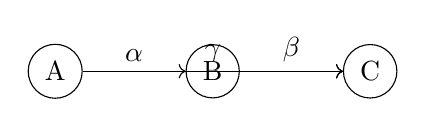
\begin{tikzpicture}
\node[draw,circle] (A) at (0,0) {A};
\node[draw,circle] (B) at (2,0) {B};
\node[draw,circle] (C) at (4,0) {C};
\draw[->] (A) -- node[midway,above] {$\alpha$} (B);
\draw[->] (B) -- node[midway,above] {$\beta$} (C);
\draw[->] (A) -- node[midway,above] {$\gamma$} (C);
\end{tikzpicture}
$$

\par\medskip
That is, $F_{\text{Hom}}(A, C) \circ F_{\text{Hom}}(B, A) = F_{\text{Hom}}(B, C)$.

\par\medskip
\item For every object $A$ in $\mathcal{C}$, the identity morphism on $A$ in $\mathcal{C}$ is mapped to the identity morphism on $F(A)$ in $\mathcal{D}$.

\par\medskip
\end{itemize}

\par\medskip
\textit{Universal constructions} are a powerful tool for building new mathematical objects from existing ones. They provide a way to find "the most general" object with certain properties, up to isomorphism. 

\par\medskip
For example, the product of two sets is a universal construction: given any two sets $A$ and $B$, there exists a unique set $A \times B$ together with projections $\pi_1: A \times B \rightarrow A$ and $\pi_2: A \times B \rightarrow B$ such that for any other set $C$ and functions $f: C \rightarrow A$ and $g: C \rightarrow B$, there exists a unique function $h: C \rightarrow A \times B$ satisfying $f = \pi_1 \circ h$ and $g = \pi_2 \circ h$.

\par\medskip
Universal constructions are essential for understanding many fundamental concepts in mathematics, including limits, colimits, and free objects.


\section{데이터베이스란 무엇인가?}
\label{sec:3-1}

요즘 산업 분야에서 여러 출처의 데이터를 통합하는 것은 주요 문제입니다. 2008\hspace{0pt}년 [BH08]의 연구에 따르면 데이터 통합이 IT(정보 기술) 예산의 40\%를 차지하며, 2007\hspace{0pt}년에는 데이터 통합 소프트웨어 시장이 25\hspace{0pt}억 달러였으며 연간 8\% 이상의 성장률을 보이고 있습니다. 다시 말해, 이는 중요한 문제이며, 그렇다면 무엇인가요?

\par\medskip
데이터베이스는 상호 연결된 테이블의 시스템입니다. 데이터는 저장되는 형태에 따라 정보가 됩니다. 즉, 숫자와 문자는 구성될 때까지 의미를 가지지 않습니다. 종종 상호 연결된 테이블 시스템으로 구성됩니다. 정돈된 상호 연결된 테이블 시스템을 데이터베이스라고 합니다. 다음은 예시입니다:

\par\medskip
직원
FName
WorksIn
Mngr
알란
루스
크리스
부서
DName
Secr
Sales
IT
(3.1)

\par\medskip
이 두 개의 테이블은 좌측 열에 있는 특별한 수평선으로 연결됩니다. 이를 ID 열이라고 합니다. 첫 번째 테이블의 ID 열을 '직원'이라고 하고, 두 번째 테이블의 ID 열을 '부서'라고 합니다. ID 열에 있는 항목—예: 1, 2, 3 또는 101, 102—은 행 레이블과 같습니다. 그들은 자신들이 속한 테이블의 전체 행을 나타냅니다. 따라서 각 행 레이블은 고유해야 하며 (테이블 내에서 같은 레이블을 가진 두 행이 있을 수 없습니다.) 그 행을 명확하게 지정할 수 있어야 합니다.

\par\medskip
각 테이블의 ID 열과 그 안에 있는 고유 식별자 집합은 위에서 언급한 상호 연결을 가능하게 합니다. 실제로 다양한 테이블의 다른 항목은 ID 열을 사용하여 특정 테이블의 행을 참조할 수 있습니다. 예를 들어, WorksIn 열의 각 항목은 각 직원에 대한 부서를 참조하며, Mngr(책임자) 열의 각 항목은 각 직원에 대한 직원을 참조하고, Secr(비서) 열의 각 항목은 각 부서에 대한 직원을 참조합니다. 이러한 모든 교차 참조 관리가 데이터베이스의 목적입니다.

\par\medskip
식 (3.1)를 다시 살펴보면, 두 테이블에서 모두 ID 열이 아닌 모든 열은 어떤 종류의 레이블을 참조하는 것입니다. 그중 WorksIn, Mngr, Secr\hspace{0pt}와 같은 것은 내부 참조이며, 자주 외래 키라고 불리며, 일부(외래) 테이블의 ID 열(키)에 있는 행(키)를 참조합니다. FName\hspace{0pt}과 DName\hspace{0pt}와 같이 다른 것들은 외부 참조이며, 의미가 더 광범위하게 알려진 문자열 또는 정수를 참조하는 것입니다. 내부 참조 레이블은 일관성이 유지되는 한 변경될 수 있습니다—1\hspace{0pt}을 모든 곳에서 1001\hspace{0pt}로 바꾸더라도 의미가 변하지 않기 때문입니다.— 반면에 외부 참조 레이블은 분명히 변경할 수 없습니다! 루스를 브루스로 모든 곳에서 변경하면 사람들이 데이터를 이해하는 방식이 달라집니다.

\par\medskip
특정 데이터베이스의 참조 구조—즉, 외래 키를 통해 테이블이 상호 연결되는 방식—은 그 안에 저장될 정보에 대해 알려줍니다. 식 (3.1)의 참조 구조를 다음과 같이 그래프로 시각화할 수 있습니다.

\par\medskip
직원
•
부서
•
WorksIn
Mngr
Secr
easySchema B
(3.2)

\par\medskip
FName
DName
string
◦

\par\medskip
이는 Remark 1.39\hspace{0pt}에서 언급된 사전 순서에 대한 Hasse 다이어그램과 유사한 것입니다. 어떻게 읽으면 좋을까요?

\par\medskip
식 (3.1)의 두 개의 테이블은 그래프 (3.2)에서 Employee\hspace{0pt}와 Department\hspace{0pt}라는 이름으로 표시된 두 개의 검정색 노드로 나타납니다. 다른 노드—검정색이 아닌 흰색으로 그려진 것—은 "알란", "알파", "Sales"와 같은 문자열과 같이 외부 참조 유형을 나타냅니다. 다이어그램의 화살표는 테이블의 ID 열이 아닌 항목을 나타내며, 참조 방향으로 가리킵니다: WorksIn\hspace{0pt}은 직원이 부서에 연결됩니다.

\par\medskip
문제 3.3 .
식 (3.1)에서 ID 열이 아닌 열의 수를 세십시오. 식 (3.2)에서 외래 키(화살표)의 수를 세십시오. 이 경우 동일한 수인가요? 이는 우연의 일치입니까?

\par\medskip
♦

\par\medskip
위와 같은 Hasse 스타일 다이어그램을 데이터베이스 스키마라고 합니다. 정보가 어떻게 구성되어 있는지, 데이터가 저장되는 형태를 나타냅니다. 데이터의 무결성을 보장하기 위해 스키마에 규칙, 때로는 '사업 규칙'이라고 불리는 규칙을 추가할 수 있습니다. 이러한 규칙이 위반되면 입력되는 데이터가 데이터베이스 설계자가 의도한 방식으로 일치하지 않는다는 것을 알 수 있습니다. 예를 들어, 설계자들은 다음과 같은 규칙을 적용하도록 할 수 있습니다.

\par\medskip
• 모든 부서의 비서는 그 부서에서 일해야 합니다.
• 모든 직원의 책임자는 해당 직원과 같은 부서에서 일해야 합니다.

\par\medskip
이렇게 하면 스키마가 'easySchema' (3.2) 에서 'mySchema'로 변경됩니다.

\par\medskip
직원
•
부서
•
WorksIn
Mngr
Secr
mySchema B
(3.4)

\par\medskip
FName
DName
string
◦

\par\medskip
즉, easySchema\hspace{0pt}에 제약 조건을 더하면 mySchema\hspace{0pt}가 됩니다.

\par\medskip
곧 데이터베이스 스키마는 카테고리 C\hspace{0pt}이며, 데이터 자체는 C → Set\hspace{0pt}의 '집합값' 함수로 주어지며, 데이터베이스는 C → D 함수를 통해 서로 매핑될 수 있습니다. 다시 말해, 데이터베이스 이론과 카테고리 이론 사이에는 상당한 겹침이 있습니다. 이것은 여러 논문에서 연구되었으며, Section 3.6\hspace{0pt}을 참조하십시오. 또한 FQL(함수형 쿼리 언어)이라는 이름의 작동하는 소프트웨어로 구현되었습니다. 위에 표시된 스키마에 대한 예제 FQL 코드입니다:

\par\medskip
schema mySchema = {
nodes
Employee, Department;
attributes
DName : Department -> string,
FName : Employee
-> string;
arrows
Mngr
: Employee
-> Employee,
WorksIn : Employee
-> Department,
Secr
: Department -> Employee;
equations
Department.Secr.WorksIn = Department,
Employee.Mngr.WorksIn
= Employee.WorksIn;
}

\par\medskip
데이터베이스 간의 통신

\par\medskip
우리는 데이터베이스가 어떤 것에 대한 정보를 저장하도록 설계되었다고 말했습니다. 하지만 다른 사람이나 기관은 같은 종류의 것을 다르게 볼 수 있습니다. 예를 들어, 한 은행이 유럽 표준에 따라 재무 기록을 저장하고 다른 은행이 일본 표준에 따라 저장한다면 두 은행이 하나로 합병되면 데이터베이스 스키마의 형태가 다르더라도 그들의 데이터를 공유할 수 있어야 합니다.

\par\medskip
데이터 마이그레이션: 카테고리 이론적 접근

\par\medskip
---

\par\medskip
일반적으로 이러한 문제는 매우 크고 복잡하며, 데이터베이스가 종종 수백 또는 수천 개의 연결된 테이블로 구성되어 있기 때문입니다. 또한, 회사들이 합병하려 할 때뿐만 아니라 더 자주 발생합니다. 특정 기업이 매일 데이터베이스 간에 데이터를 옮길 만큼 흔한 일입니다. 그 이유는 정보를 조직하는 다양한 방법이 다양한 목적에 적합하기 때문입니다. 우리가 여행할 때 옷을 캐리어에 넣고 집에서는 옷장을 사용하듯이, 어떤 것을 조직하는 가장 좋은 방법은 하나로 정해져 있지 않습니다.

\par\medskip
카테고리 이론은 이러한 다양한 조직 형태 간에 번역하는 수학적 접근 방식을 제공합니다. 즉, 데이터 마이그레이션이라는 자동화된 재조직 과정을 공식화하며, 하나의 스키마에 맞는 데이터를 다른 스키마로 이동시킵니다.

\par\medskip
다음은 간단한 예입니다. 상상해 보세요, 항공사가 두 개의 서로 다른 데이터베이스가 있고, 각각은 거의 같은 데이터를 저장하고 있습니다. 
$ ◦
$ ◦
가격
가격
가격
경제석
•
퍼스트 클래스
•
항공석
•
A B
 : B
위치
위치
위치
문자열
◦
문자열
◦
(3.5)

\par\medskip
스키마 A\hspace{0pt}는 스키마 B\hspace{0pt}보다 더 자세한 정보를 가지고 있습니다 — 항공석이 퍼스트 클래스 또는 경제석에 있을 수 있다는 점—하지만 그들은 대체로 동일합니다. 이러한 스키마들이 functors 로 연결될 수 있으며, A 에 맞는 데이터가 이 functors 를 통해 스키마 B 로 이동되고 반대로 이동될 수 있다는 것을 보여드리겠습니다.

\par\medskip
이 단락의 처음 부분에 나온 통계는 기업 규모에서 발생하는 이러한 문제가 여전히 어렵고 비싸다는 것을 보여줍니다. 원본 스키마에서 대상 스키마로 데이터를 이동하려고 하면, 이전된 데이터가 대상 스키마에 맞지 않거나 일부 제약 조건을 충족하지 못할 수 있습니다. 이는 사업 세계에서 놀랍게도 자주 발생합니다: 한 밤 동안 데이터를 옮기고 다음 아침에는 데이터가 손상되어 추가 사용에 적합하지 않은 것으로 발견되는 경우가 많습니다. 사실, 데이터베이스 마이그레이션 프로젝트의 절반 이상이 실패한다고 알려져 있습니다.

\par\medskip
이 장에서는 카테고리 이론적 방법을 사용하여 데이터를 마이그레이션하는 방법에 대해 논의합니다. 카테고리와 functors 를 사용하면 특정 데이터 마이그레이션이 실패하지 않음을 증명할 수 있습니다. 즉, 결과가 대상 스키마에 맞게 들어가 모든 제약 조건을 충족한다는 것을 보장할 수 있습니다.

\par\medskip
이 장의 내용은 카테고리 이론의 가장 중요한 부분을 다룹니다: 특히 카테고리, functors, 자연 변환, adjunctions, limits, 그리고 colimits\hspace{0pt}를 논의합니다. 실제로 위에서 언급된 많은 개념들이 다음과 같이 이미 논의되어 있습니다:
• 스키마 그림, 예를 들어 Eq. ( 3.4 )는 카테고리 C 를 나타냅니다.
• 인스턴스, 예를 들어 Eq. ( 3.1 )는 Set 라는 특정 카테고리로부터 functors 입니다.
• Eq. ( 3.5 )에서 암시된 매핑은 A 에서 경제석과 퍼스트 클래스 자리를 B 에서 항공석으로 가져가는 functors A → B 를 구성합니다.
• 스키마 간에 데이터를 이동하는 데이터 마이그레이션 개념은 adjunctions 로 공식화됩니다.

\par\medskip
3.2 절에서 카테고리의 정의와 다양한 유형의 예시들을 시작으로 설명합니다. 3.3 절에서는 데이터베이스, 특히 그들의 인스턴스와 그들 사이의 매핑을 functors 와 자연 변환을 통해 논의하여 다시 소개합니다. 3.4 절에서는 adjunctions\hspace{0pt}를 통해 데이터 마이그레이션을 논의하며, 이는 1.4 절에서 소개한 Galois 연결을 일반화합니다. 마지막으로 3.5 절에서는 limits\hspace{0pt}와 colimits\hspace{0pt}에 대한 보너스 섹션을 제공합니다.

\begin{deepresearch}{맞물리는 테이블 (Interlocking tables)}
카테고리 이론에서 "교차 테이블"은 다양한 카테고리 사이의 관계를 나타내는 도구입니다. 각 테이블 행과 열은 다른 카테고리를 나타내며, 교차하는 위치에는 두 카테고리 사이의 함수나 변환이 표시됩니다. 이러한 구조는 복잡한 시스템을 단순화하고 다양한 데이터 소스를 연결하는 데 유용합니다.
\\[4pt]{\footnotesize\color{ctgray} 출처: Wikipedia — Byford Dolphin}
\end{deepresearch}

\begin{deepresearch}{아이디 열 (ID column)}
데이터베이스에서 각 레코드를 고유하게 식별하기 위해 사용되는 열을 ID 열이라고 합니다.  ID 열은 일반적으로 정수형으로 구성되며, 다른 테이블과의 관계를 설정하는 데에도 중요한 역할을 합니다.
\\[4pt]{\footnotesize\color{ctgray} 출처: Wikipedia — SQLAlchemy}
\end{deepresearch}

\begin{deepresearch}{참조 (Cross-referencing)}
카테고리 이론에서 데이터를 통합하는 것은 중요한 문제입니다.  다른 출처에서 가져온 데이터를 연결하고 관계를 파악하기 위해서는 'cross-referencing'이라는 기술을 사용합니다.  이는 특정 개념이나 주제에 대한 추가 정보나 관련된 내용을 다른 부분에서 찾는 것을 의미하며, 이론적 이해를 넓히고 체계적인 시각을 제공하는 데 도움이 됩니다.
\\[4pt]{\footnotesize\color{ctgray} 출처: Wikipedia — Cross-reference}
\end{deepresearch}


\section{범주}
\label{sec:3-2}

한 범주 C\hspace{0pt}는 사물, 준동형, 항등원, 그리고 합성 규칙과 같은 네 가지 데이터로 구성되며 두 가지 성질을 만족합니다.

\par\medskip
\begin{definitionbox}[정의 3.6.]
범주 C\hspace{0pt}를 명시하려면:
(i) 하나는 Ob(C)라는 집합을 명시하며, 그 원소들을 사물이라고 합니다.
(ii) 모든 두 사물 c, d\hspace{0pt}에 대해, 하나는 C(c, d)라는 집합을 명시하며, 그 원소들을 c\hspace{0pt}에서 d\hspace{0pt}로 가는 준동형이라고 합니다.
(iii) 모든 사물 c ∈ Ob(C)에 대해, 하나는 id<sub>c</sub> ∈ C(c, c)인 준동형을 명시하며, 이를 c\hspace{0pt}의 항등 준동형이라고 합니다.
(iv) 모든 세 사물 c, d, e ∈ Ob(C)와 준동형 f ∈ C(c, d) 및 1 ∈ C(d, e)에 대해, 하나는 f \# 1 ∈ C(c, e)인 준동형을 명시하며, 이를 f\hspace{0pt}와 1\hspace{0pt}의 합성이라고 합니다.
때로는 c ∈ C, 대신 c ∈ Ob(C)를 쓰기도 합니다. 또한 f ∈ C(c, d)를 f : c → d\hspace{0pt}로 나타내는 것도 편리합니다. 여기서 c\hspace{0pt}는 f\hspace{0pt}의 정의역이고, d\hspace{0pt}는 f\hspace{0pt}의 공역입니다.
이러한 구성 요소들은 다음 두 가지 조건을 만족해야 합니다:
(a) 항등성: 어떤 준동형 f : c → d\hspace{0pt}에 대해, c 또는 d\hspace{0pt}에서의 항등 준동형과 합성하면 아무런 변화가 없습니다: id<sub>c</sub> \# f = f 및 f \# id<sub>d</sub> = f .
(b) 결합법칙: 세 준동형 f : c<sub>0</sub> → c<sub>1</sub>, 1 : c<sub>1</sub> → c<sub>2</sub>, 그리고 h : c<sub>2</sub> → c<sub>3</sub>에 대해, 다음이 같습니다: (f \# 1) \# h = f \# (1 \# h). 이 합성을 단순히 f \# 1 \# h\hspace{0pt}로 쓰기도 합니다.
1 “보너스”라고 말하는 것은 특정 장의 이해에 필수적이지 않지만, 한계와 공한계는 이 책과 카테고리 이론과의 상호 작용에서 어디에서나 나타날 것이며, 독자가 오랫동안 이 자료로부터 특히 이점을 얻게 될 것입니다.
2 여기서 집합은 세트처럼 많은 것들의 모임이라고 생각할 수 있지만, 공식적으로 세트가 되지 않을 수도 있습니다. 예를 들어 모든 세트의 집합은 스스로 세트가 된다면 러셀의 역설에 부딪힐 것입니다.
3 이 집합 C(c, d)는 종종 Hom<sub>C</sub>(c, d)로 나타내며, “c\hspace{0pt}에서 d\hspace{0pt}로 가는 준동형 집합”이라고 합니다. "hom"은 준동형을 뜻하며, "morphism"은 그 단축된 형태입니다.
다음 목표는 많은 카테고리의 예를 들어보는 것입니다. 우리가 처음으로 사용하는 예들은 자유로운 카테고리와 유한하게 제시된 카테고리이며, Remark 1.39\hspace{0pt}에서 언급된 Hasse 다이어그램 개념을 일반화합니다.
\end{definitionbox}


\begin{deepresearch}{물건 (Objects)}
범주 C\hspace{0pt}의 구성 요소 중 하나인 '객체'는 범주의 기본적인 단위입니다.  각 객체는 독립적인 개념을 나타내며, 다른 객체와 연결될 수 있습니다. 예를 들어, 집합, 함수, 또는 심지어 수학적 정리 자체가 객체로 여겨질 수 있습니다.  두 객체 사이의 관계나 변환은 '모르피즘'이라고 부르는데, 이는 객체들을 연결하는 링크 역할을 합니다.
\\[4pt]{\footnotesize\color{ctgray} 출처: Wikipedia — Mathematical object}
\end{deepresearch}

\begin{deepresearch}{모르피즘 (Morphisms)}
범사는 카테고리 이론에서 구조를 보존하는 함수와 같은 개념을 일반화합니다. 예를 들어, 대수적 구조 사이의 준동형, 집합에서 다른 집합으로의 함수, 위상 공간 사이의 연속 함수가 있습니다. 범사는 두 객체(출처 및 목표)를 연결하며, 이들은 카테고리의 구성 요소입니다.  두 개의 범사를 합성하는 것은 함수 합성과 유사하게 정의되며, 결과 또한 범사가 됩니다.
\\[4pt]{\footnotesize\color{ctgray} 출처: Wikipedia — Morphism}
\end{deepresearch}

\begin{deepresearch}{구성 규칙 (Composition rule)}
범주 $C$의 구성 규칙은 두 개체 $c$, $d$ 사이의 사상들 집합 $C(c, d)$를 정의하는 것입니다.  쉽게 말해, 어떤 두 개체를 연결하는 '길'을 나타내는 규칙입니다. 이 규칙은 두 개체 사이에 존재할 수 있는 모든 가능한 '연결 방법'을 정의하며, 각 연결 방법은 특정 사상으로 표현됩니다.
\\[4pt]{\footnotesize\color{ctgray} 출처: Wikipedia — Composition (visual arts)}
\end{deepresearch}


\subsection{자유 범주}
\label{sec:3-2-1}

그래프 G = (V, A, s, t)에서 자유 범주 Free(G)를 정의합니다. 그래프의 정점 V\hspace{0pt}는 자유 범주의 대상이며, c\hspace{0pt}와 d 사이의 경로는 c\hspace{0pt}와 d 사이의 사상입니다. 대상 c\hspace{0pt}에 대한 항등 사상은 c\hspace{0pt}에서 시작하여 c\hspace{0pt}에서 끝나는 삼각형 경로입니다. 합성은 경로 연결을 통해 주어집니다.

\par\medskip
예를 들어, 아래 그래프로 생성된 자유 범주 2\hspace{0pt}를 정의합니다.
(3.8)

\par\medskip
그래프는 두 개의 대상 v1\hspace{0pt}과 v2\hspace{0pt}와 세 가지 사상: idv1 : v1 → v1, f1 : v1 → v2, idv2 : v2 → v2\hspace{0pt}을 가지고 있습니다. 여기서 idv1\hspace{0pt}은 v1\hspace{0pt}에서 시작하여 v1\hspace{0pt}에서 끝나는 길이 0\hspace{0pt}인 경로입니다. f1\hspace{0pt}은 f1 하나만으로 구성된 길이 1\hspace{0pt}의 경로이며, idv2\hspace{0pt}는 v2\hspace{0pt}에서 시작하여 v2\hspace{0pt}에서 끝나는 길이 0\hspace{0pt}인 경로입니다. 우리의 기호처럼 idv1\hspace{0pt}은 대상 v1\hspace{0pt}에 대한 항등 사상이고, idv2\hspace{0pt}는 v2\hspace{0pt}에 대한 항등 사상입니다. 합성이 경로 연결을 통해 주어지므로, 예를 들어 idv1 \# f1 = f1, idv2 \# idv2 = idv2\hspace{0pt}와 같습니다.

\par\medskip
앞으로는 그래프와 해당하는 자유 범주 Free(G) 사이의 차이를 명확하게 이해할 수 있는 경우에만 구분을 생략합니다.

\par\medskip
\textbf{문제 3.9.}

\par\medskip
Free(G)가 진정한 범주가 되기 위해서는 우리가 지정한 이 데이터가 단위성과 결합성을 만족하는지 확인해야 합니다. 모든 그래프 G\hspace{0pt}에서 이것들이 충족되는지 확인하십시오.

\par\medskip
\textbf{문제 3.10.}

\par\medskip
다음 그래프에 대한 자유 범주:
(3.11)

\par\medskip
세 대상과 여섯 가지 사상을 가지고 있습니다. 세 개의 정점과 그래프에서의 여섯 가지 경로입니다. 각각의 여섯 가지 사상에 대해 여섯 가지 이름을 만들어 보세요. 열과 행이 위에서 선택한 여섯 가지 이름으로 표시된 여섯 개의 행렬을 작성하십시오.

\par\medskip
1. 합성이 있는 경우, 각 셀에 합성의 이름을 적으십시오.
2. 항등은 어디에 있나요?

\par\medskip
\textbf{문제 3.12.}

\par\medskip
위 패턴을 기반으로 몇 가지 정의를 만들어 보겠습니다.

\par\medskip
1. 범주 1\hspace{0pt}은 무엇입니까? 그 대상과 사상이 무엇인가요?
2. 범주 0\hspace{0pt}은 무엇입니까?
3. 임의의 n ∈ N\hspace{0pt}에 대한 n\hspace{0pt}에서의 사상 수 공식은 무엇입니까?

\par\medskip
\textbf{예시 3.13 (자연수는 자유 범주로서)} 다음 그래프를 고려하십시오.

\par\medskip
(3.14)

\par\medskip
그것은 하나의 정점과 하나의 화살만 가지고 있지만, 경로가 무한히 많습니다. 실제로, N ∈ N\hspace{0pt}에서 길이 n\hspace{0pt}인 유일한 경로가 있습니다. 즉, Path = {z, s, (s \# s), (s \# s \# s), ...}, 우리는 z\hspace{0pt}를 z\hspace{0pt}에서 시작하여 끝나는 길이 0\hspace{0pt}의 경로로 나타냅니다. 이것은 id z\hspace{0pt}를 나타내는 사상입니다. Path\hspace{0pt}와 자연수 N = {0, 1, 2, 3, ...} 사이에는 일대일 대응 관계가 있습니다.

\par\medskip
이는 하나의 대상을 가진 범주에 대한 예입니다. 하나의 대상을 가진 범주를 모노이드라고 합니다. 이 개념은 예시 2.6\hspace{0pt}에서 처음 언급했습니다. 그곳에서는 모노이드를 M, \textit{, e)로 정의했는데, } : M × M → M\hspace{0pt}이고 e ∈ M\hspace{0pt}이며, m \textit{ 1 = m = 1 } m 그리고 (m \textit{ n) } p = m \textit{ (n } p)입니다.

\par\medskip
두 개념은 표면적으로 다르게 보일 수 있지만 연결을 설명하는 것은 간단합니다. 하나의 대상 • 을 가진 범주 C\hspace{0pt}가 주어지면, M = C(•, •), e = id •, 그리고 \textit{ : C(•, •) × C(•, •) → C(•, •)를 } = \#로 정의하십시오. 모노이드의 결합성과 단위성 요구 사항은 범주 C\hspace{0pt}가 범주이기 때문입니다.

\par\medskip
\textbf{문제 3.15.}

\par\medskip
예시 3.13\hspace{0pt}에서 루프 그래프 (3.14)의 경로를 N ∈ N\hspace{0pt}의 수와 동일하게 식별했습니다. 경로를 연결할 수 있습니다. m, n ∈ N\hspace{0pt}이 주어진 경우, 해당 경로를 연결한 수는 무엇입니까?

\begin{deepresearch}{길 (Paths)}
범주 이론에서 경로는 두 점을 연결하는 연속적인 함수를 의미합니다.  특정 공간 내의 모든 점들을 연결할 수 있는 경로가 존재하면 그 공간은 경로 연결되어 있다고 합니다. 예를 들어, 그래프에서 정점 사이를 연결하는 화살표들의 순서인 경로는 시작 정점과 끝 정점을 가지며, $p: v \rightarrow w$ 와 같이 표현됩니다.
\\[4pt]{\footnotesize\color{ctgray} 출처: Wikipedia — Path (topology)}
\end{deepresearch}

\begin{deepresearch}{경로 구성 (Composition of Paths)}
그래프에서 경로는 화살의 순차적인 연결이며, 시작 정점과 끝 정점을 가집니다.  $p : v \rightarrow w$ 와 같이 $p$가 $v$ 에서 $w$ 로 가는 경로라고 표현하며, $v$ 에서 출발하여 $v$ 에 도착하는 단순한 경로는 $id_v$ 또는 간단히 $id$ 로 나타냅니다.  각 정점은 시작과 끝이 같은 경로를 가지며, 이는 그 정점에서 멈추지 않는 경로입니다.
\\[4pt]{\footnotesize\color{ctgray} 출처: Wikipedia — Six Paths}
\end{deepresearch}


\subsection{범주를 나타내는 유한 표현}
\label{sec:3-2-2}

어떤 그래프 G\hspace{0pt}에 대해, 항상 G\hspace{0pt}에서 자유 범주가 존재합니다. 하지만 우리는 여기서 끝낼 필요가 없습니다: 우리는 그래프의 경로 사이에 방정식을 추가할 수 있으며, 여전히 범주를 얻을 수 있습니다. 우리는 두 경로 p\hspace{0pt}와 q\hspace{0pt}를 같다고 할 수 있는 것은 병렬인 경우 뿐입니다. 즉, 같은 출발 정점과 같은 도착 정점을 가진 경우입니다.

\par\medskip
경로 방정식이 있는 유한 그래프를 범주의 유한 표현이라고 하고, 결과적으로 얻는 범주를 유한으로 제시된 범주라고 합니다. 다음은 두 가지 예입니다:

\par\medskip
f
f
A •
B •
A •
B •
h
h
Free\_square B
Comm\_square B
•
C
•
D
•
C
•
D
i
i
f \# h  1 \# i
no equations
위의 두 가지는 모두 범주의 표현입니다: 왼쪽 그림에는 방정식이 없기 때문에, 3.2.1\hspace{0pt}절에서 논의한 것처럼 자유 범주를 나타냅니다. 자유 사각형 범주에는 열 개의 형이동이 있습니다. 모든 경로가 고유한 형이동이기 때문입니다.

\par\medskip
\textbf{예제 3.16.}
1. 위의 자유 사각형 범주에서 열 개의 경로를 적으시오.
2. 병렬인 두 가지 다른 경로를 명명하시오.
3. 병렬이 아닌 두 가지 다른 경로를 명명하시오.

\par\medskip
♦

\par\medskip
반면에, 오른쪽 그림으로 제시된 범주에는 단지 아홉 개의 형이동만 있습니다. 왜냐하면 f \# h\hspace{0pt}와 1 \# i\hspace{0pt}가 같다고 설정되었기 때문입니다. 이 범주는 "commutative square"라고 불립니다. 그 형이동은
{ A , B , C , D , f , 1 , h , i , f \# h }
로 주어집니다. 어떤 사람이 “누락된 것은 1 \# i 입니다.”라고 말할 수 있지만, 그것은 정확하지 않습니다: 1 \# i\hspace{0pt}는 존재합니다. 왜냐하면 f \# h\hspace{0pt}와 같기 때문입니다. 일반적으로 A\hspace{0pt}는 id A\hspace{0pt}를 나타내고, 등등입니다.

\par\medskip
\textbf{예제 3.17.} 다음 그림으로 제시된 범주에서 모든 형이동을 적으시오:
f
A •
B •
j
h
•
C
•
D
i
f \# h  j  1 \# i
♦

\par\medskip
\textbf{예제 3.18.} 두 형이동 사이에 방정식을 강요하는 것은 종종 추가적인 방정식을 함의한다는 점도 알아야 합니다. 이러한 현상이 발생하는 두 가지 더 많은 예를 보여줍니다:

\par\medskip
s
s
C B
•
z
D B
•
z
s \# s  z
s \# s \# s \# s  s \# s
위의 C\hspace{0pt}에서 방정식 s \# s  z\hspace{0pt}가 있습니다. 하지만 이것은 s \# s \# s  z \# s  s!를 함의합니다. 그리고 마찬가지로 s \# s \# s \# s  z \# z  z 를 가집니다. 실제로 C\hspace{0pt}에서의 형이동 집합은 { z , s }이며, 합성은 s \# s  z \# z  z 와 z \# s  s \# z  s 로 설명됩니다. 군 이론에서는 Z / 2 Z 라는 군에 대해 말할 수 있습니다.

\par\medskip
\textbf{예제 3.19.}
예시 3.18\hspace{0pt}에서 D 범주에서 모든 형이동을 적으시오.

\par\medskip
♦

\par\medskip
\textbf{참고 3.20.} 이제 3.1\hspace{0pt}절의 스키마, 예를 들어 ( 3.2 )와 ( 3.4 )가 유한 범주의 표현임을 알 수 있습니다. 이 아이디어는 3.3\hspace{0pt}절에서 다시 살펴보겠습니다.

\begin{center}
\includegraphics[width=0.7\textwidth]{images/p96_d0.png}
\end{center}

\begin{center}
\includegraphics[width=0.7\textwidth]{images/p97_d0.png}
\end{center}

\begin{deepresearch}{유한 표현 (Finite presentation)}
유한 그래프에 경로 방정식을 추가하면 특정 카테고리를 나타내는 유한 표현이라고 합니다.  각 경로가 같은 출발점과 도착점을 가진 경우만 두 경로를 동등하게 만들 수 있습니다. 이러한 유한 표현은 그래프에서 생성된 자유 카테고리에 경로 방정식을 적용하여 얻어집니다.
\\[4pt]{\footnotesize\color{ctgray} 출처: Wikipedia — Presentation of a group}
\end{deepresearch}

\begin{deepresearch}{무한히 제시된 범주 (Fintely-presented category)}
유한 그래프에 경로 간 방정식을 추가하면 얻는 카테고리를 유한 표현이라고 합니다.  그래프의 각 정점은 카테고리의 대상이며, 그래프의 변은 카테고리의 화살표를 나타냅니다. 두 경로가 같은 출발점과 도착점을 가진 경우(즉, 병렬인 경우)만 같다고 할 수 있습니다. 이러한 유한 표현으로 정의된 카테고리를 유한하게 제시된 카테고리라고 합니다.
\\[4pt]{\footnotesize\color{ctgray} 출처: Wikipedia — 2024 European Parliament election in Italy}
\end{deepresearch}

\begin{deepresearch}{병렬 경로 (Parallel paths)}
그래프 $G$ 에 대해 자유 카테고리 $\mathcal{C}$를 만들 수 있습니다. 하지만 그래프의 경로 사이에 방정식을 추가하여 더욱 풍부한 카테고리를 만들 수도 있습니다. 두 경로 $p$ 와 $q$ 가 같은 출발 정점과 같은 도착 정점을 가지면, 즉 병렬 경로라면 서로 같다고 할 수 있습니다. 이러한 방정식을 사용하여 생성된 유한 그래프를 카테고리의 유한 표현이라고 합니다.
\\[4pt]{\footnotesize\color{ctgray} 출처: Wikipedia — Critical path method}
\end{deepresearch}


\subsection{순서쌍과 자유 범주: 스펙트럼의 양 끝}
\label{sec:3-2-3}

이제 우리가 제\hspace{0pt}1\hspace{0pt}장에서 순서쌍을 그리고 위에서 범주를 그래프로 표현한 것을 알고 있다면, 이 두 사용 사이의 관계에 대해 알고 싶어할 수 있습니다. 지금 설명하고자 하는 주요 아이디어는 “순서쌍은 모든 두 개의 평행 화살이 같은 범주이다”라는 것입니다. 따라서 어떤 순서쌍을 범주로 간주할 수 있으며, 어떤 범주를 어떻게든 "압축"하여 순서쌍으로 만들 수 있습니다. 이러한 아이디어에 대해 논해 보겠습니다.

\par\medskip
순서쌍을 범주로서

\par\medskip
가정하자 ( P , ≤) 는 순서쌍입니다. 다음과 같이 P 를 범주로 정의합니다. P 의 대상은 P 의 요소와 정확히 일치합니다; 즉, Ob(P) = P 입니다. 준동형에 관해서는 p ≤ q 이면 P 에 p → q 가 정확히 하나의 준동형이 있고, p ≰ q 이면 p → q 는 없는 준동형입니다. ≤ 가 반사적임은 모든 대상이 항등원을 가지도록 보장하며, ≤ 가 전이적임은 준동형이 합성될 수 있음을 보장합니다. P 를 순서쌍 (P , ≤) 에 해당하는 범주라고 부릅니다.

\par\medskip
실제로 순서쌍의 하세 다이어그램은 모든 정점 p 와 q 에 대해 p → q 로 가는 모든 경로가 같다고 선언되는 범주의 표현으로 생각할 수 있습니다. 예를 들어, (1.5) 에서 우리는 왼쪽에 있는 그래프와 같은 하세 다이어그램을 보았습니다:

\par\medskip
•
•
•
f
f
d
e
d
e
•
•
•
•
•
•
•
•
•
a
b
c
a
b
c
•
•
•
a \# d  b \# e  c \# f

\par\medskip
(1.5) 에서의 하세 다이어그램 (왼쪽)은 (가운데) 방정식 없이 자유 범주의 표현과 가장 유사해 보일 수 있지만, 그렇지 않습니다.

\par\medskip
자유 범주에는 아래 대상에서 위 대상으로 가는 경로가 세 개 있습니다. 반면 순서쌍은 두 주어진 대상 사이에 최대 하나의 준동형을 가진 범주입니다. 오히려 아래와 같이, 아래에서 위로 가는 경로들이 같도록 만든 다이어그램이 왼쪽 순서쌍에 대한 올바른 표현입니다.

\par\medskip
\textbf{문제 3.21.}

\par\medskip
아래 그래프에 어떤 방정식을 추가해야 해당 순서쌍을 나타낼 수 있습니까?

\par\medskip
f
f
•
•
•
•
f
G 1 
•
•
f
h
♦
G 2 
G 3 
G 4 
h
•
•
•
•
•
i

\par\medskip
범주의 순서쌍 반영

\par\medskip
어떤 범주 C 가 주어지면, 임의의 두 평행 준동형 사이의 차이를 없애는 것으로부터 (C , ≤) 순서쌍을 얻을 수 있습니다. 즉, C B Ob(C) 를 사용하고 c 1 ≤ c 2 iff C(c 1 , c 2) , œ 로 합니다. 만약 C 에서 c 1 → c 2 가 하나, 두 개, 다섯 개 또는 무한히 많은 준동형이 있다면, 순서쌍 반영은 차이를 보지 않습니다. 그러나 어떤 준동형과 아무런 준동형이 없는 것 사이의 차이는 알 수 있습니다.

\par\medskip
\textbf{문제 3.22.}

\par\medskip
예시 3.13 에서 나오는 N 범주의 순서쌍 반영은 무엇입니까?
♦

\par\medskip
우리는 이전에 순서쌍 사이의 대응 함수만 논했습니다. 하지만 곧 일반적인 대응 함수를 논의할 것입니다. 다음은 이해하기 어려운 명제이지만, 사실입니다; 카테고리 이론 전문가에게 물으면 설명해 줄 수 있습니다:

\par\medskip
순서쌍을 범주로 간주하는 것은 범주를 순서쌍 반영으로 변환하는 것에 대응합니다.

\par\medskip
\textbf{참고 3.23 (스펙트럼의 양 끝)}

\par\medskip
이 부분의 주요 내용은 순서쌍과 자유 범주가 모두 경로 방정식 없는 그래프로 특징 지어지지만 스펙트럼의 반대쪽을 나타내는 것입니다. 두 경우 모두 그래프의 정점이 범주의 대상이고 경로가 준동형이 됩니다. 하지만 자유 범주에서 경로가 없으므로 각 경로가 다른 준동형이 됩니다. 순서쌍의 경우 모든 평행 경로가 같은 준동형이 됩니다. 모든 카테고리 표현, 즉 일부 방정식을 가진 그래프는 자유 범주(모든 방정식 없음)와 그 순서쌍 반영(모든 가능한 방정식) 사이에 어디에 있습니까?

\begin{center}
\includegraphics[width=0.7\textwidth]{images/p97_d0.png}
\end{center}

\begin{deepresearch}{선주문 (Preorder)}
카테고리 이론에서 preorder\hspace{0pt}는 반사적이고 전이적인 이진 관계입니다.  즉, 모든 객체가 자신과 관련되며, $x$와 $y$가 $z$와 관련되어 있고 $y$와 $z$가 관련되어 있다면 $x$와 $z$도 관련된다는 의미입니다. 하지만 preorder\hspace{0pt}는 반대칭적이지 않아서, 예를 들어 2\hspace{0pt}와 4\hspace{0pt}는 각각 다른 객체이지만 서로를 포함한다는 관계에서 같은 preorder\hspace{0pt}에 속합니다.
\\[4pt]{\footnotesize\color{ctgray} 출처: Wikipedia — Preorder}
\end{deepresearch}

\begin{deepresearch}{카테고리 (Category)}
범주 이론에서 범주는 '객체'와 ' 화살표'로 연결된 집합입니다.  화살표들은 결합적으로 합성될 수 있고 각 객체마다 항등 화살표가 존재합니다. 예를 들어, 집합의 범주에서는 객체가 집합이고 화살표가 함수입니다.  즉, 범주는 다양한 수학적 개념들을 일반화하는 도구로 사용됩니다.
\\[4pt]{\footnotesize\color{ctgray} 출처: Wikipedia — Category (mathematics)}
\end{deepresearch}

\begin{deepresearch}{해스 다이어그램 (Hasse diagram)}
Hasse 다이어그램은 부분 순서 집합을 시각적으로 나타내는 도구입니다. 각 원소를 점으로 표현하고, 하나의 원소가 다른 원소를 덮는 관계($x \leq y$이고 $z$가 존재하지 않는 경우)일 때 그 두 점 사이에 선을 그어 연결합니다. 이 다이어그램은 부분 순서 집합의 구조를 간결하게 보여주며, 특히 최소 원소와 최대 원소를 쉽게 파악할 수 있습니다.
\\[4pt]{\footnotesize\color{ctgray} 출처: Wikipedia — Hasse diagram}
\end{deepresearch}


\subsection{수학에서 중요한 카테고리}
\label{sec:3-2-4}

카테고리 표현에 대해 이야기해 왔지만, 일부 카테고리는 표현을 통해 이해하기보다는 직접적으로 이해하는 것이 더 좋습니다. 
\begin{definitionbox}[정의 3.6]
에서 정의된 카테고리의 개념을 기억하십시오. 수학에서 가장 중요한 카테고리는 집합의 카테고리입니다.
\end{definitionbox}

\par\medskip
\begin{definitionbox}[정의 3.24.]
집합의 카테고리, Set 로 표기되며 다음과 같이 정의됩니다.
(i) Ob (Set) 는 모든 집합의 모임입니다.
(ii) S 와 T 가 집합일 경우, Set(S, T) = {f : S → T | f\hspace{0pt}는 함수} 입니다.
(iii) 각 집합 S 에 대해, 항등 사상은 id<sub>S</sub> : S → S 로 주어지며, id<sub>S</sub>(s) = s  모든 s ∈ S 에 대해서입니다.
(iv) f : S → T 와 1 : T → U 가 주어진 경우, 그들의 합성은 S → U 로 주어지는 함수 f \# 1 이며, (f \# 1)(s) = 1(f(s)) 입니다.
\end{definitionbox}

\par\medskip
이러한 정의는 단위성과 결합성 조건을 만족하므로 Set 은 실제로 카테고리입니다.
밀접하게 관련된 것은 FinSet 카테고리입니다. 이 카테고리는 대상이 유한 집합이며, 그 사상이 그들 사이의 함수인 카테고리입니다.

\par\medskip
예제 3.25.
2 = {1, 2} 와 3 = {1, 2, 3} 라고 하자. 이들은 
\begin{definitionbox}[정의 3.24]
에서 논의된 Set 카테고리의 대상입니다. Set(2, 3) 의 모든 요소를 적으세요; 아홉 개가 있어야 합니다.
\end{definitionbox}

\par\medskip
♦
주석 3.26. V-카테고리 (
\begin{definitionbox}[정의 2.46]
) 와 카테고리가 무엇과 관련이 있는지 궁금해했을 수 있습니다. 두 정의는 거의 비슷하게 보이지 않아도 될까요? '부가 구조를 가진 카테고리'라는 용어에도 불구하고, V-카테고리는 추가 구조를 가진 카테고리가 아닙니다. Bool-카테고리와 같은 일부 유형의 V-카테고리(즉, 순서)는 자연스럽게 카테고리로 볼 수 있지만, Cost-카테고리와 같은 다른 유형은 그렇지 않습니다.
\end{definitionbox}

\par\medskip
Set 의 중요성의 이유는, 부가 카테고리 (
\begin{definitionbox}[정의 2.46]
) 의 정의를 일반화하면, 정의 3.6 에서의 카테고리가 바로 Set-카테고리라는 것을 발견하기 때문입니다. 따라서 카테고리는 V 가 매우 특별한 선택인 V -카테고리입니다. 이는 4.4.4 절에서 다시 살펴보겠습니다. 지금은, Cost 카테고리에 대한 깊이 있는 이해(예: 그것은 Quantale\hspace{0pt}임을 알고 있다)가 Lawvere 거리 공간에 대한 통찰력을 제공하는 것처럼, Set 에 대한 연구는 카테고리에 대한 통찰력을 제공한다는 점만 간단히 언급하겠습니다.
\end{definitionbox}

\par\medskip
수학자들이 신경 쓰는 다른 많은 카테고리가 있습니다:
• Top : 위상 공간의 카테고리 (직교)
• Grph : 그래프의 카테고리 (연결)
• Meas : 측도 공간의 카테고리 (양)
• Mon : 단위들의 카테고리 (작용)
• Grp : 군의 카테고리 (역가능한 작용, 대칭성)
• Cat : 카테고리의 카테고리 (맥락에서의 작용, 구조)

\par\medskip
하지만 실제로는 수학자들이 생각하는 카테고리의 다양성을 제대로 보여주지 않습니다. 그들은 당시 목적에 맞는 카테고리를 사용합니다. 예를 들어 '차원이 4 이하인 연결된 리만 매니폴드의 카테고리' 와 같습니다.

\par\medskip
다음은 또 다른 예제 출처입니다: 이미 가지고 있는 어떤 카테고리든 모든 사상을 반전하면 다시 한 번 카테고리가 됩니다.

\par\medskip
예시 3.27. C\hspace{0pt}가 카테고리라고 하자.
그의 역, C op 로 표기되며 다음과 같습니다.
동일한 대상이 있습니다, Ob(C op) = Ob(C) , 그리고 어떤 두 대상 c, d ∈ Ob(C) 에 대해서, 하나는 C op (c, d) = C(d, c) 입니다. 항등 사상과 합성은 C 에서와 같습니다.

\begin{deepresearch}{비카테고리 (V-categories)}
세트의 개념을 일반화하여 만들어진 V-범주는 특정한 집합들의 관계를 나타내는 데 사용됩니다.  V-범주의 객체들은 집합이며, 화살표는 집합 사이의 함수를 나타냅니다. 이러한 범주는 집합론과 관련된 다양한 개념들을 이해하는데 유용하게 활용될 수 있습니다.
\\[4pt]{\footnotesize\color{ctgray} 출처: Wikipedia — Category (mathematics)}
\end{deepresearch}

\begin{deepresearch}{카테고리 설정 (Set-categories)}
집합 이론에서 가장 중요한 카테고리인 Set\hspace{0pt}은 집합들을 객체로 하고, 두 집합 사이의 함수를 사상으로 가지는 카테고리입니다.  즉, Set 에서는 모든 집합이 객체이며, 각 집합 사이에 존재하는 함수가 사상을 이룹니다. 이러한 사상들은 함수의 합성과 같은 연산을 통해 조합될 수 있습니다.
\\[4pt]{\footnotesize\color{ctgray} 출처: Wikipedia — Category of sets}
\end{deepresearch}

\begin{deepresearch}{핀셋 (FinSet)}
$FinSet$는 유한 집합들을 대상으로 하고, 이들 집합 사이의 함수들을 사상으로 하는 카테고리입니다. 즉, $FinSet$에서 각 대상은 유한 개의 원소를 가진 집합이며, 두 집합 사이의 함수가 그 집합들 사이의 사상이 됩니다.  이는 집합론과 관련된 다양한 개념들을 이해하는 데 유용하게 사용될 수 있습니다.
\\[4pt]{\footnotesize\color{ctgray} 출처: Wikipedia — FinSet}
\end{deepresearch}


\subsection{범주 내의 동형}
\label{sec:3-2-5}

이전 섹션들은 자유 범주, 제시된 범주 및 수학에서 중요한 범주와 같은 범주의 예에 대해 다루었습니다. 이 섹션에서는 범주 이론에서 중요한 개념인 동형 개념에 대해 간략하게 논의합니다.

\par\medskip
범주에서 두 개체가 서로 교환 가능하다는 아이디어가 자주 있습니다. 예를 들어, Set 범주에서 집합 { ■ , □ }을 집합 { 0 , 1 }으로 바꾸더라도 모든 것이 이름만 다르면 동일합니다. 마찬가지로, a, b 와 같은 원소를 가진 사전 순서가 a ≤ b 및 b ≤ a 이고 즉 a ≡ b 라면, a\hspace{0pt}와 b\hspace{0pt}는 본질적으로 같습니다. 어떻게 그런가요? 다른 개체 c 에 대해 c ≤ a iff c ≤ b , 그리고 c ≥ a iff c ≥ b 와 같이 동일하게 작용하기 때문입니다. 동형의 개념은 이러한 교환 가능성의 개념을 공식화합니다.

\par\medskip
\begin{definitionbox}[정의 3.28.]
동형은 f : A → B 라는 사상으로, f \# 1  id A 그리고 1 \# f  id B 를 만족하는 사상 1 : B → A 가 존재하는 것입니다. 이 경우 f 와 1 을 역사상이라고 부르며, 일반적으로 1  f − 1 또는 f  1 − 1 라고 쓰기도 합니다. 또한 A 와 B 를 동형 개체라고 말합니다.
\end{definitionbox}

\par\medskip
예제 3.29. 집합 A = { a , b , c } 와 집합 3 = { 1 , 2 , 3 } 는 동형입니다; 즉, f ( a )  2, f ( b )  1, f ( c )  3 로 주어진 사상 f : A → 3 가 존재합니다. Set 범주에서의 동형은 전단사 함수입니다.

\par\medskip
Recall that the cardinality of a finite set is the number of elements in it. This can be understood in terms of isomorphisms in FinSet . Namely, for any finite set A ∈ FinSet , its cardinality is the number n ∈ N such that there exists an isomorphism A  n . Georg Cantor defined the cardinality of any set X to be its isomorphism class, meaning the equivalence class consisting of all sets that are isomorphic to X .

\par\medskip
\begin{exercisebox}[연습문제 3.30.]
1. 예제 3.29\hspace{0pt}에서 주어진 함수 f 의 역함수 f − 1 : 3 → A 는 무엇입니까?
2. A → 3 로의 동형은 몇 개 있습니까?
\end{exercisebox}

\par\medskip
♦

\par\medskip
\begin{exercisebox}[연습문제 3.31.]
어떤 주어진 범주 C 에서, 임의의 개체 c ∈ C 에 대해 항등 사상 id c 가 동형임을 보여주세요.
♦
\end{exercisebox}

\par\medskip
\begin{exercisebox}[연습문제 3.32.]
예시 3.13\hspace{0pt}과 3.18 을 되돌아보세요. 모든 사상이 동형인 모노이드는 군으로 알려져 있습니다.
1. 예시 3.13\hspace{0pt}에서 제시된 모노이드는 군입니까?
\end{exercisebox}


\begin{deepresearch}{동형사상 (Isomorphism)}
이형성은 두 구조가 같은 형태를 가지고 있으면서 서로 변환될 수 있는 관계입니다.  $A \cong B$ 와 같이 표현되며, 이는 A\hspace{0pt}와 B\hspace{0pt}가 구조적으로 동일하다는 의미입니다. 즉, 추가적인 정보나 이름을 제외하고 두 구조는 구분할 수 없으며, 이형성에 대한 관점에서 동일하다고 할 수 있습니다.
\\[4pt]{\footnotesize\color{ctgray} 출처: Wikipedia — Isomorphism}
\end{deepresearch}

\begin{deepresearch}{모르피즘 (Morphisms)}
범주 이론에서 모르피즘은 집합 사이의 함수나 위상 공간 사이의 연속 함수와 같은 구조를 보존하는 지도를 일반화한 개념입니다. 두 객체를 연결하는 것처럼 생각하면 되는데,  이러한 연결은 함수 조합과 유사하게 구성될 수 있습니다. 즉, 모르피즘은 두 객체 간의 관계를 나타내는 도구이며, 이들을 조합하여 더 복잡한 관계를 표현할 수 있습니다.
\\[4pt]{\footnotesize\color{ctgray} 출처: Wikipedia — Morphism}
\end{deepresearch}

\begin{deepresearch}{카디널리티 (Cardinality)}
카테고리 이론에서 두 객체가 서로 대체 가능하다는 아이디어가 자주 등장합니다. 집합의 경우, 두 집합이 같은 크기를 가지면서 각 원소를 하나씩 매칭할 수 있다면, 그 집합은 \textbf{등원(isomorphic)} 입니다.  이는 집합의 \textbf{ Cardinality} 라는 개념과 직접적으로 관련되어 있습니다. 즉, 두 집합이 동일한\hspace{0pt}Cardinality\hspace{0pt}를 가질 때, 그들은 등원 관계에 있고 카테고리 이론에서도 유사하게 정의됩니다.
\\[4pt]{\footnotesize\color{ctgray} 출처: Wikipedia — Cardinality}
\end{deepresearch}


\end{document}